% Options for packages loaded elsewhere
\PassOptionsToPackage{unicode}{hyperref}
\PassOptionsToPackage{hyphens}{url}
\PassOptionsToPackage{dvipsnames,svgnames,x11names}{xcolor}
%
\documentclass[
  letterpaper,
  DIV=11,
  numbers=noendperiod]{scrreprt}

\usepackage{amsmath,amssymb}
\usepackage{lmodern}
\usepackage{iftex}
\ifPDFTeX
  \usepackage[T1]{fontenc}
  \usepackage[utf8]{inputenc}
  \usepackage{textcomp} % provide euro and other symbols
\else % if luatex or xetex
  \usepackage{unicode-math}
  \defaultfontfeatures{Scale=MatchLowercase}
  \defaultfontfeatures[\rmfamily]{Ligatures=TeX,Scale=1}
\fi
% Use upquote if available, for straight quotes in verbatim environments
\IfFileExists{upquote.sty}{\usepackage{upquote}}{}
\IfFileExists{microtype.sty}{% use microtype if available
  \usepackage[]{microtype}
  \UseMicrotypeSet[protrusion]{basicmath} % disable protrusion for tt fonts
}{}
\makeatletter
\@ifundefined{KOMAClassName}{% if non-KOMA class
  \IfFileExists{parskip.sty}{%
    \usepackage{parskip}
  }{% else
    \setlength{\parindent}{0pt}
    \setlength{\parskip}{6pt plus 2pt minus 1pt}}
}{% if KOMA class
  \KOMAoptions{parskip=half}}
\makeatother
\usepackage{xcolor}
\setlength{\emergencystretch}{3em} % prevent overfull lines
\setcounter{secnumdepth}{5}
% Make \paragraph and \subparagraph free-standing
\ifx\paragraph\undefined\else
  \let\oldparagraph\paragraph
  \renewcommand{\paragraph}[1]{\oldparagraph{#1}\mbox{}}
\fi
\ifx\subparagraph\undefined\else
  \let\oldsubparagraph\subparagraph
  \renewcommand{\subparagraph}[1]{\oldsubparagraph{#1}\mbox{}}
\fi


\providecommand{\tightlist}{%
  \setlength{\itemsep}{0pt}\setlength{\parskip}{0pt}}\usepackage{longtable,booktabs,array}
\usepackage{calc} % for calculating minipage widths
% Correct order of tables after \paragraph or \subparagraph
\usepackage{etoolbox}
\makeatletter
\patchcmd\longtable{\par}{\if@noskipsec\mbox{}\fi\par}{}{}
\makeatother
% Allow footnotes in longtable head/foot
\IfFileExists{footnotehyper.sty}{\usepackage{footnotehyper}}{\usepackage{footnote}}
\makesavenoteenv{longtable}
\usepackage{graphicx}
\makeatletter
\def\maxwidth{\ifdim\Gin@nat@width>\linewidth\linewidth\else\Gin@nat@width\fi}
\def\maxheight{\ifdim\Gin@nat@height>\textheight\textheight\else\Gin@nat@height\fi}
\makeatother
% Scale images if necessary, so that they will not overflow the page
% margins by default, and it is still possible to overwrite the defaults
% using explicit options in \includegraphics[width, height, ...]{}
\setkeys{Gin}{width=\maxwidth,height=\maxheight,keepaspectratio}
% Set default figure placement to htbp
\makeatletter
\def\fps@figure{htbp}
\makeatother
\newlength{\cslhangindent}
\setlength{\cslhangindent}{1.5em}
\newlength{\csllabelwidth}
\setlength{\csllabelwidth}{3em}
\newlength{\cslentryspacingunit} % times entry-spacing
\setlength{\cslentryspacingunit}{\parskip}
\newenvironment{CSLReferences}[2] % #1 hanging-ident, #2 entry spacing
 {% don't indent paragraphs
  \setlength{\parindent}{0pt}
  % turn on hanging indent if param 1 is 1
  \ifodd #1
  \let\oldpar\par
  \def\par{\hangindent=\cslhangindent\oldpar}
  \fi
  % set entry spacing
  \setlength{\parskip}{#2\cslentryspacingunit}
 }%
 {}
\usepackage{calc}
\newcommand{\CSLBlock}[1]{#1\hfill\break}
\newcommand{\CSLLeftMargin}[1]{\parbox[t]{\csllabelwidth}{#1}}
\newcommand{\CSLRightInline}[1]{\parbox[t]{\linewidth - \csllabelwidth}{#1}\break}
\newcommand{\CSLIndent}[1]{\hspace{\cslhangindent}#1}

\KOMAoption{captions}{tableheading}
\makeatletter
\makeatother
\makeatletter
\@ifpackageloaded{bookmark}{}{\usepackage{bookmark}}
\makeatother
\makeatletter
\@ifpackageloaded{caption}{}{\usepackage{caption}}
\AtBeginDocument{%
\ifdefined\contentsname
  \renewcommand*\contentsname{Table of contents}
\else
  \newcommand\contentsname{Table of contents}
\fi
\ifdefined\listfigurename
  \renewcommand*\listfigurename{List of Figures}
\else
  \newcommand\listfigurename{List of Figures}
\fi
\ifdefined\listtablename
  \renewcommand*\listtablename{List of Tables}
\else
  \newcommand\listtablename{List of Tables}
\fi
\ifdefined\figurename
  \renewcommand*\figurename{Figure}
\else
  \newcommand\figurename{Figure}
\fi
\ifdefined\tablename
  \renewcommand*\tablename{Table}
\else
  \newcommand\tablename{Table}
\fi
}
\@ifpackageloaded{float}{}{\usepackage{float}}
\floatstyle{ruled}
\@ifundefined{c@chapter}{\newfloat{codelisting}{h}{lop}}{\newfloat{codelisting}{h}{lop}[chapter]}
\floatname{codelisting}{Listing}
\newcommand*\listoflistings{\listof{codelisting}{List of Listings}}
\makeatother
\makeatletter
\@ifpackageloaded{caption}{}{\usepackage{caption}}
\@ifpackageloaded{subcaption}{}{\usepackage{subcaption}}
\makeatother
\makeatletter
\@ifpackageloaded{tcolorbox}{}{\usepackage[many]{tcolorbox}}
\makeatother
\makeatletter
\@ifundefined{shadecolor}{\definecolor{shadecolor}{rgb}{.97, .97, .97}}
\makeatother
\makeatletter
\makeatother
\ifLuaTeX
  \usepackage{selnolig}  % disable illegal ligatures
\fi
\IfFileExists{bookmark.sty}{\usepackage{bookmark}}{\usepackage{hyperref}}
\IfFileExists{xurl.sty}{\usepackage{xurl}}{} % add URL line breaks if available
\urlstyle{same} % disable monospaced font for URLs
\hypersetup{
  pdftitle={GIS for Urban Planning: QGIS methods},
  pdfauthor={Dr.~Kam Tin Seong},
  colorlinks=true,
  linkcolor={blue},
  filecolor={Maroon},
  citecolor={Blue},
  urlcolor={Blue},
  pdfcreator={LaTeX via pandoc}}

\title{GIS for Urban Planning: QGIS methods}
\author{Dr.~Kam Tin Seong}
\date{09/11/2022}

\begin{document}
\maketitle
\ifdefined\Shaded\renewenvironment{Shaded}{\begin{tcolorbox}[interior hidden, boxrule=0pt, breakable, frame hidden, sharp corners, enhanced, borderline west={3pt}{0pt}{shadecolor}]}{\end{tcolorbox}}\fi

\renewcommand*\contentsname{Table of contents}
{
\hypersetup{linkcolor=}
\setcounter{tocdepth}{2}
\tableofcontents
}
\bookmarksetup{startatroot}

\hypertarget{welcome}{%
\chapter*{Welcome}\label{welcome}}
\addcontentsline{toc}{chapter}{Welcome}

This workbook consists of a collection QGIS methods specially designed
to support the teaching needs of \textbf{SMT201 Geographic Information
Systems for Urban Planning}. Each exercise maps closely to the topic
covers in the weekly lesson. Having said that, this workbook can be
useful also for others who are interested find out more about the
potential used of QGIS for urban planning and management.

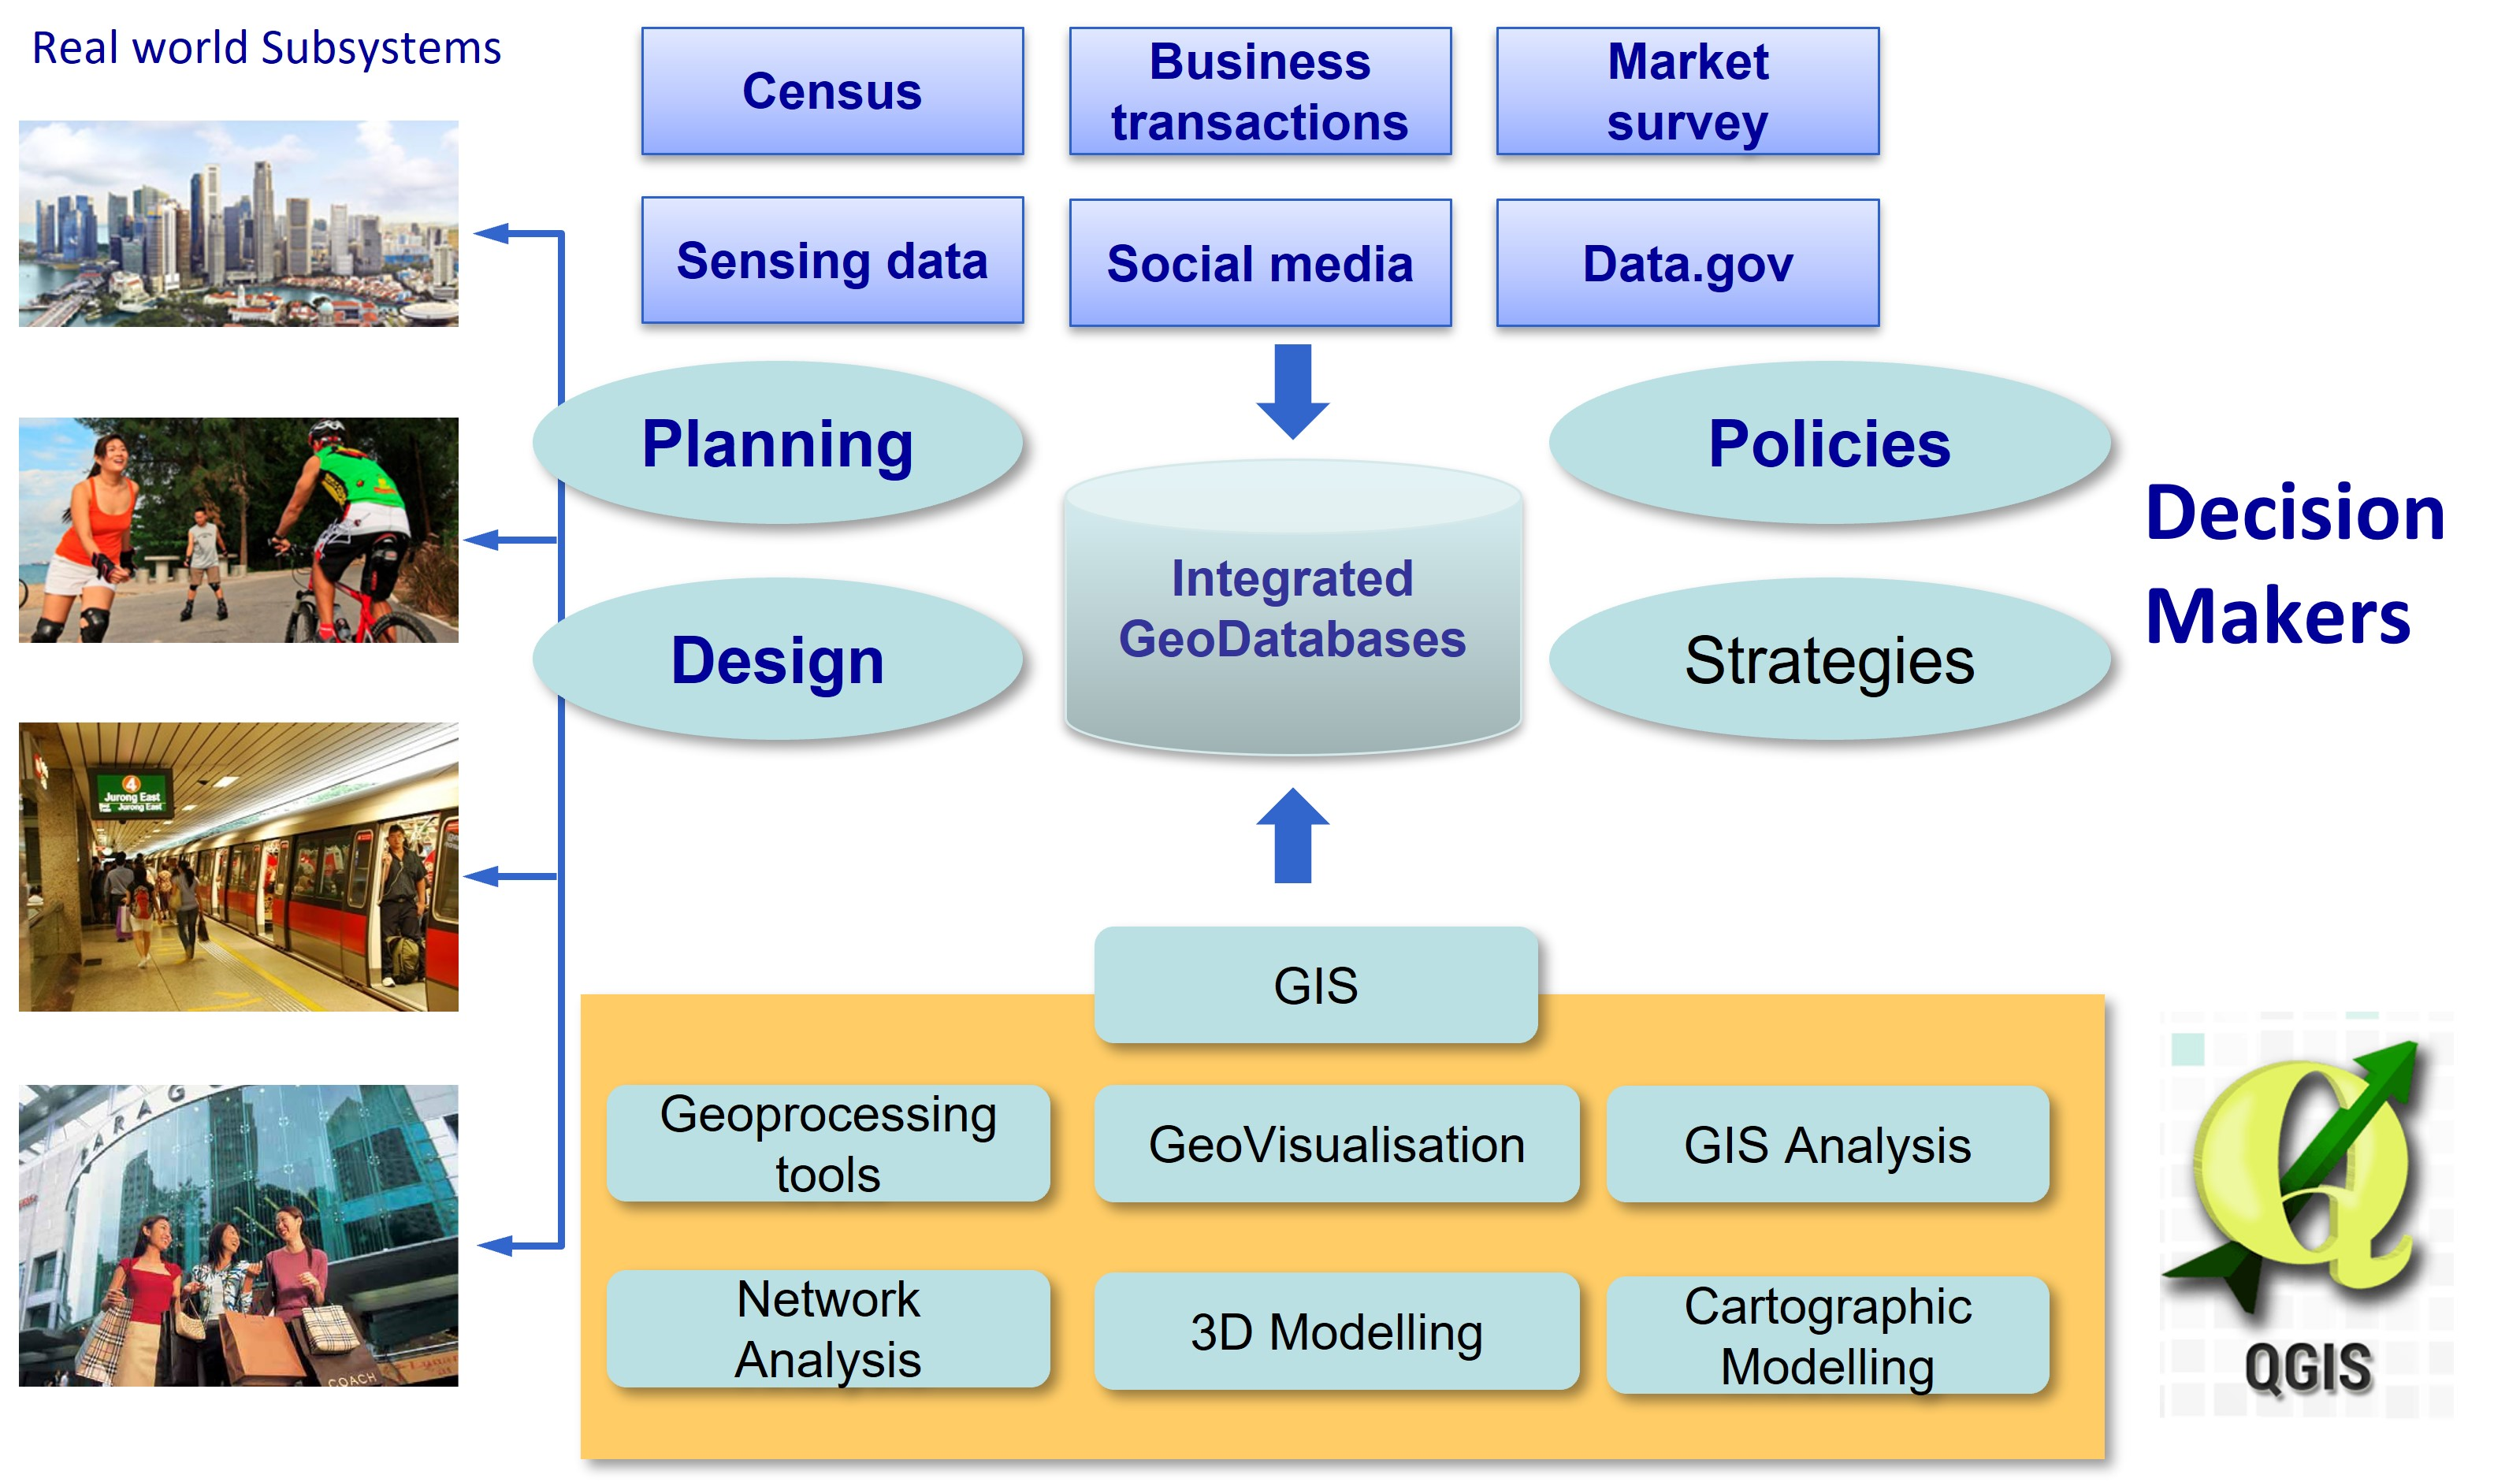
\includegraphics{./img/cover.jpg}

This workbook has two unique features. Firstly, all the exercises are
developed based on \href{https://www.qgis.org/en/site/}{QGIS}, an open
source GIS toolkit with full GIS functions including 3-D modelling,
Network Analysis and image analysis. Secondly, all the use cases and
data sets are from
\href{https://en.wikipedia.org/wiki/Singapore}{Singapore}, one of the
amazing city-state in the world with diverse culture.

\hypertarget{license}{%
\section*{License}\label{license}}
\addcontentsline{toc}{section}{License}

This website is (and will always be) \textbf{free to use}, and is
licensed under the
\href{https://creativecommons.org/licenses/by-nc-nd/4.0/}{Creative
Commons Attribution-NonCommercial-NoDerivs 4.0} License.

\bookmarksetup{startatroot}

\hypertarget{introduction}{%
\chapter{Introduction}\label{introduction}}

QGIS (formally known as Quantum GIS) is a full-features open source GIS
software. It is the GIS tool used in this course.

This section provides you with step-by-step guide on how to download and
install QGIS in your window-based computer (i.e.~desktop or laptop).

\hypertarget{downloading-qgis-installer}{%
\section{Downloading QGIS installer}\label{downloading-qgis-installer}}

\begin{itemize}
\item
  Launch the web browser.
\item
  In the address bar at the top of the window, enter http://qgis.org/
  and press \textbf{Enter}.
\end{itemize}

The website should look something like this:

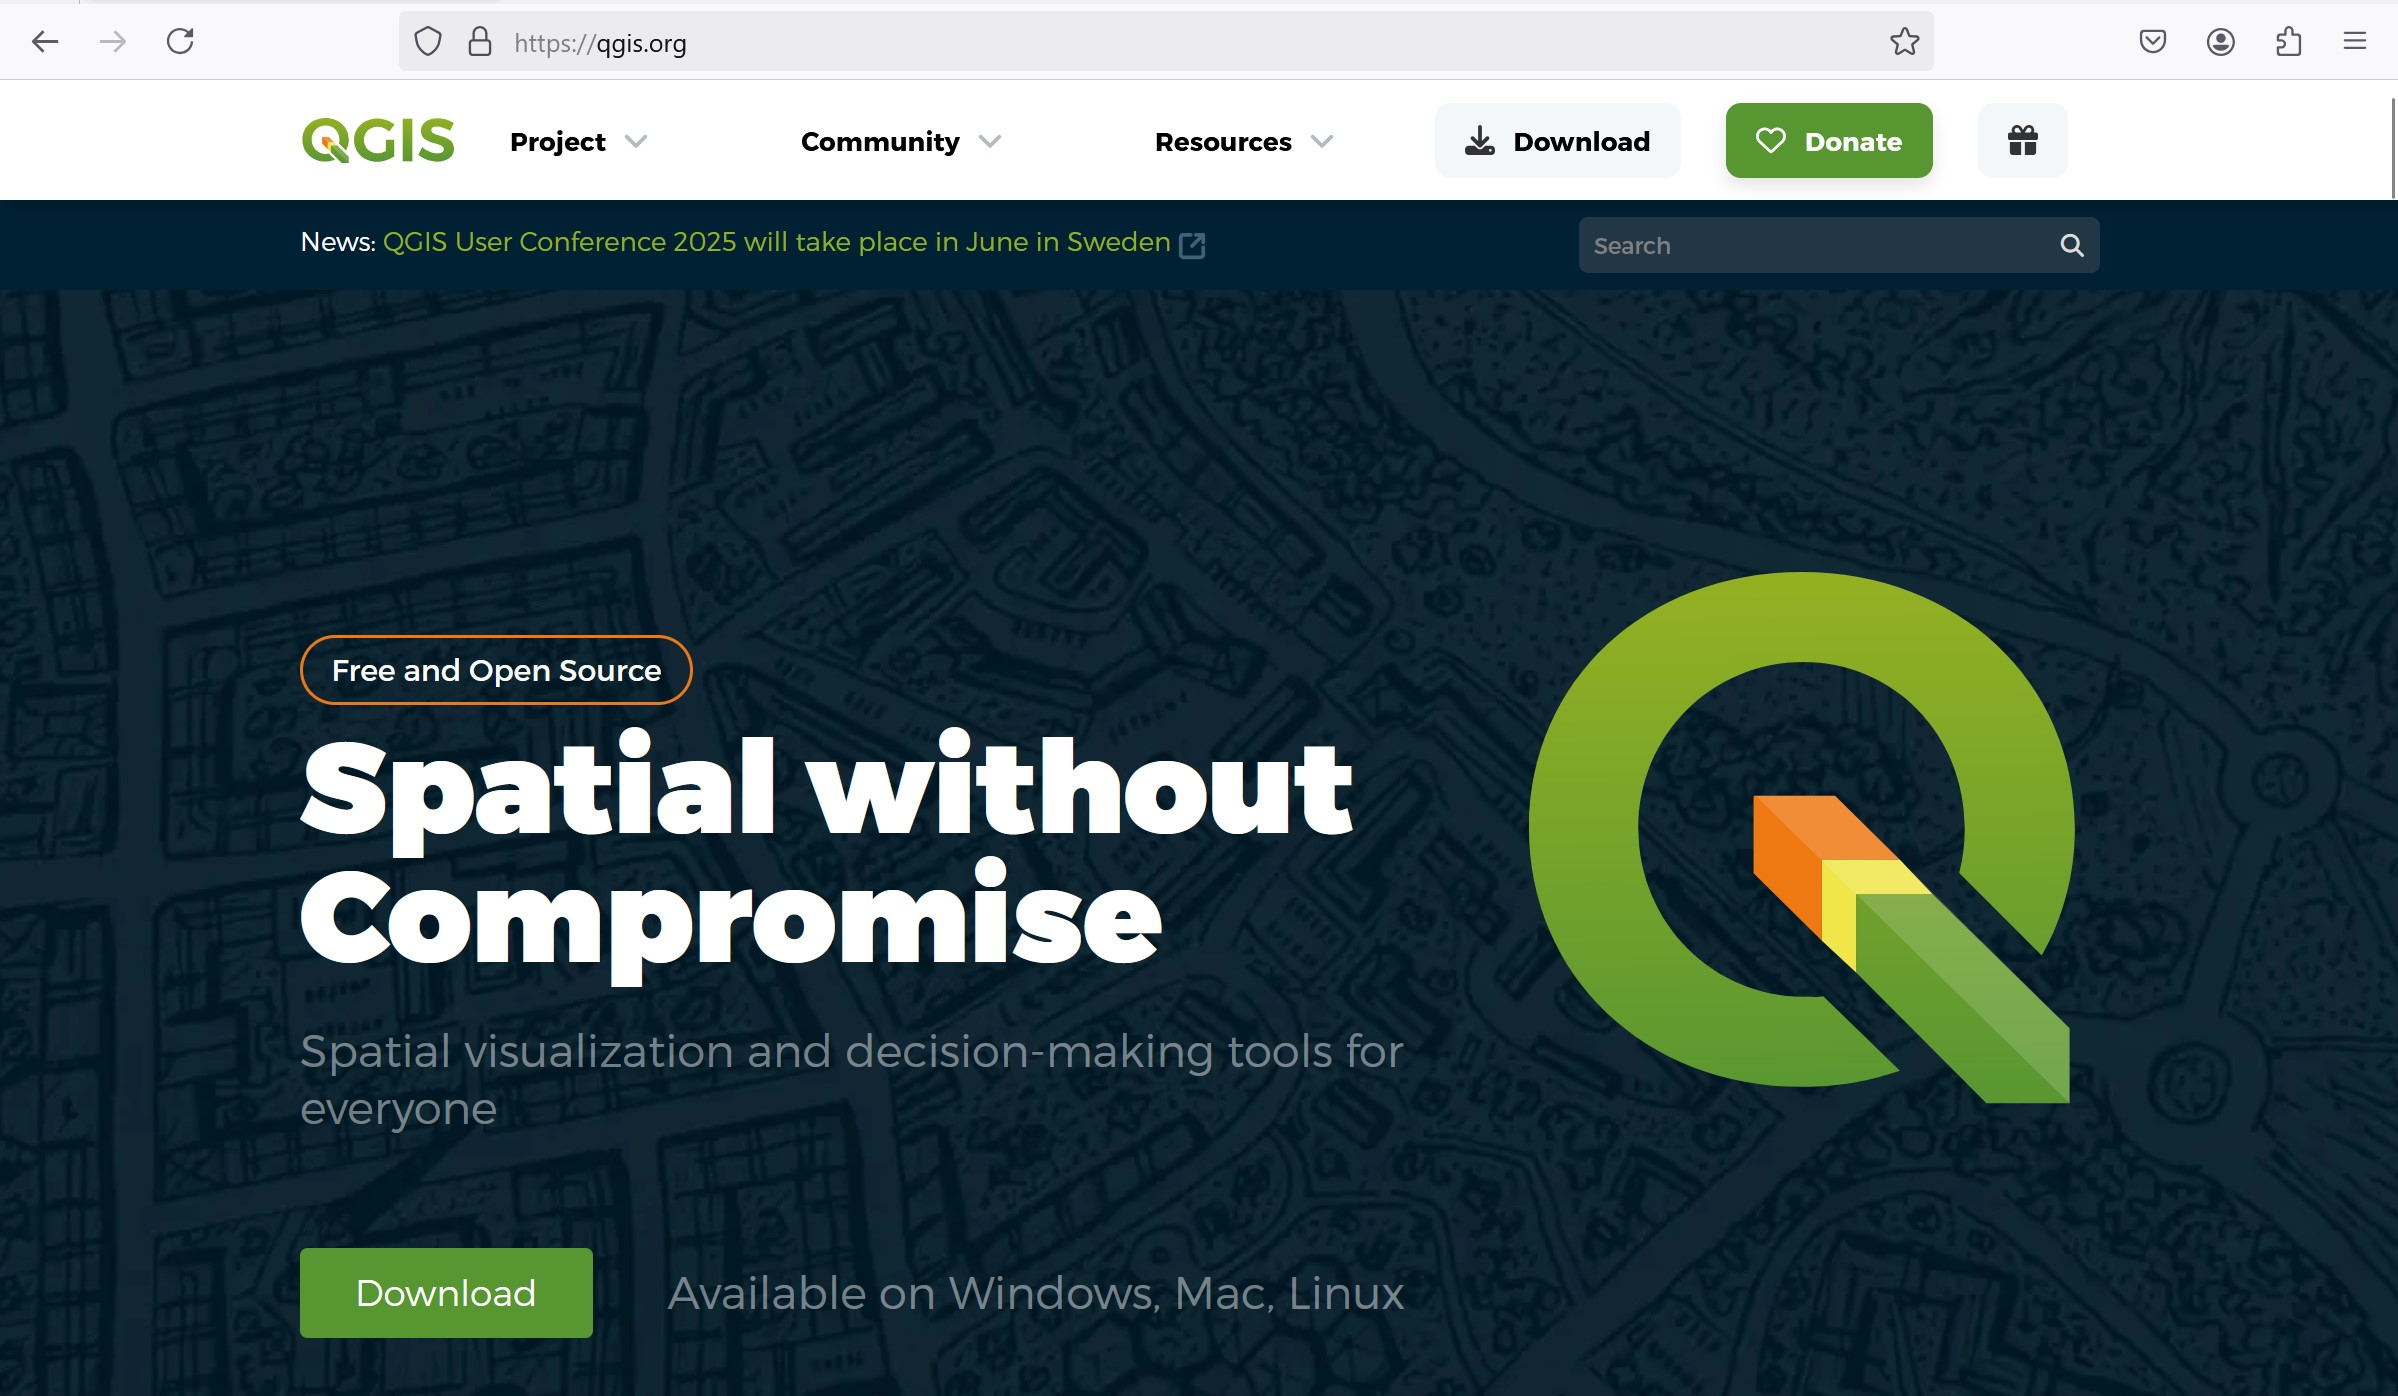
\includegraphics{./img/image1.jpg}

\begin{itemize}
\tightlist
\item
  Click on \textbf{Download Now} button.
\end{itemize}

Your screen should look similar to the figure below.

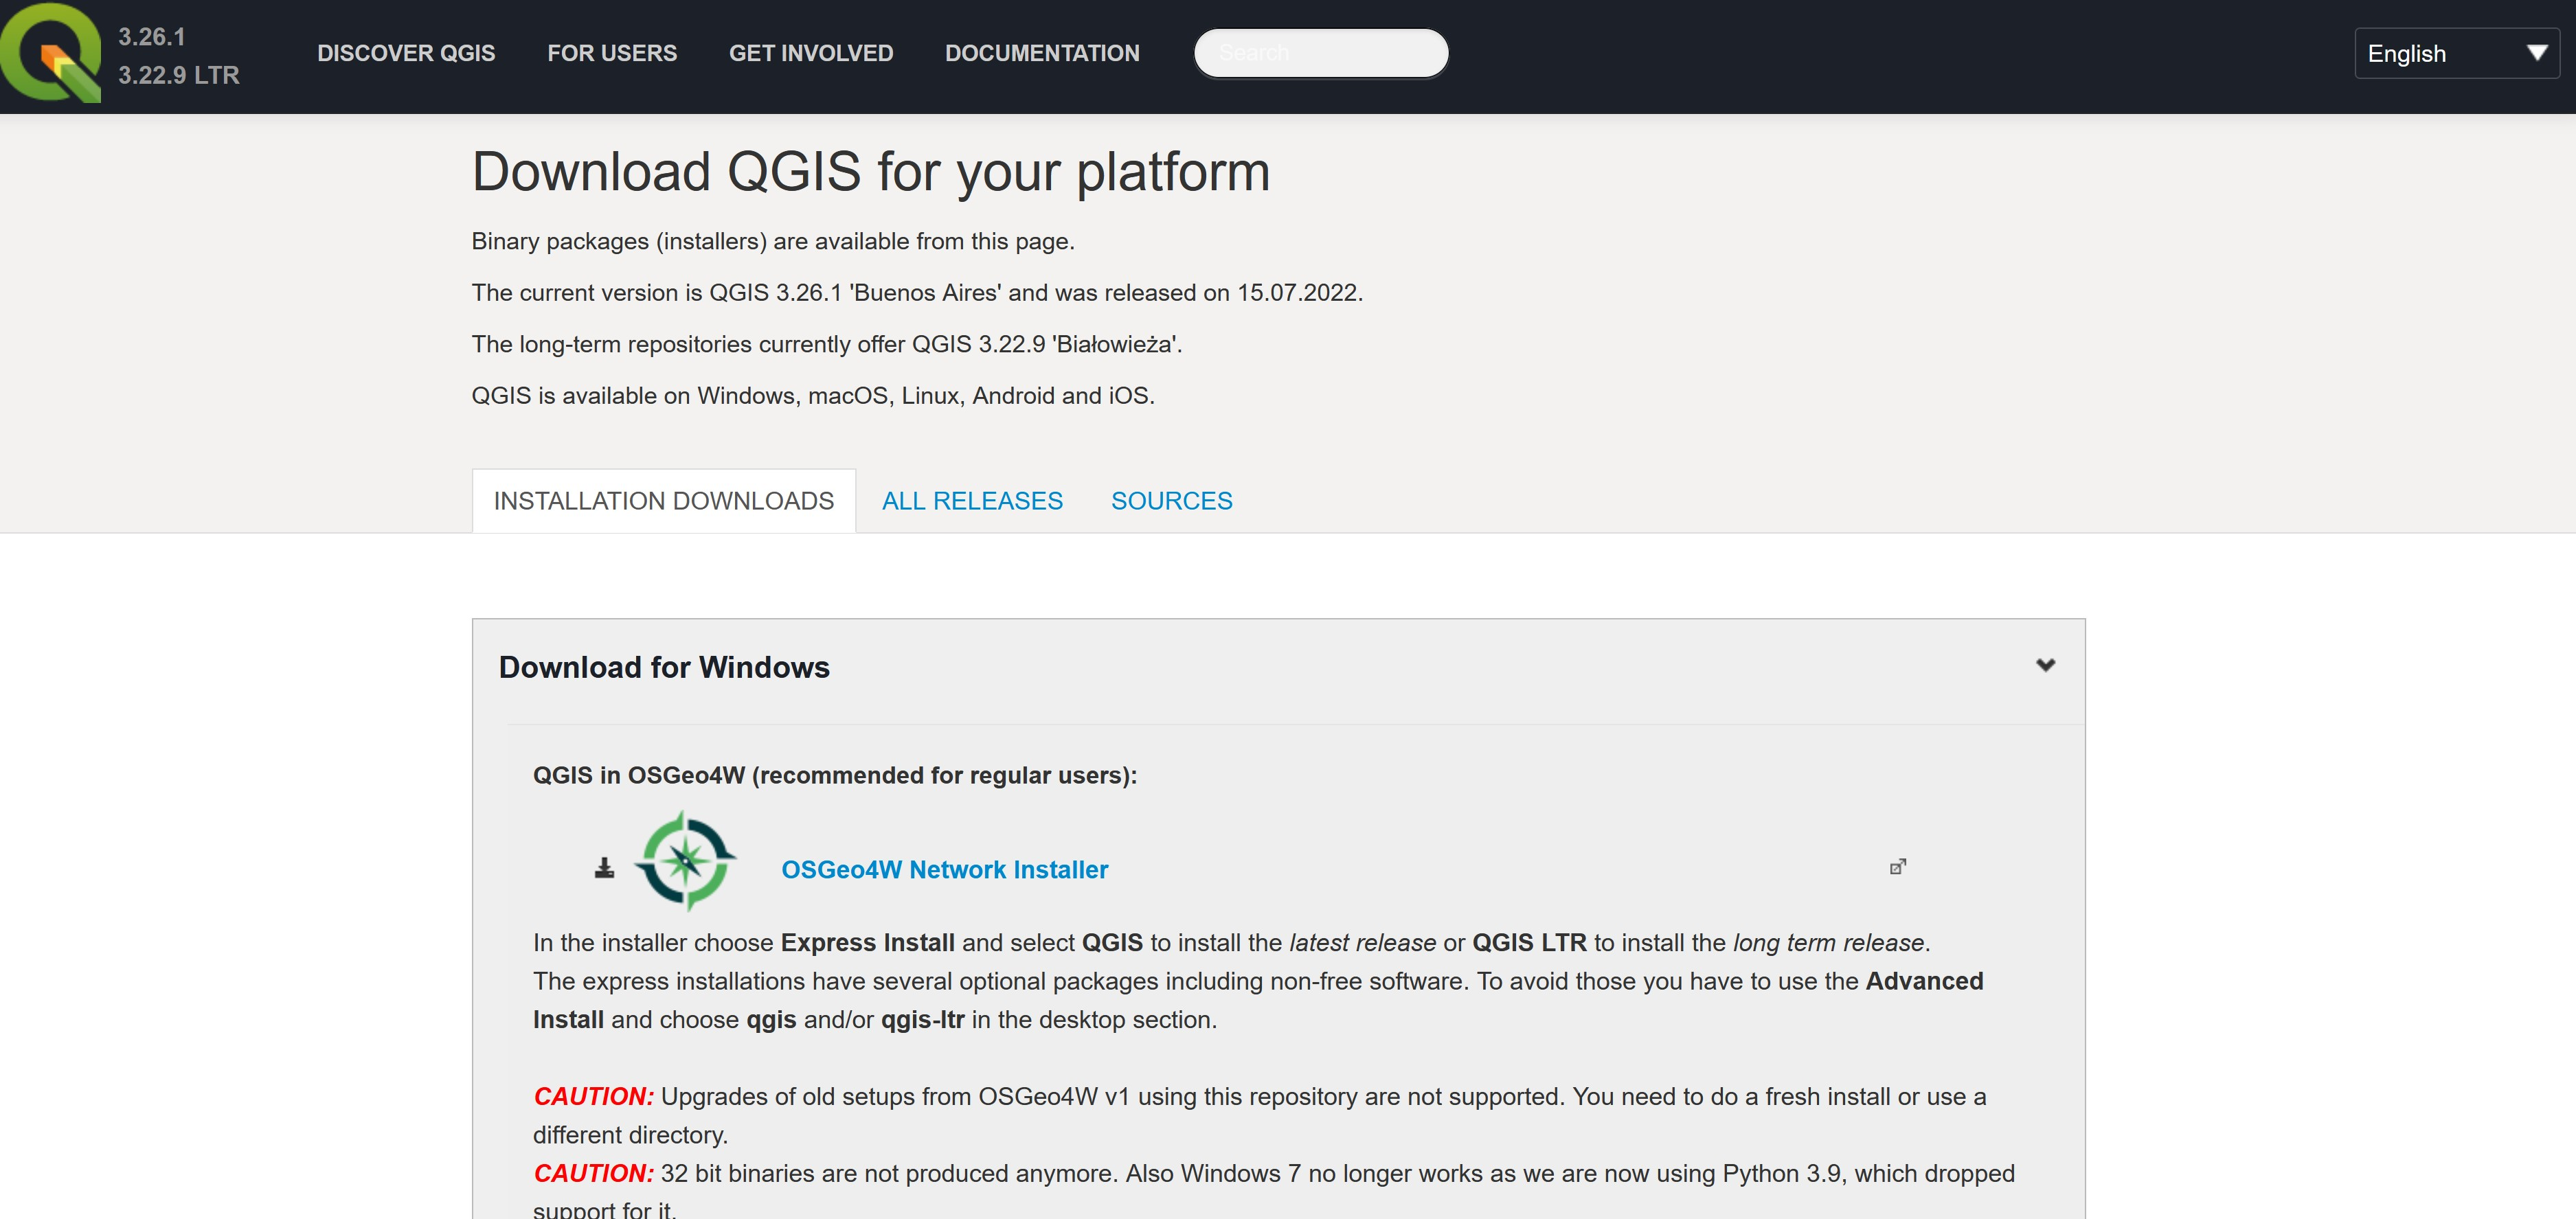
\includegraphics{./img/image2.jpg}

\begin{itemize}
\tightlist
\item
  Click on \textbf{QGIS Standalone Installer Version 3.26}
\end{itemize}

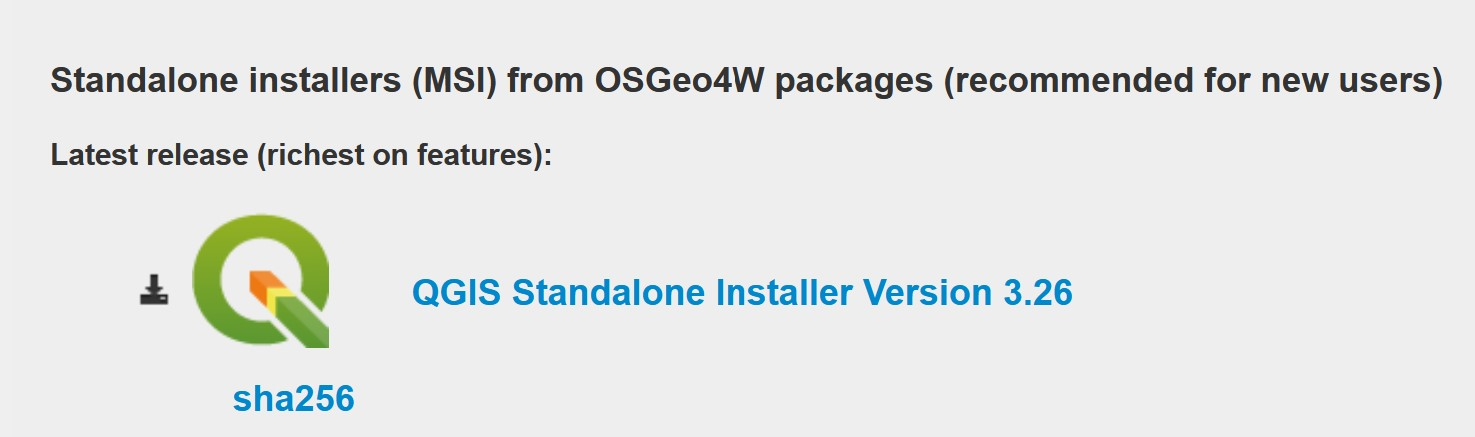
\includegraphics{./img/image3.jpg}

After a few seconds (depend on your network speed), a pop-up window
appears.

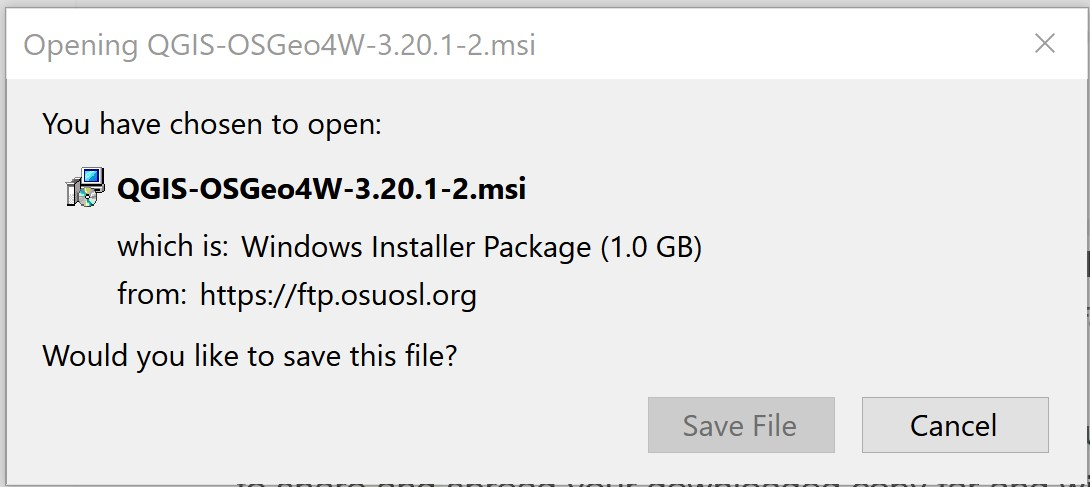
\includegraphics{./img/image4.jpg}

\begin{itemize}
\tightlist
\item
  Click on the \textbf{Save File} button.
\end{itemize}

Be patient, the downloading will take a few minutes depend on the speed
of your internet.

\hypertarget{installing-qgis}{%
\section{Installing QGIS}\label{installing-qgis}}

In this section, you will learn how to install QGIS into your computer.

\begin{itemize}
\item
  Find the QGIS installer on your computer, right-click and select
  \textbf{Install} from the context menu to launch the setup.
\item
  Click on the \textbf{Yes} button when Windows prompt you with the
  dialog ``Do you want to allow this app to make change to your
  device?''
\end{itemize}

After a few second, the Setup Wizard dialog window appears.

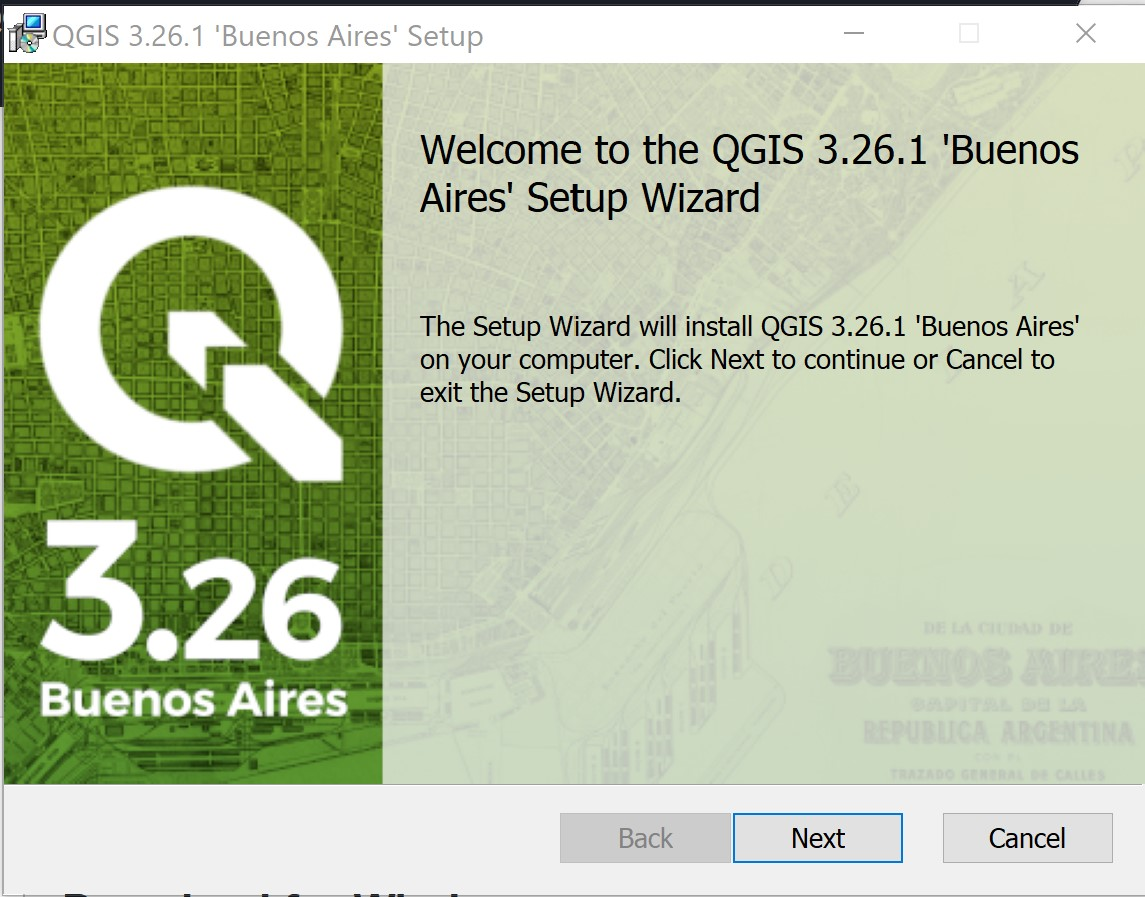
\includegraphics{./img/image5.jpg}

\begin{itemize}
\tightlist
\item
  Click on the \textbf{Next} button.
\end{itemize}

The End-User License Agreement dialog window appears.

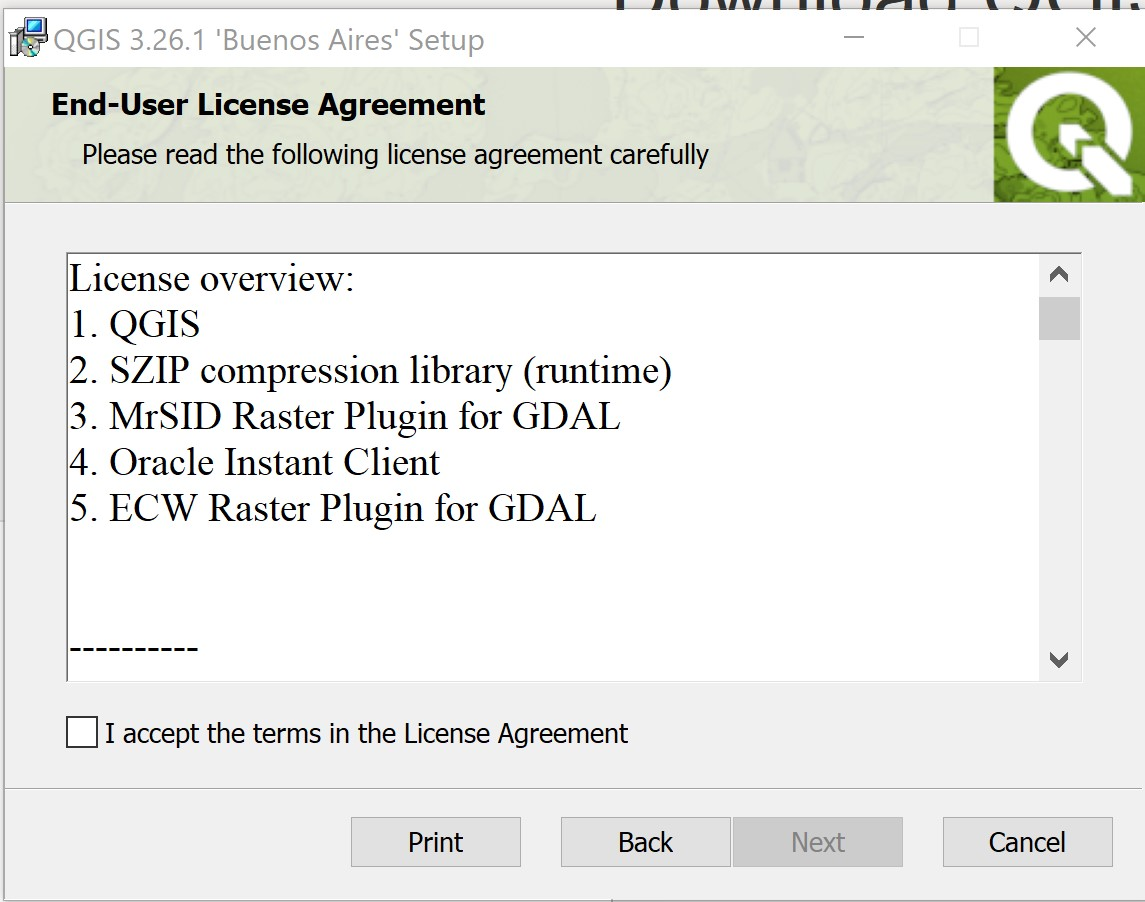
\includegraphics{./img/image6.jpg}

\begin{itemize}
\item
  Click on the checkbox in front of \textbf{I accept the terms in the
  License Agreement} button.
\item
  Then, click on \textbf{Next} button.
\end{itemize}

The Destination Folder dialog window appears.

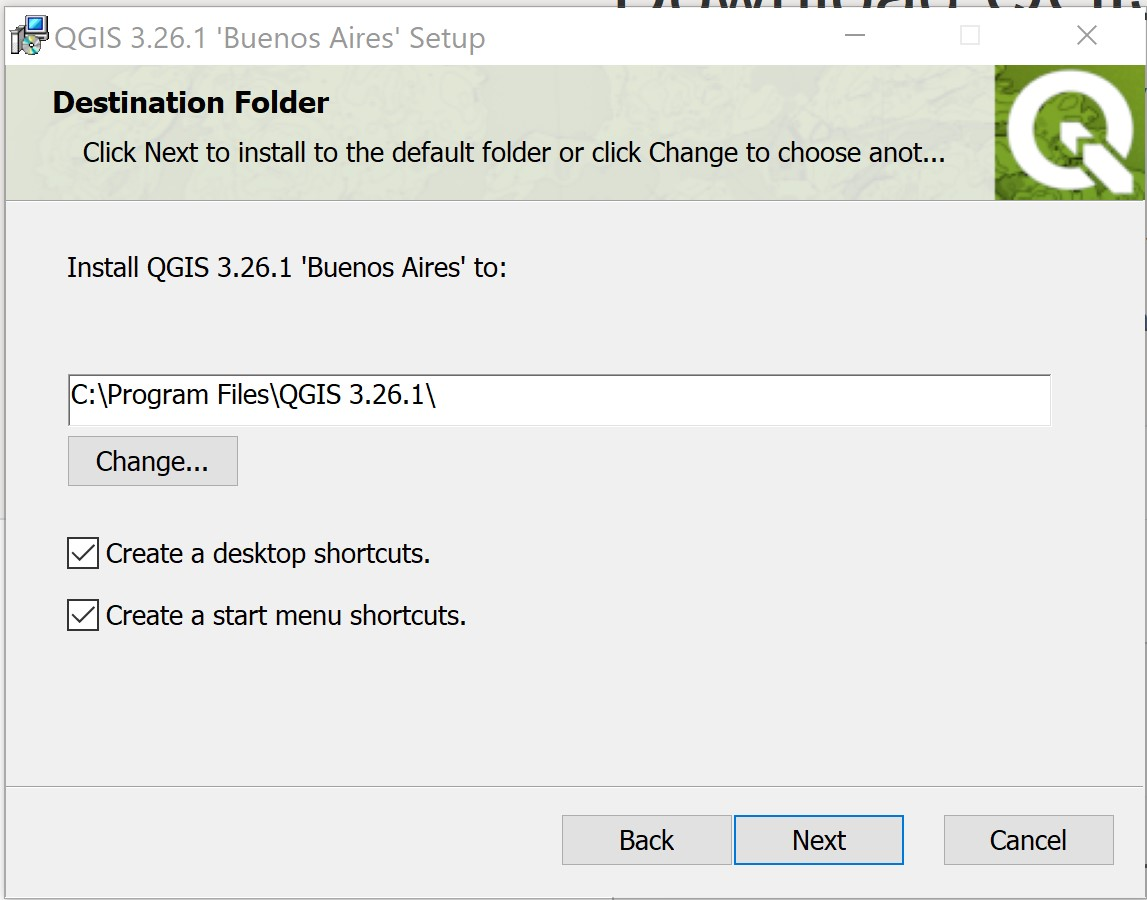
\includegraphics{./img/image7.jpg}

\begin{itemize}
\item
  Ensure that the Destination Folder is at
  \texttt{C:\textbackslash{}Program\ Files\textbackslash{}QGIS\ 3.26.1\textbackslash{}}
\item
  Keep both checkboxes selected.
\item
  Click on the \textbf{Next} button.
\end{itemize}

The \textbf{Ready to install QGIS 3.26.1 `Buenos Aires'} dialog window
appears.

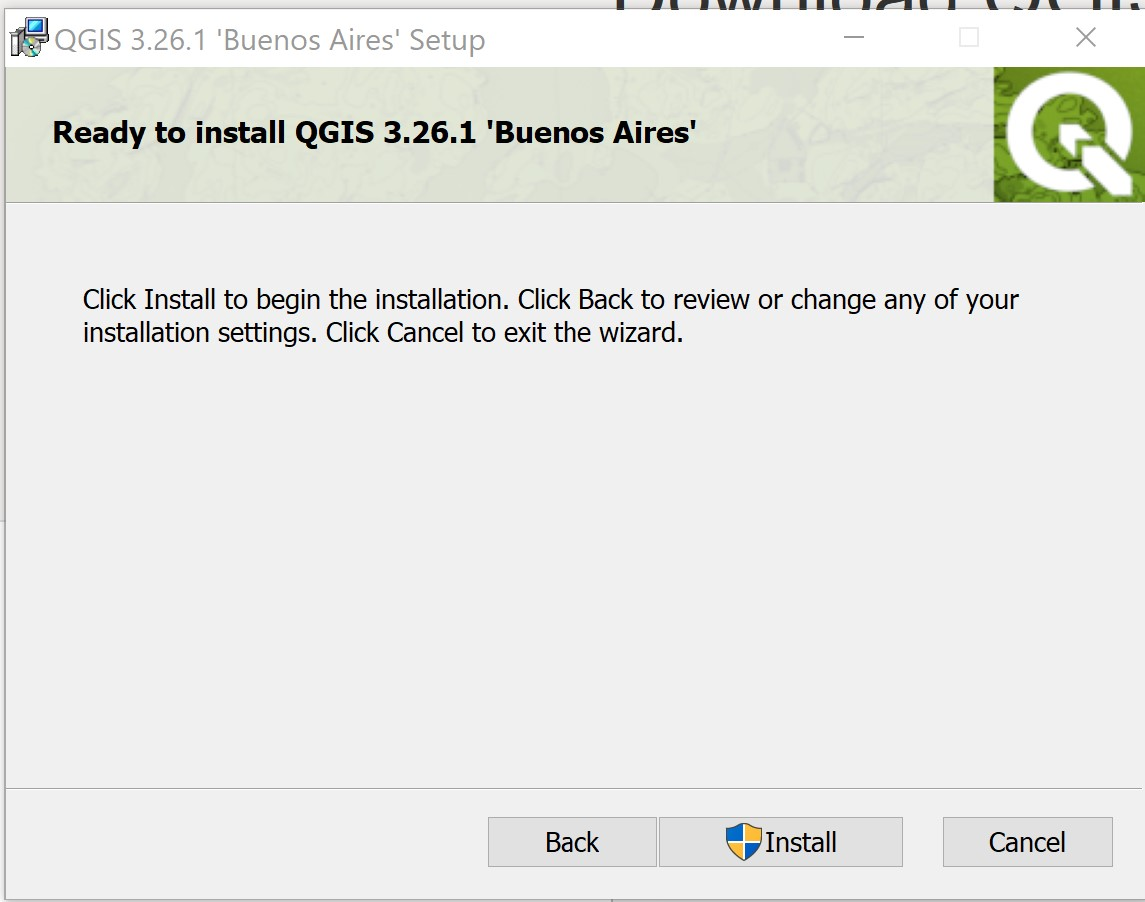
\includegraphics{./img/image8.jpg}

\begin{itemize}
\tightlist
\item
  Click on \textbf{Install} button to start the installation process.
\end{itemize}

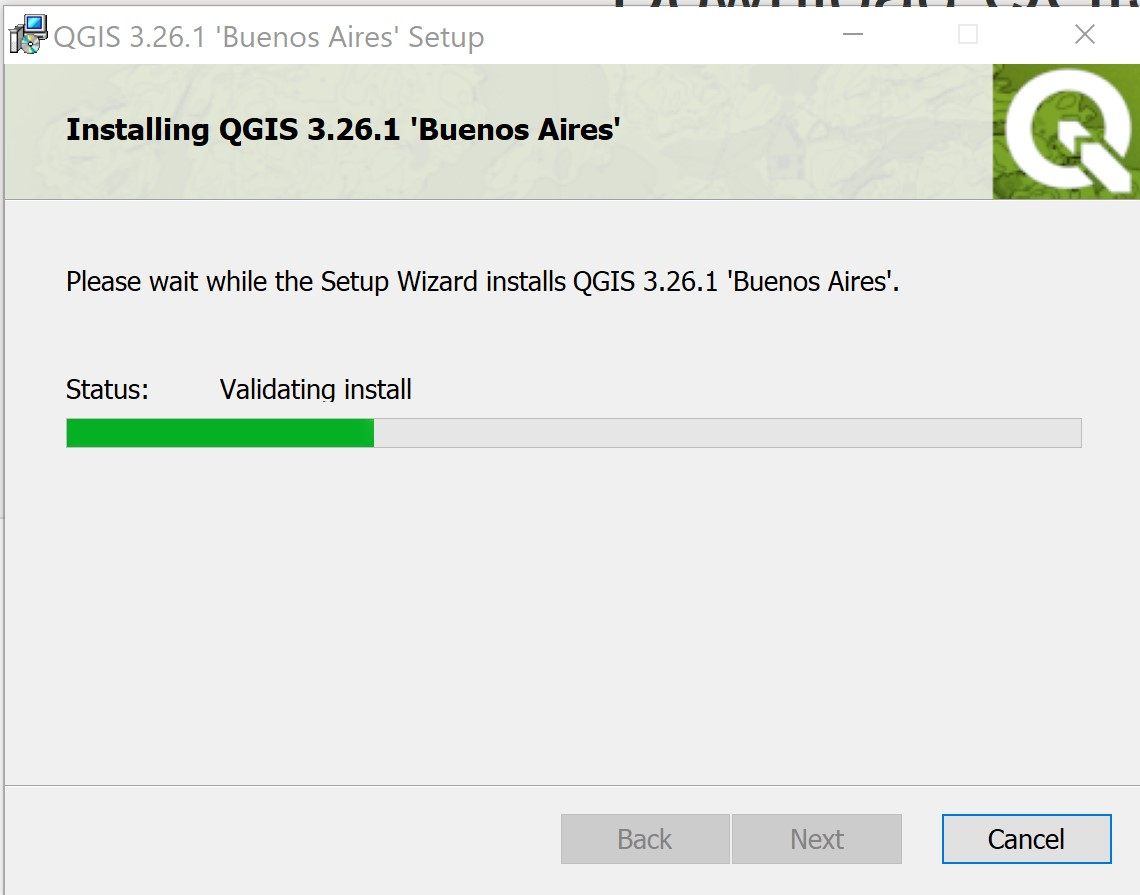
\includegraphics{./img/image9.jpg}

QGIS will begin to install. It may take a few minutes to install so be
patient.

When the installation is completed, a Setup Wizard window look similar
to the screenshot below appears.

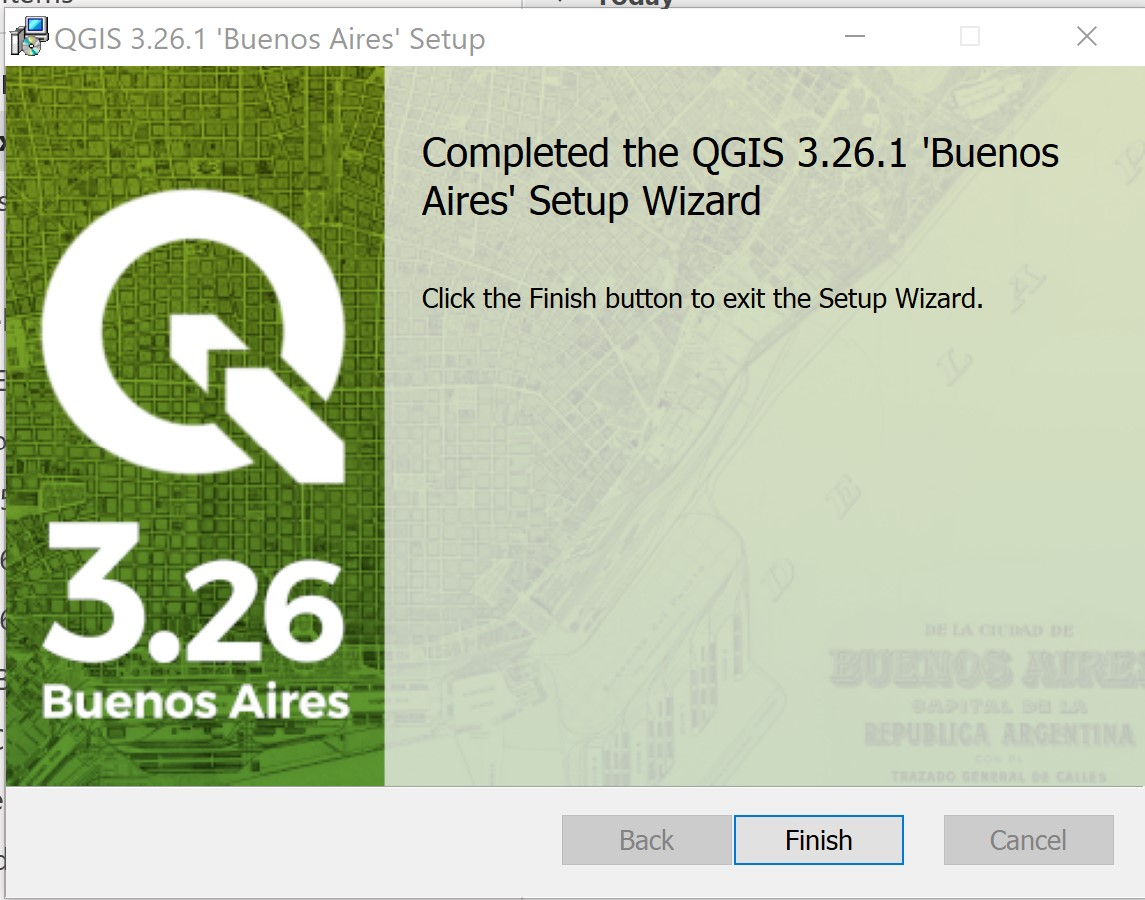
\includegraphics{./img/image10.jpg}

\begin{itemize}
\tightlist
\item
  Click on \textbf{Finish} button.
\end{itemize}

Congratulations! You have installed QGIS successfully!

\bookmarksetup{startatroot}

\hypertarget{my-first-date-with-qgis}{%
\chapter{My First Date with QGIS}\label{my-first-date-with-qgis}}

In this hands-on exercise, you will learn the basic operations of a GIS
software in general and the graphic user interfaces (GUIs) of QGIS
specifically.

\hypertarget{getting-started}{%
\section{Getting Started}\label{getting-started}}

First, you will launch QGIS.

\begin{itemize}
\tightlist
\item
  At your window desktop, double-click on \textbf{QGIS Desktop3.26}
  icon.
\end{itemize}

After a few seconds, QGIS window appears.

\begin{itemize}
\tightlist
\item
  On the \emph{QGIS Tips! Dialog} window, click on the \textbf{OK}
  button.
\end{itemize}

Your screen should look similar to the figure below.

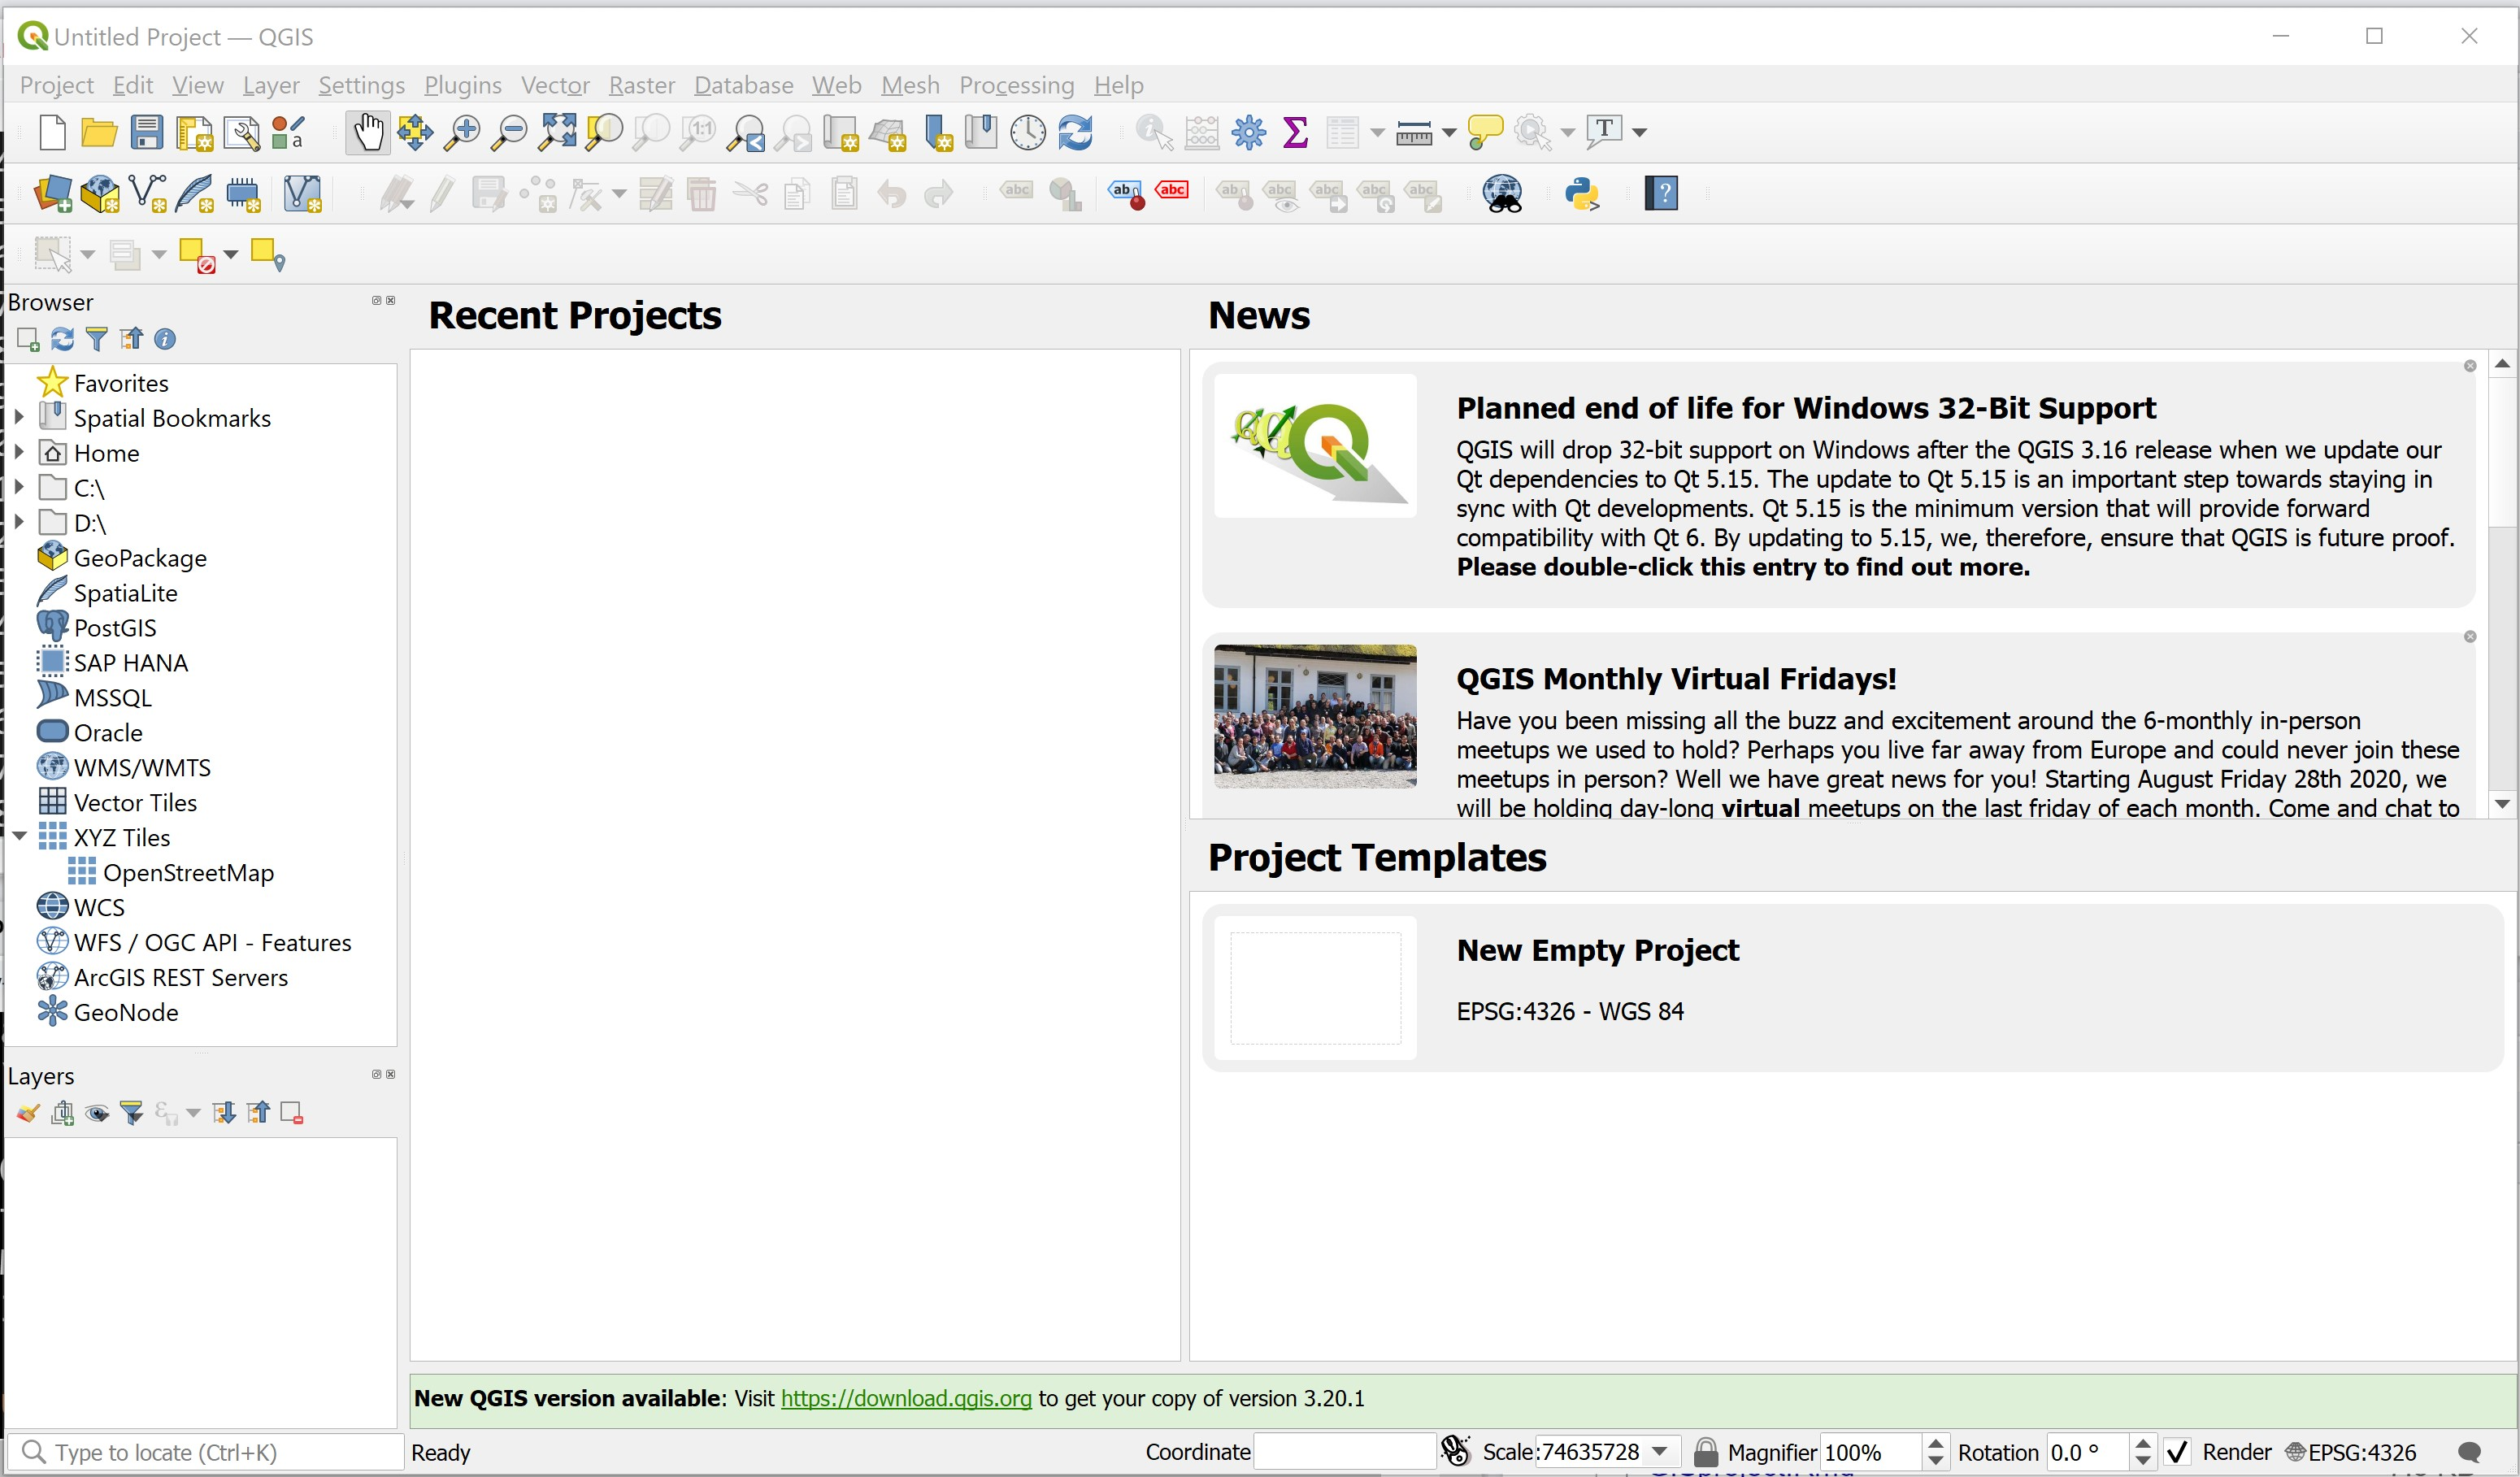
\includegraphics{./img/image1-5.jpg}

\hypertarget{getting-to-know-a-gis-project-file}{%
\subsection{Getting to know a GIS project
file}\label{getting-to-know-a-gis-project-file}}

A GIS project file provides a link between the GIS software and the
geospatial datasets instead of stored data. It also contains GIS
operation configurations such as symbolisation used, data
classification, map projection, the paths of each data and map design.
In this section, you will explore an existing QGIS's project file called
Hands-on01.qgs.

\begin{itemize}
\tightlist
\item
  Start Window Explorer.
\item
  Navigate to
  \texttt{\textbackslash{}SMT201\textbackslash{}Hands-on\_Ex01\textbackslash{}}
  sub-folder.
\end{itemize}

You will find a file called \texttt{Hands-On01.qgs} in the sub-folder.

\begin{itemize}
\tightlist
\item
  Right-click on \texttt{Hands-On01.qgs}.
\item
  Select \textbf{Open} with from the context menu.
\item
  Use the \textbf{Notepad} to open the file.
\end{itemize}

The Notedpad window should look similar to the figure below.

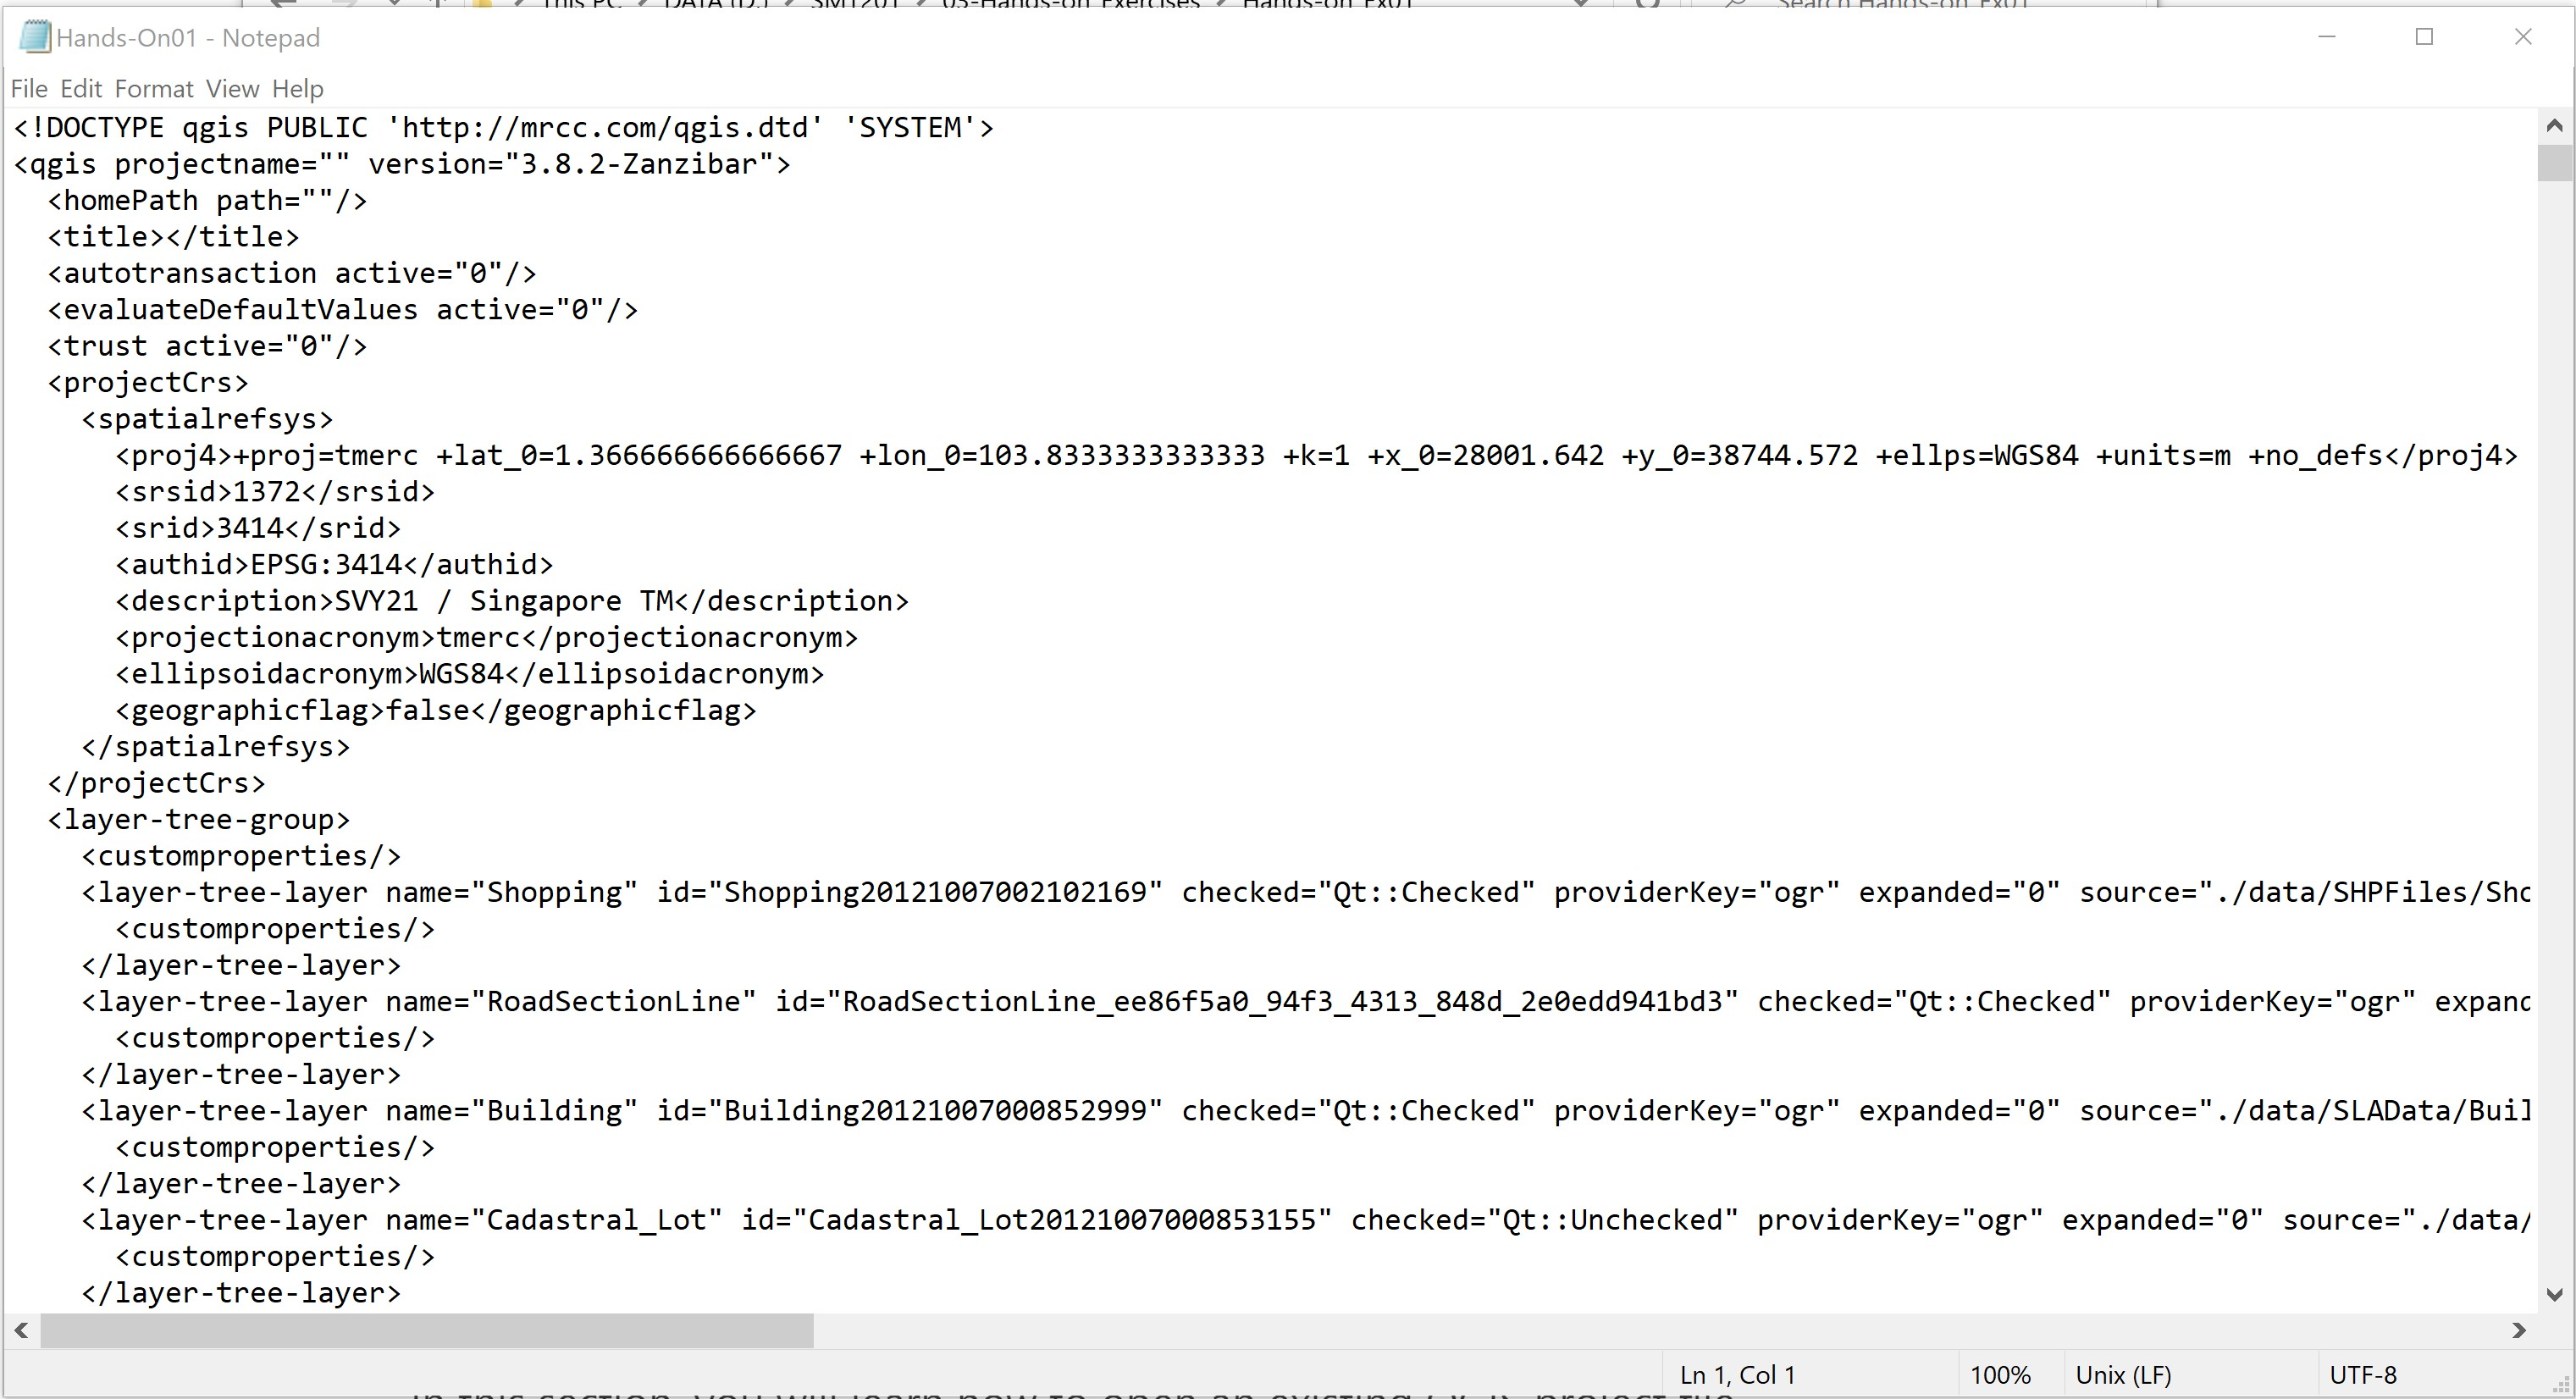
\includegraphics{./img/image1-6.jpg}

Notice that the QGIS project file is actually in XML format.

\begin{itemize}
\tightlist
\item
  Close Notepad.
\end{itemize}

\hypertarget{open-an-existing-project-file}{%
\subsection{Open an existing project
file}\label{open-an-existing-project-file}}

In this section, you will learn how to open an existing QGIS project
file.

\begin{itemize}
\tightlist
\item
  From QGIS main menu, click on \textbf{Project} -\textgreater{}
  \textbf{Open}.
\end{itemize}

The \texttt{Choose\ a\ QGIS\ project\ file\ to\ open} dialog window
appears.

\begin{itemize}
\tightlist
\item
  Navigate to
  \texttt{\textbackslash{}SMT201\textbackslash{}Hands-on\_Ex01\textbackslash{}}
  sub-folder.
\item
  Double-click on \texttt{Hans-On01.qgs} file.
\end{itemize}

Your screen should look similar to the figure below.

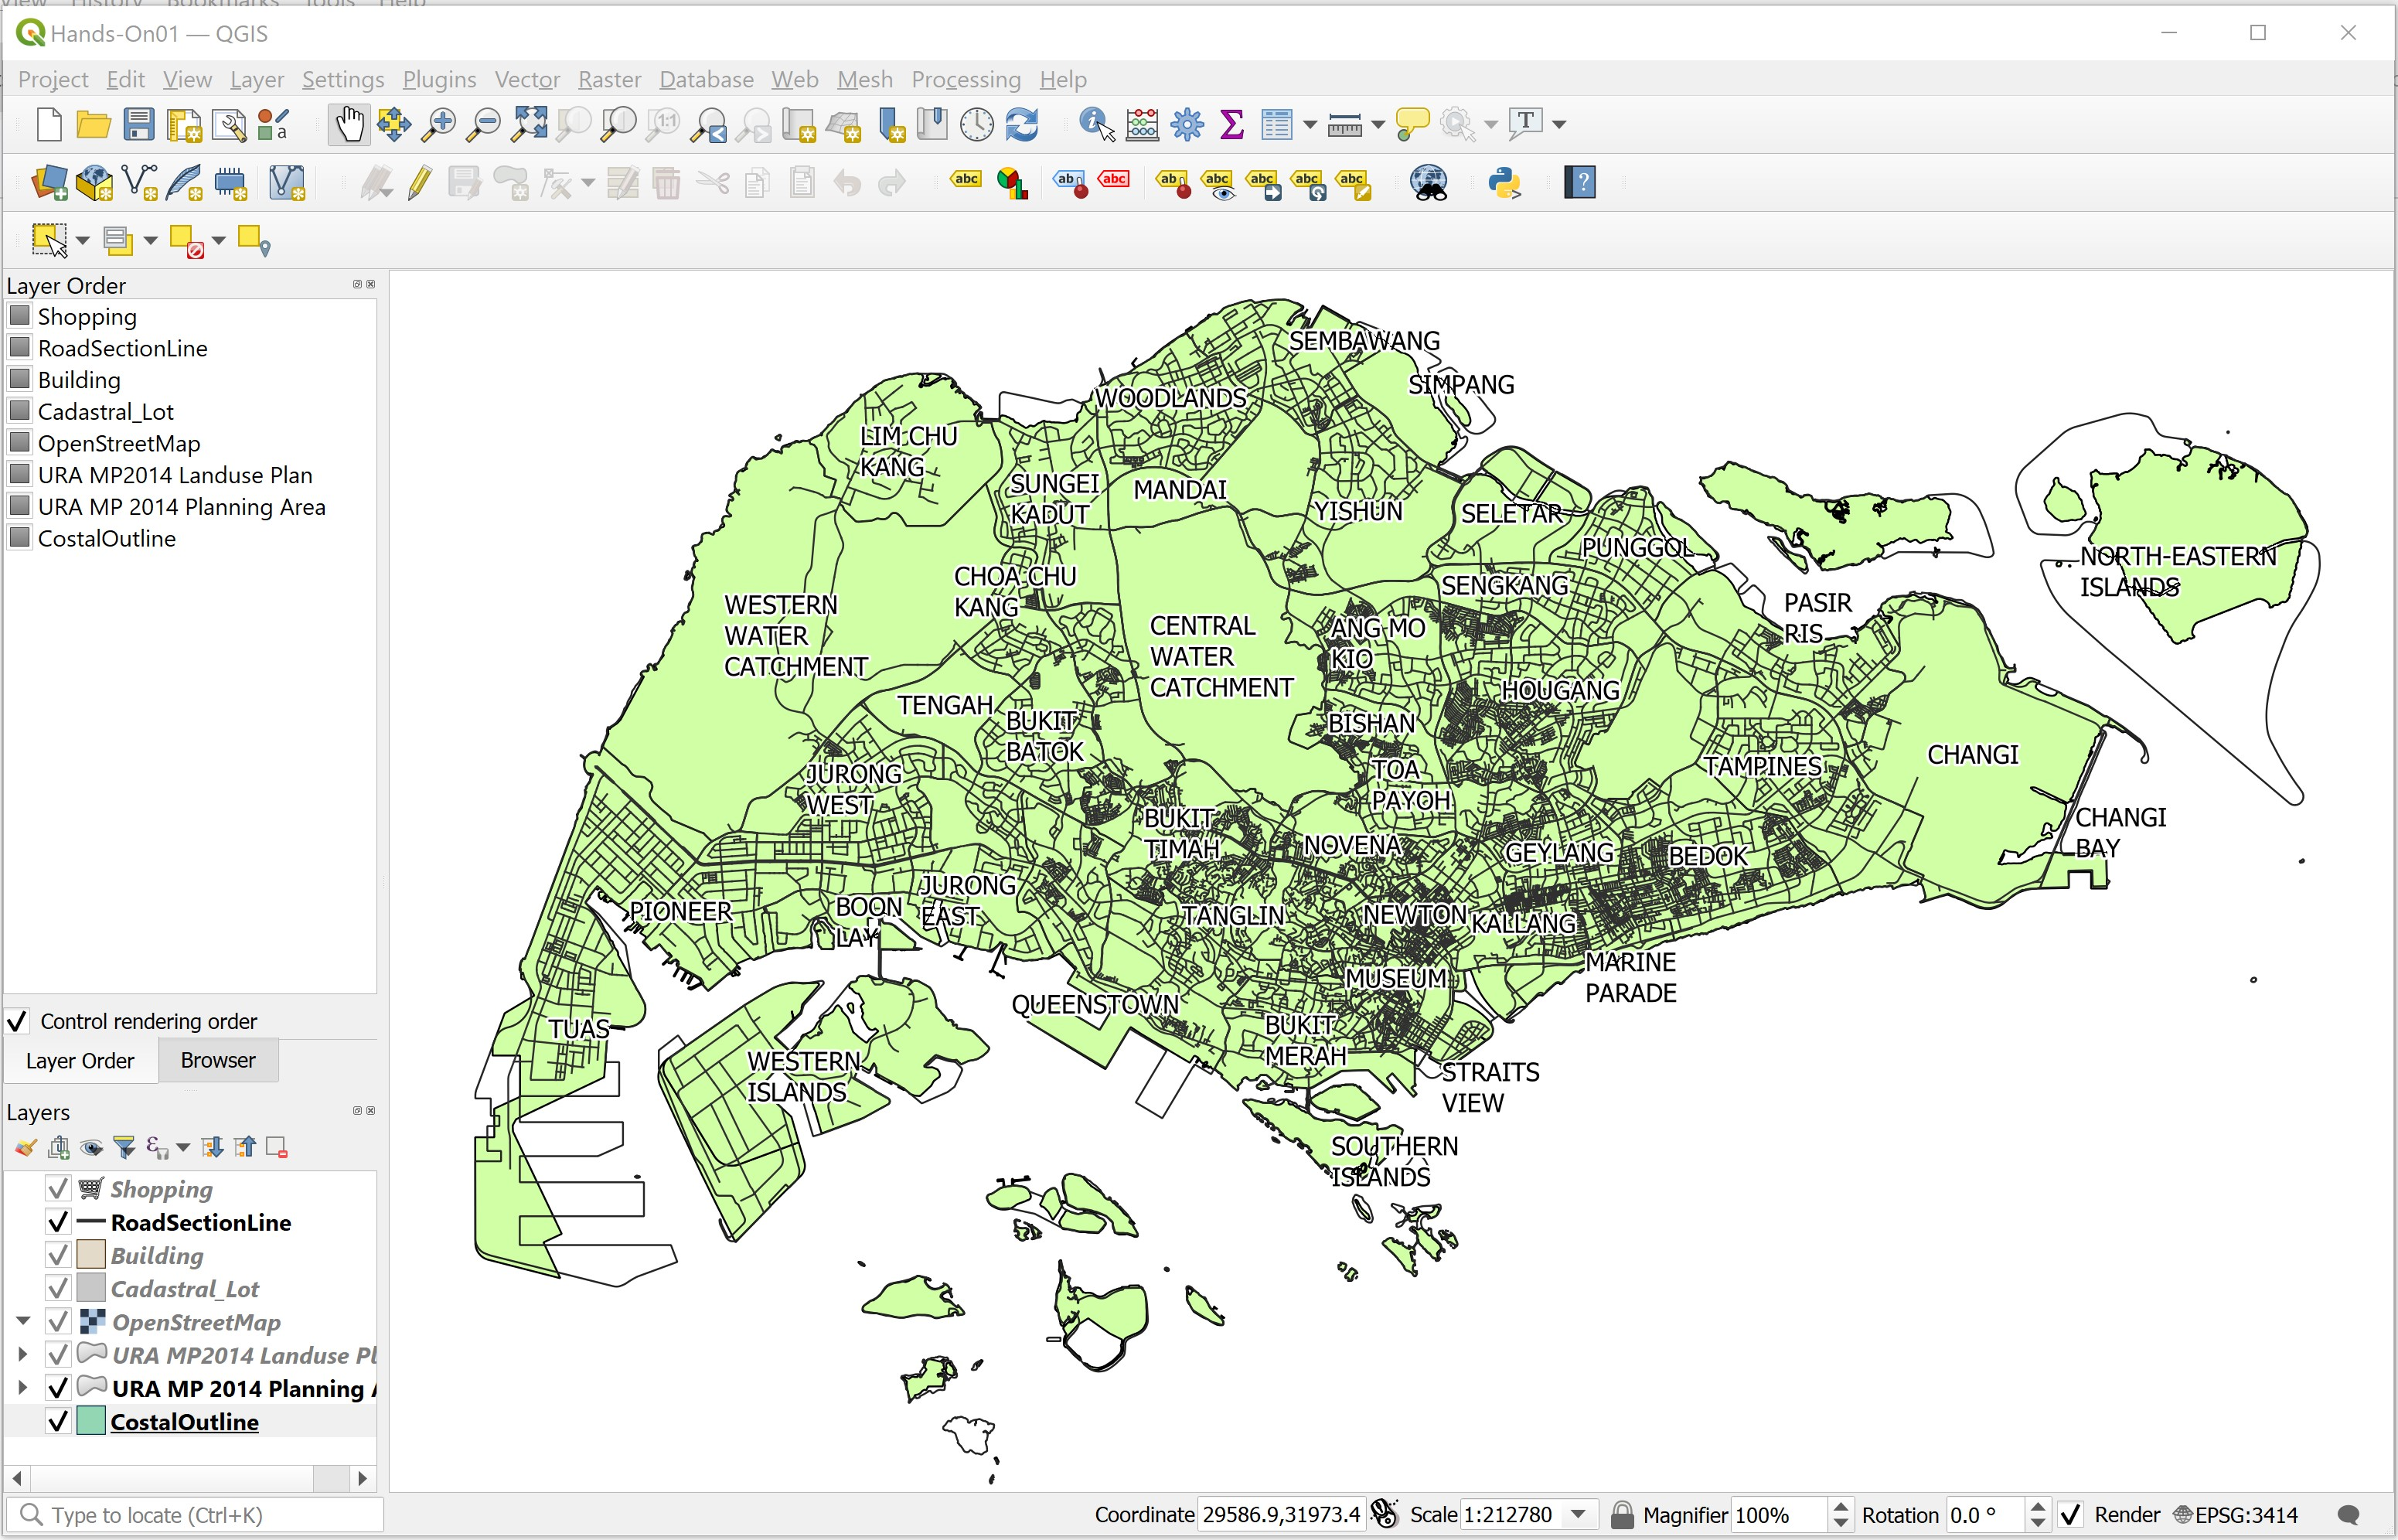
\includegraphics{./img/image1-7.jpg}

\hypertarget{exploring-qgis-interfaces}{%
\section{Exploring QGIS interfaces}\label{exploring-qgis-interfaces}}

The QGIS interface comprises six major components. They are: menu bar,
toolbar, map legend, browser, status bar and map view. The \textbf{Menu
Bar} provides access to various features and functions of QGIS using
hierarchical menu. The location of the menu and menu items is fixed,
although if you activate certain plugins, they may add an additional
menu to the bar.

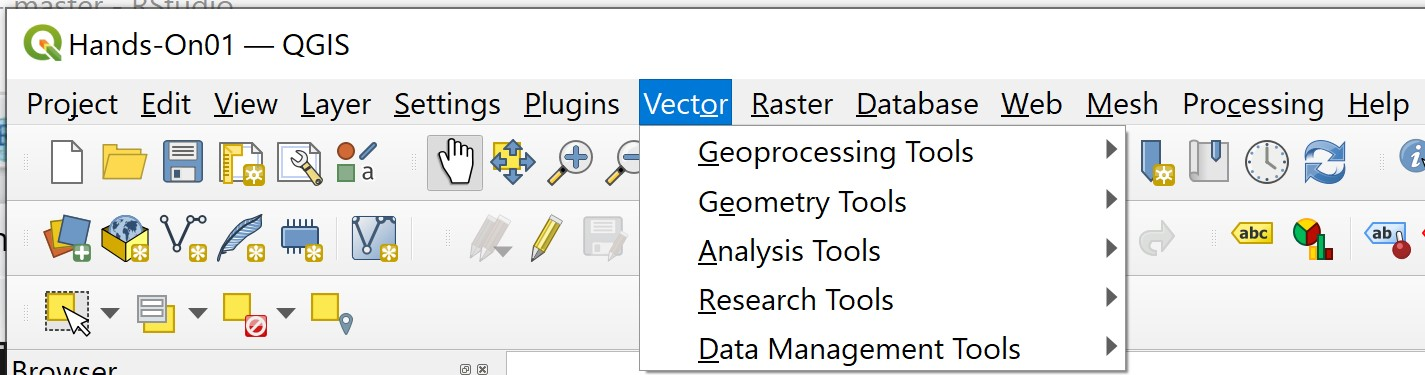
\includegraphics{./img/image1-8.jpg}

The \textbf{Toolbar} replicates many of the features and functions in
the Menu Bar, providing access to common features in a single click. The
location of the toolbar is not fixed; if you hover over the edge of the
toolbar and hold down the left mouse button you can drag the toolbar
wherever you like.

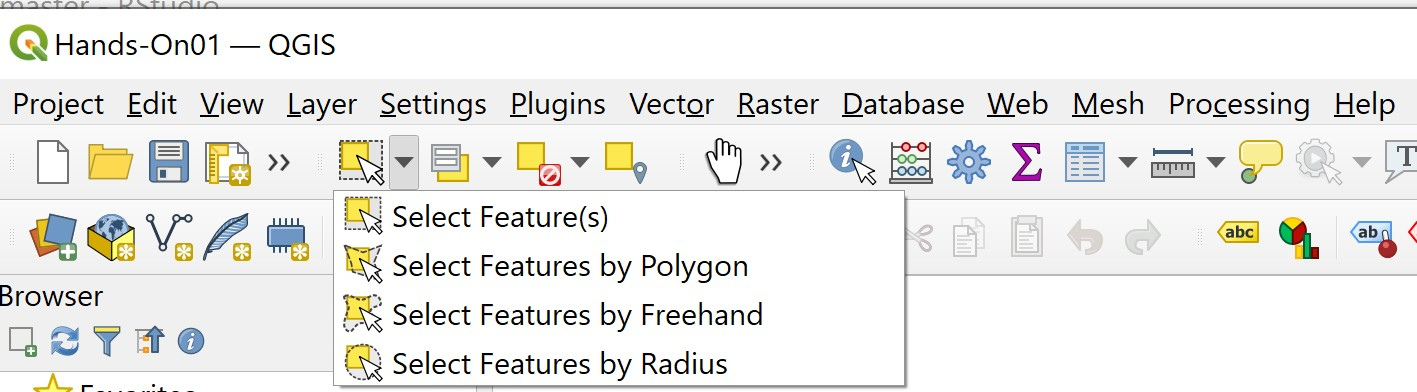
\includegraphics{./img/image1-9.jpg}

The \textbf{Map Legend} lists data layers that are linked with the
current project.

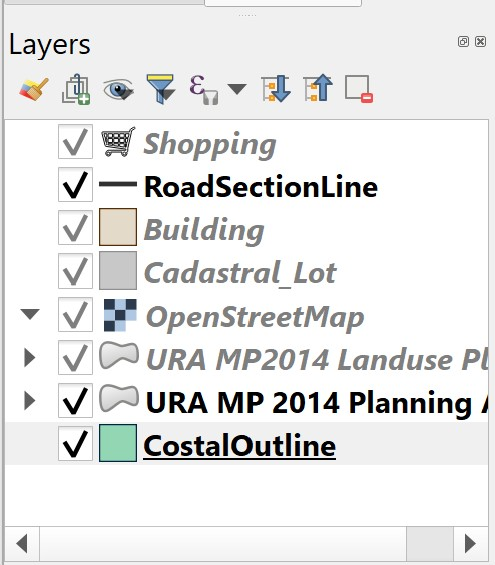
\includegraphics[width=0.3\textwidth,height=\textheight]{./img/image1-10.jpg}

You can turn each of the data layer on and off by clicking on the
checkbox in front of each data layer.

\begin{itemize}
\tightlist
\item
  From the Map Legend, click on the checkbox in front of CoastalOutline.
\end{itemize}

Notice that the Singapore boundary map on the Map View window
disappears.

\begin{itemize}
\tightlist
\item
  Click on the checkbox in front of CoastalOutline again.
\end{itemize}

Notice that the Singapore boundary map on the Map View window
re-appears.

The \textbf{Browser}, a new feature in QGIS 2.0, allows users to see
their file system and all of the GIS data files and databases. It also
allows users to drag files from the file system into QGIS project.

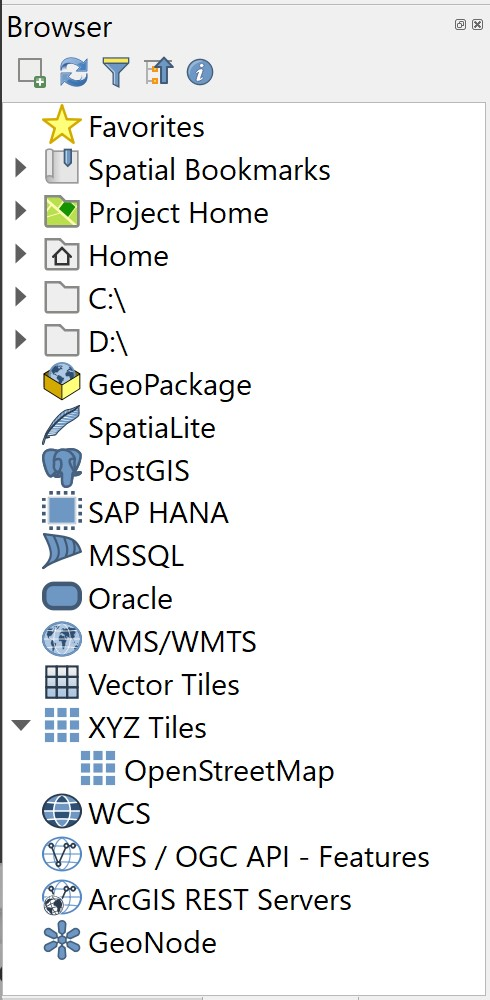
\includegraphics[width=0.3\textwidth,height=\textheight]{./img/image1-11.jpg}

The \textbf{Status Bar} shows the current scale of the map view, the
coordinates of the current position of the cursor and the coordinate
system used by the project. When a computation operation such as
buffering is used, the progress meters will appear here to show the
progress of the operations.

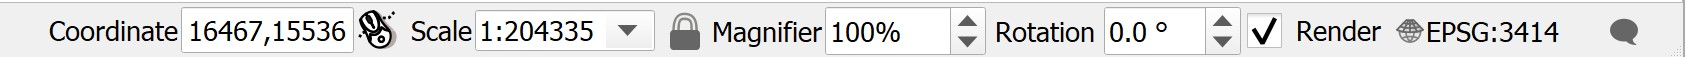
\includegraphics{./img/image1-12.jpg}

Last but not least, the \textbf{Map View} window displays all the active
layers in the project.

\hypertarget{navigating-the-map-view}{%
\section{Navigating the Map View}\label{navigating-the-map-view}}

\hypertarget{navigating-around-a-gis-view}{%
\subsection{Navigating around a GIS
view}\label{navigating-around-a-gis-view}}

In this section, you will learn how to navigate around the Map View.
First, you will work with the navigation tools.

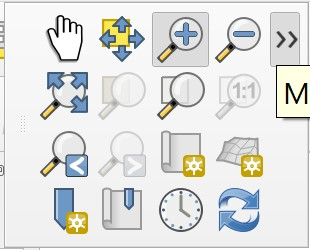
\includegraphics[width=0.3\textwidth,height=\textheight]{./img/image1-13.jpg}

\begin{itemize}
\tightlist
\item
  From the \textbf{Toolbar}, click on the \textbf{Zoom In} tool.
\item
  Hover the mouse to the centre of Singapore, click once.
\end{itemize}

Your screen should look similar to the figure below.

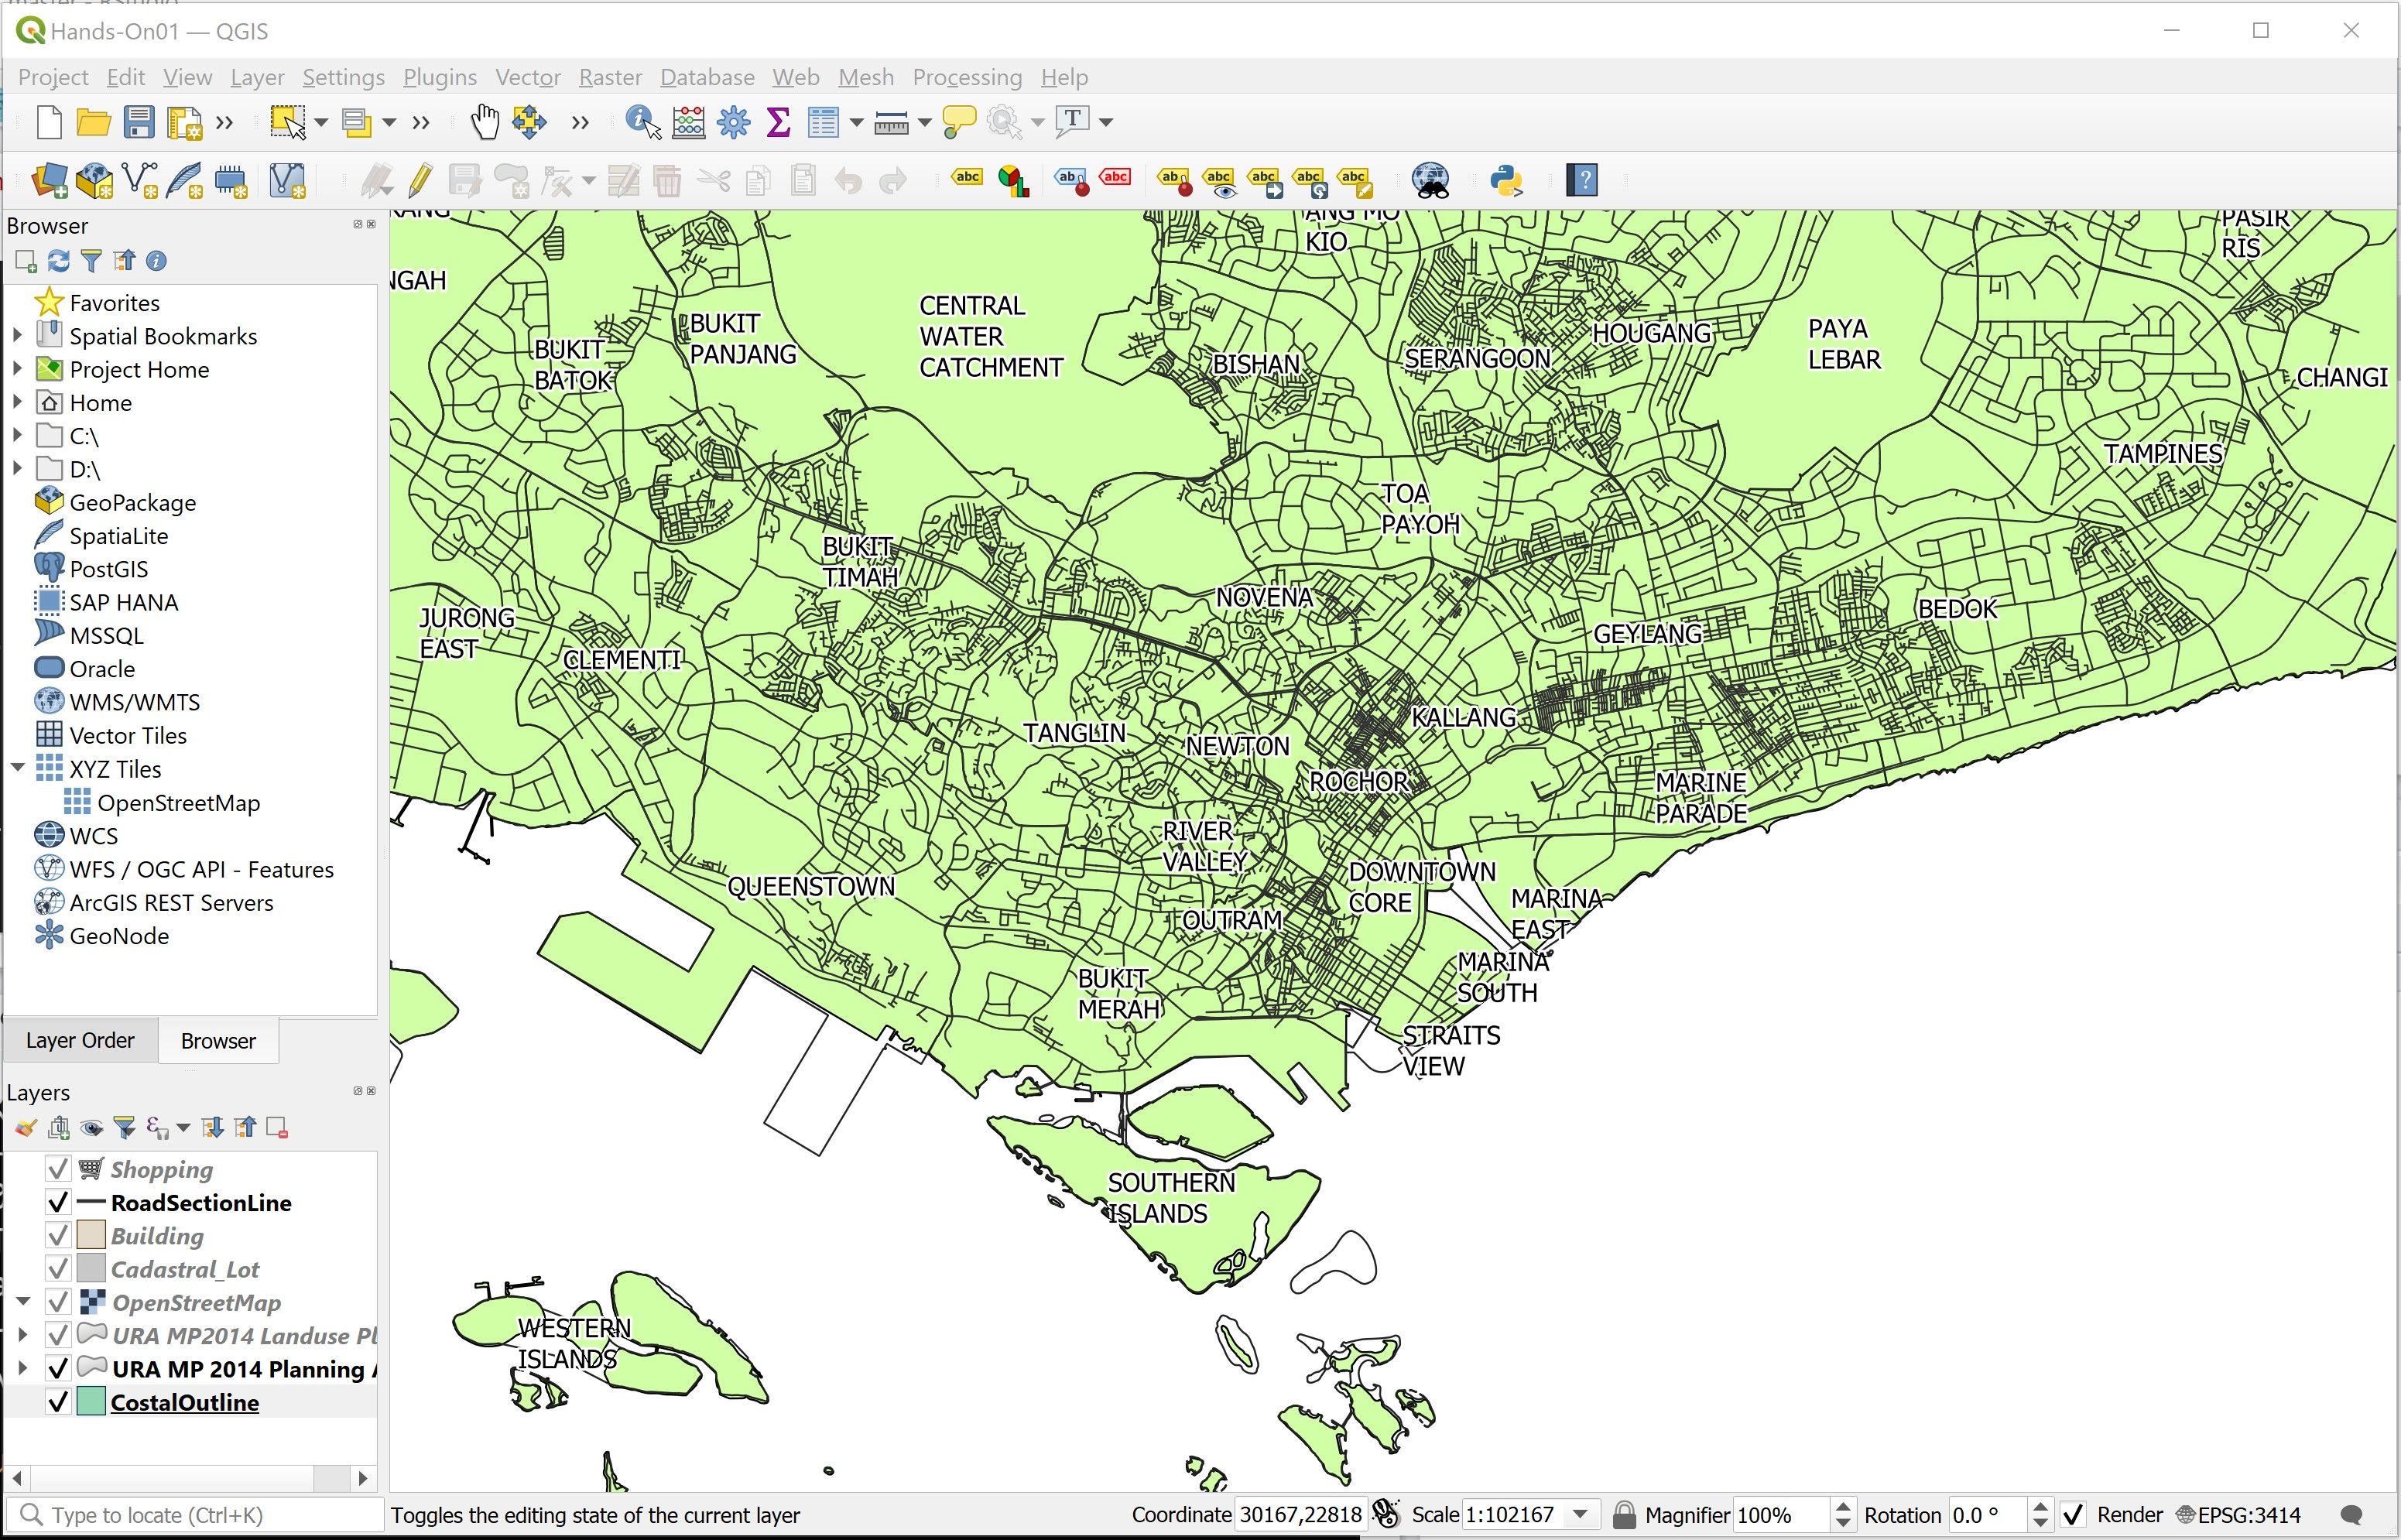
\includegraphics{./img/image1-14.jpg}

Notice that the map layer zooms into a new extent.

Now, you want to return to the previous extent.

\begin{itemize}
\tightlist
\item
  From \textbf{Map Navigation Toolbar}, click on the \textbf{Zoom Last}
  tool.
\end{itemize}

Notice that the map view returns to the initial extant now.

Next, you will learn how to zoom into a specific location using the Zoom
In tool. For example, we would like to zoom into the mark area as shown
in the figure below.

\begin{itemize}
\tightlist
\item
  From \textbf{Map Navigation Toolbar}, click on the \textbf{Zoom In}
  tool.
\item
  Hover the mouse over Punggol Planning Area.
\item
  Press on the left button of the mouse, drag to form a rectangle around
  Puggol Planning Area.
\item
  Release the left button.
\end{itemize}

Your screen should look similar to the figure below. Notice that the URA
MP2014 Landuse Plan layer appears now.

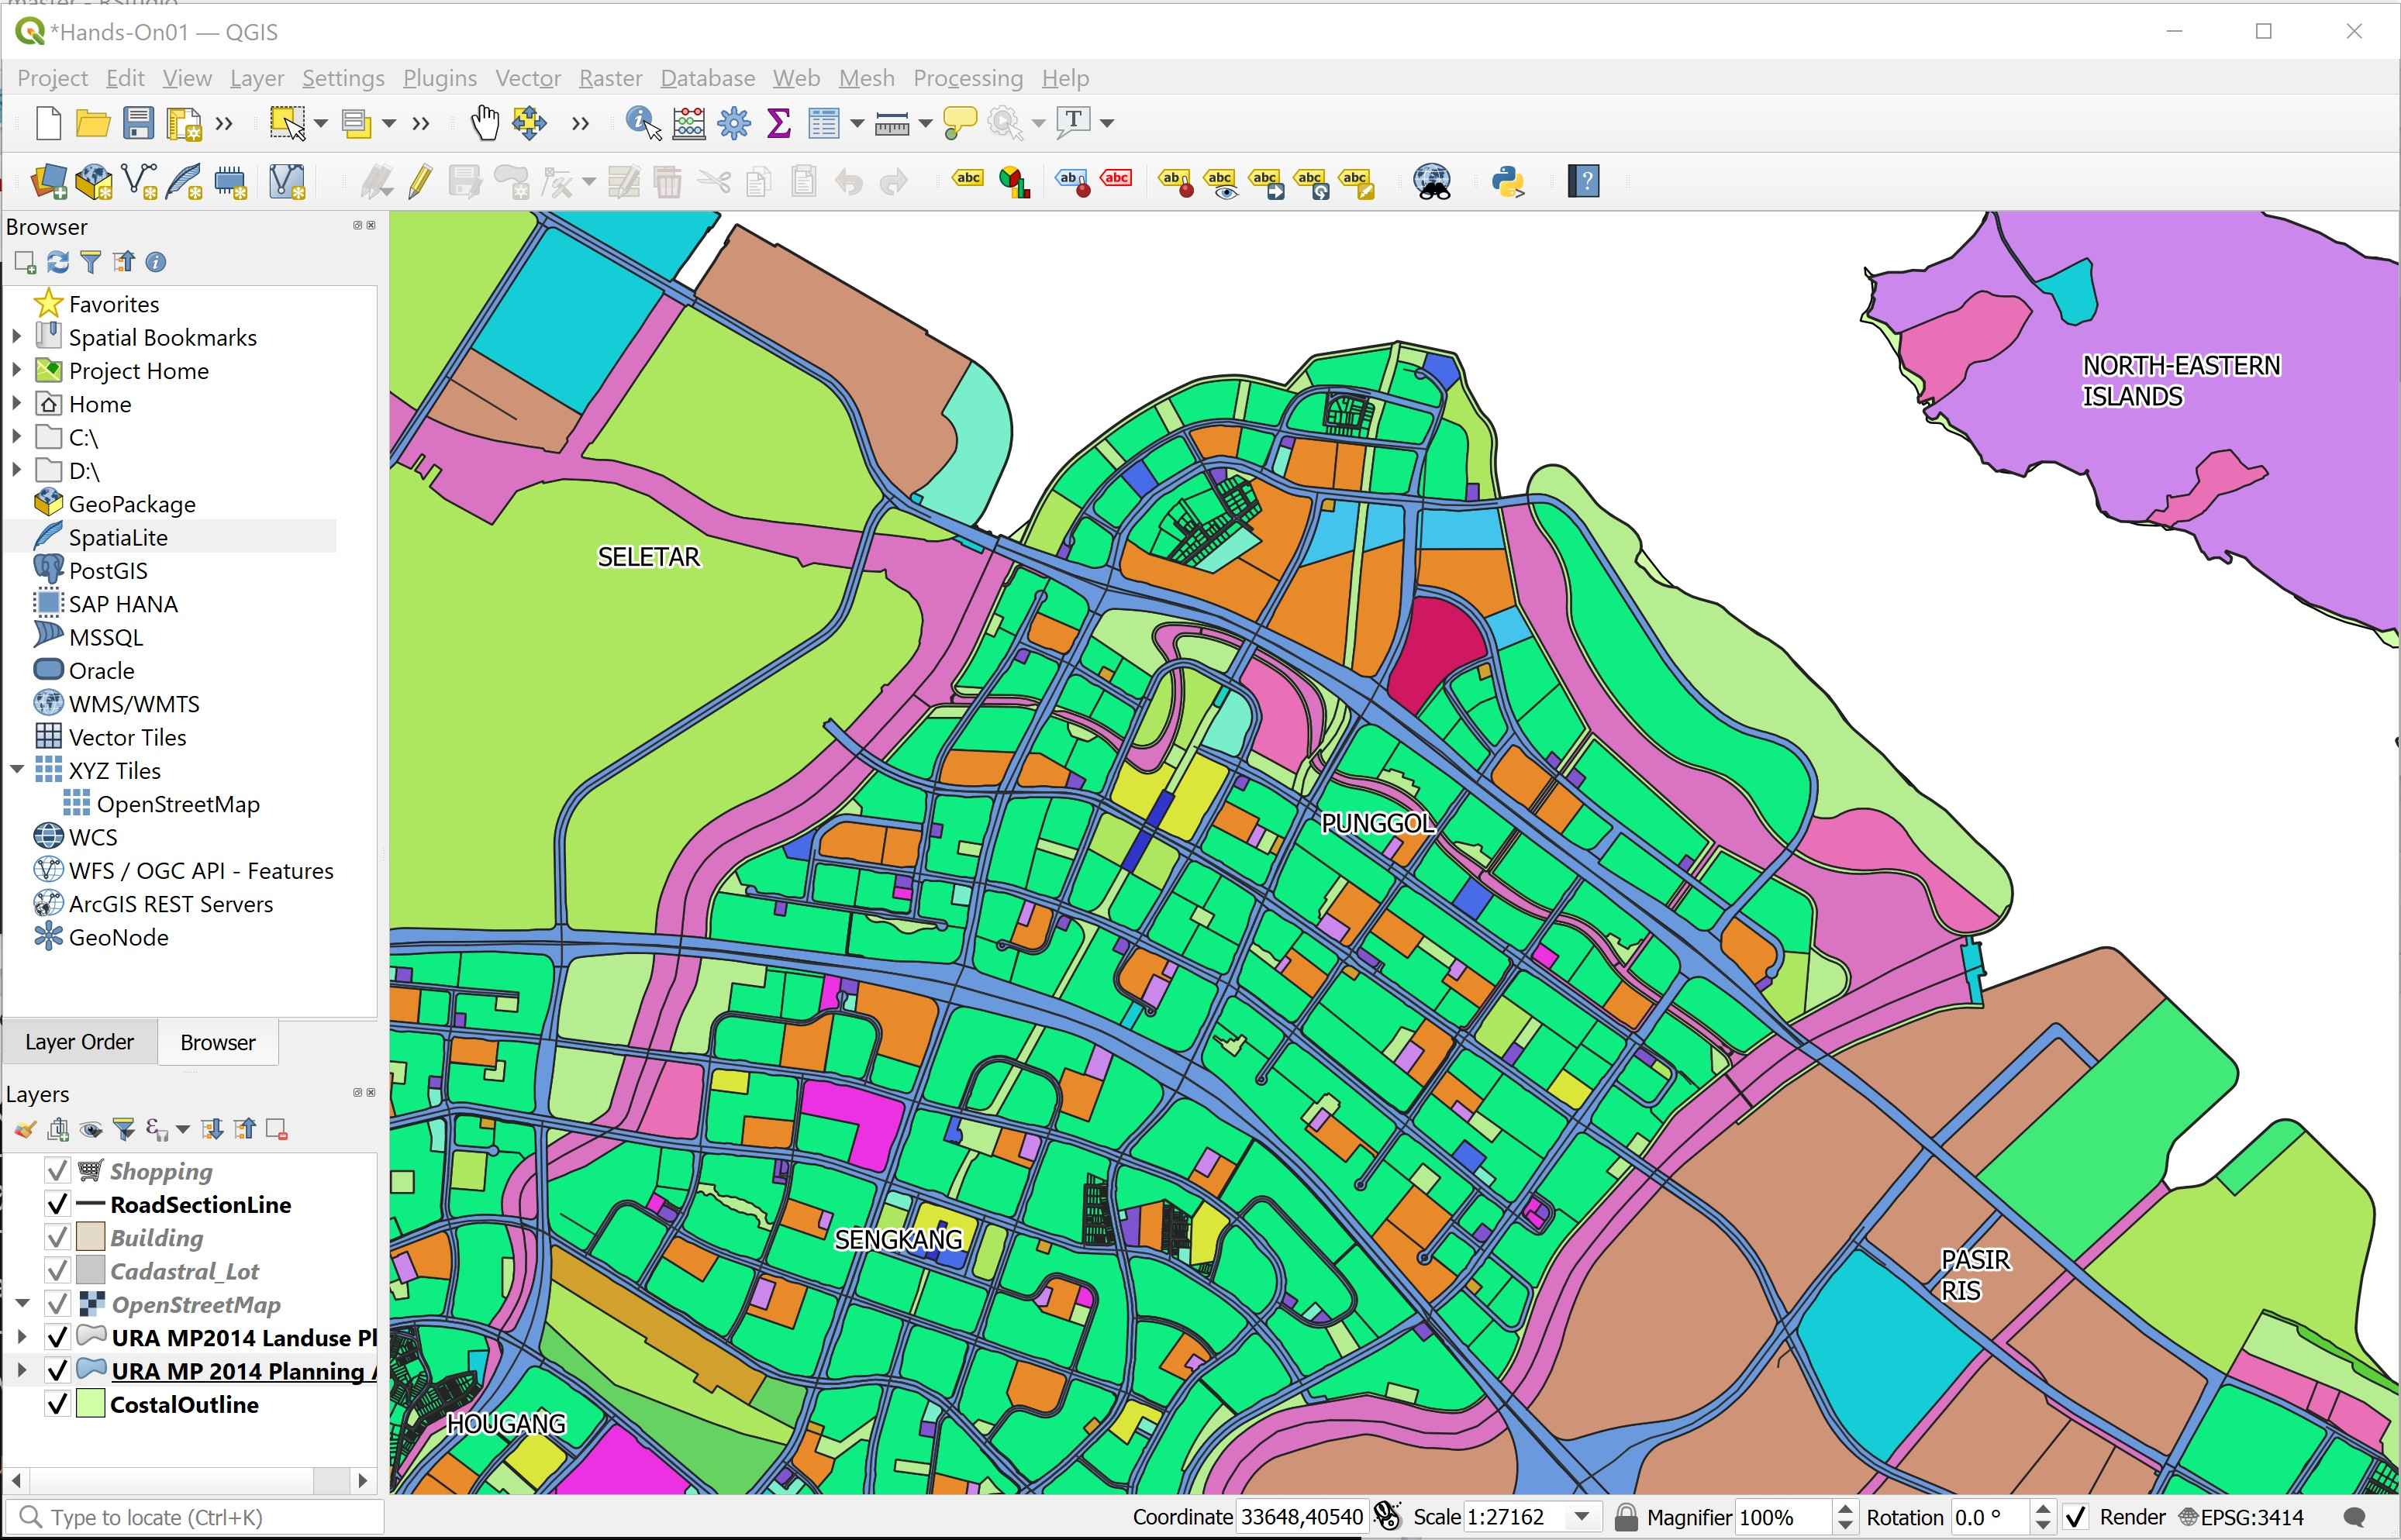
\includegraphics{./img/image1-15.jpg}

Next, you will return to the previous extent using alternative zooming
tool.

\begin{itemize}
\tightlist
\item
  From \textbf{Map Navigation Toolbar}, click on the \textbf{Zoom to
  Layer} tool.
\end{itemize}

Notice that the map view returns to the previous state and \emph{URA
MP2014 Landuse Plan} layers are turned off again.

\begin{quote}
DIY: Try out the remaining navigation tools in \textbf{Map Navigation
Toolbar}.
\end{quote}

\hypertarget{map-navigation-by-changing-the-map-scale}{%
\subsection{Map Navigation by changing the map
scale}\label{map-navigation-by-changing-the-map-scale}}

In this section, you will learn how to change the map view by changing
the map scale.

\begin{itemize}
\tightlist
\item
  From the \textbf{Status bar} (located below Map View), click on the
  drop-down list of \textbf{Scale}.
\item
  Select \textbf{1:25,000}.
\item
  Use the \textbf{Pan tool} to move the map area so that it looks
  similar to the figure below.
\end{itemize}

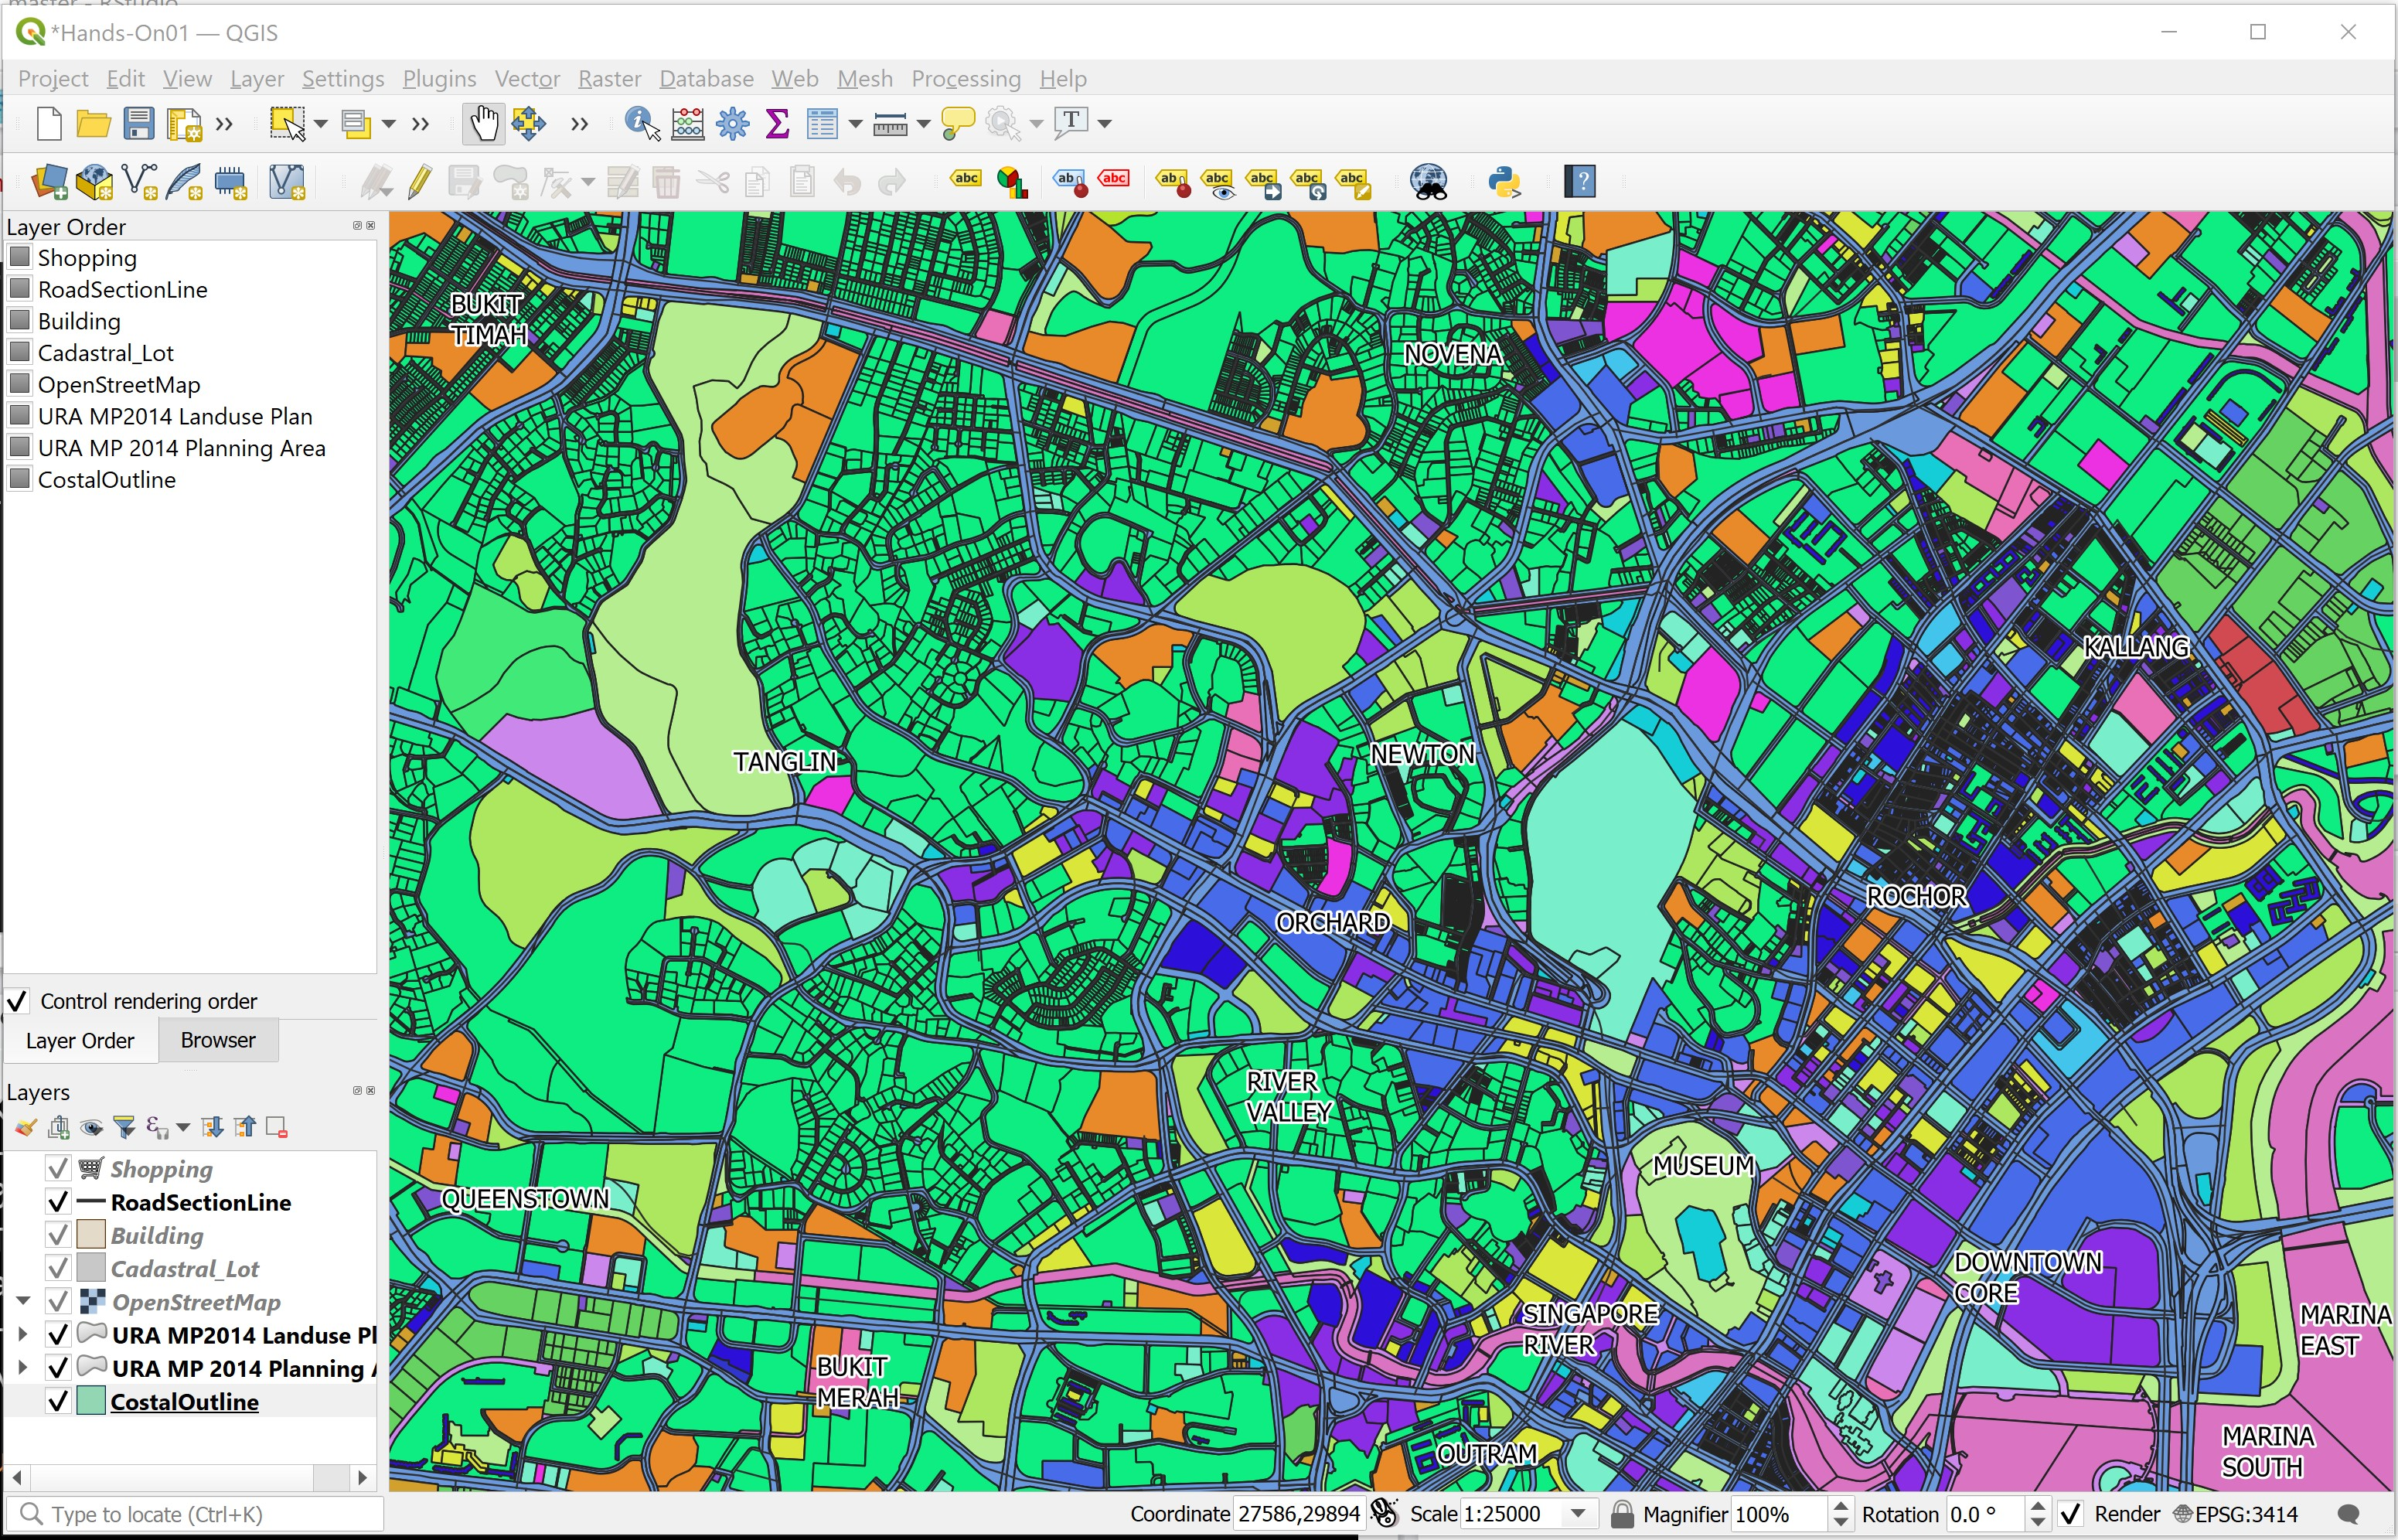
\includegraphics{./img/image1-16.jpg}

\begin{itemize}
\tightlist
\item
  From the \textbf{Scale} of at the \textbf{Status bar}, click on the
  drop-down list again.
\item
  Select \textbf{1:4500}.
\end{itemize}

Your screen should look similar to the figure below. Notice that more
detail appears when the map scale increases.

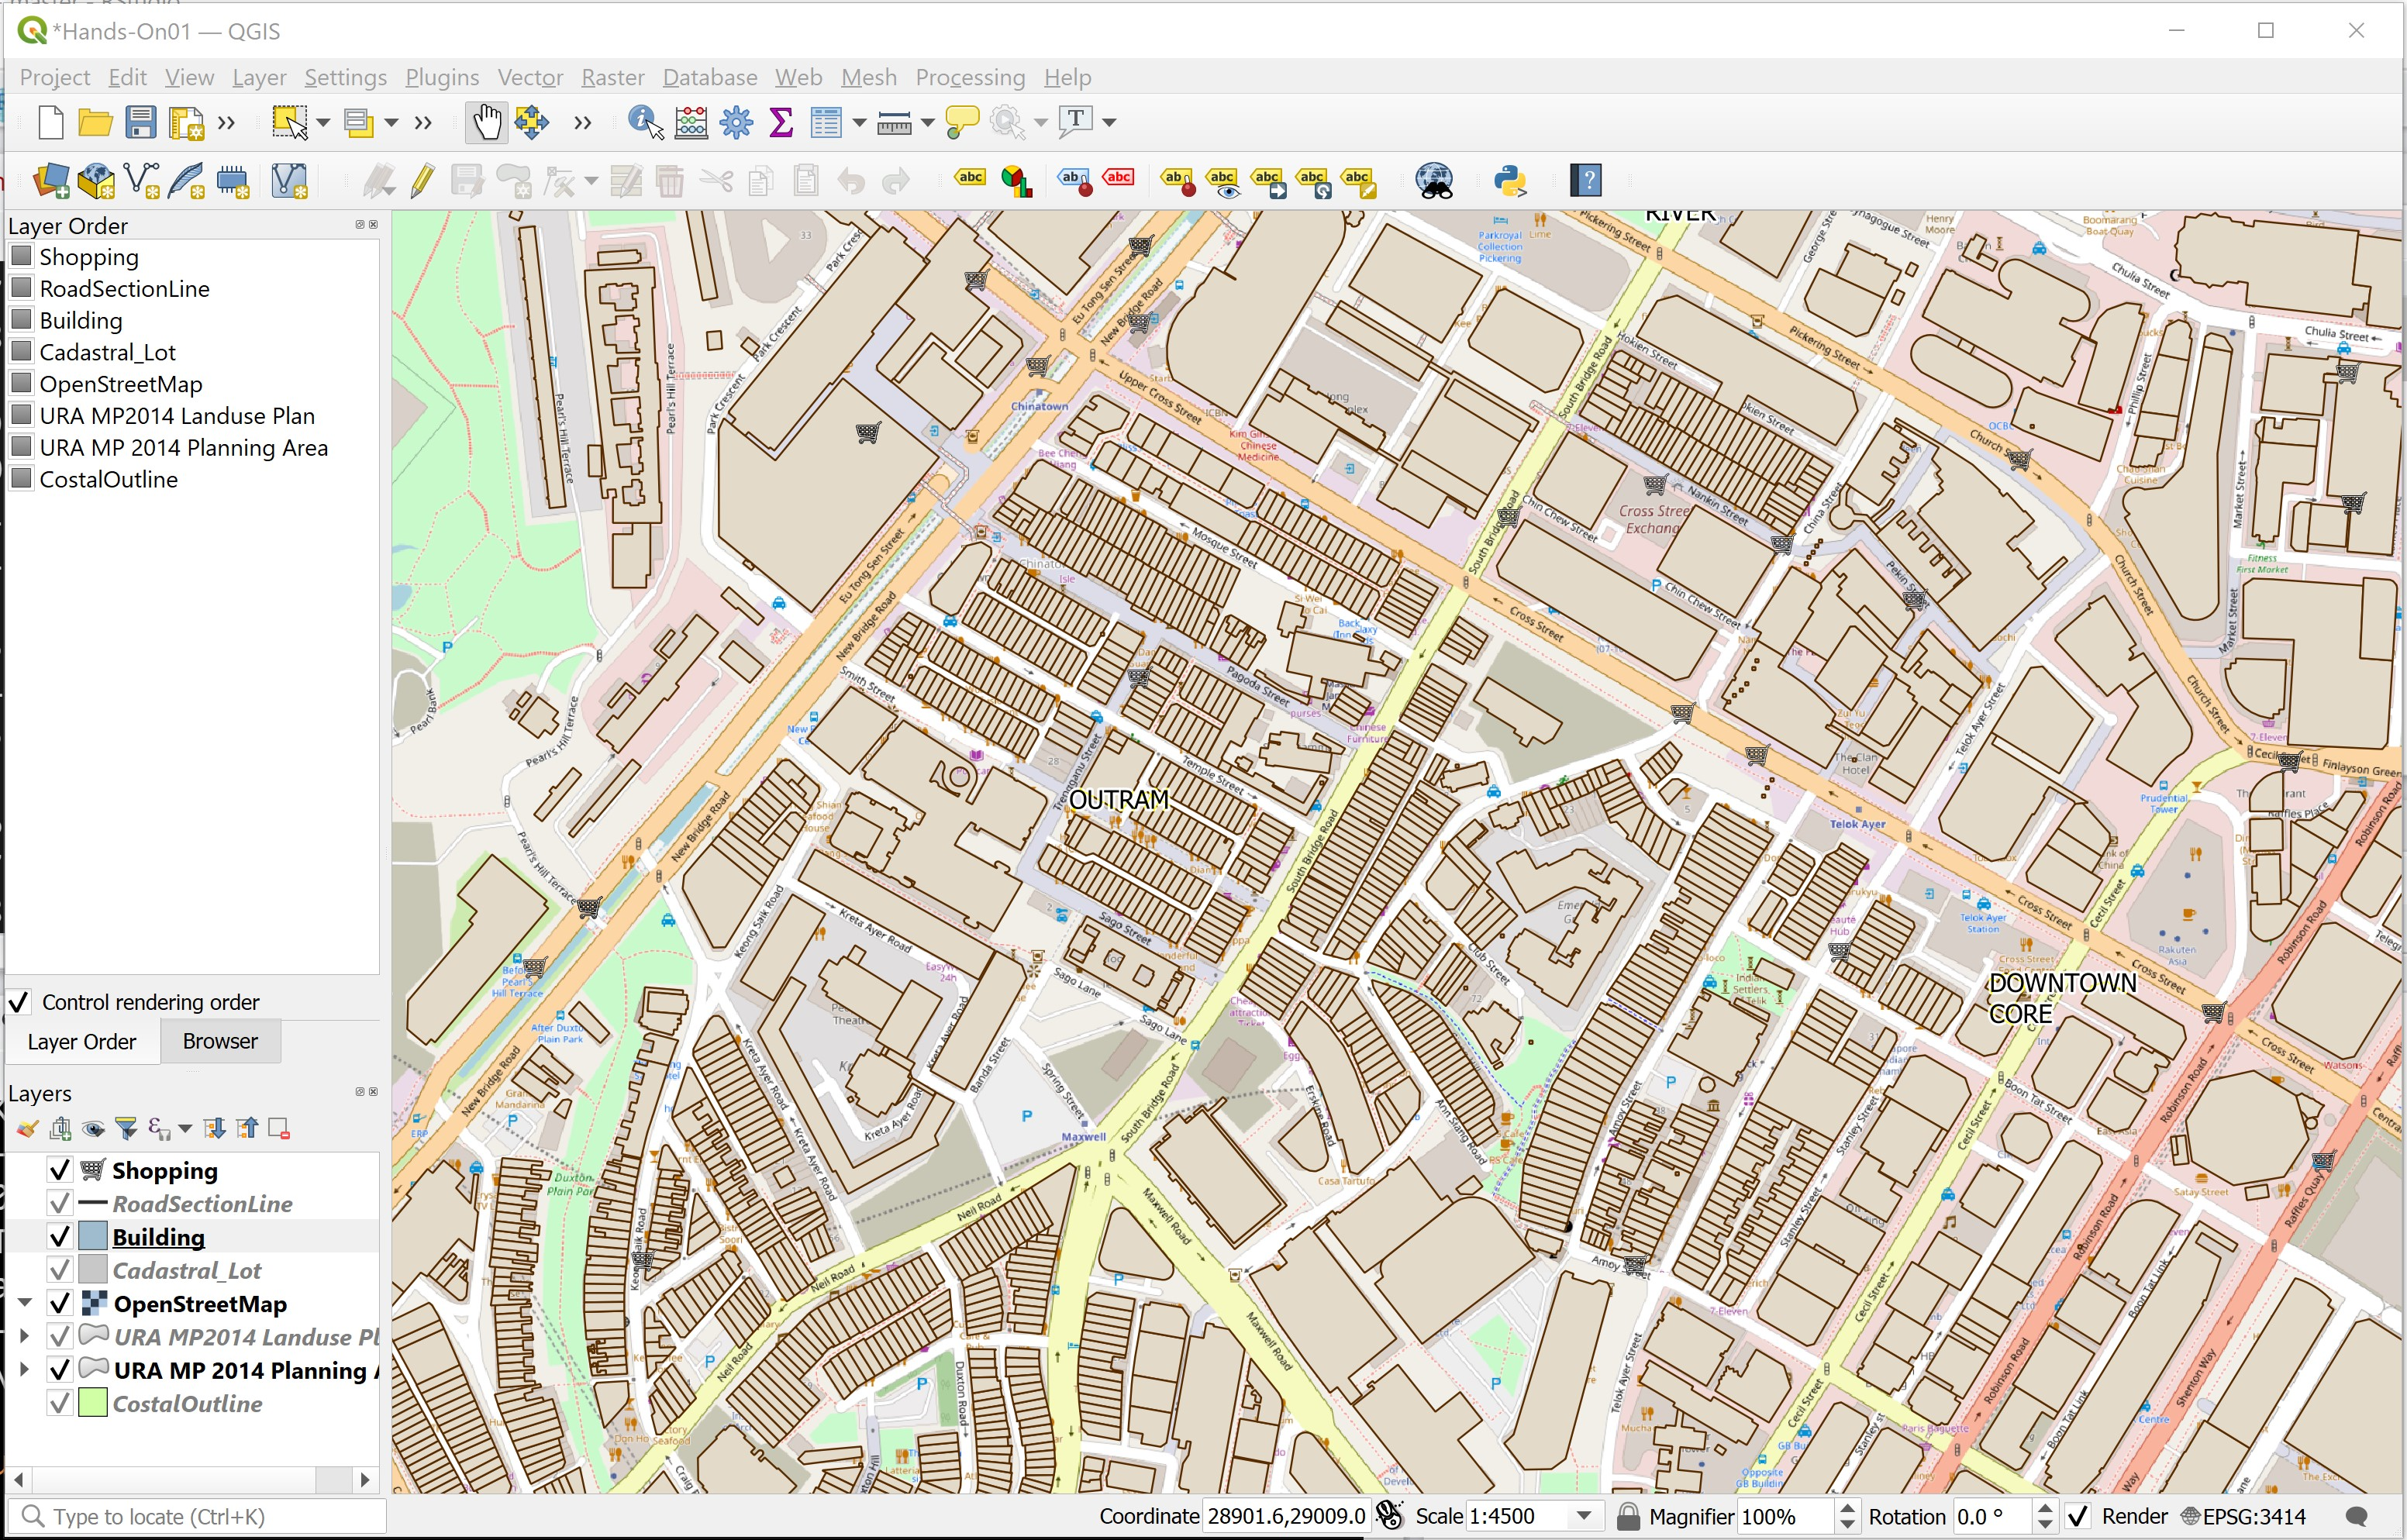
\includegraphics{./img/image1-17.jpg}

\hypertarget{exploring-gis-data}{%
\section{Exploring GIS data}\label{exploring-gis-data}}

In this section, you will learn how to interact with the features that
appear in the Map View and retrieve their corresponding attribute
information.

\hypertarget{exploring-gis-layer}{%
\subsection{Exploring GIS Layer}\label{exploring-gis-layer}}

In this sub-section, you will learn how to explore the information of
individual GIS layer.

\begin{itemize}
\tightlist
\item
  From the \textbf{Map Legend} window, right-click on \texttt{Building}
  layer.
\item
  Select \textbf{Properties} from the context menu.
\end{itemize}

The Layer Properties of Building layer appears. It provides the full
metadata of Building layer, it symbolization configuration and the data
fields.

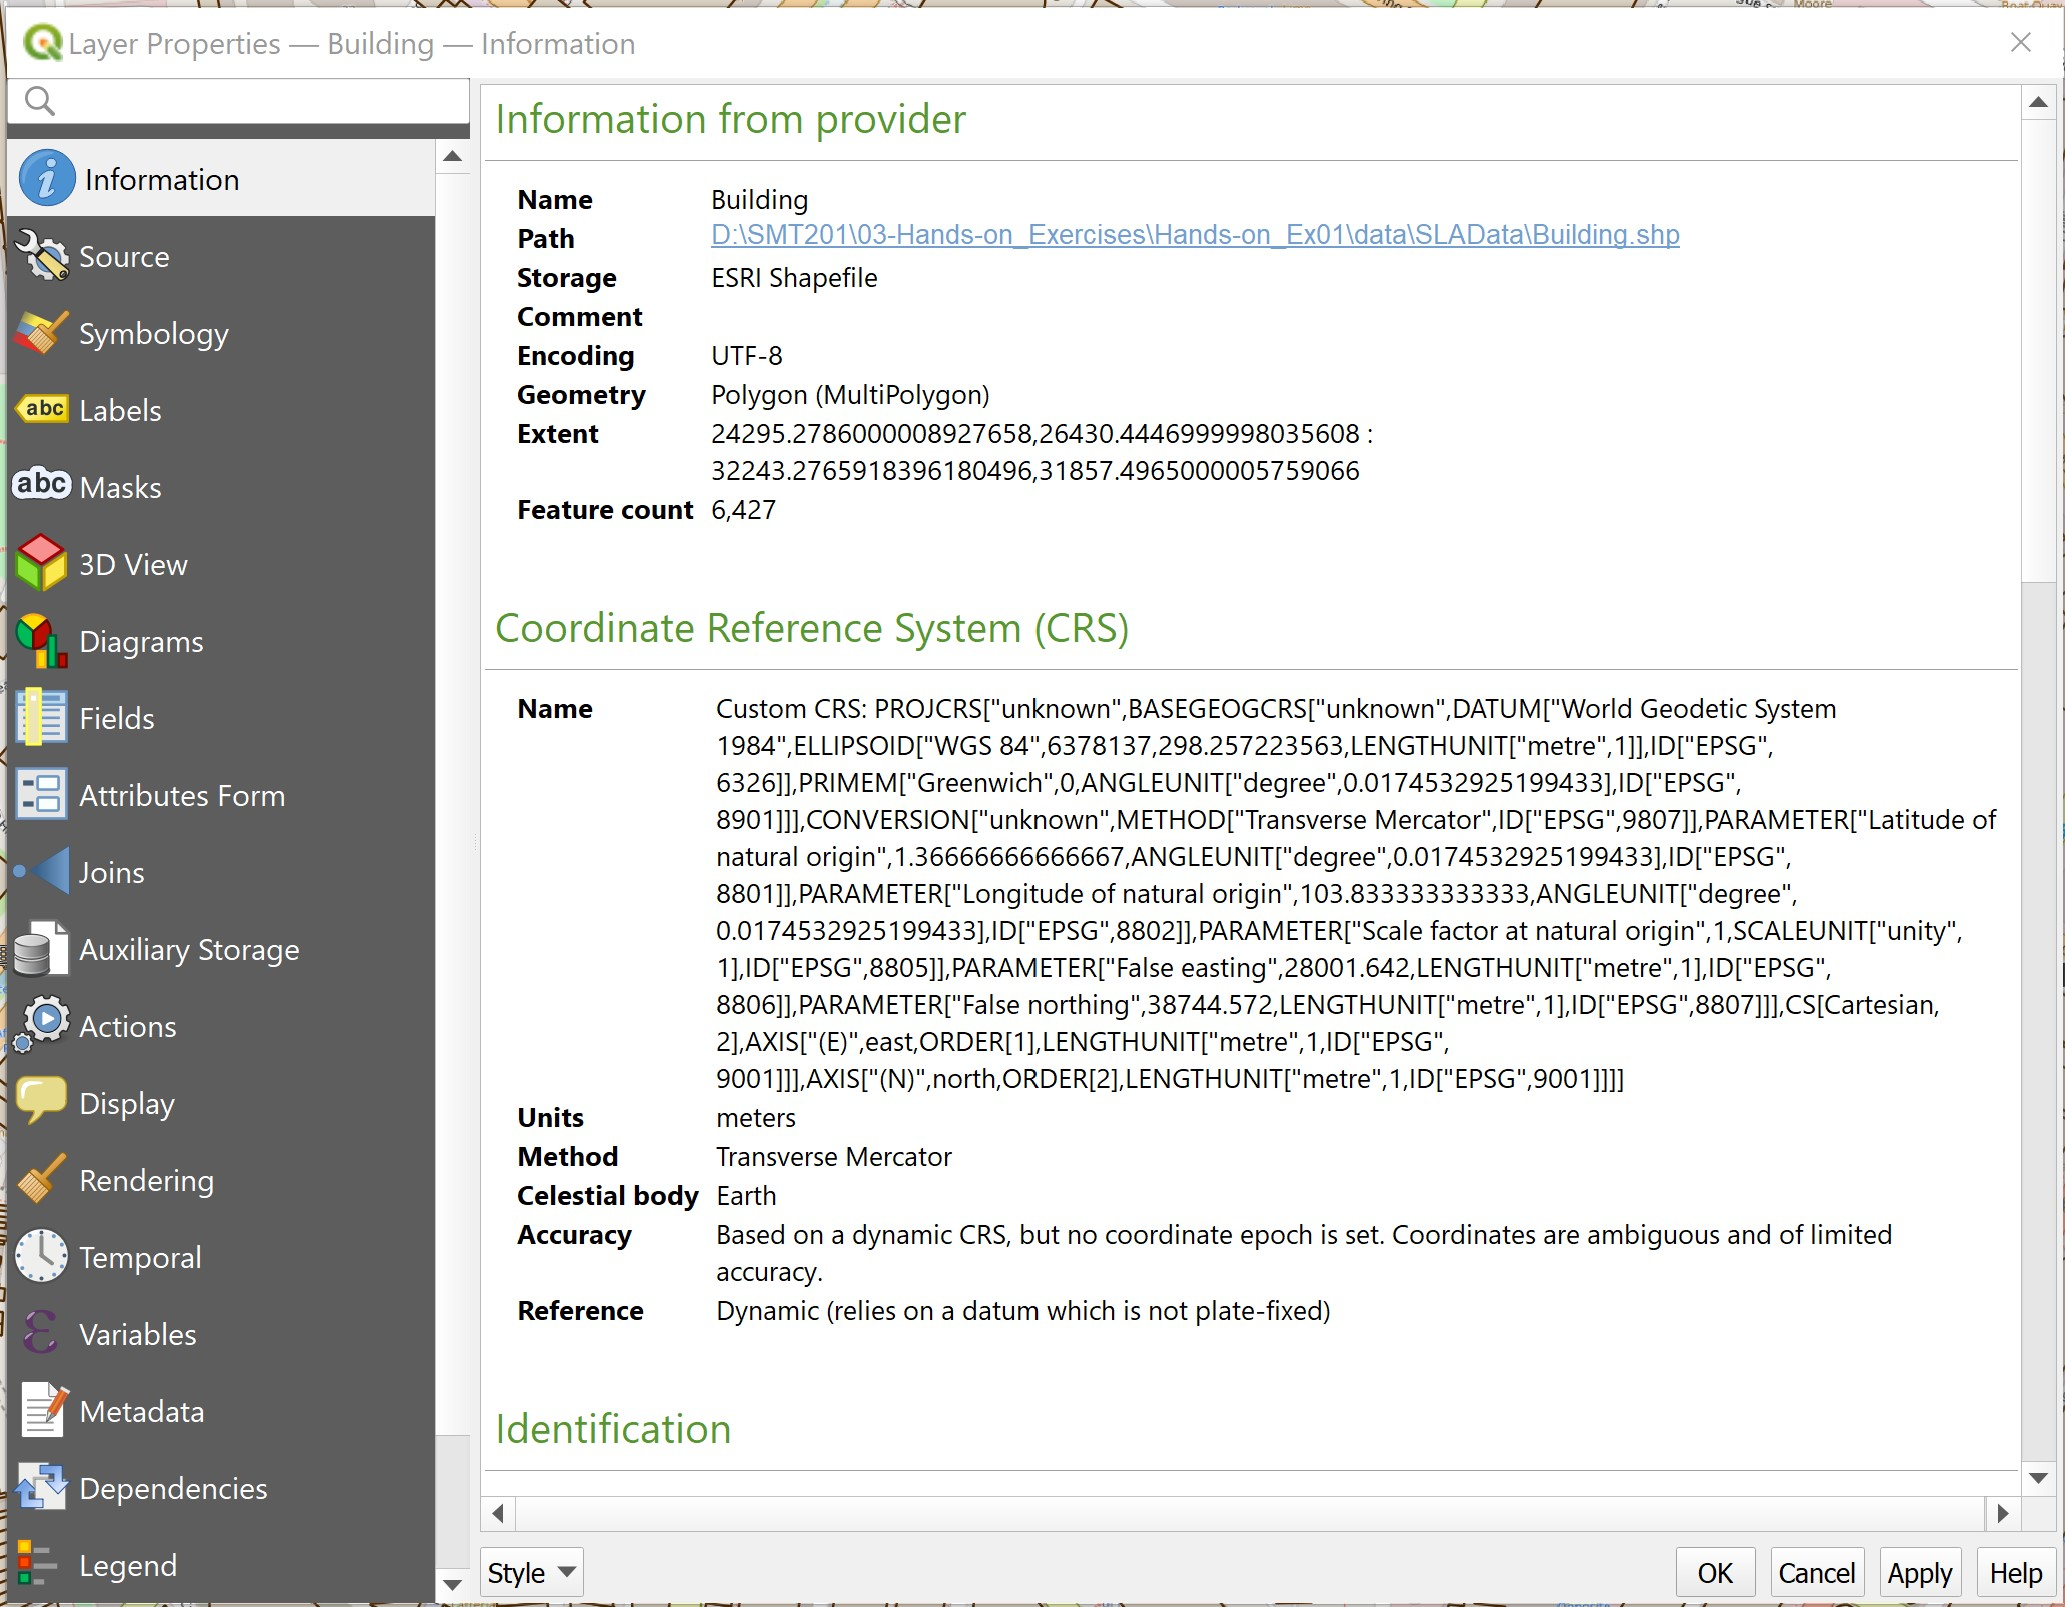
\includegraphics{./img/image1-18.jpg}

By default, QGIS will display the general information of the selected
layer. You can retrieve other information or configurations of the layer
by clicking on the appropriate tab.

The key information available are as follows:

\begin{itemize}
\tightlist
\item
  Source shows the path of Building layer.
\item
  Storage reveals the file type, i.e.~ESRI Shapefile format.
\item
  Geometry indicate the spatial object used to represent the real world
  feature.\\
\item
  CRS shows the georeferencing information of the active layer
  (i.e.~SVY21/Singapore TM).
\item
  Unit is the unit measurement of the active layer.
\end{itemize}

Let us examine other tab.

• Click on \textbf{Rendering} tab.

You screen should look similar to the figure below.

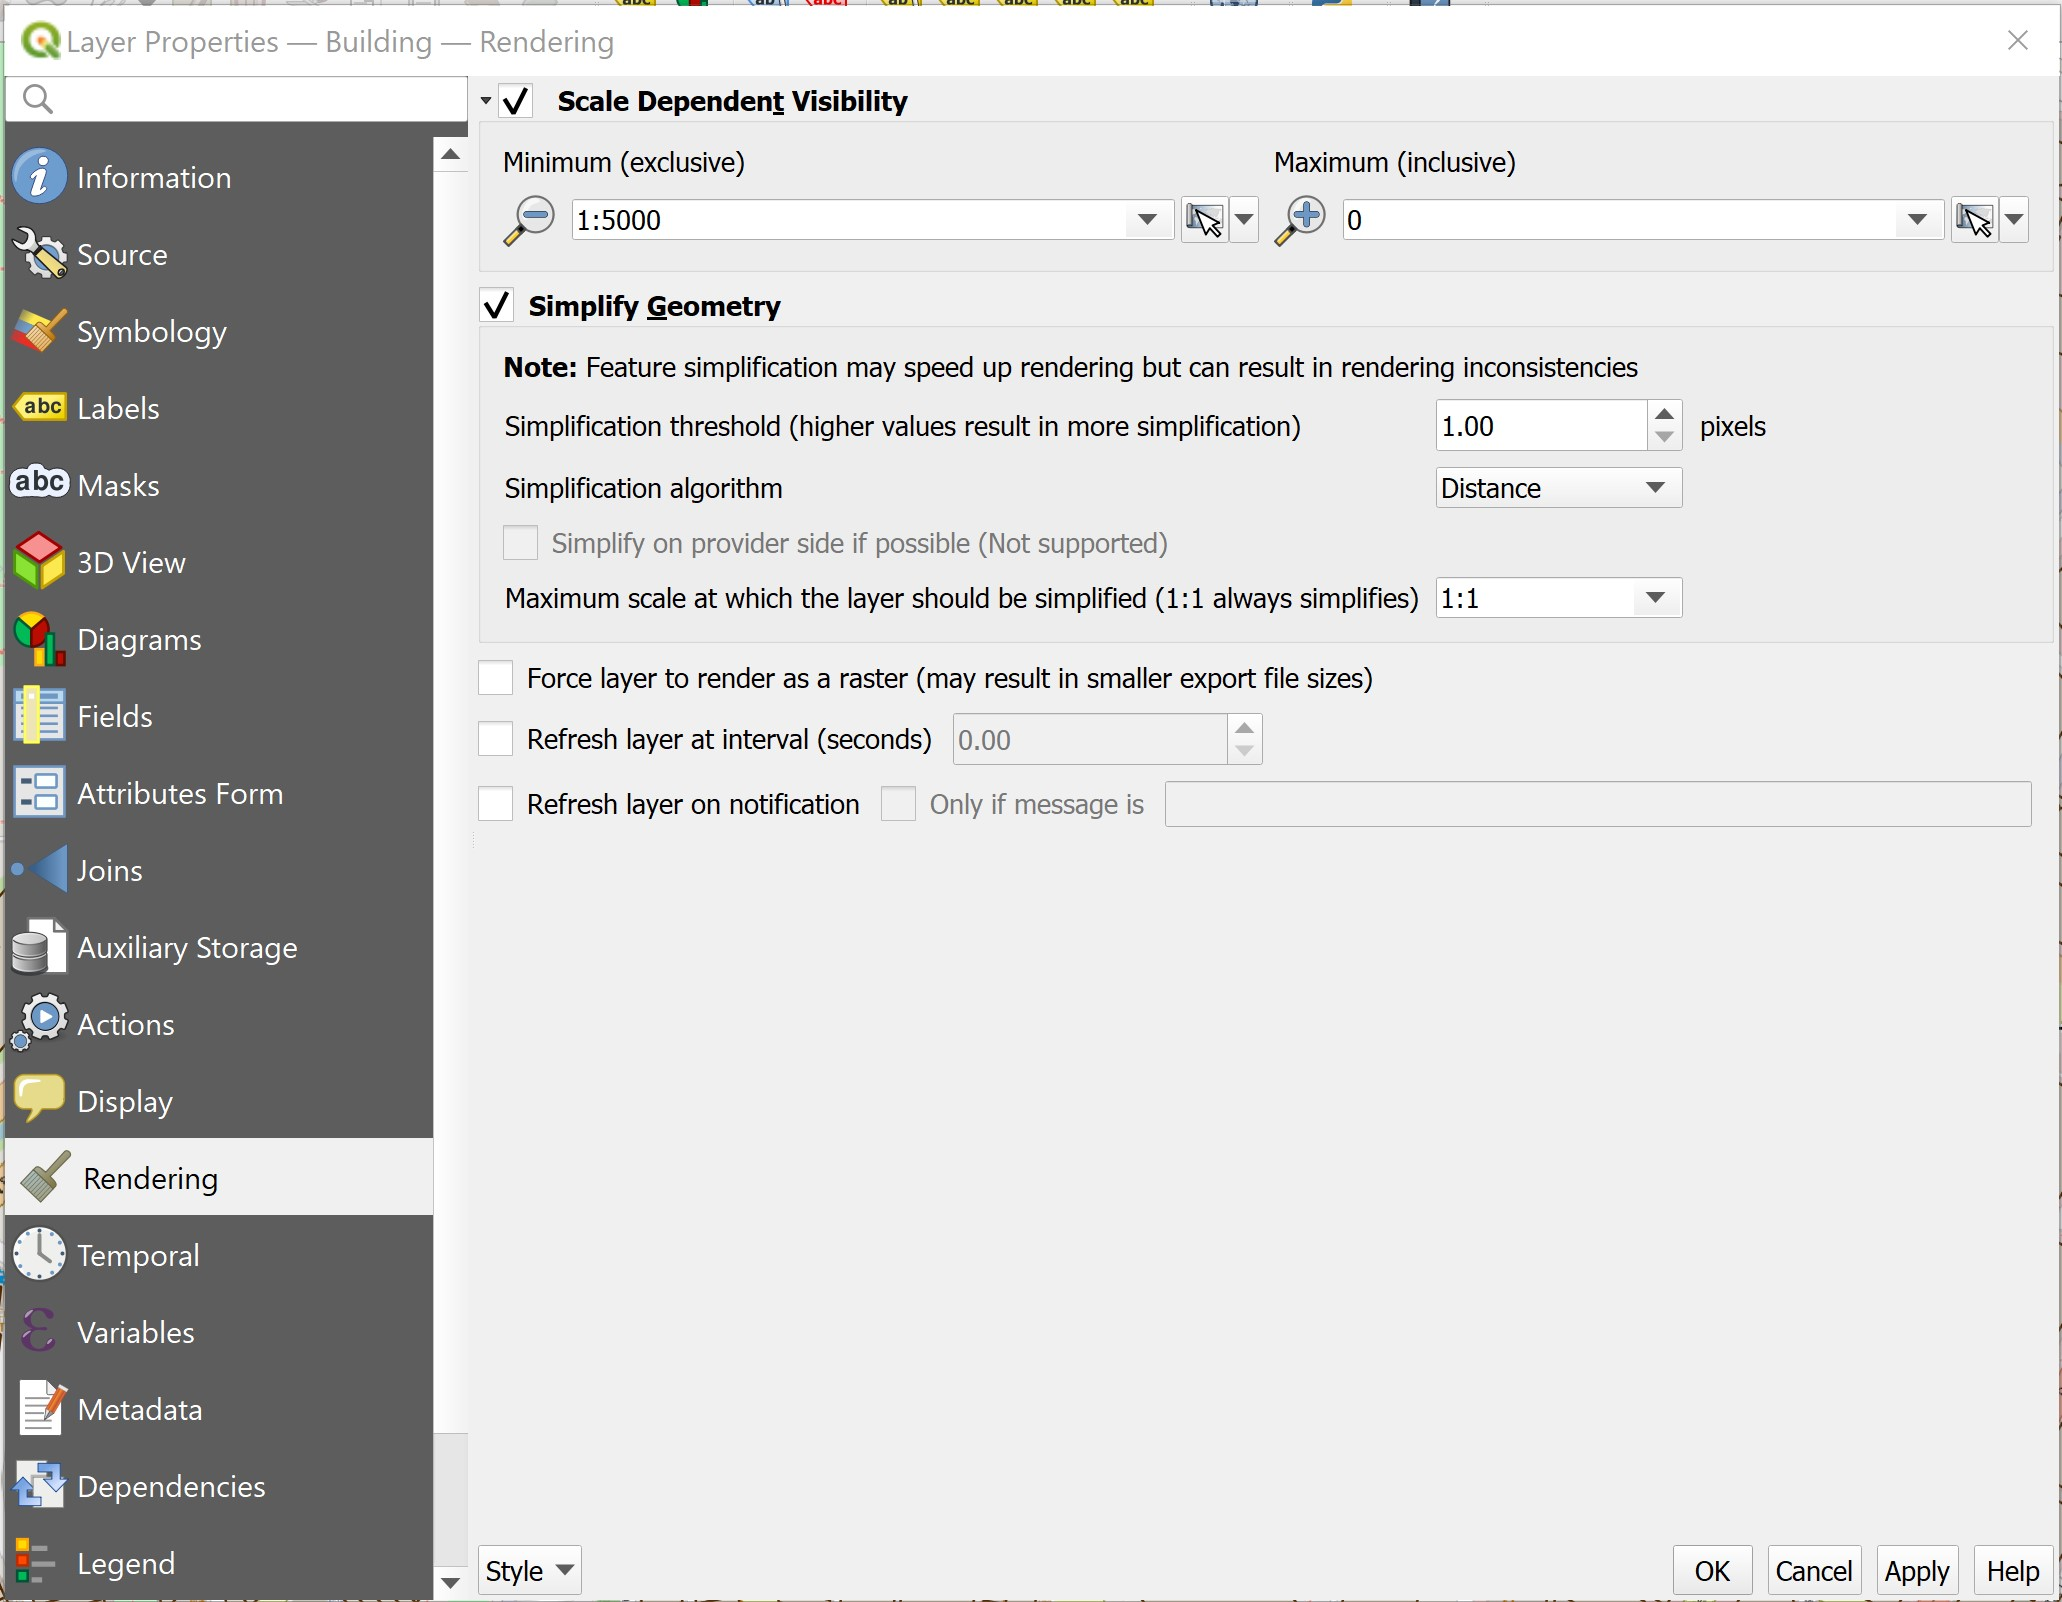
\includegraphics{./img/image1-19.jpg}

Note that and the minimum map scale is 5000. That explains why the
building layer only appears when the map scale of Map View is less than
or equal to 1:5000.

Next, you will explore the data fields of Building layer.

\begin{itemize}
\tightlist
\item
  Click on the \textbf{Field} tab.
\end{itemize}

Your screen should look similar to the figure below.

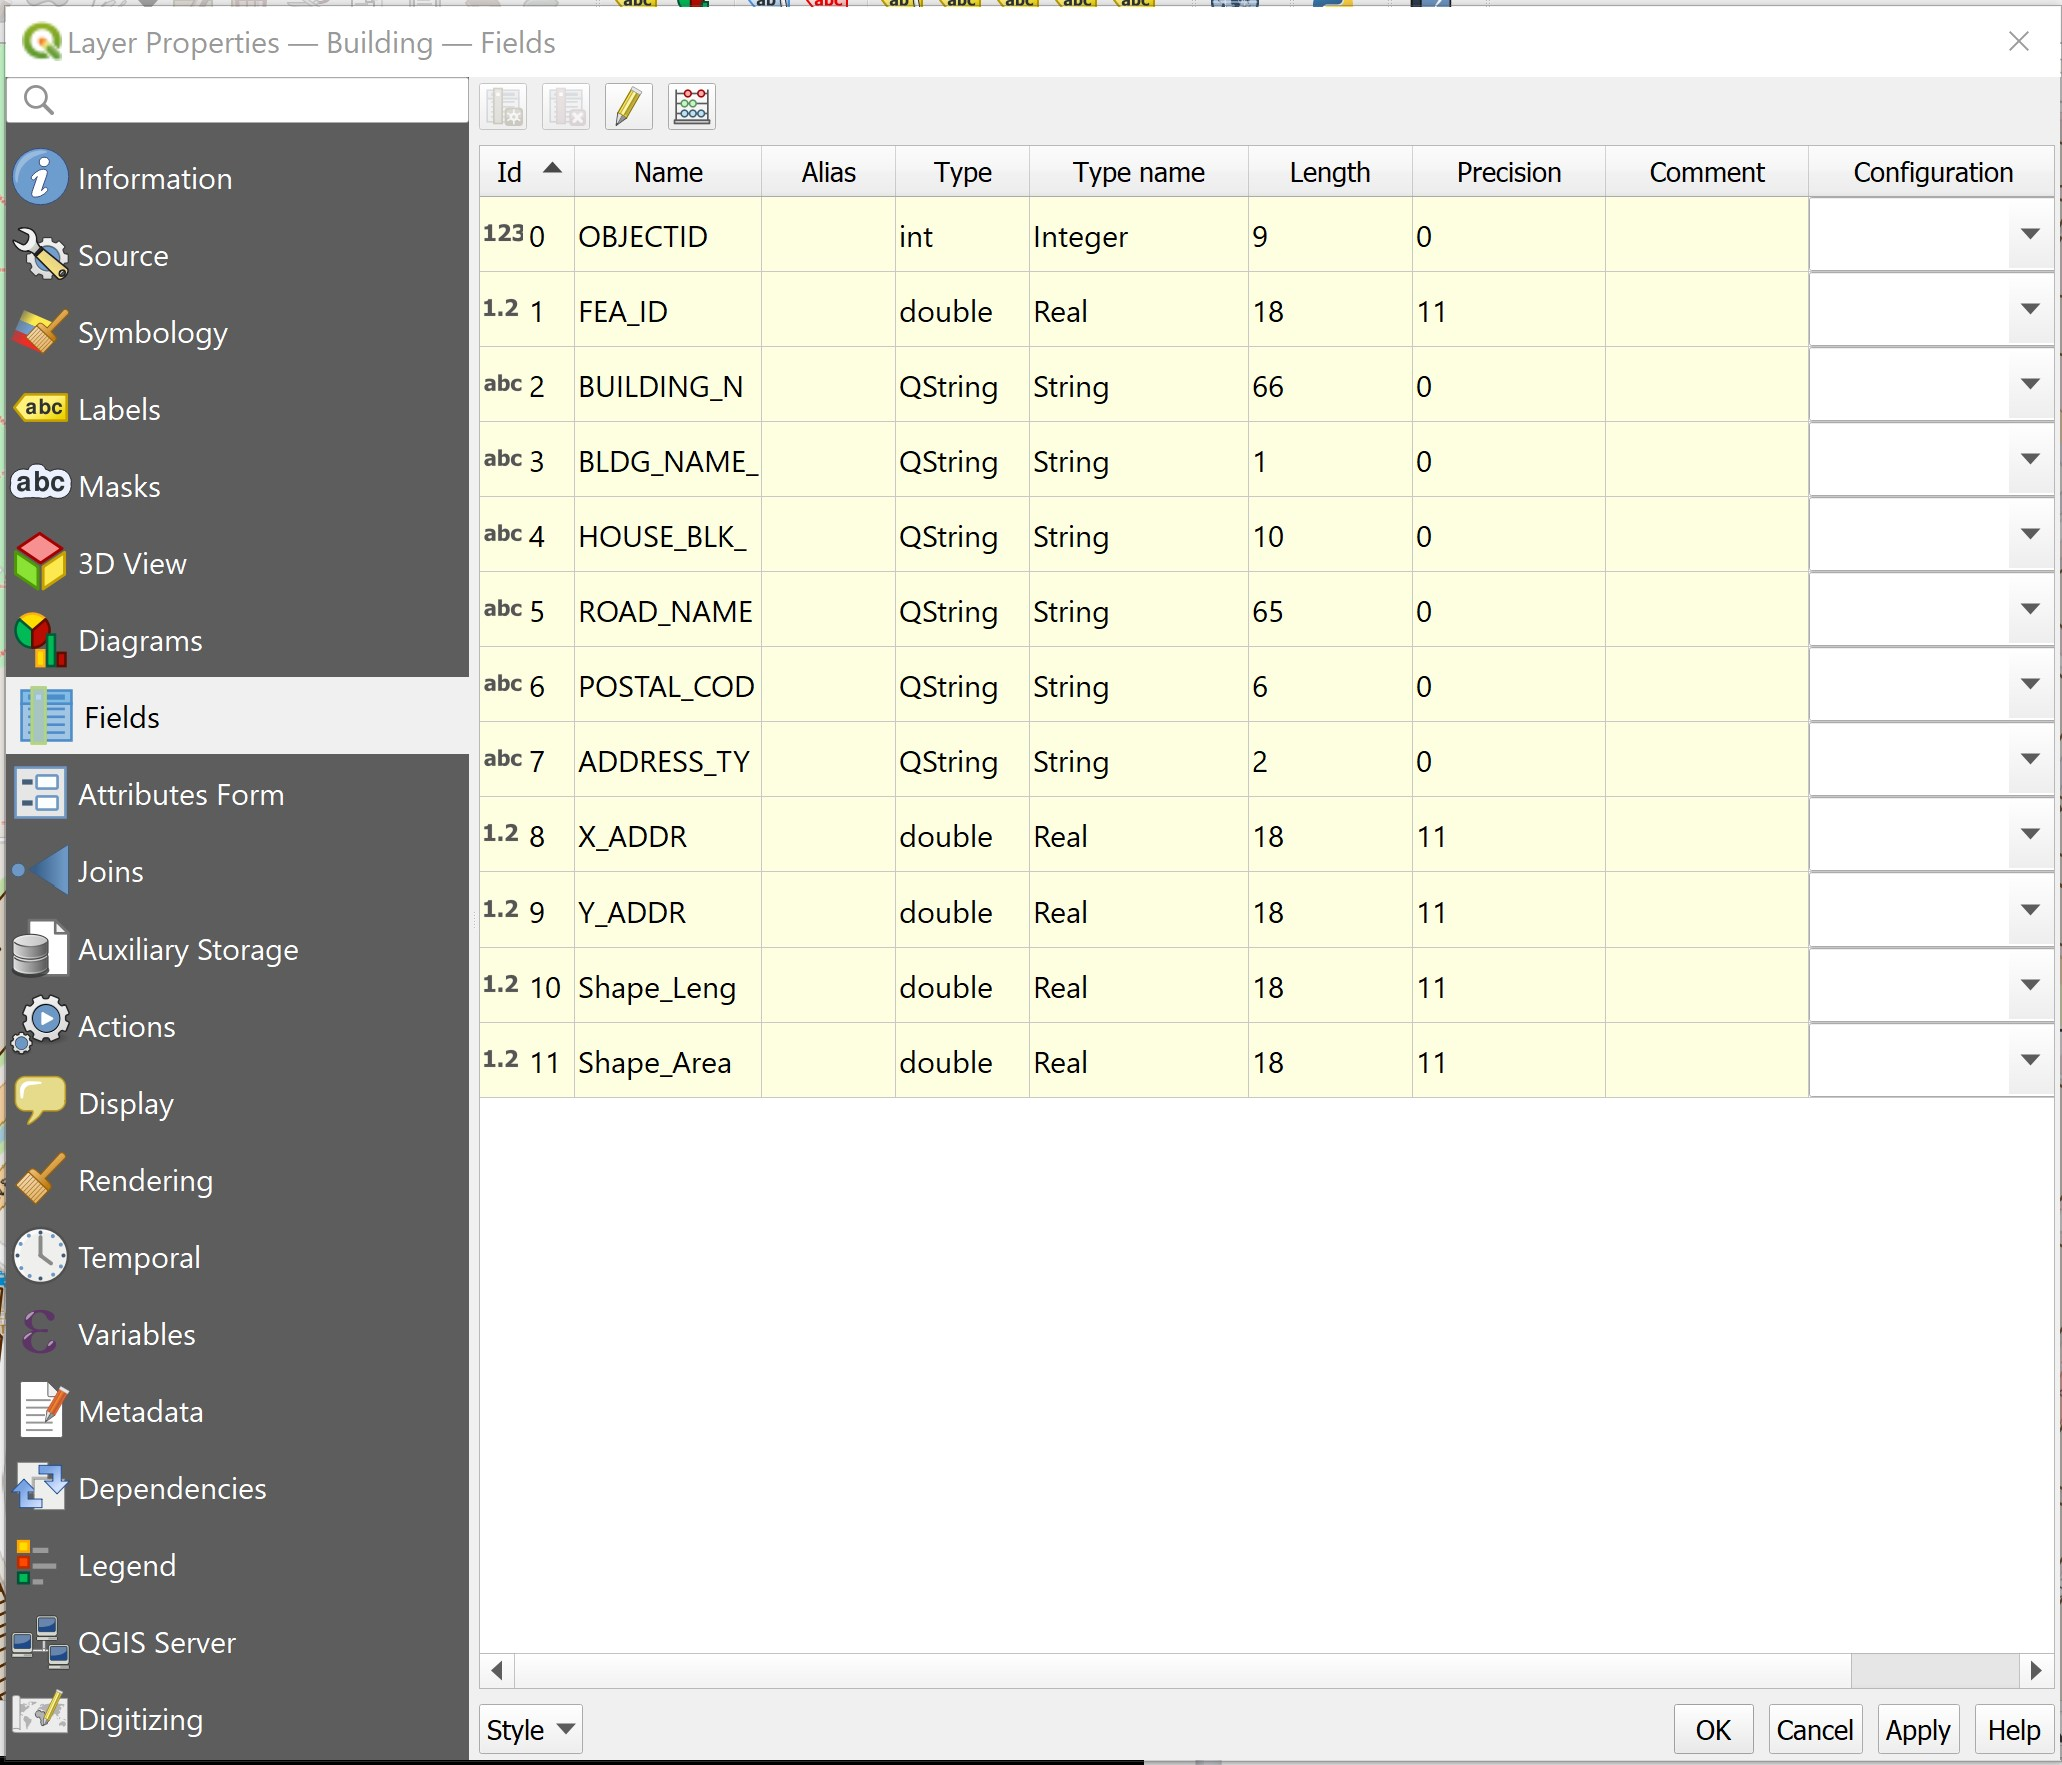
\includegraphics{./img/image1-20.jpg}

Notice that there are 12 fields in the corresponding attribute table of
Building layer. The Layer Properties window also shows the data type,
length and precision of each field.

You will explore the other tabs in the next hands-on.

\begin{itemize}
\tightlist
\item
  At the \textbf{Layer Properties} window, click on the cross button
  located at the upper right hand corner to close the window.
\end{itemize}

\hypertarget{working-with-identify-features-tool}{%
\subsection{Working with Identify Features
tool}\label{working-with-identify-features-tool}}

Using \textbf{Identify Features} tool to interact with a geographical
feature and retrieve its corresponding attribute information is a two
steps process. First, you need to make the layer of the feature active.
Then, you will use the Identify Features tool to query the information.

In this section, you will learn how to query information of a selected
Shopping feature (marks by a circle in the figure above).

• At the \textbf{Map Legend} window, click on \texttt{Shopping} layer to
make it active.

• Click on the \textbf{Identify Features} tool.

• At the \textbf{Map View} window, hovers the mouse over the shopping
feature you are interested to query (the one marked in the figure
above).

• Click on an shopping feature.

Your screen should look similar to the figure below.

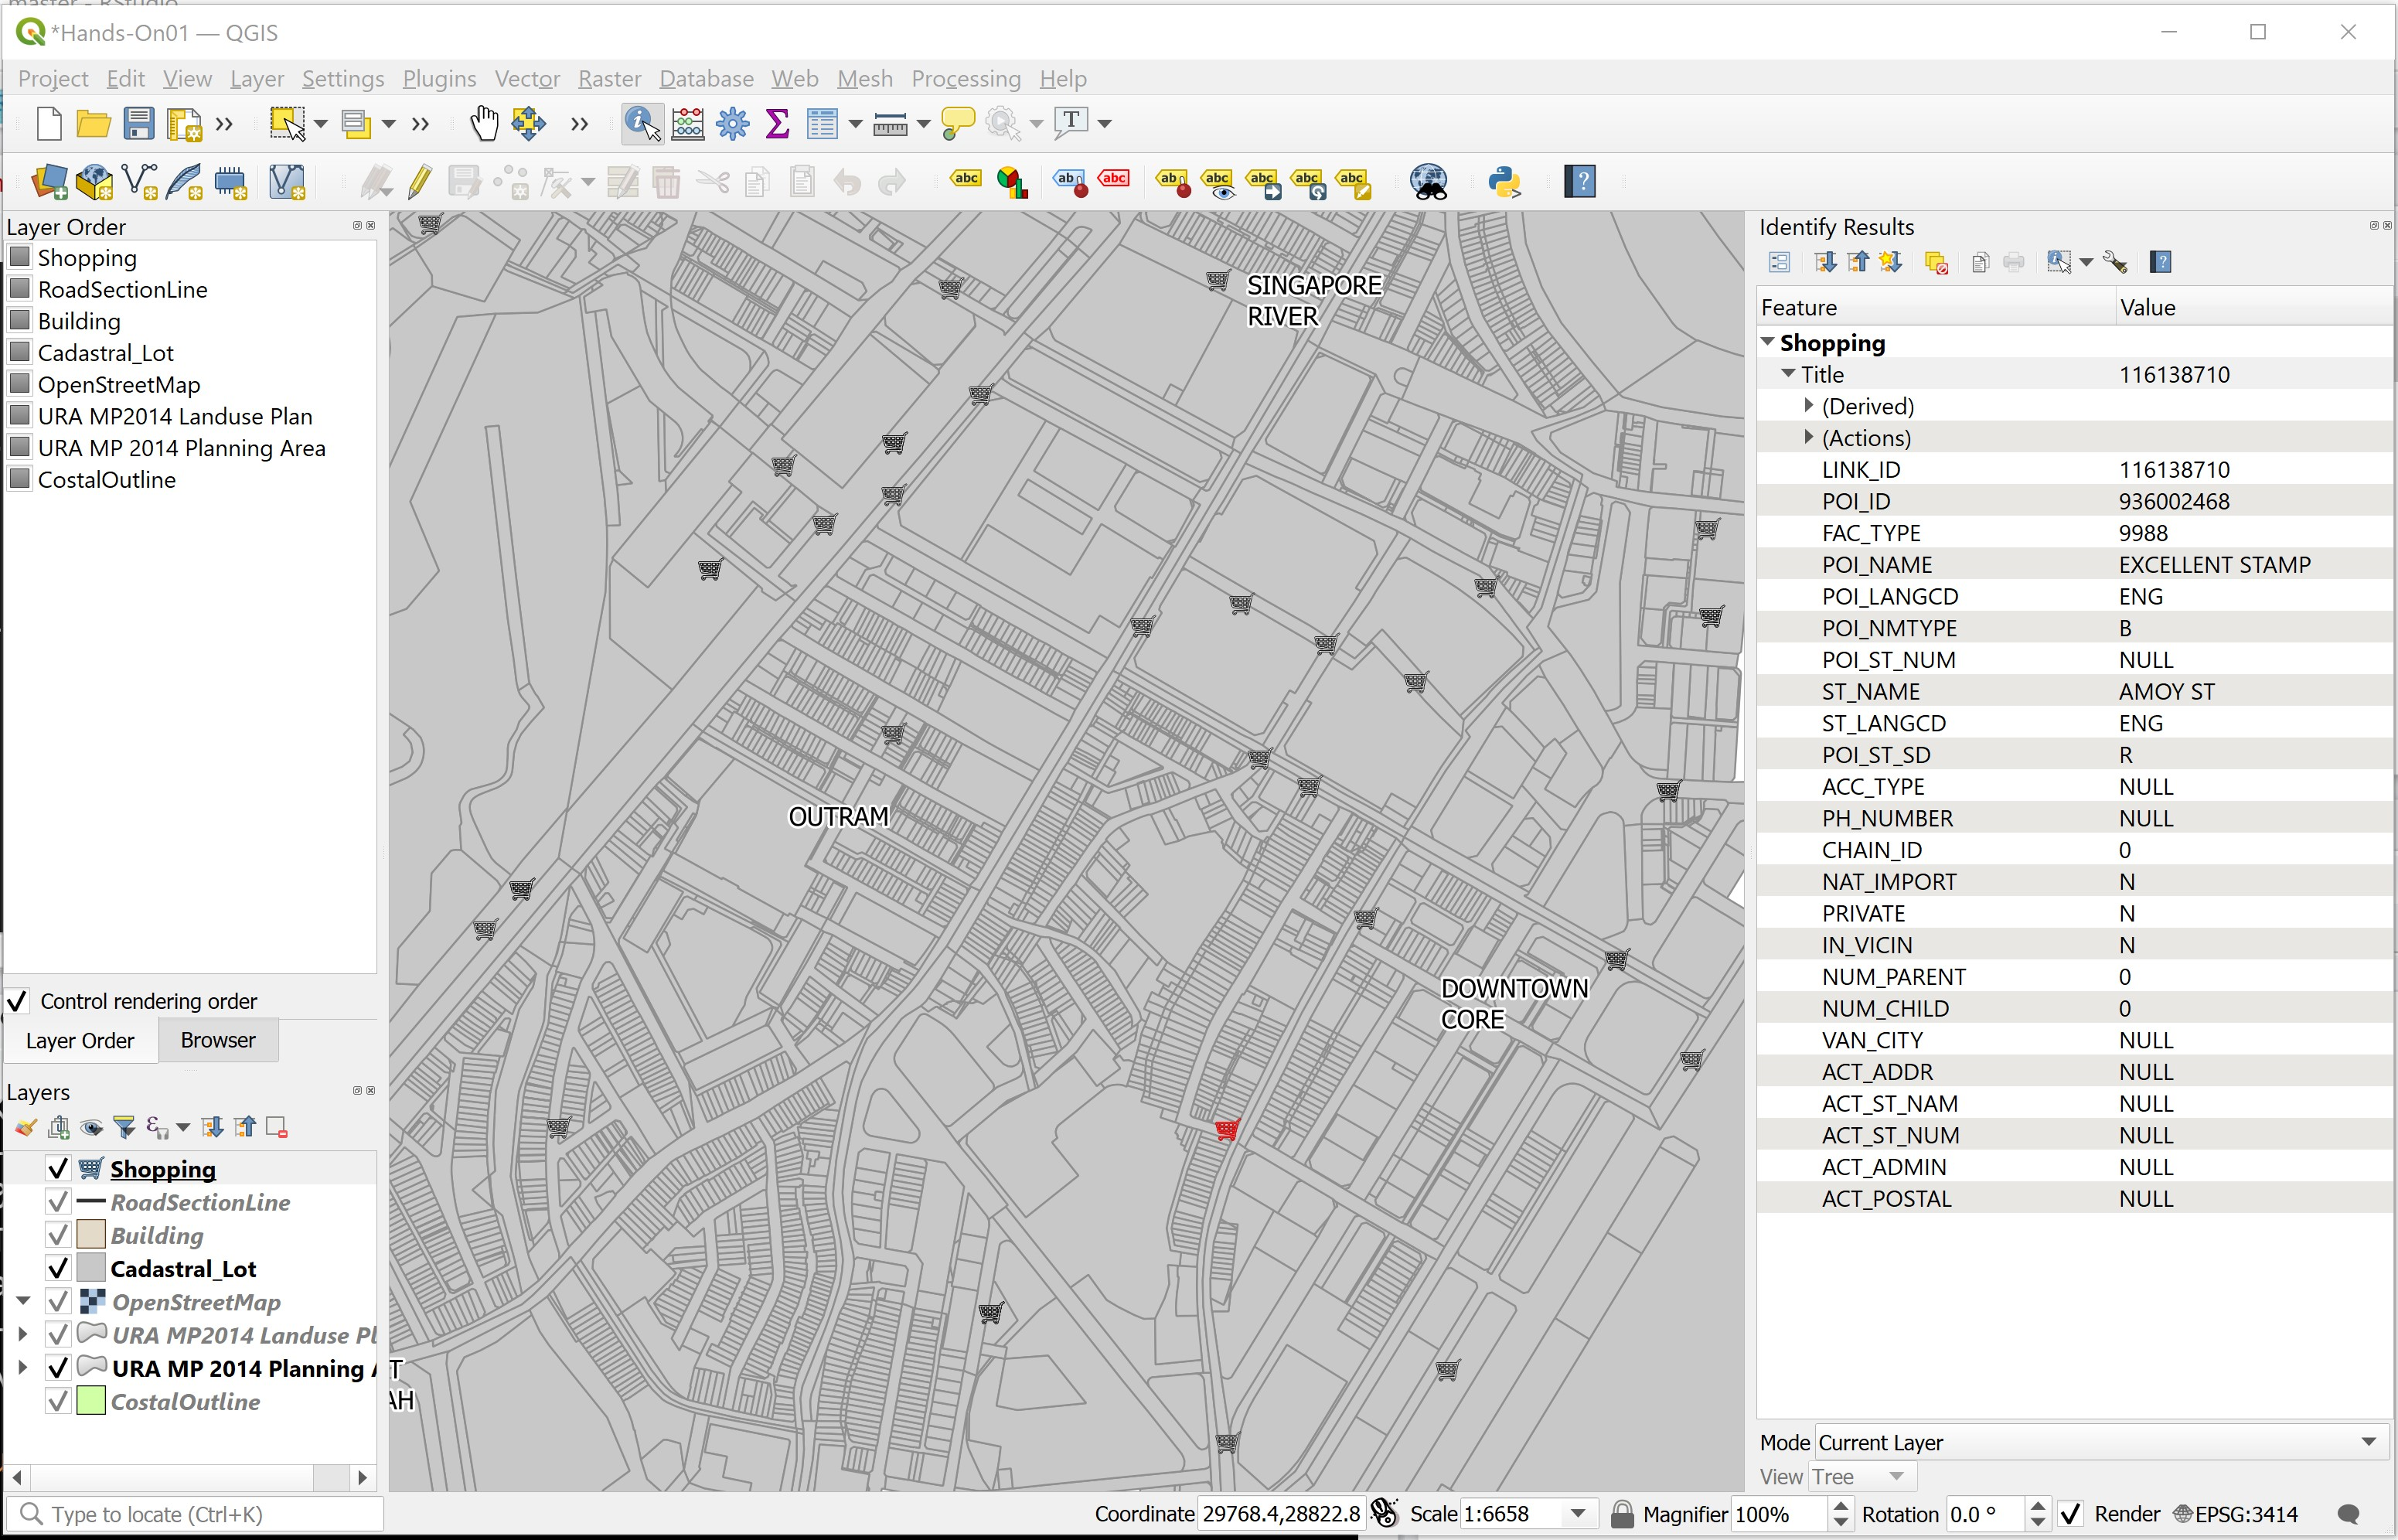
\includegraphics{./img/image1-21.jpg}

Notice that the selected shopping feature was highlighted (i.e.~in red)
and the Identify Results window appears.

\begin{quote}
DIY: Using the steps you had learned from this section, query a building
feature, a road network feature and a URA planning area feature.
\end{quote}

\hypertarget{query-attribute-table}{%
\subsection{Query Attribute Table}\label{query-attribute-table}}

The ability to interactively select a geographic feature and query its
associated attribute information is a very powerful feature of a GIS.
However, there are times that you would like to see the attributes of
all the features in a GIS layer. In this section, you will learn how to
use QGIS's Open Attribute Table function to display the attribute table
of a GIS layer.

• At the \textbf{Map Legend} window, right-click on \texttt{Building}
layer.

• Select \textbf{Open Attribute Table} from the context menu.

The \textbf{Attribute table} window appears.

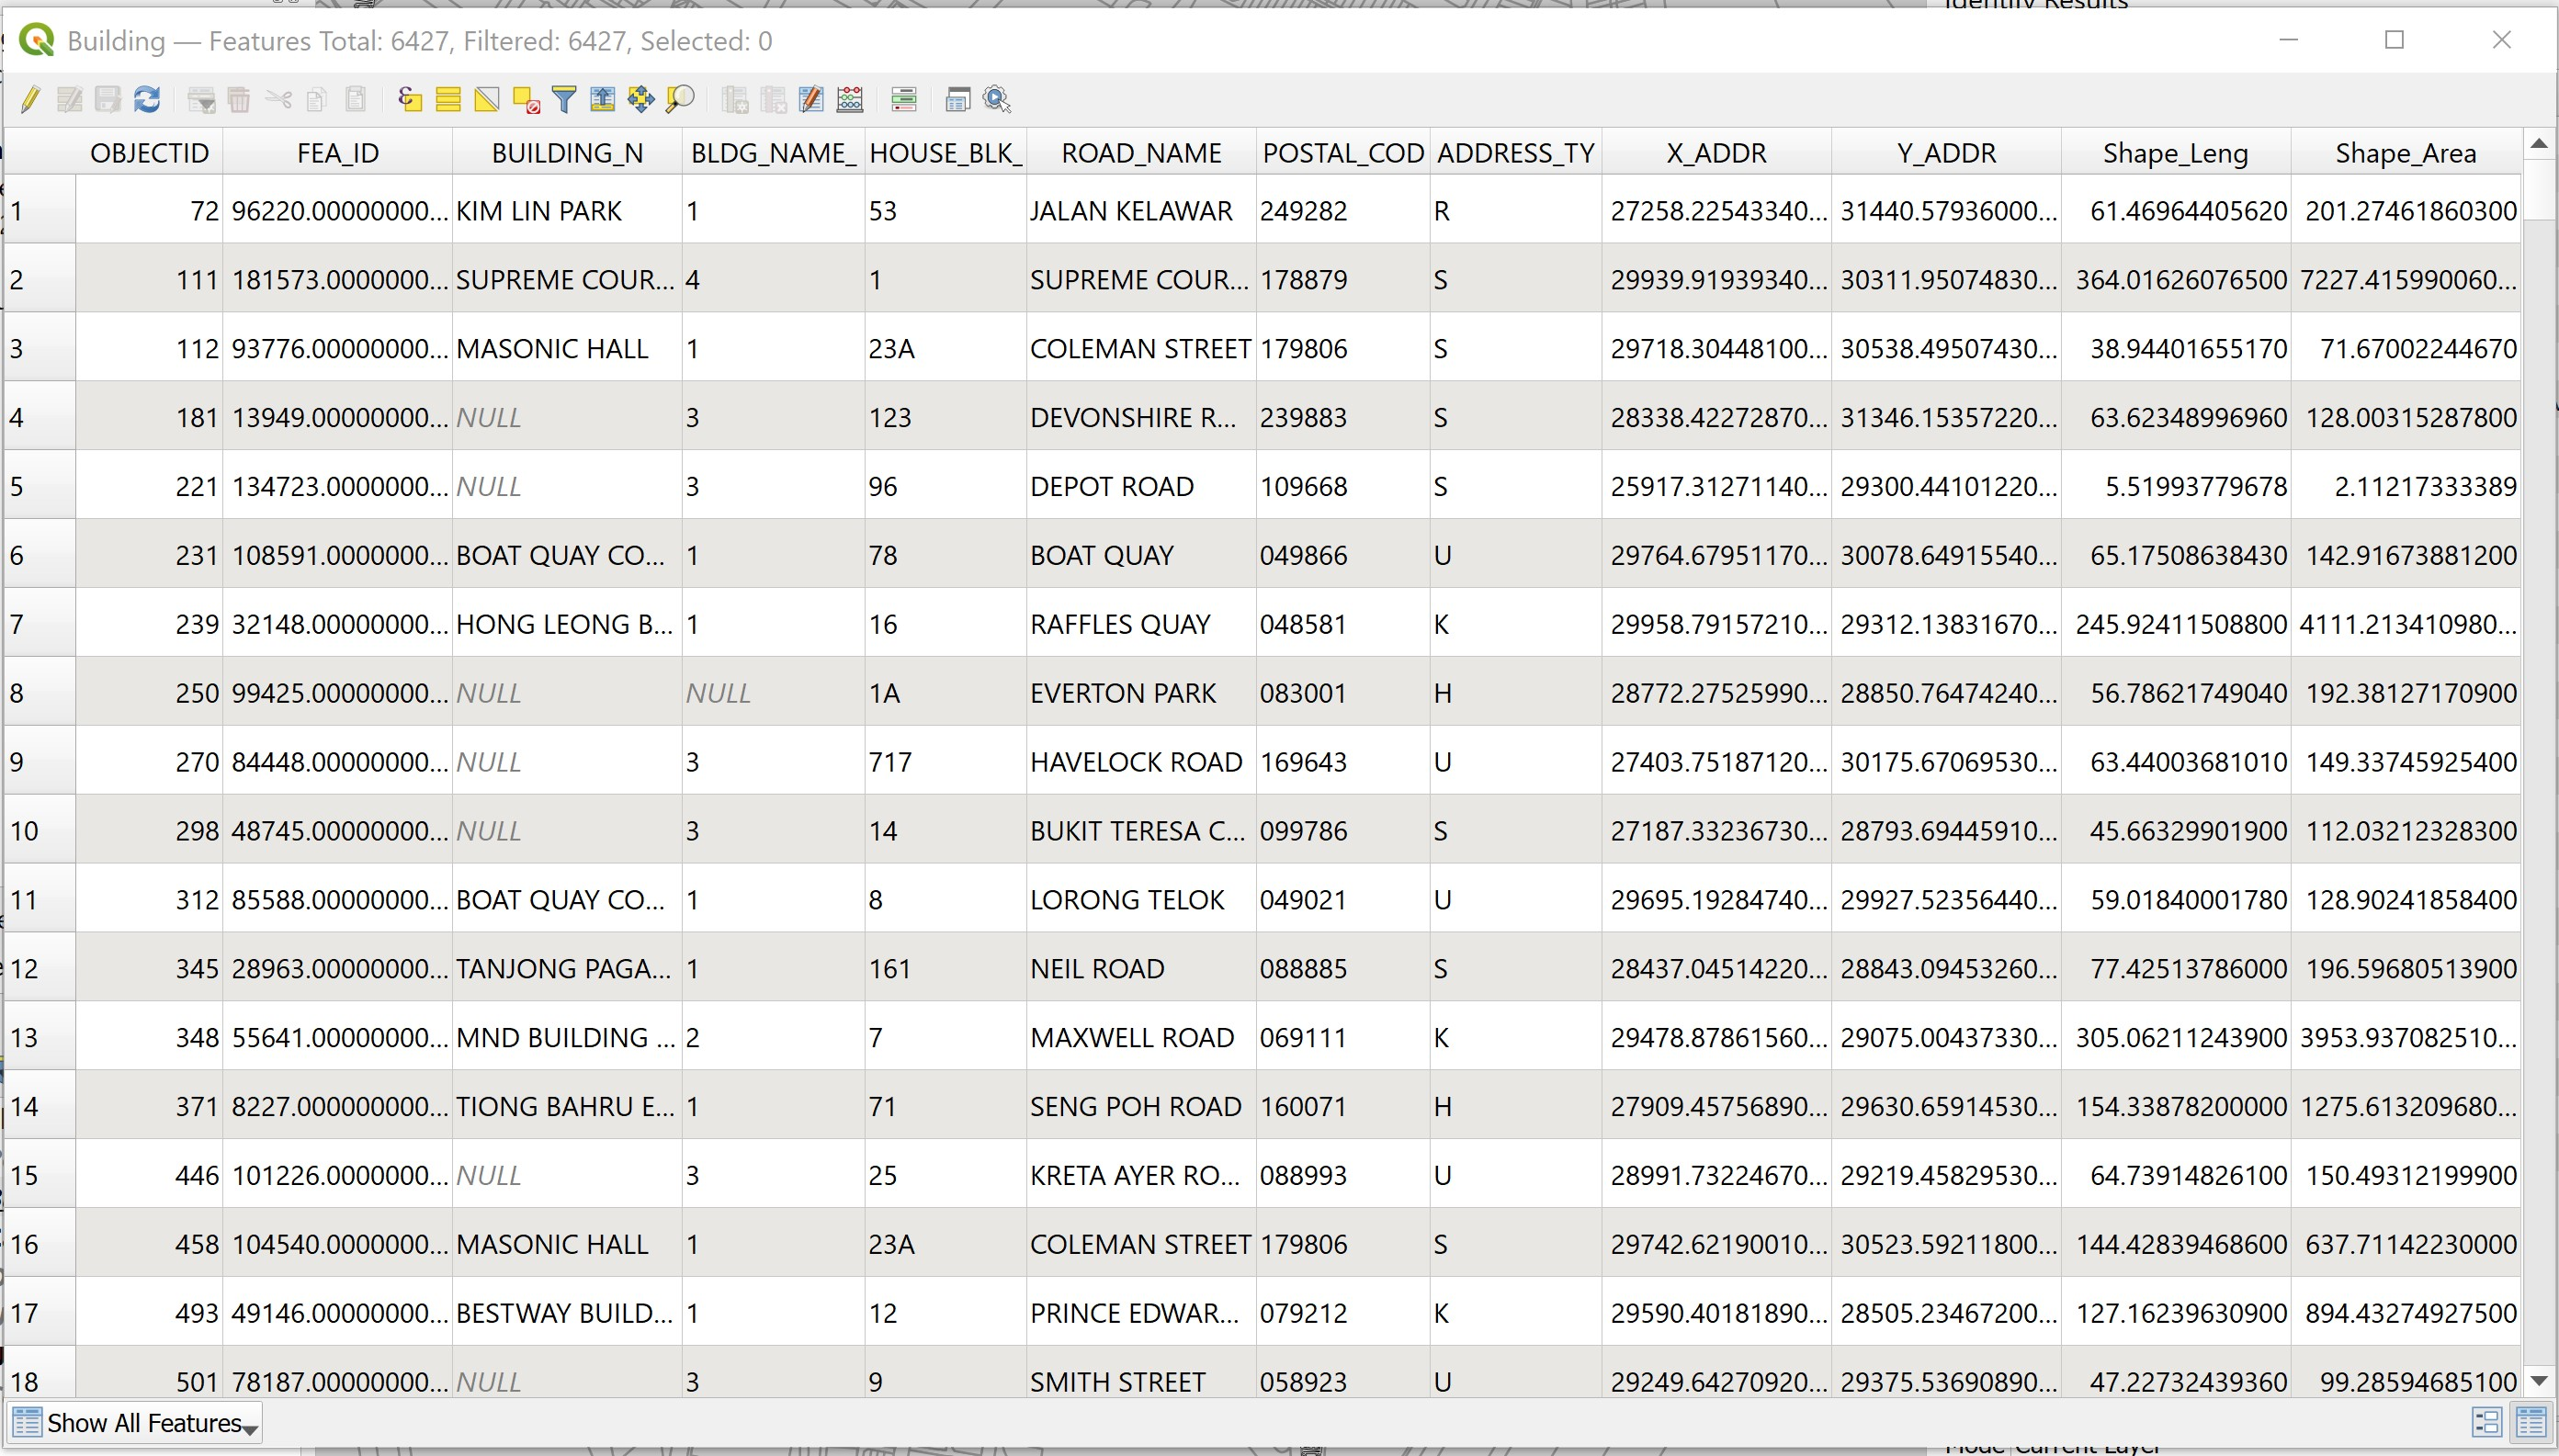
\includegraphics{./img/image1-22.jpg}

The table provide detail information of each geographical feature
(i.e.~building) such as building name, postal code, road name, block
number, just to name a few of them.

\begin{quote}
DIY: Using the steps you had learned from this section, review the
attribute table of \texttt{Shopping} and
\texttt{URA\ MP2014\ Planning\ Area} layers.
\end{quote}

\hypertarget{spatial-bookmarking}{%
\section{Spatial Bookmarking}\label{spatial-bookmarking}}

Spatial Bookmarks allow us to ``bookmark'' a geographic location and
return to it later. In this sub-section, you will learn how to create a
spatial bookmark. You will also learn how to navigate using spatial
bookmark.

\hypertarget{create-spatial-bookmark}{%
\subsection{Create spatial bookmark}\label{create-spatial-bookmark}}

We are interested to create a bookmark for the downtown centre.

\begin{itemize}
\tightlist
\item
  At the layer panel, right click on \texttt{Cadastral\ Lot}, select
  \textbf{Zoom to Layer(s)} from the context menu.*
\end{itemize}

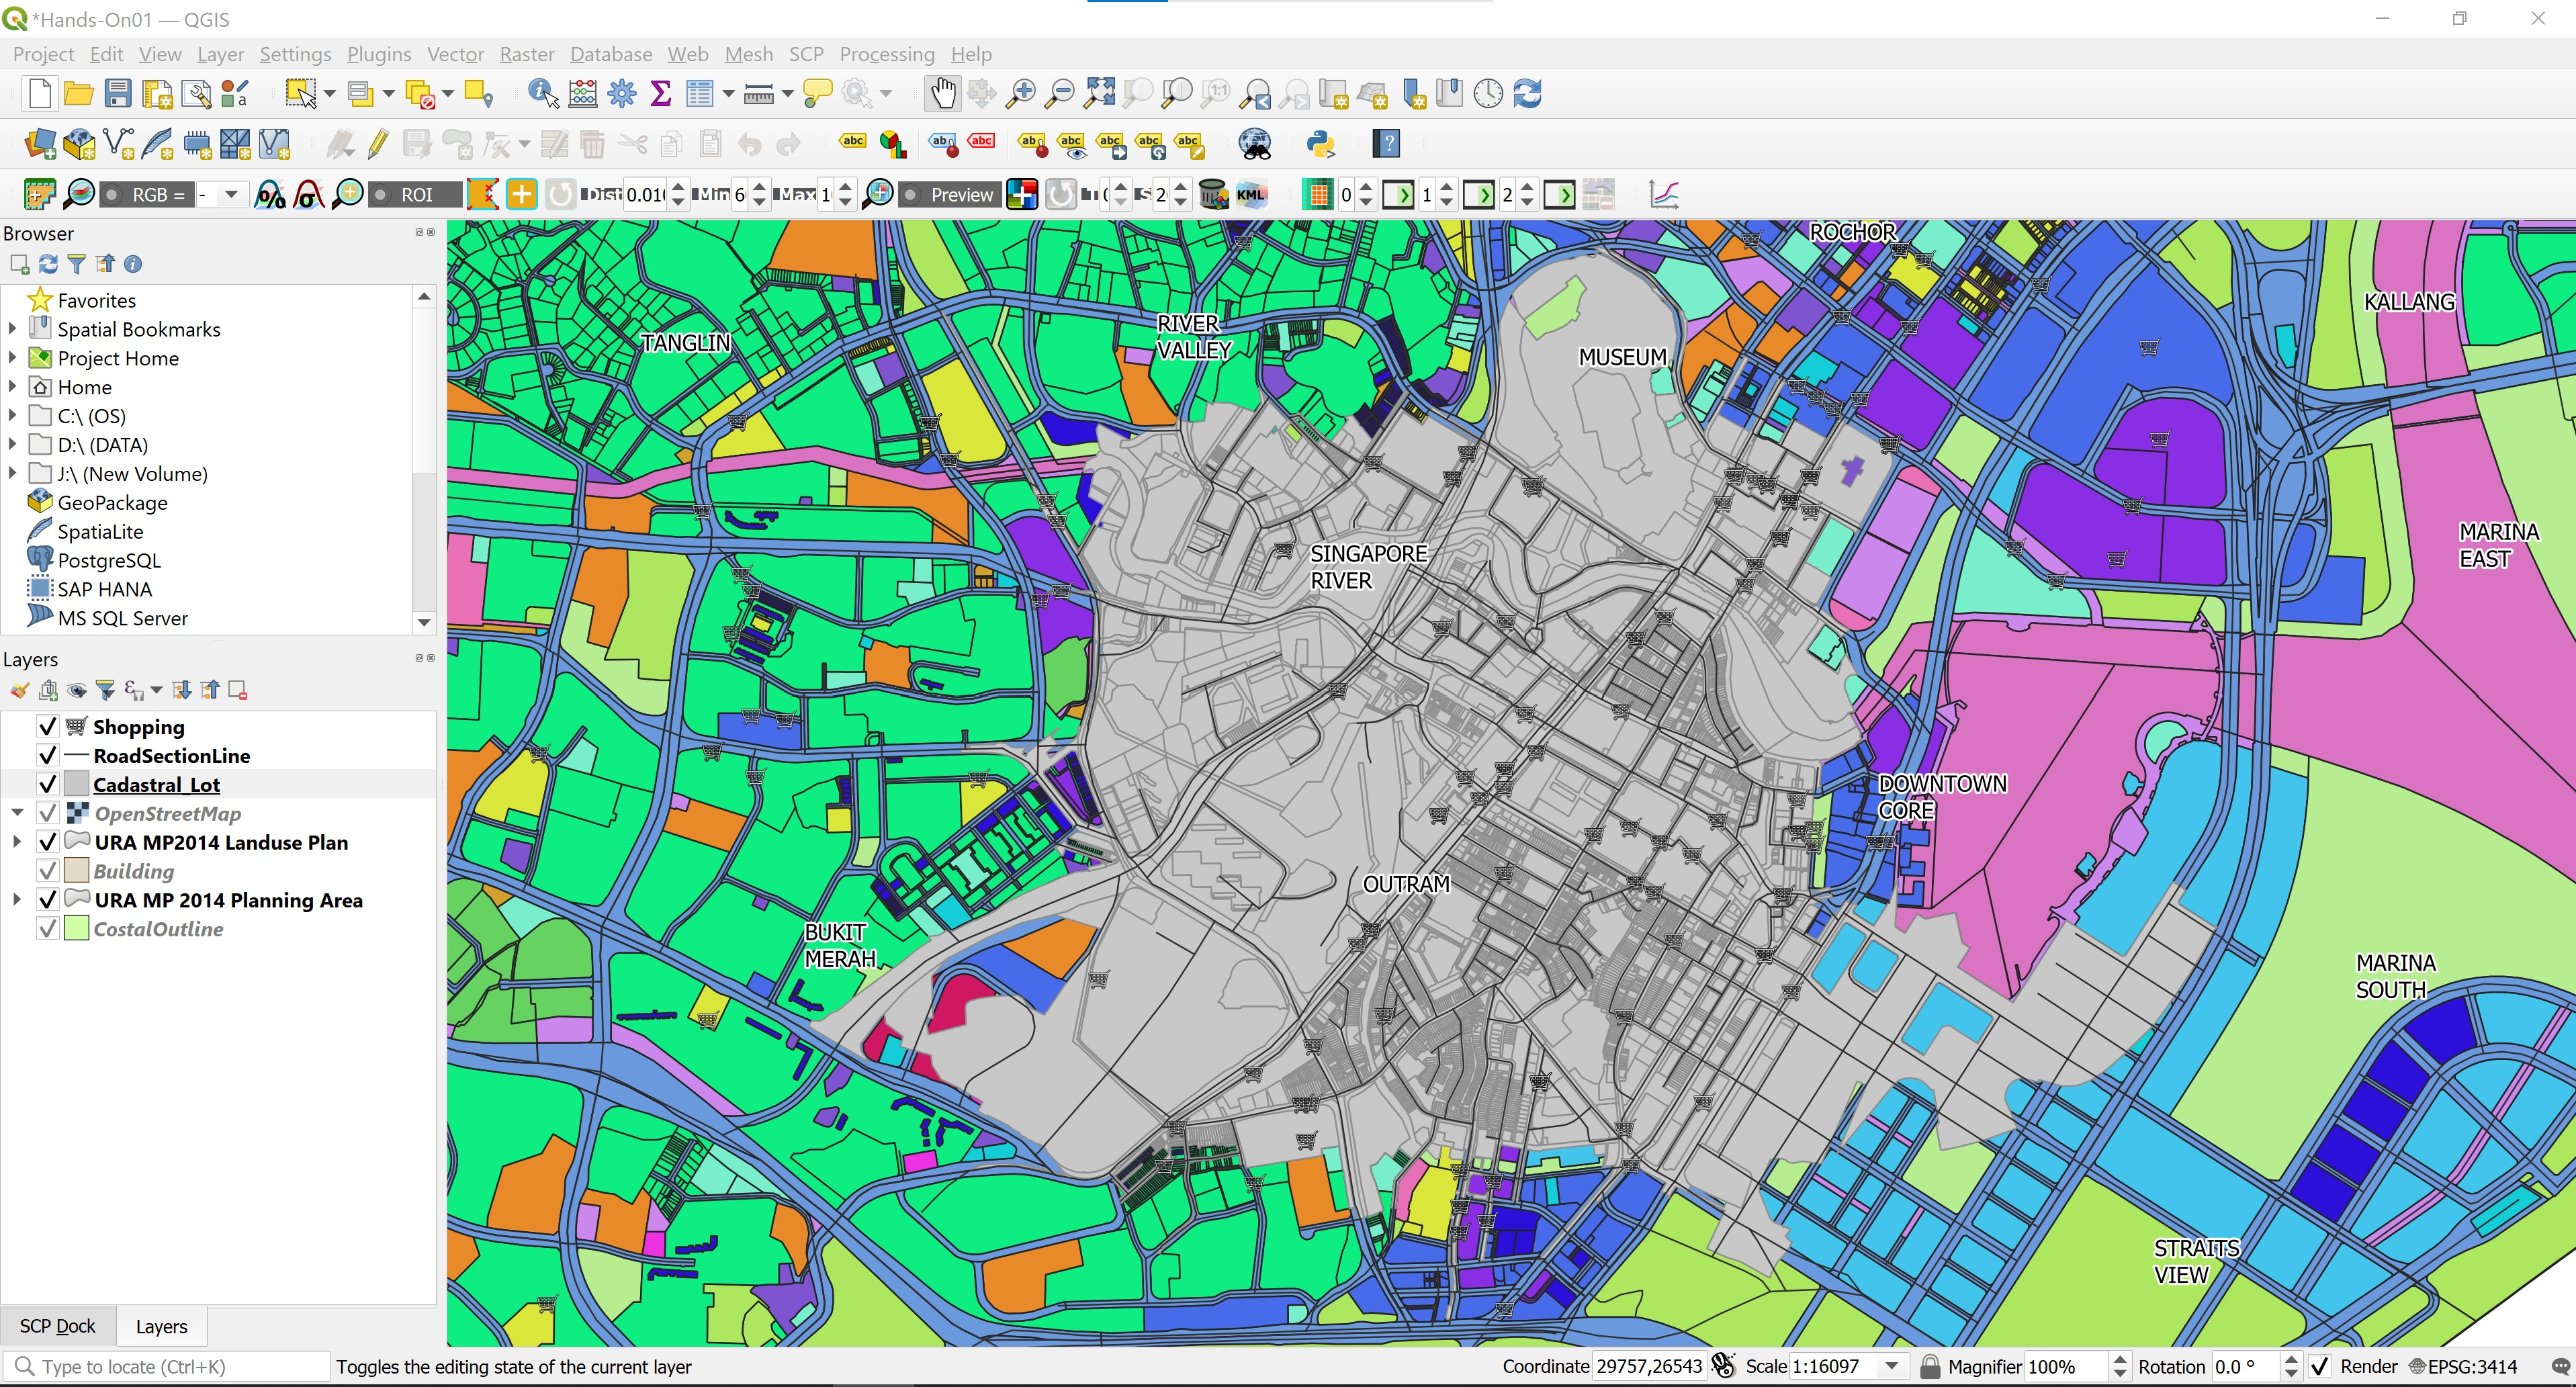
\includegraphics{./img02/image31.jpg}

\begin{itemize}
\tightlist
\item
  From the menu bar, click on \textbf{View} -\textgreater{} \textbf{New
  Spatial Boomark}.
\end{itemize}

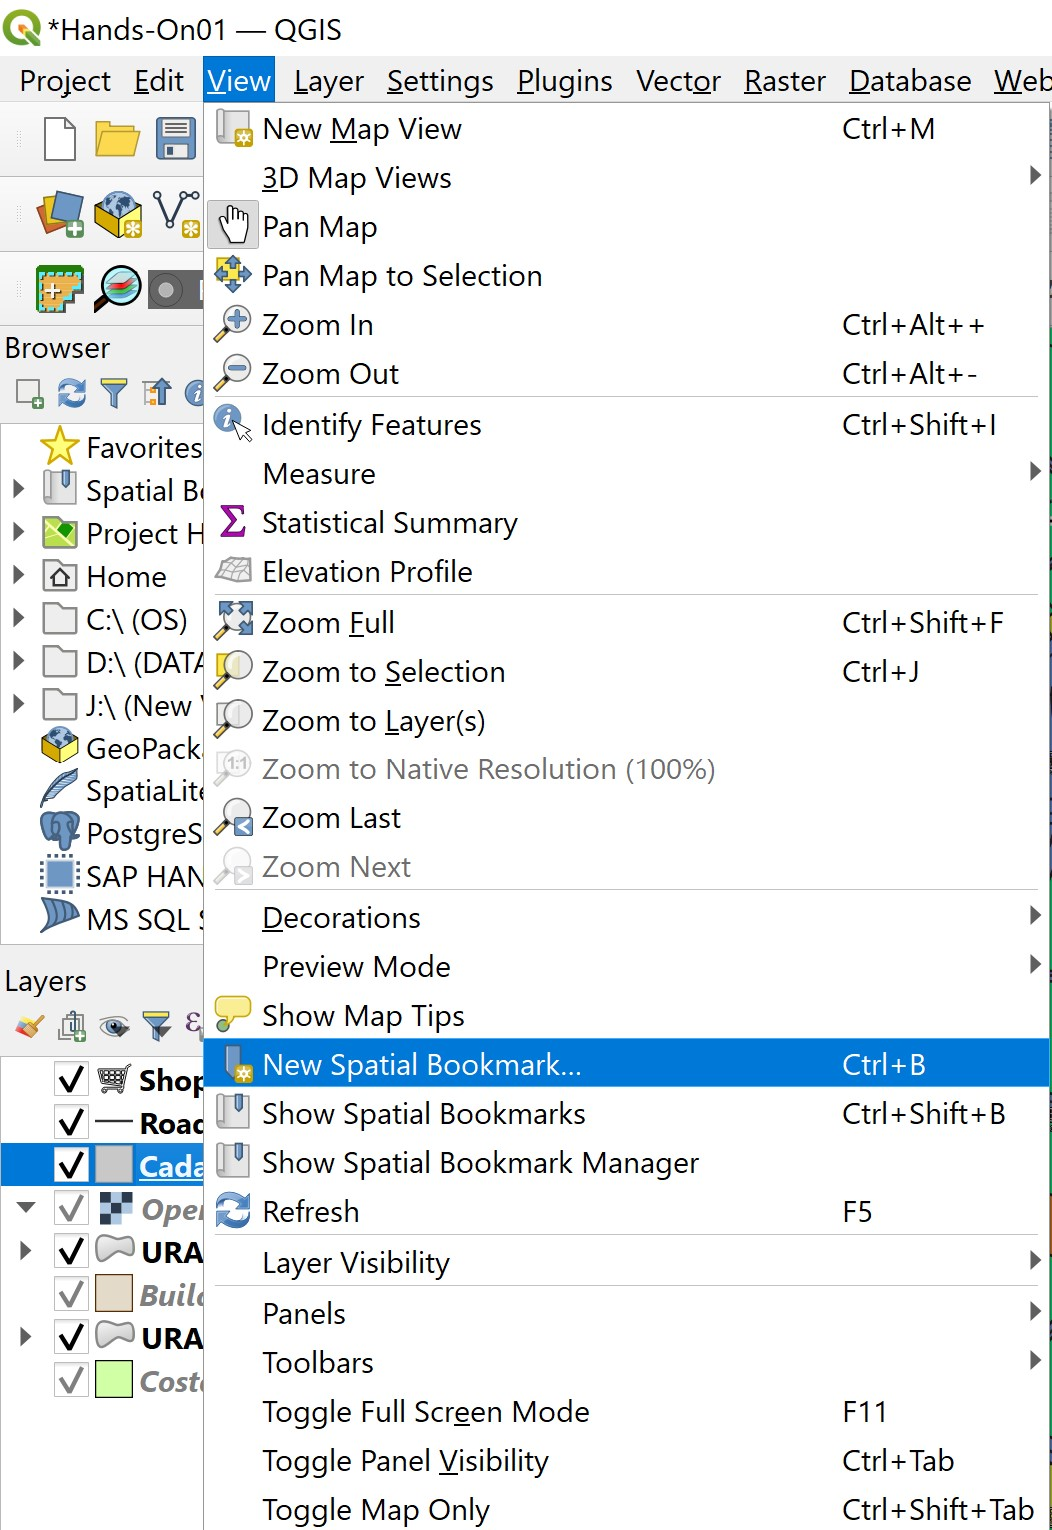
\includegraphics[width=3.75in,height=\textheight]{./img02/image32.jpg}

Bookmark Editor dialog window appears.

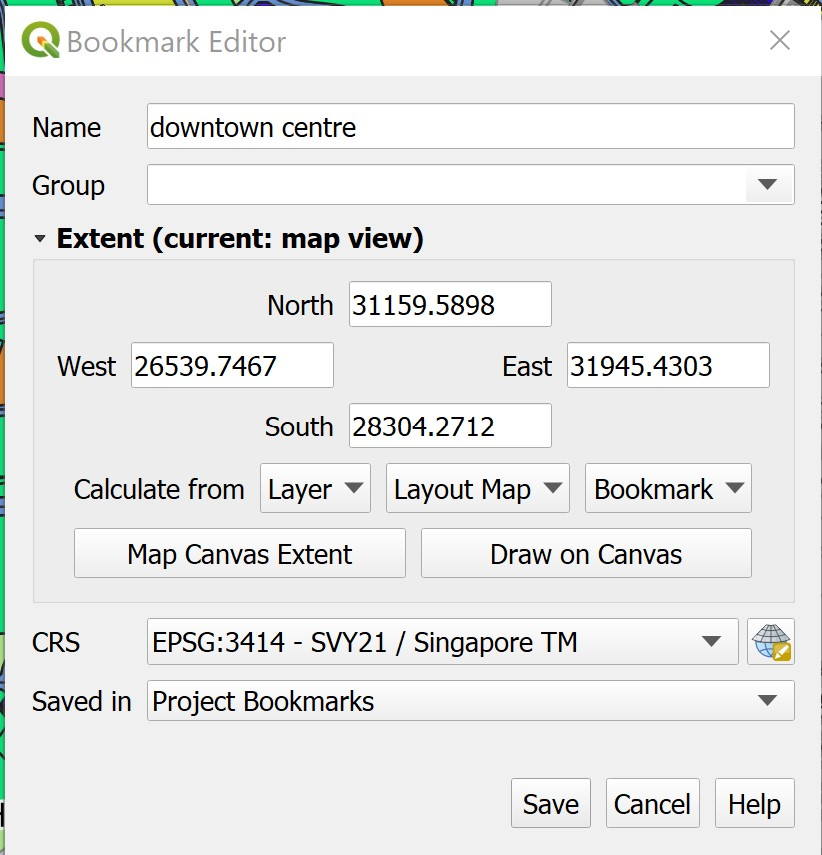
\includegraphics[width=3.125in,height=\textheight]{./img02/image33.jpg}

\begin{itemize}
\item
  For \textbf{Name:}, type \texttt{downtown\ centre}.
\item
  For \textbf{Save in}, select \textbf{Project Bookmarks} from the
  dropdown list. This will save the spatial bookmark in the project
  file.
\item
  Click \textbf{Save} button.
\end{itemize}

Now, you are ready to test if the newly create spatial bookmark works
correctly.

First, we will zoom out to the extend of planning area.

\begin{quote}
DIY: Using the steps you had learned from earlier section,zoom to the
extend of \texttt{URA\ MP\ 2014\ Planning\ Area} layer.
\end{quote}

\begin{itemize}
\tightlist
\item
  From the menu bar select \textbf{View} -\textgreater{} \textbf{Show
  Spatial Bookmarks}.
\end{itemize}

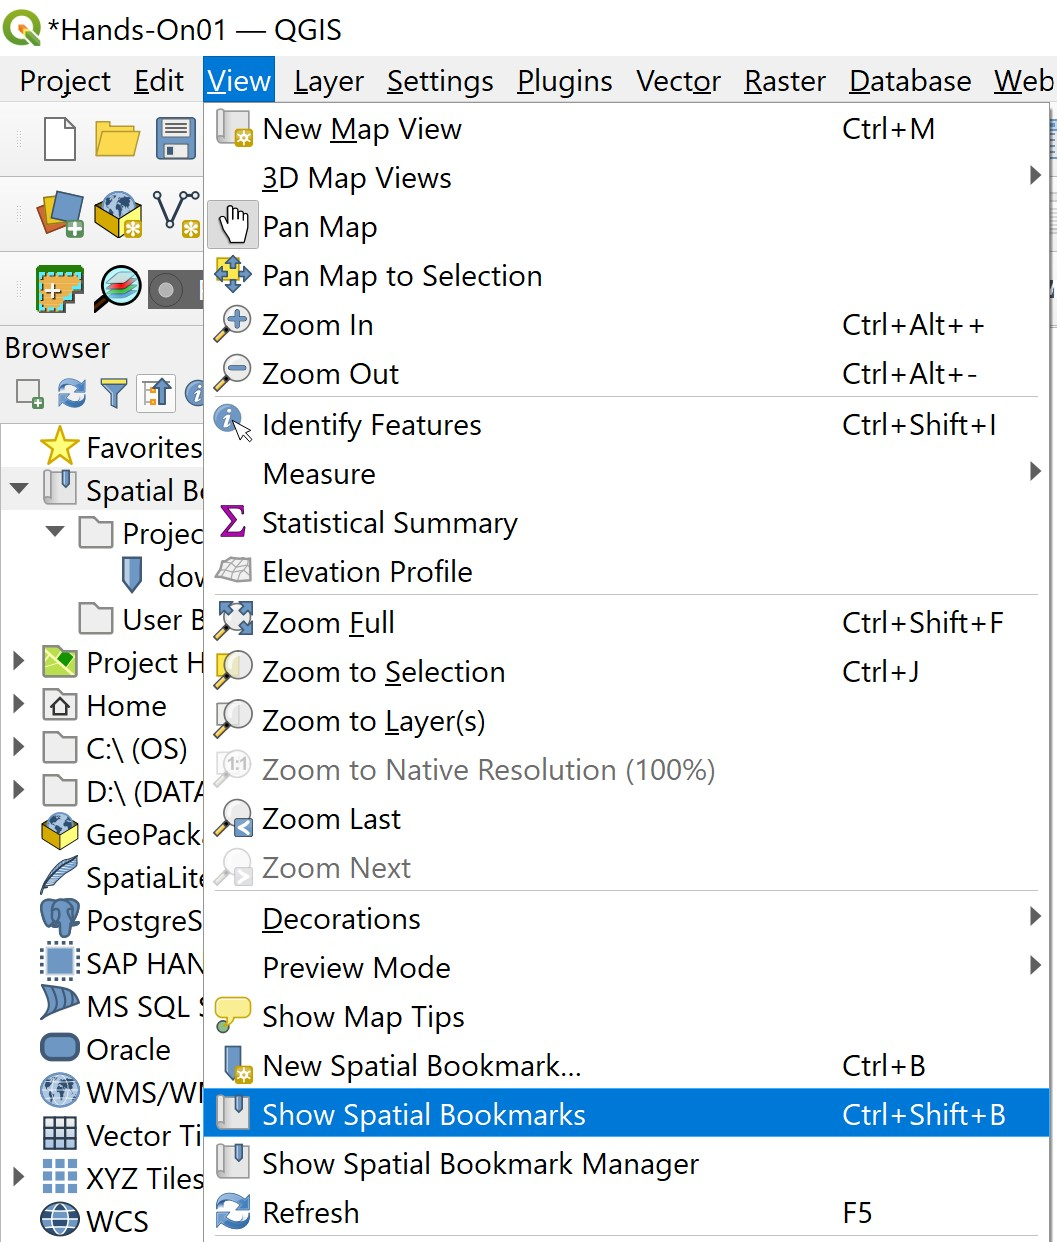
\includegraphics[width=3.75in,height=\textheight]{./img02/image34.jpg}

Notice that a new item call Spatial Bookmarks is added on the Browser
pane as shown in the screenshot below.

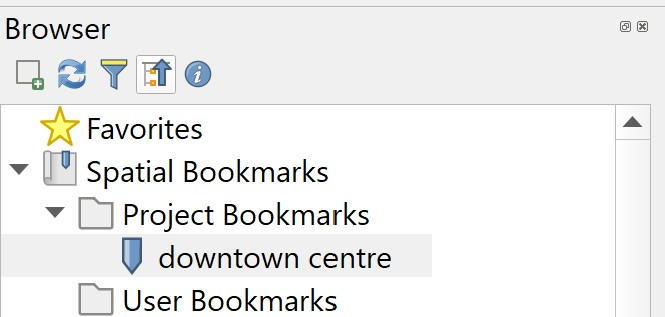
\includegraphics[width=3.04167in,height=\textheight]{./img02/image35.jpg}

\begin{itemize}
\tightlist
\item
  Double-click on downtown centre.
\end{itemize}

Notice that the view will zoom to the same map extend centre at the
Downtown Centre you have saved as spatial bookmark not long ago.

\begin{quote}
DIY: Choose a planning area i.e.~Choa Chu Kang. Next, using the steps
you had learned from earlier section, create a new spatial bookmark.
\end{quote}

Whew! That was a lot to take in! Take a deep breath and relax. By now
you should have a good understanding of the basic operations of QGIS.
You can start playing with it and practice the techniques that you have
learned.

\bookmarksetup{startatroot}

\hypertarget{working-with-gis-data}{%
\chapter{Working with GIS Data}\label{working-with-gis-data}}

A GIS is specially designed to manage geospatial data. This hands-on
exercise consists of five sections. First, you will learn how to import
geospatial data from different sources and file format into QGIS. At the
same time, you will also learn how to check their feature type,
coordinate system and other related information. You will also learn how
to create a GIS data from an aspatial data by using QGIS. Next, you will
learn how to transform this newly created GIS layer into Singapore
National projected coordinates systems (i.e.~SVY21). Lastly, you will
also learn how to use the geocoding function of QGIS to create
geospatially referenced data from a non-spatial data.

\hypertarget{learning-outcome}{%
\section{Learning Outcome}\label{learning-outcome}}

By the end of this session, you will be able to:

\begin{itemize}
\tightlist
\item
  work with geospatial data from data.gov.sg
\item
  create geospatially-enabled data
\item
  create GIS Layer from a text data with georeference information
\item
  transform a GIS data onto a different projection system
\item
  work with raster GIS data • work with internet geospatial services •
  work with geospatial database
\end{itemize}

\hypertarget{working-with-geospatial-data-from-data.gov.sg}{%
\section{Working with Geospatial Data from
data.gov.sg}\label{working-with-geospatial-data-from-data.gov.sg}}

In this section, you will learn how to download geospatial data from
data.gov.sg and import them into QGIS.

\hypertarget{downloading-geospatial-data-from-data.gov.sg}{%
\subsection{Downloading geospatial data from
data.gov.sg}\label{downloading-geospatial-data-from-data.gov.sg}}

First, you are required to download the following geospatial and
aspatial data from \href{https://data.gov.sg/}{data.gov.sg}:

\begin{itemize}
\tightlist
\item
  Master Plan 2014 Subzone Boundary (No Sea),
\item
  Child Care Services,
\item
  Street and Places, and
\item
  School Directory and Information
\end{itemize}

\hypertarget{managing-the-imported-data}{%
\subsection{Managing the imported
data}\label{managing-the-imported-data}}

For any GIS project, it is important for us to practice good document
management. Assuming that the root directory of this project is called
\texttt{Hands-on\_Ex02},

\begin{itemize}
\tightlist
\item
  created a sub-folder call \texttt{data.gov}.\\
\item
  inside \texttt{data.gov}, create two new sub-folders. Call them
  \texttt{geospatial} and \texttt{aspatial} respectively.
\item
  place the downloaded Master Plan 2014 Subzone Boundary (No Sea), Child
  Care Services and Street and Places into the geospatial folder.

  \begin{itemize}
  \tightlist
  \item
    unzipped their respective zipped files,
  \item
    extract the unzipped files, and
  \item
    place them in \texttt{geospatial} folder.
  \end{itemize}
\item
  place the downloaded School Directory and Information zipped file into
  aspatial sub-folder.

  \begin{itemize}
  \tightlist
  \item
    unzipped the file,
  \item
    copy and paste \texttt{general-information-of-schools.csv} into
    \texttt{aspatial} sub-folder.
  \end{itemize}
\end{itemize}

The geospatial folder should look similar to the screenshot below.

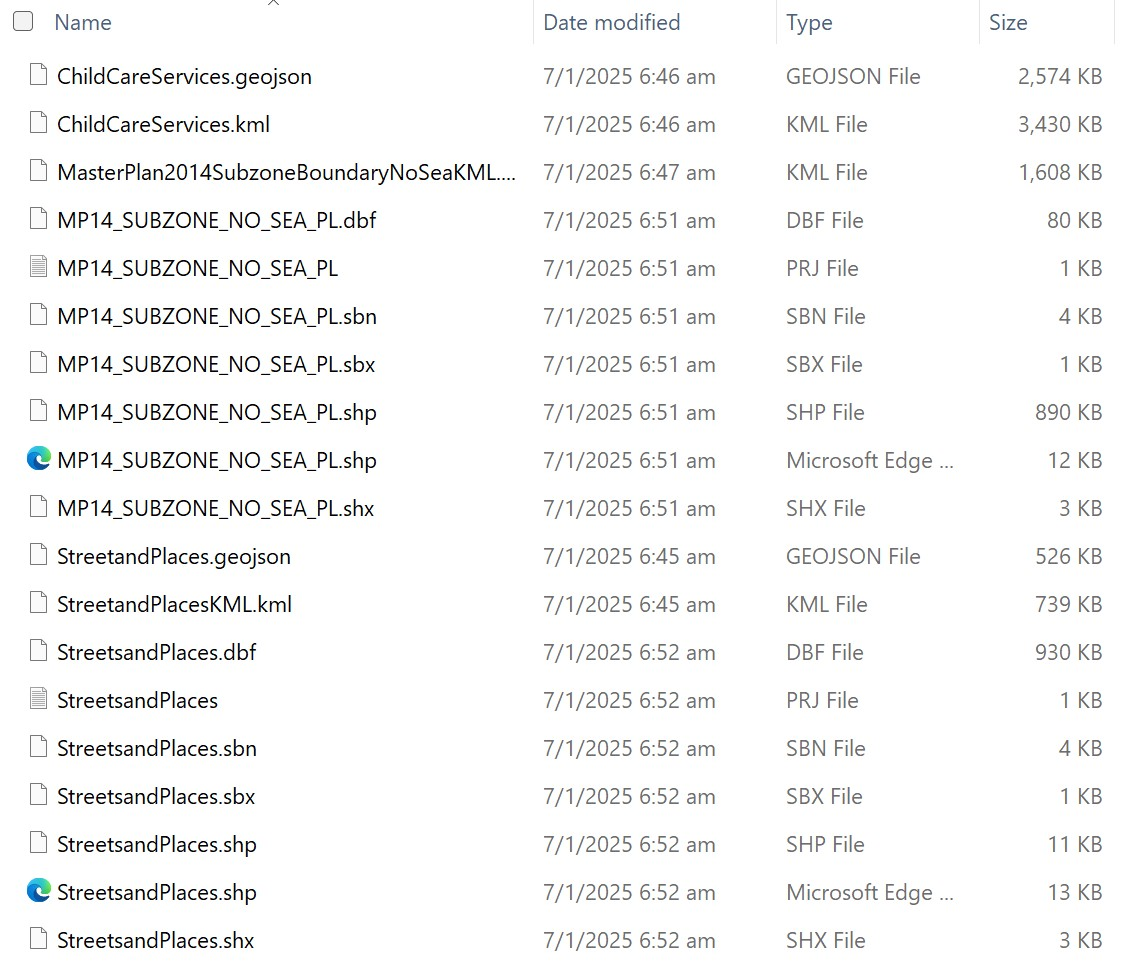
\includegraphics{./img02/image1.jpg}

Notice that besides the geospatial data files, I also include the
metadata of the data into the folder. This is because the metadata
provide useful information of the data and it is important for us to
keep them for future references.

\hypertarget{examining-the-geospatial-data}{%
\subsection{Examining the geospatial
data}\label{examining-the-geospatial-data}}

Before you add the GIS data into QGIS, you should spend some time to
examine the files in \texttt{geospatial} folder.

Notice that the shapefile version of MP14\_SUBZONE\_NO\_SEA\_PL and
StreetsandPlaces data sets are actually made up of multiples files that
have the same names but with different extensions.

Table below details the meaning of each file.
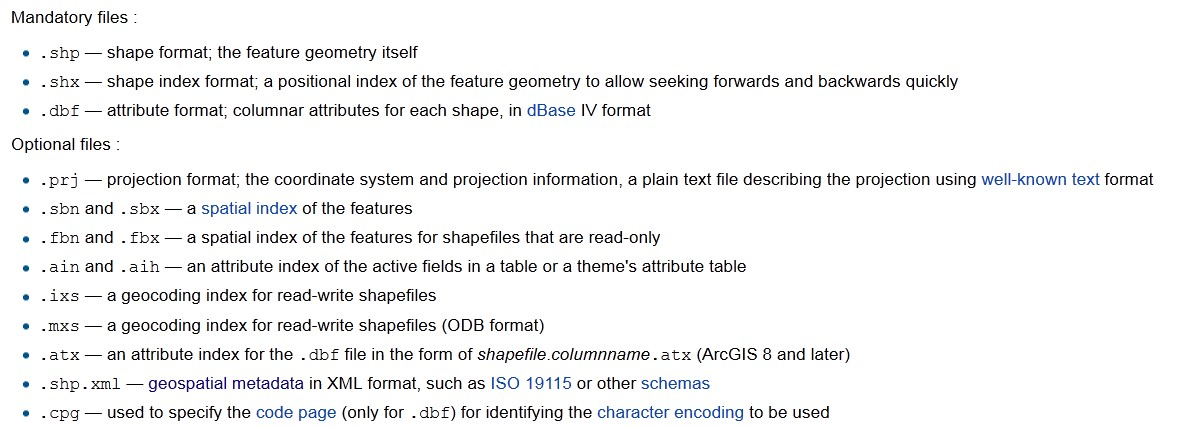
\includegraphics{./img02/image2.jpg} Source:
https://en.wikipedia.org/wiki/Shapefile

Next, you should also check the projection of the shapefile.

\begin{itemize}
\tightlist
\item
  Right-click on the PRJ file of \texttt{MP14\_SUBZONE\_NO\_SEA\_PL}
\item
  Select \emph{Open with} -\textgreater{} \emph{NotePad}.
\end{itemize}

Your NotePad should look similar to the figure below.

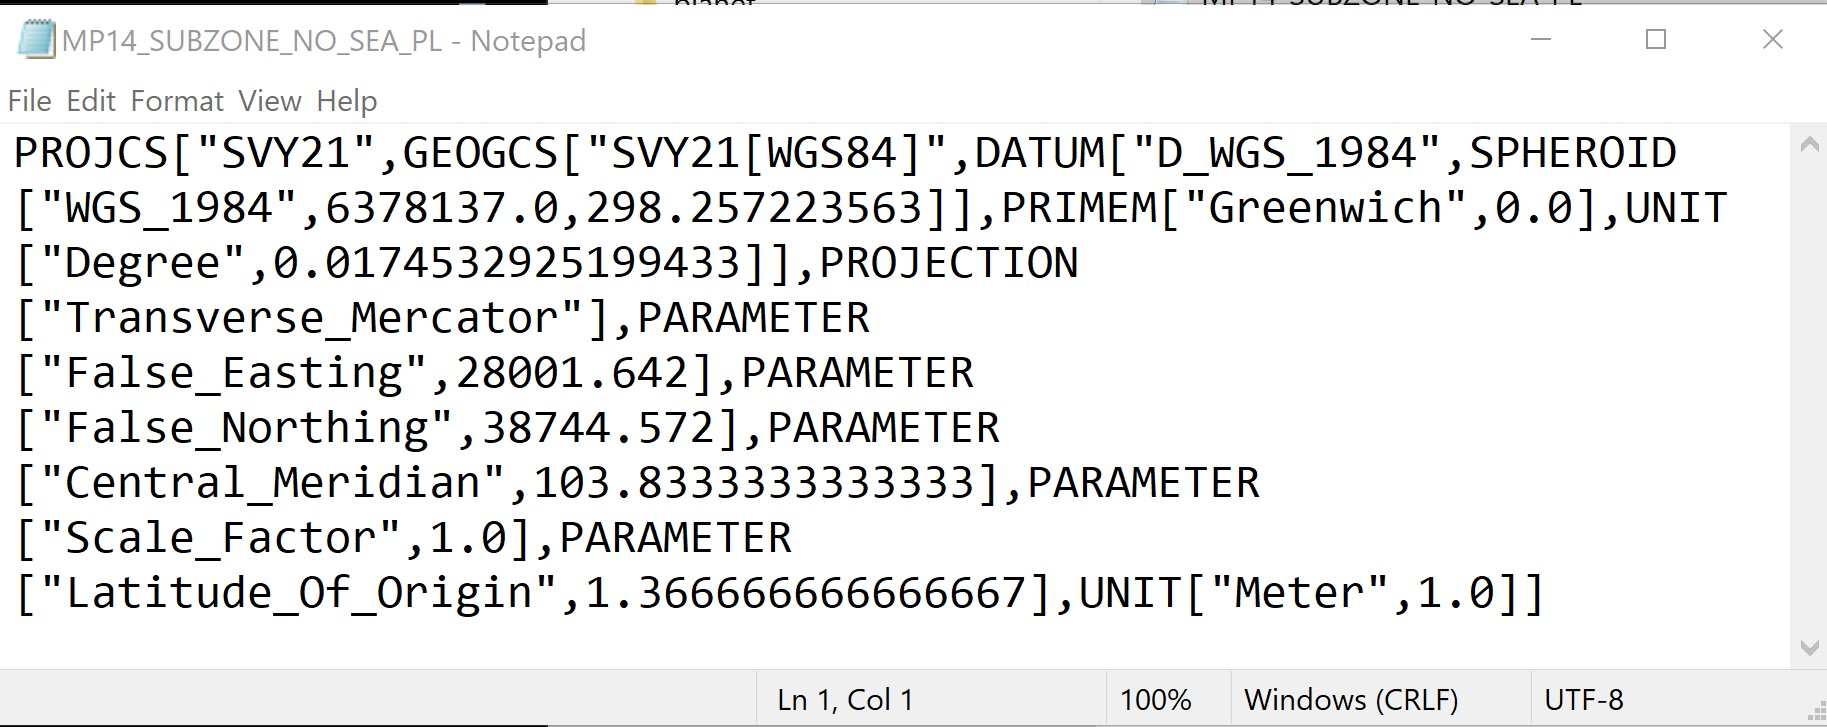
\includegraphics{./img02/image3.jpg}

From the screenshot, it is clear that
\texttt{MP14\_SUBZONE\_NO\_SEA\_PL} is in svy21 projected coordinate
system.

\begin{itemize}
\tightlist
\item
  Close the NotePad.
\end{itemize}

Different from shapefile, the geojson and kml files are editing in xml
format. You can examine the content of these two files by using either
Notepad or WordPad.

\hypertarget{adding-geospatial-data-from-data.gov-into-qgis}{%
\subsection{Adding geospatial data from data.gov into
QGIS}\label{adding-geospatial-data-from-data.gov-into-qgis}}

Now, we are ready to bring the geospatial data downloaded from
data.giv.sg into QGIS.

\begin{itemize}
\tightlist
\item
  From Window Desktop, launch QGIS.
\end{itemize}

You will start a new QGIS project.

\begin{itemize}
\tightlist
\item
  From the menu bar, select \textbf{Project} -\textgreater{}
  \textbf{New}.
\end{itemize}

Next, you are going to learn how to bring geospatial data sets into QGIS
via the \textbf{Browser} panel.

\begin{itemize}
\tightlist
\item
  From the Browser panel, navigate to the path of
  Hands-on\_Ex02\data\data.gov\geospatial as shown in the screenshot
  below.
\end{itemize}

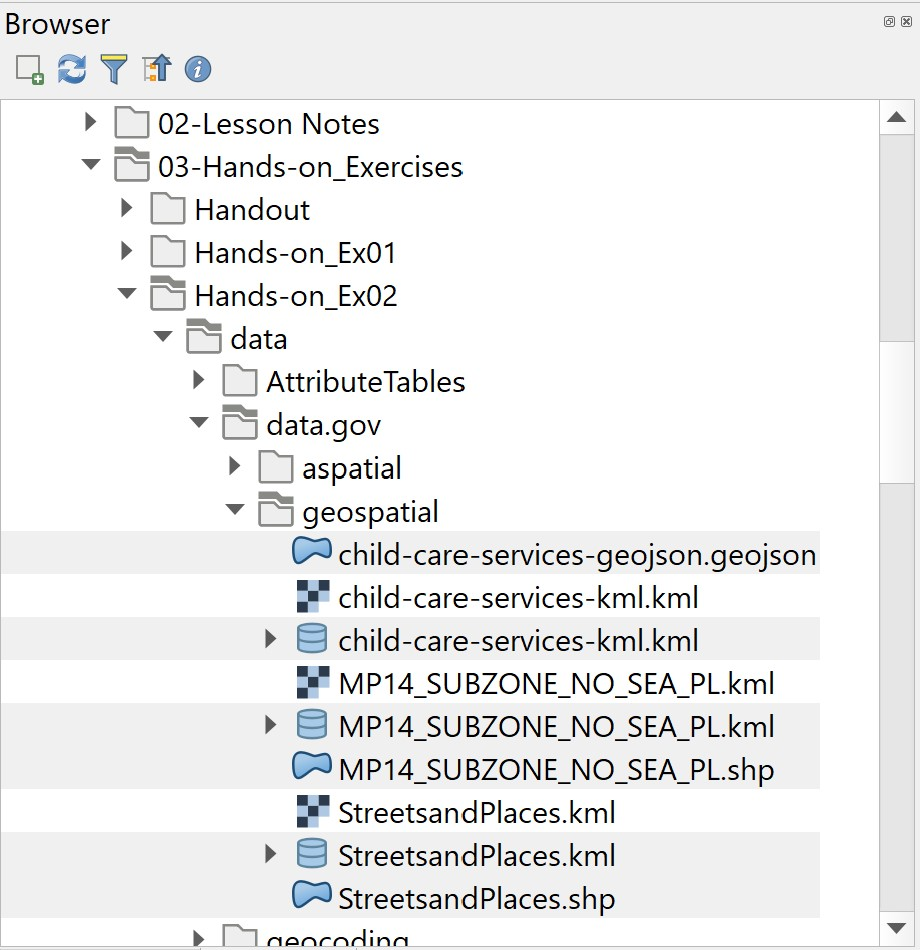
\includegraphics{./img02/image4.jpg}

\begin{itemize}
\tightlist
\item
  Double-click on \texttt{child-care-services-geojson.geojson}.
\end{itemize}

Notice that \texttt{child-care-services-geojson.geojson} is added in the
\textbf{Layer} panel and display on the View window as shown below.

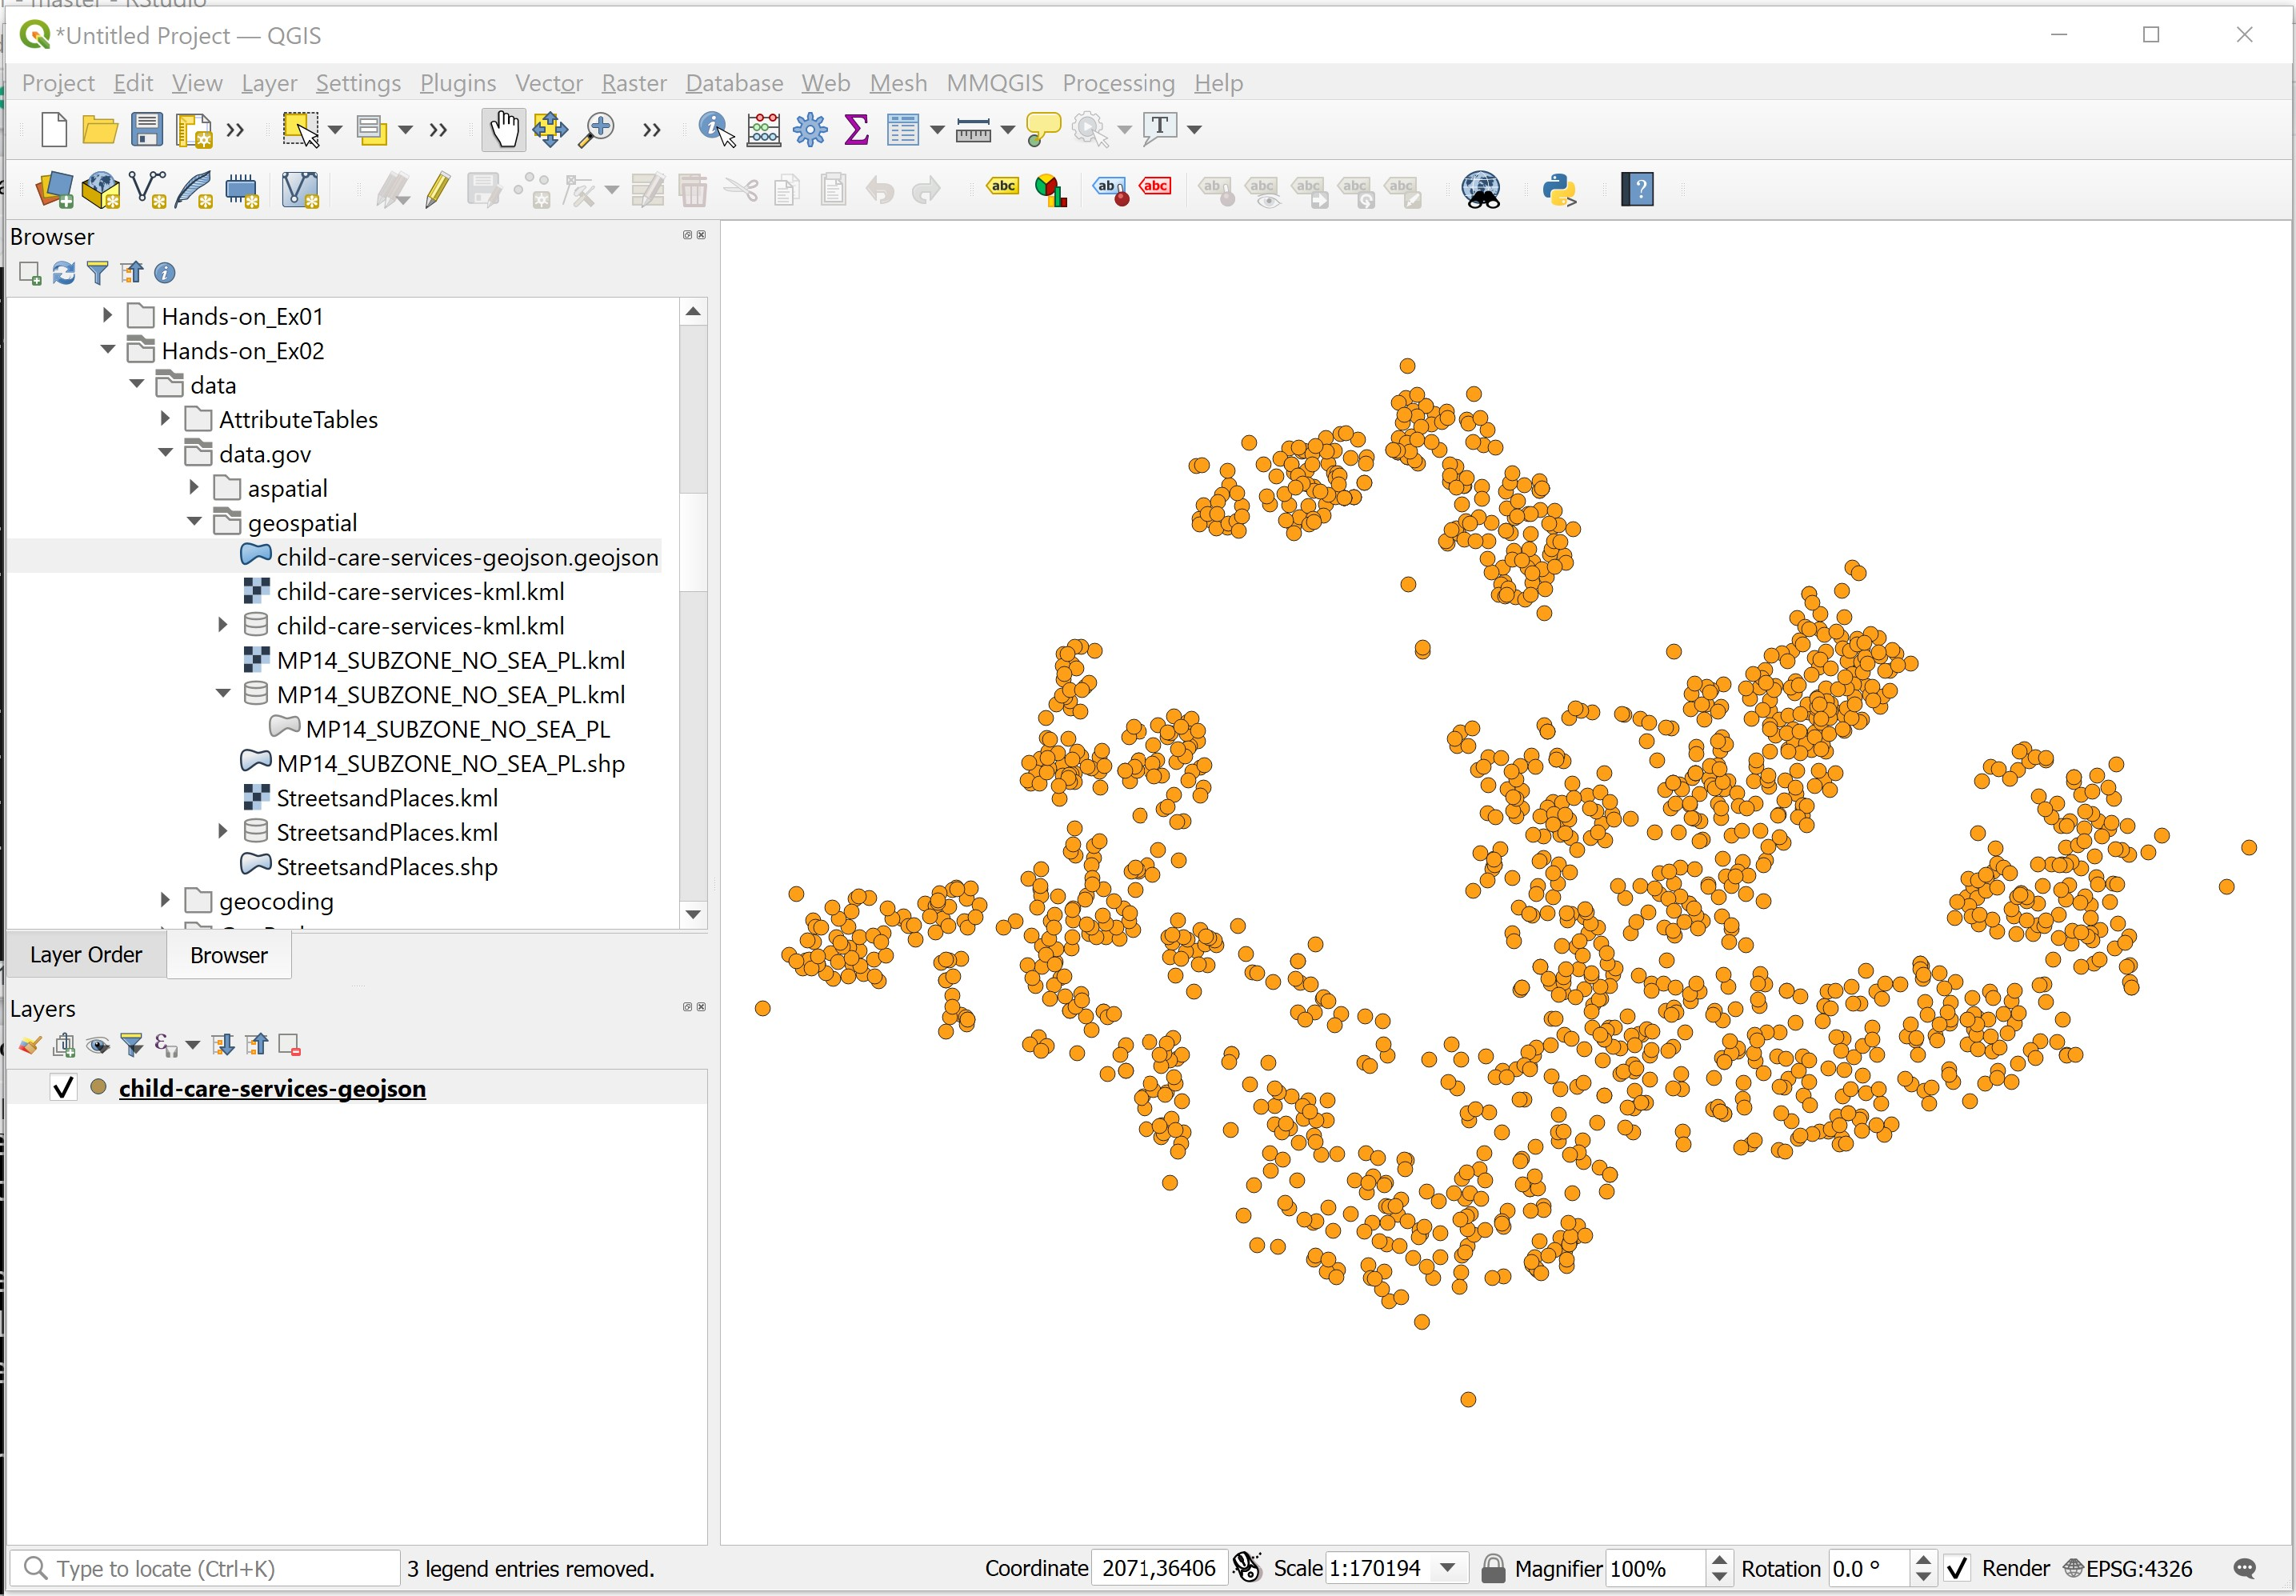
\includegraphics{./img02/image5.jpg}

\begin{quote}
DIY: Using the steps you had learned, bring in
\texttt{MP14\_SUBZONE\_NO\_SEA\_PL.shp} and
\texttt{StreetsandPlaces.shp} into QGIS.
\end{quote}

Your screen should look similar to the figure below.

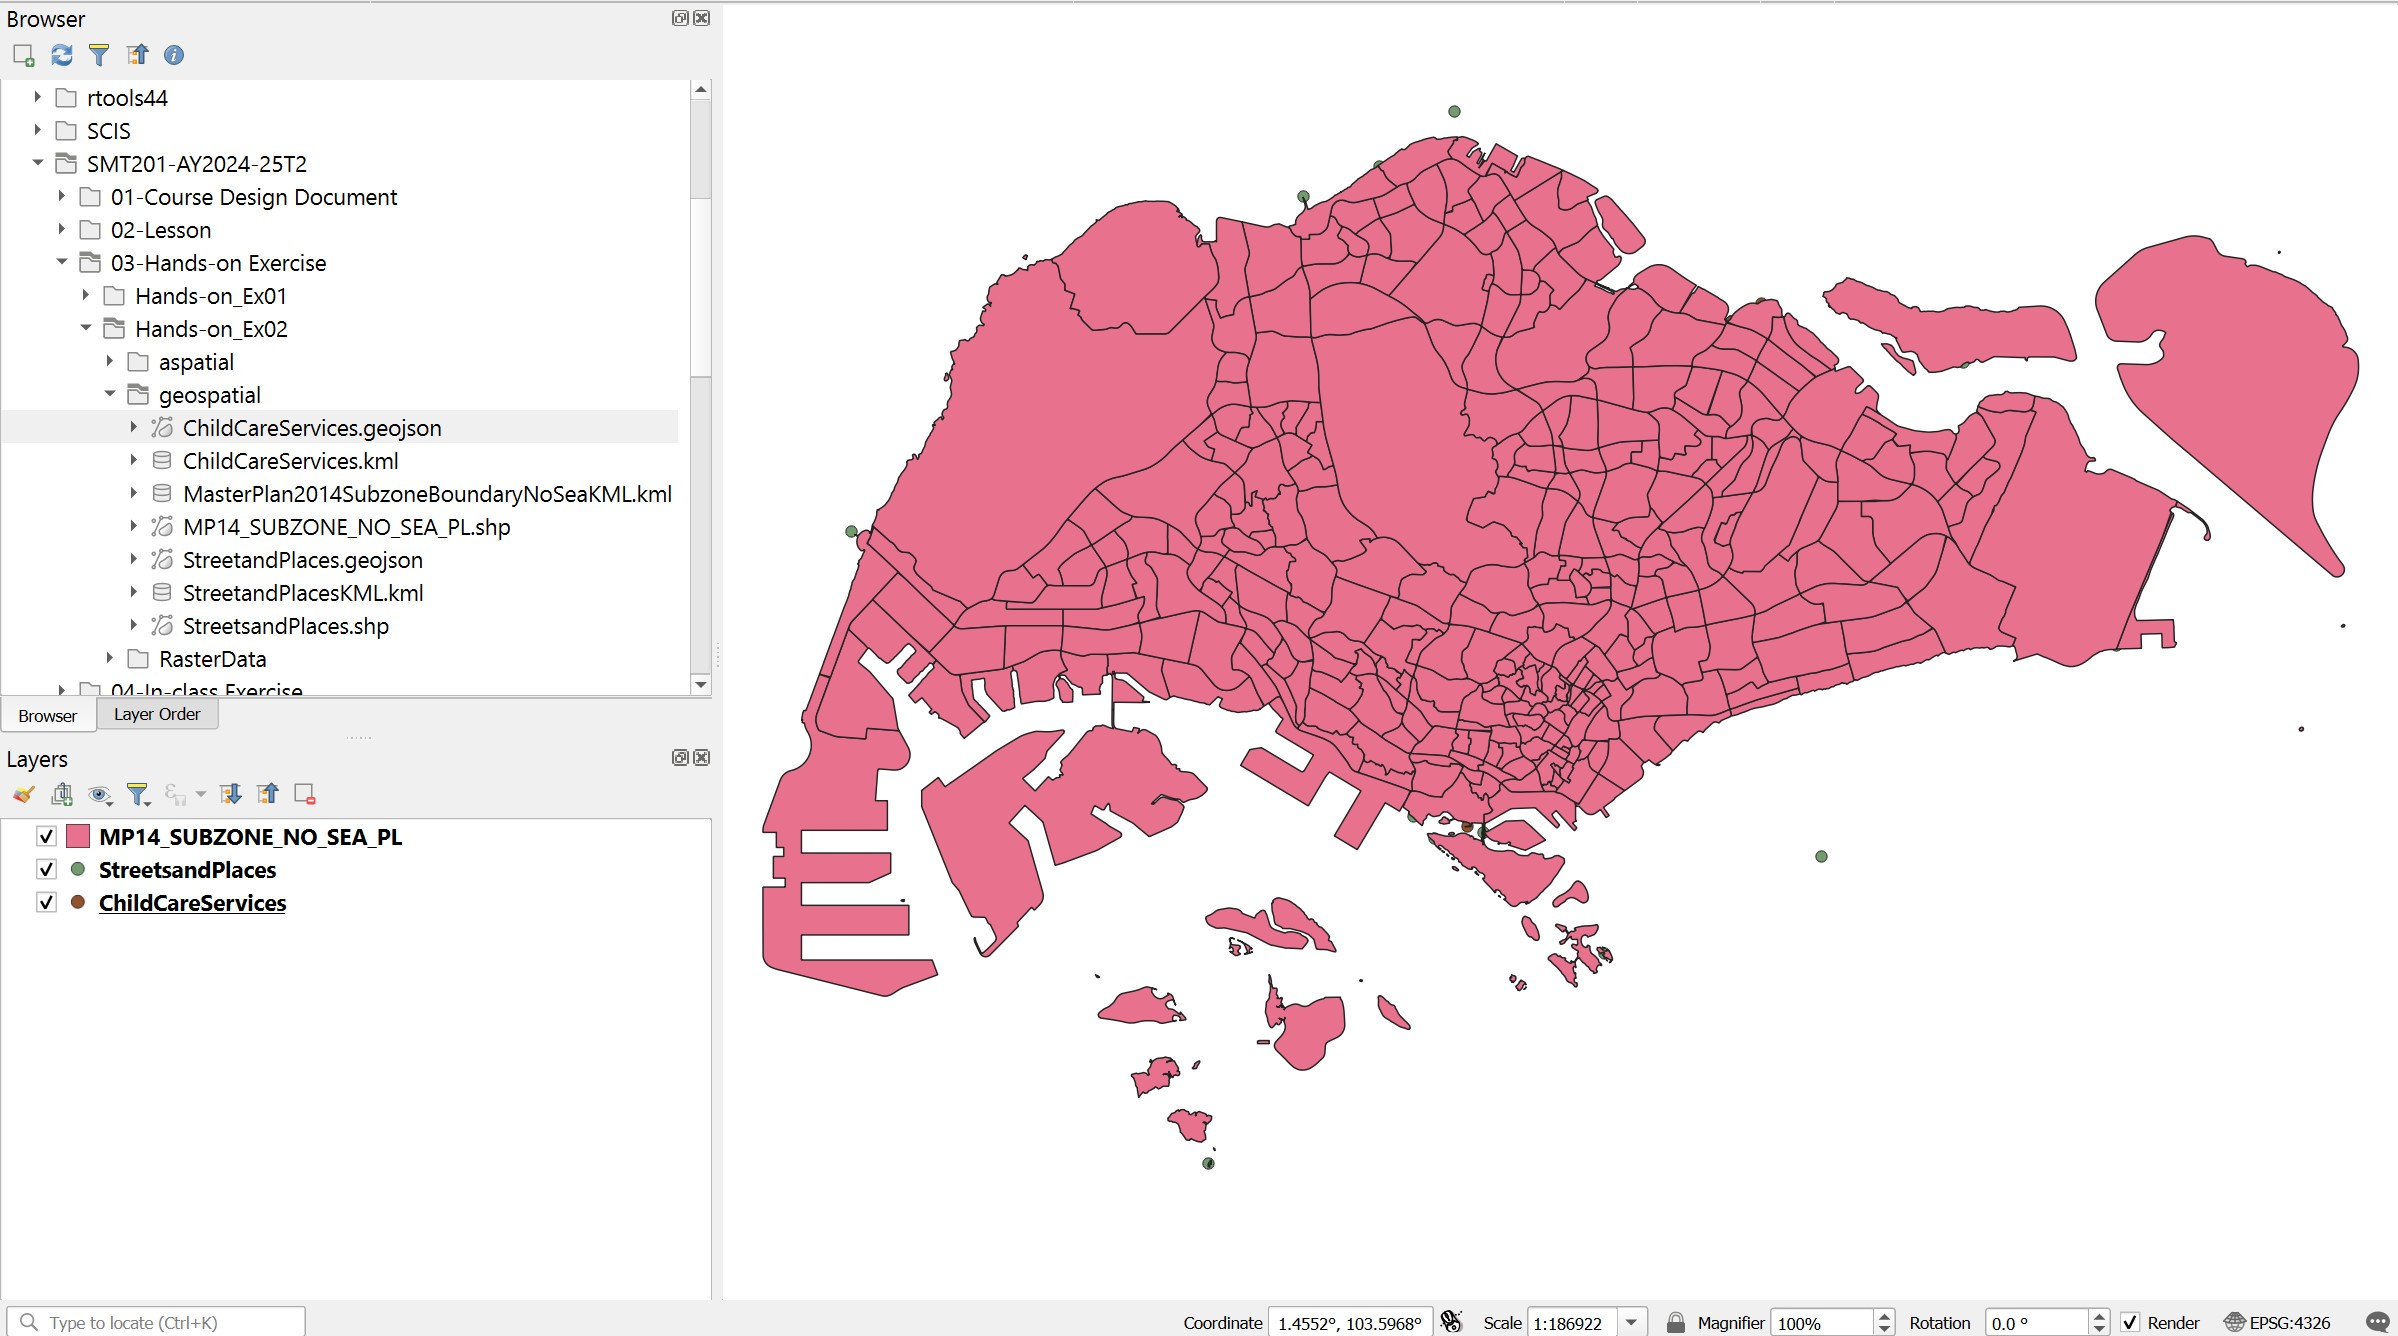
\includegraphics{./img02/image6.jpg}

Notice that \texttt{child-care-services-geojson} layers does not appear
on Map View. This is because it is covered by
\texttt{MP14\_SUBZONE\_NO\_SEA\_PL} layer.

\begin{itemize}
\tightlist
\item
  From the \textbf{Layer} panel, click on
  \texttt{MP14\_SUBZONE\_NO\_SEA\_PL} layer.
\item
  Hold down the left mouse button, drag and place it below
  \texttt{child-care-services-geojson}.
\end{itemize}

Now you should see all the active layers appear on the View window as
shown below.

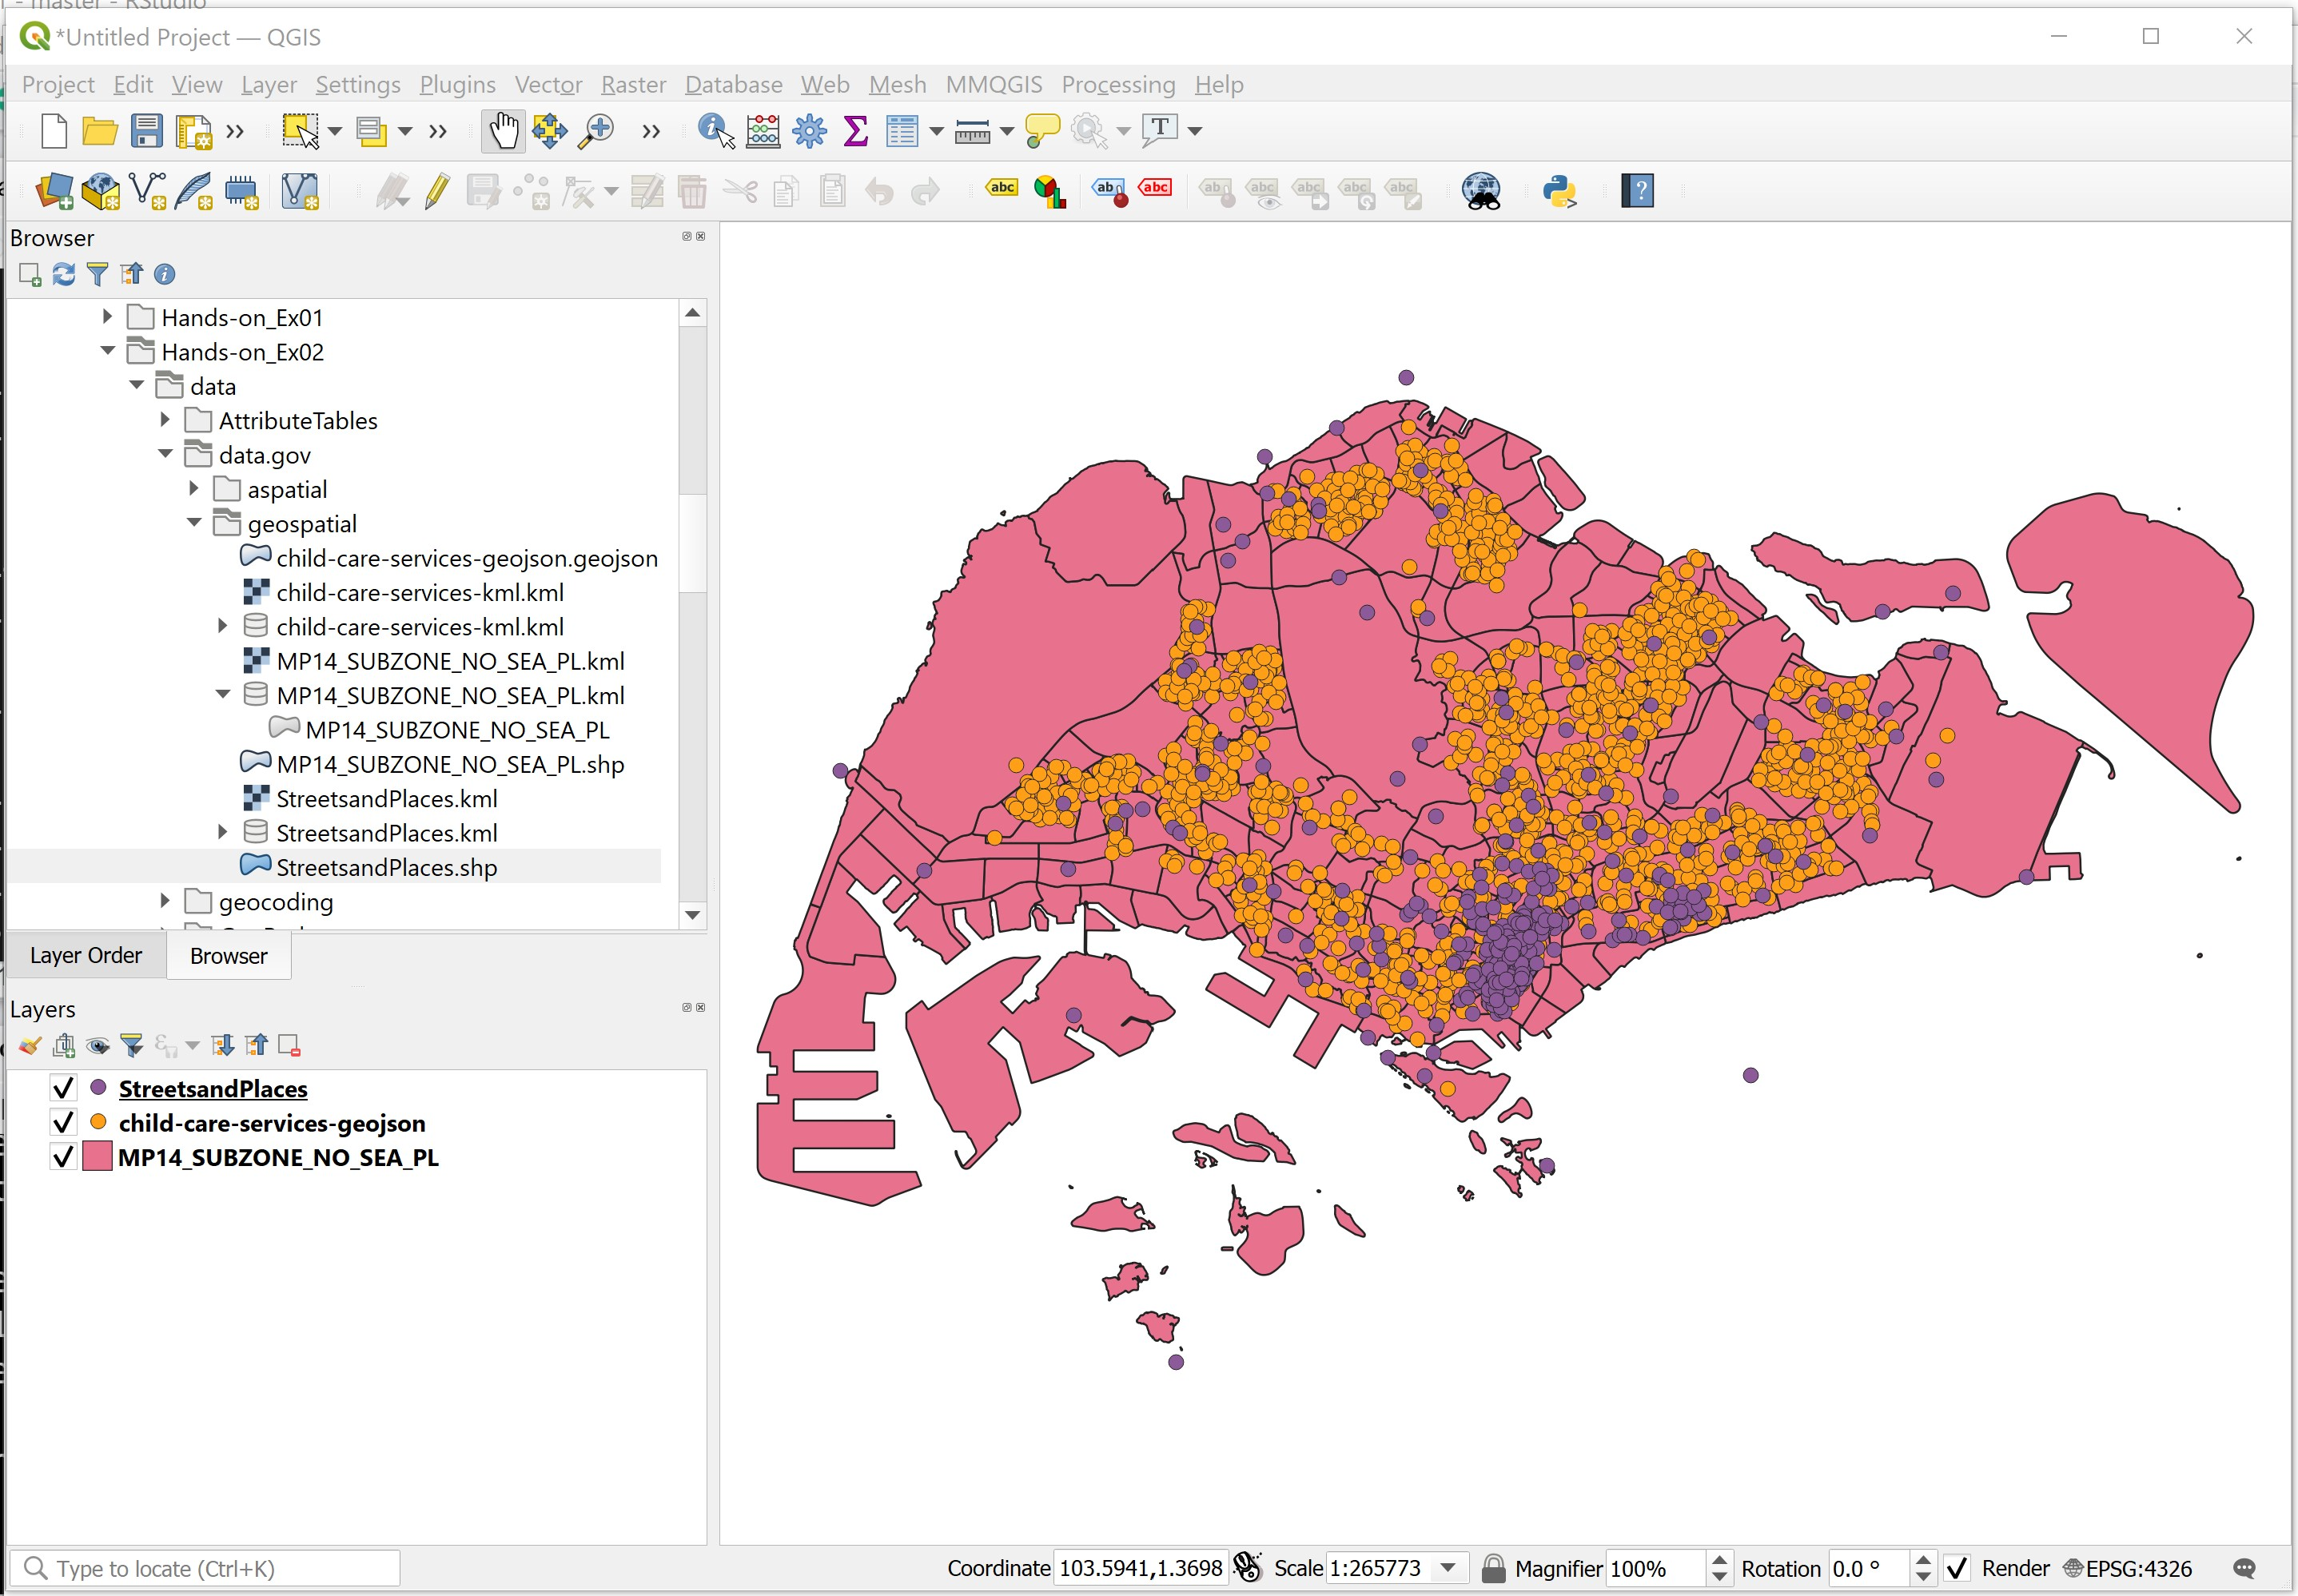
\includegraphics{./img02/image7.jpg}

\begin{quote}
QGIS Tip: In order to avoid point and line feature layers being blocked
away by polygon feature layer, it is always advisible to place the
polygon feature layer at the botton of the layer order.
\end{quote}

It is time to save the project.

\begin{itemize}
\tightlist
\item
  From the menu bar, click \textbf{Project} -\textgreater{}
  \textbf{Save} (Alternatively, from the icon bar, click on \textbf{Save
  Project} icon).
\item
  At the \textbf{Choose a QGIS project file} dialog window, navigate to
  the root project folder, then provide a proper project name such as
  \texttt{Hands-on\_Ex02}, remember to select \emph{QGIS files (}.qgs)*
  from the \textbf{Save as type:} dropdown list.
\end{itemize}

Your screen should look similar to the figure below.

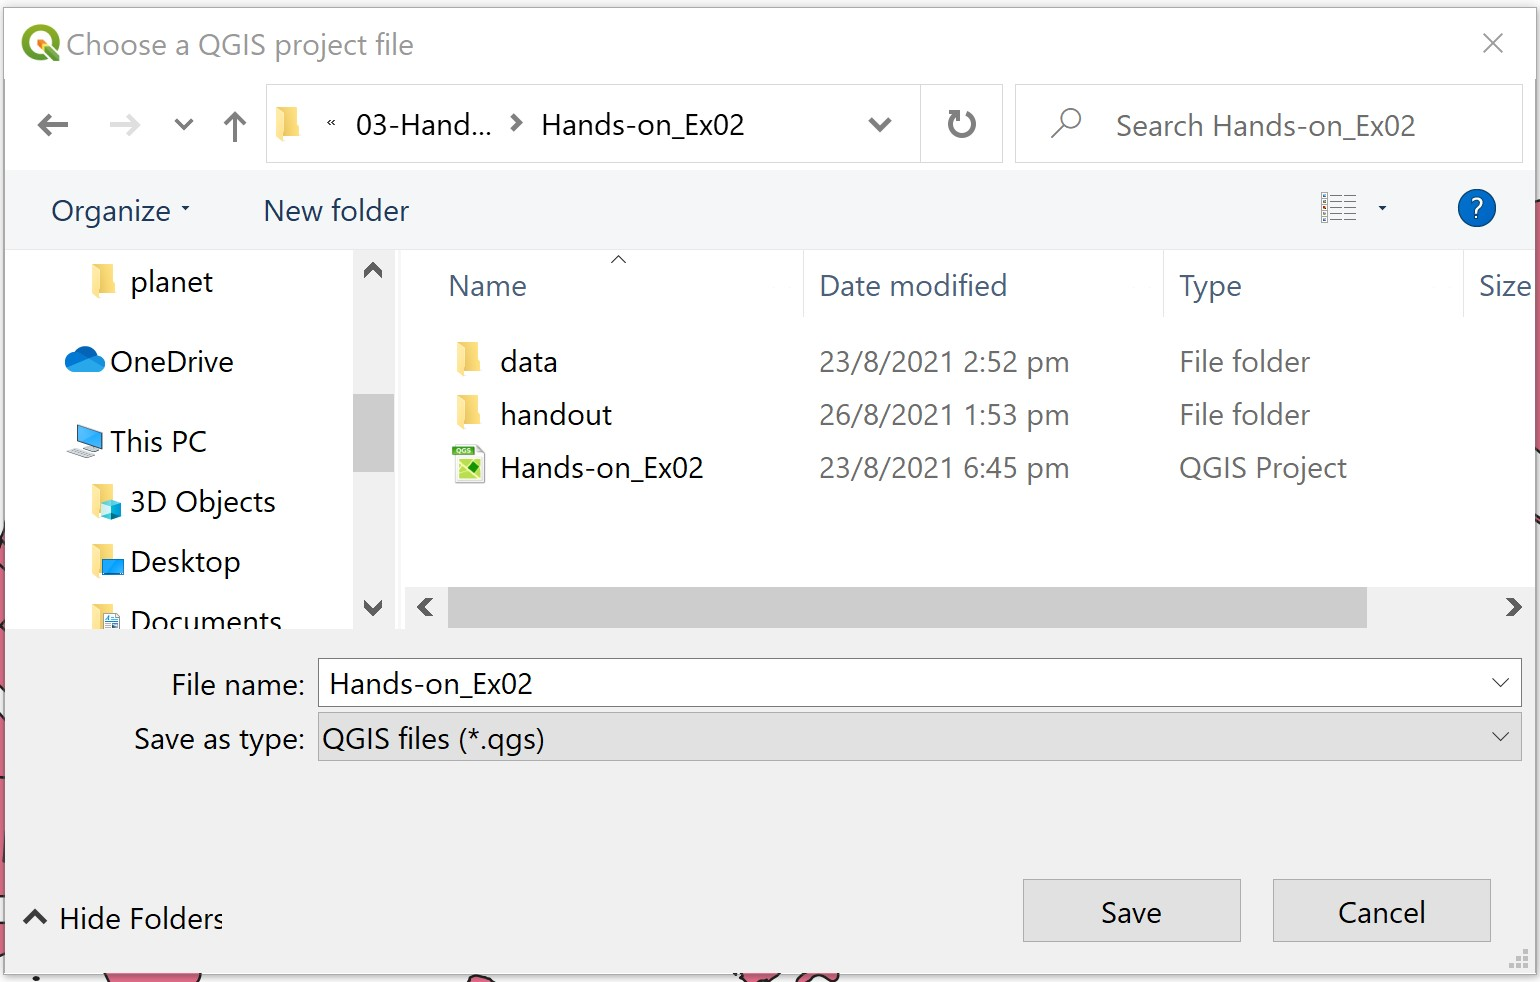
\includegraphics{./img02/image8.jpg}

\begin{itemize}
\tightlist
\item
  click on \textbf{Save} button.
\end{itemize}

Notice that the upper left corner of the top banner is labelled
\texttt{Hands-on\_Ex02} instead of \texttt{untitled} now.

\hypertarget{working-with-projection}{%
\section{Working with Projection}\label{working-with-projection}}

In this section, you will learn how to:

\begin{itemize}
\tightlist
\item
  assign appropriate coordinate system to the QGIS project.
\item
  how to transform a GIS data set from one coordinate system to another
  coordinate system.
\end{itemize}

\hypertarget{assigning-project-coordinate-system}{%
\subsection{Assigning project coordinate
system}\label{assigning-project-coordinate-system}}

If you refer to the lower left corner of the active QGIS project window,
there is a high chance that the EPSG is not in \textbf{3414} which is
the EPSG code of \textbf{svy21}.

If there is the case, you can use the step below to assign the correct
projection system for your QGIS project.

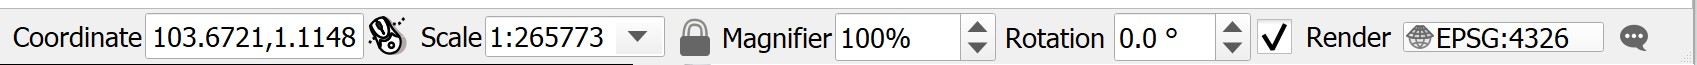
\includegraphics{./img02/image9.jpg}

\begin{itemize}
\tightlist
\item
  At the lower right corner of QGIS project banner, click on the list of
  \textbf{Render}.
\end{itemize}

Project Properties dialog window appears.

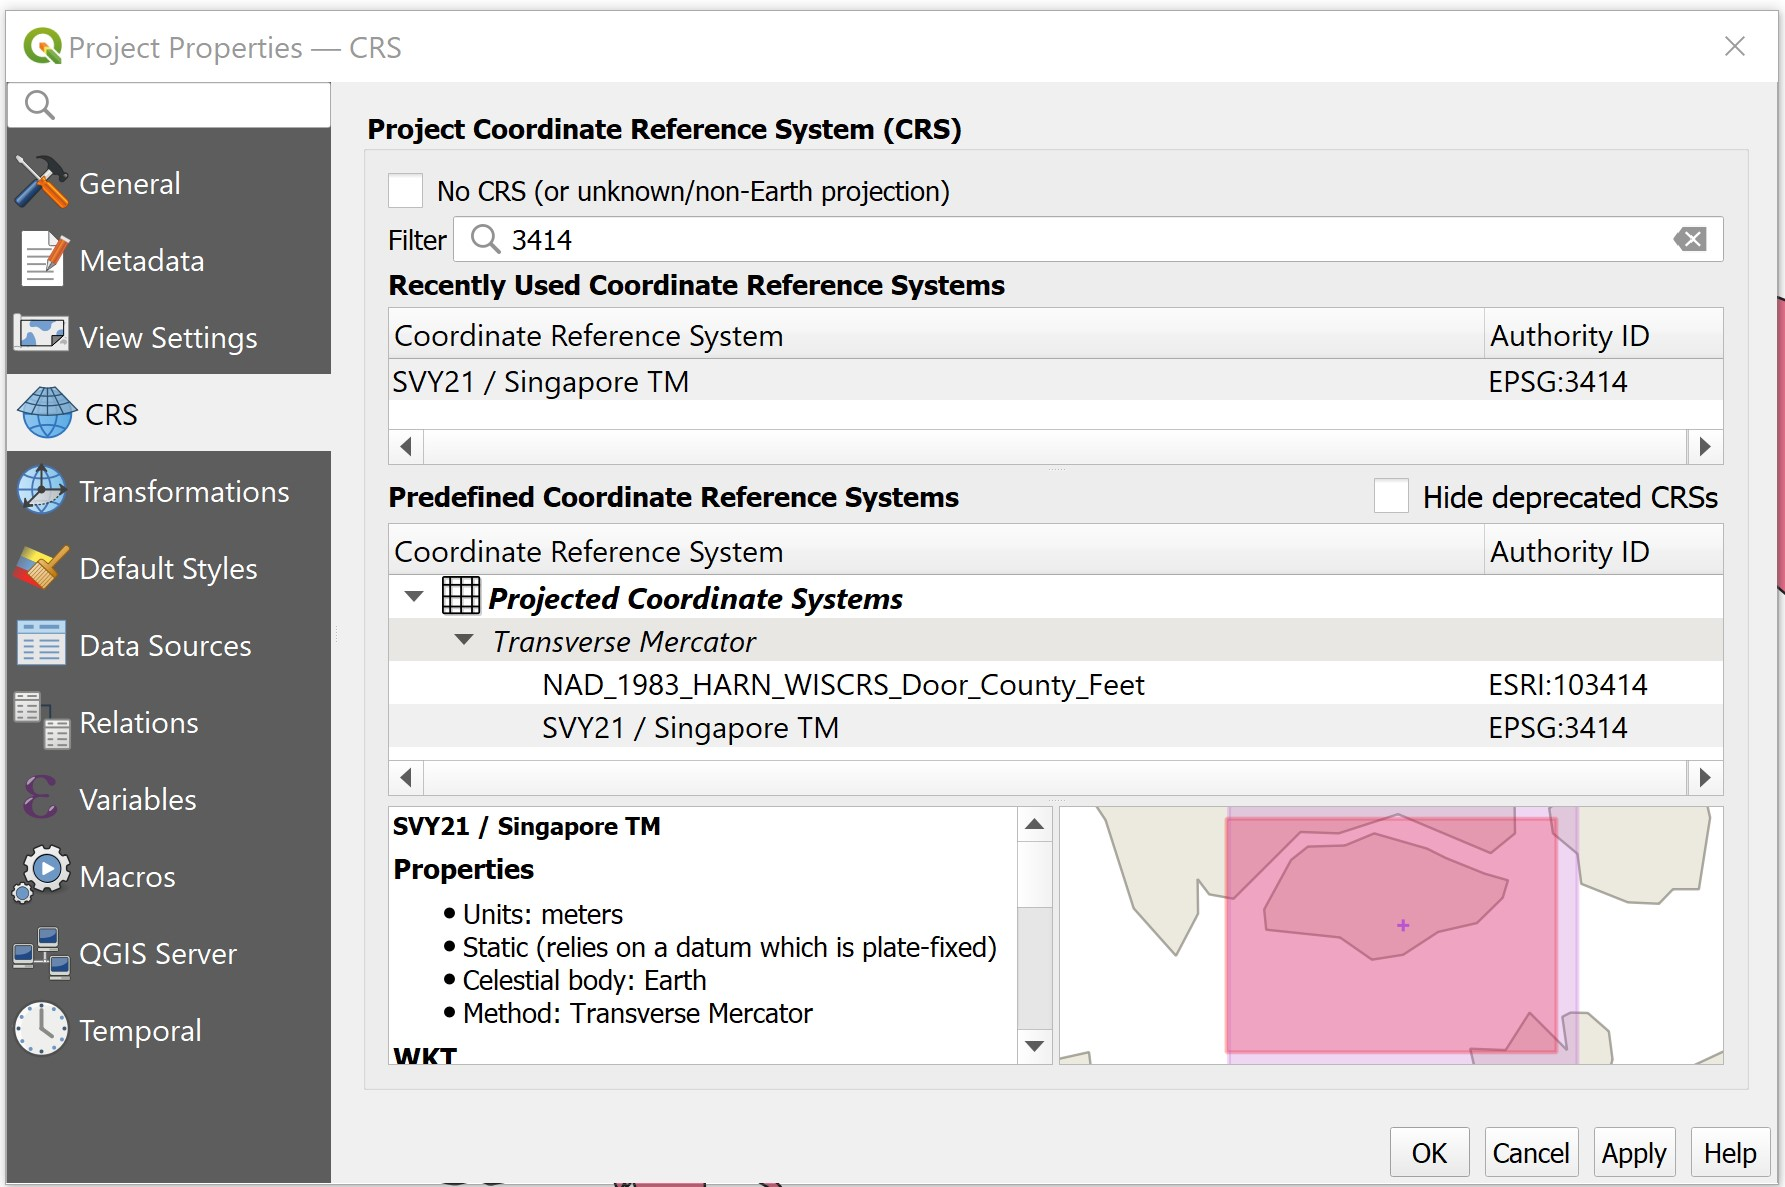
\includegraphics{./img02/image10.jpg}

\begin{itemize}
\tightlist
\item
  From \textbf{Predefined Coordinate Reference Systems}, click on
  \textbf{EPSG:3414} from the list.
\item
  Click on \textbf{Apply} button to make the change.
\item
  Click on \textbf{OK} button to close the window.
\end{itemize}

Notice that the projection has been updated to EPSG:3414 now.

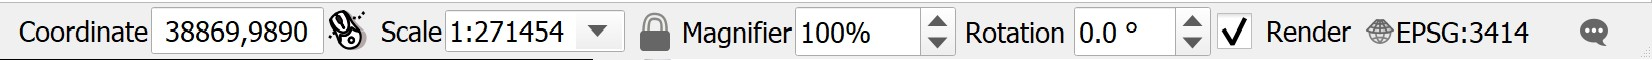
\includegraphics{./img02/image11.jpg}

Option:

If this is the first time you use the \textbf{Projection Properties},
there is a high chance that the \textbf{Predefined Coordinate Reference
Systems} is empty.

In this case,

\begin{itemize}
\tightlist
\item
  at \textbf{Filter}, type \textbf{3414}. This will help to narrow down
  the search.
\end{itemize}

Before you move on to the next section, you should save the latest
changes on the project file.

\begin{itemize}
\tightlist
\item
  From the icon bar, click on the \textbf{Save Project} icon.
\end{itemize}

\hypertarget{transforming-coordinate-system}{%
\subsection{Transforming coordinate
system}\label{transforming-coordinate-system}}

In a GIS project, it is always a good practice to keep the geospatial
data set(s) in a same projected coordinate system, using the national
projected coordinate system such as svy21 of Singapore.

In this section, you will learn how to transform a geospatial data set
from WGS84 Geographic Coordinate System to SVY21 Projected Coordinates
System. You will also learn how to save the output into a new shapefile
for permanent storage purpose. For the purpose of this exercise,
\texttt{child-care-services-geojson} layer will be used.

First, let us verify if an appropriate projection system was used.

\begin{itemize}
\tightlist
\item
  From the \textbf{Layers} panel, right-click on
  \texttt{child-care-services-geojson} layer.
\item
  Select \textbf{Properties}.
\end{itemize}

The Layer Properties dialog window of
\texttt{child-care-services-geojson} layer appears.

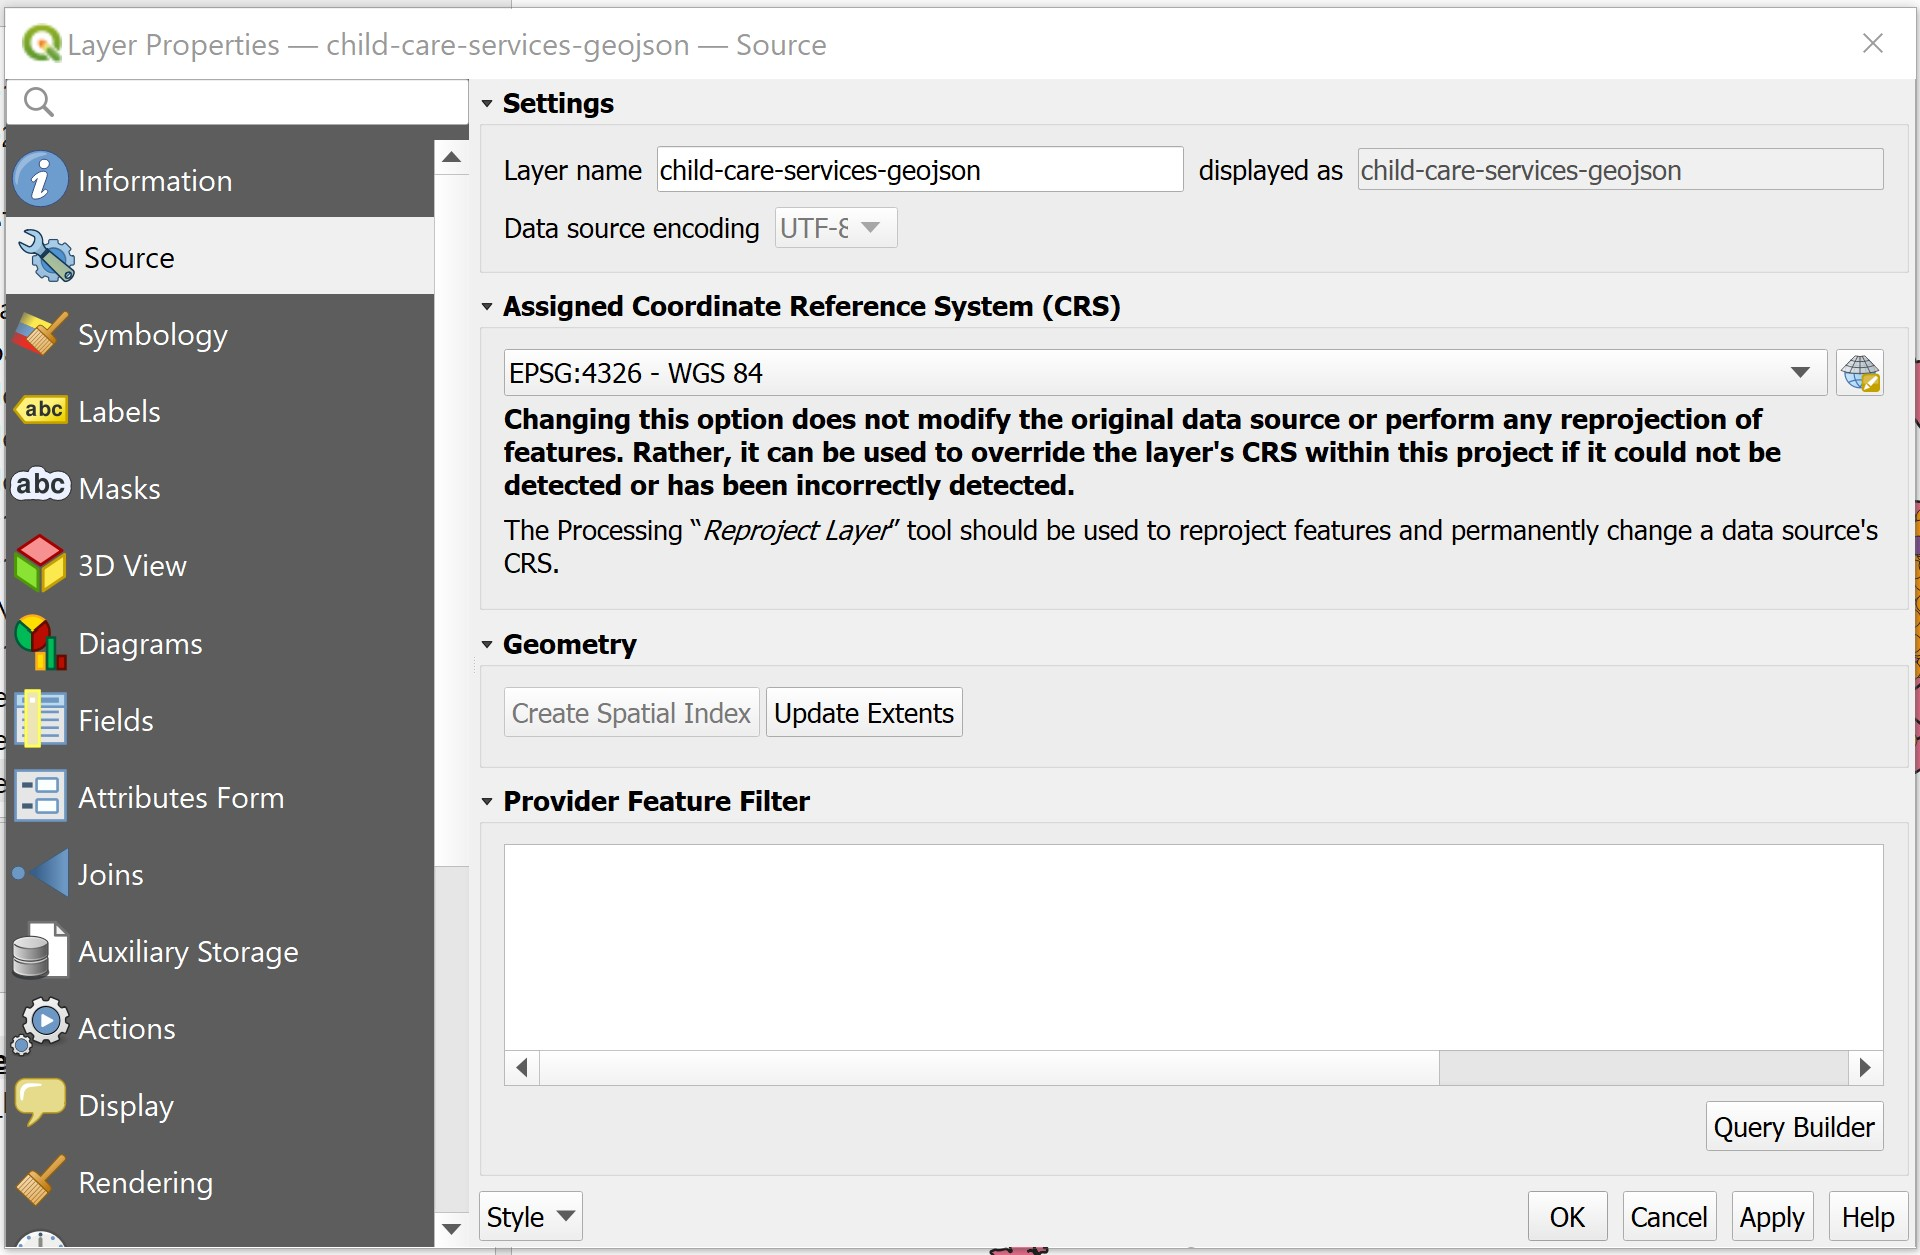
\includegraphics{./img02/image12.jpg}

\begin{itemize}
\tightlist
\item
  Click on \textbf{Source}.
\end{itemize}

Notice that \texttt{child-care-services-geojson} layer is in WGS
geographic coordinates system and not in SVY21 projected coordinates
system.

\begin{itemize}
\tightlist
\item
  Click on \textbf{OK} button to close the dialog window.
\end{itemize}

Next, we are going export the \texttt{child-care-services-geojson} layer
into a new shapefile and at the same time transform the newly created
shapefile into svy21 projected coordinates systems.

\begin{itemize}
\tightlist
\item
  From the \textbf{Layers} panel, right-click on
  \texttt{child-care-services-geojson} layer.
\item
  Select \textbf{Export} -\textgreater{} \textbf{Save Features As} from
  the context menu.
\end{itemize}

The \textbf{Save Vector Layer} dialog window appears.

\begin{itemize}
\tightlist
\item
  For \textbf{Format:}, select ESRI Shapefile from the drop-down list.
\item
  For \textbf{Save as}, click on the \emph{Browse} button.
\end{itemize}

The \textbf{Save Layer As} dialog window appear.

\begin{itemize}
\tightlist
\item
  Navigate to
  \texttt{\textbackslash{}SMT201\textbackslash{}Hands-On02\textbackslash{}data\textbackslash{}data.gov\textbackslash{}geospatial\textbackslash{}}
  sub-folder.
\item
  For File Name, type \texttt{ChildcareServices}.
\end{itemize}

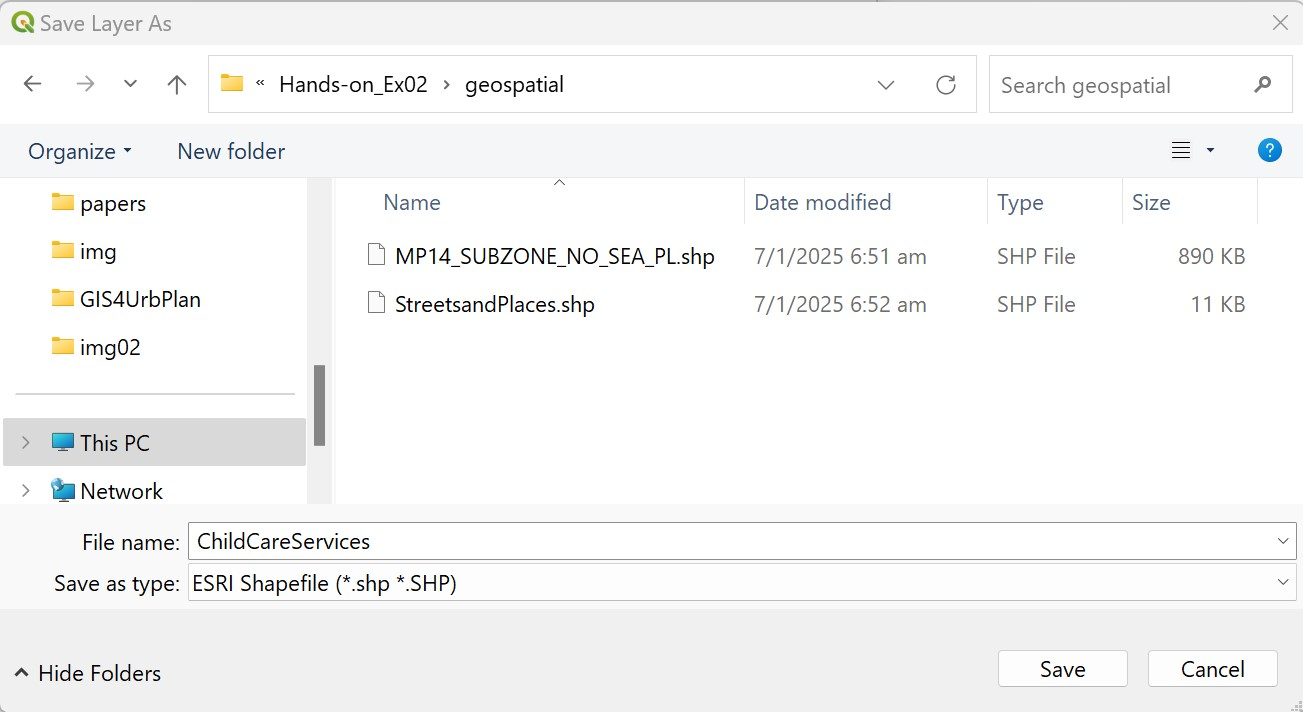
\includegraphics{./img02/image13.jpg}

\begin{itemize}
\tightlist
\item
  Click on the \textbf{Save} button.
\end{itemize}

You will return to \textbf{Save Vector Layer as} dialog window.

Now, you are going to select the appropriate projected coordinate
system.

\begin{itemize}
\tightlist
\item
  For \textbf{CRS}, click on the \textbf{Browse} button.
\end{itemize}

The Coordinate Reference System Selector dialog window appears.

\begin{itemize}
\tightlist
\item
  Click on SVY21/Singapore TM.
\item
  Click on OK to update the selection.
\end{itemize}

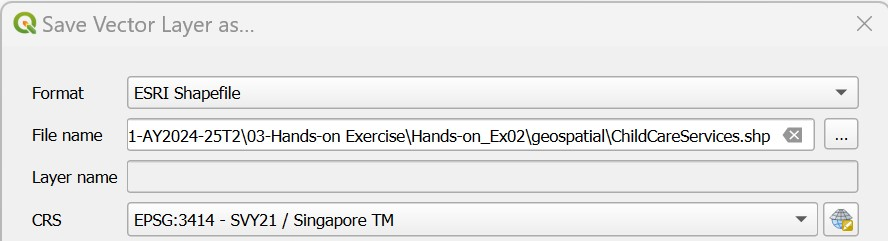
\includegraphics{./img02/image14.jpg}

Notice that the \textbf{CRS} is \textbf{EPSG:3414 - SVY21 / SINGAPORE
TM} now.

Keep the rest of the default option check and you are ready to convert
the geospatial data set into ESRI shapefile format and at the same time
transform it into SVY21 projected coordinate system.

\begin{itemize}
\tightlist
\item
  Click on the OK button.
\end{itemize}

Notice that a new geospatial layer called \texttt{ChildcareServices} has
been added on \texttt{Layers} panel and was plotted on the View window.

\begin{quote}
DIY: Using the steps you had learned in earlier section, check the
properties of of this newly created \texttt{ChildcareServices}
\end{quote}

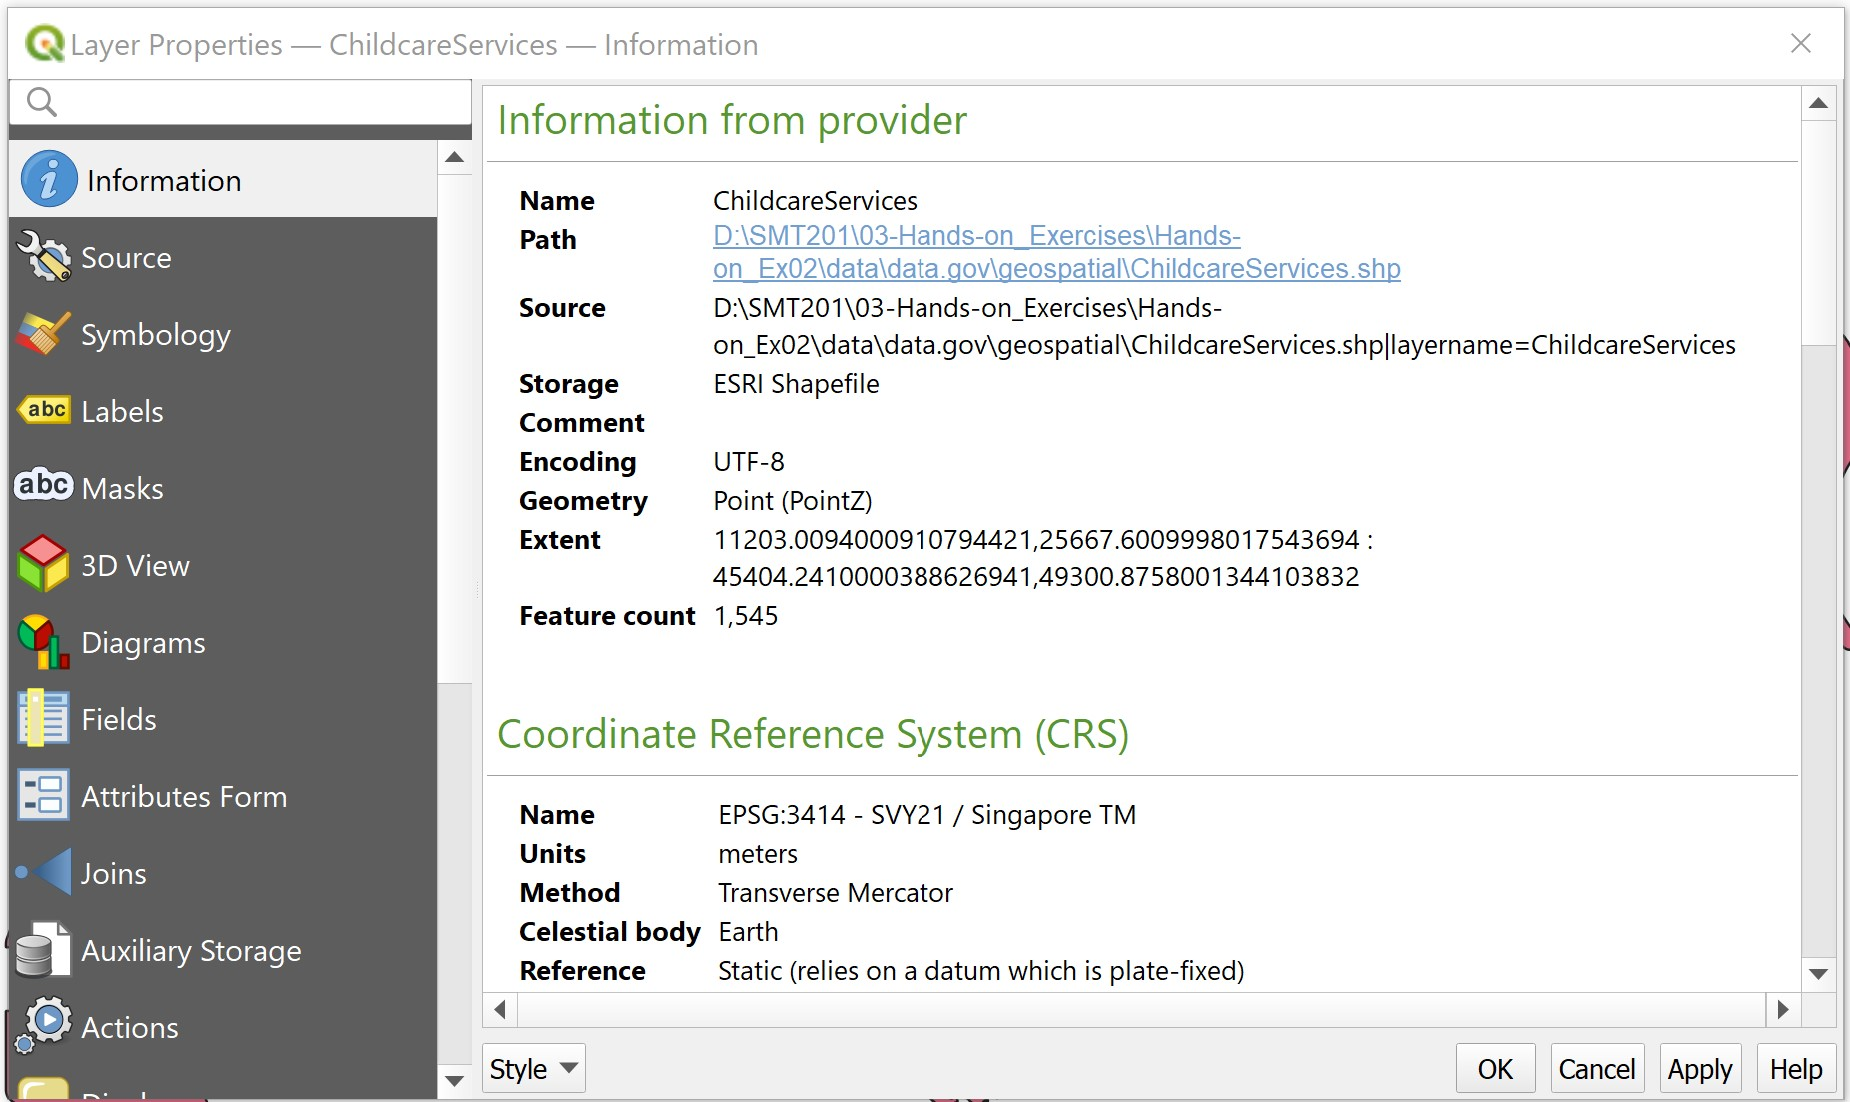
\includegraphics{./img02/image15.jpg}

You screen should look similar to the screensht above.

Notice that \texttt{ChildcareServices} layer is in ESRI Shapefile format
and its Coordinate Reference System in SVY21 / SINGAPORE TM.

\begin{itemize}
\tightlist
\item
  Click on OK button to close the dialog window.
\end{itemize}

\begin{quote}
DIY: You can also remove \texttt{child-care-services-geojson} layer from
Layers dialog window.
\end{quote}

\hypertarget{creating-geospatially-enabled-data}{%
\section{Creating Geospatially-Enabled
Data}\label{creating-geospatially-enabled-data}}

By and large, business data such as polyclinics, schools and business
establishments do not capture geospatial information such as x- and y-
coordinates explicitly. However, it is possible to create
geospatially-enabled data from them by using the geocoding technique.

Geocoding is the process of finding associated geographic coordinates
(often expressed as latitude and longitude) from other geographic data,
such as street addresses, zip codes or postal codes
(http://en.wikipedia.org/wiki/Geocoding).

\hypertarget{data-preparation}{%
\subsection{Data Preparation}\label{data-preparation}}

In this section, you will learn how to create geospatially enable data
by using \texttt{general-information-of-schools.csv} you downloaded from
data.gov.sg.

Note: In this section, we assume that
\texttt{general-information-of-schools.csv} is stored in
\texttt{\textbackslash{}Hands-on\_Ex02\textbackslash{}data\textbackslash{}data.gov\textbackslash{}aspatial\textbackslash{}}
sub-folder and you have Microsoft Excel installed in your computer.

Let us review the content of \texttt{general-information-of-schools.csv}
file.

\begin{itemize}
\tightlist
\item
  At File Explorer, navigate to the sub-folder where
  \texttt{general-information-of-schools.csv} is stored.
\item
  Right-click on \texttt{general-information-of-schools.csv} file.
\item
  From the context menu, select \textbf{Open with} -\textgreater{}
  \textbf{Excel}.
\end{itemize}

Your screen should look similar to the figure below.

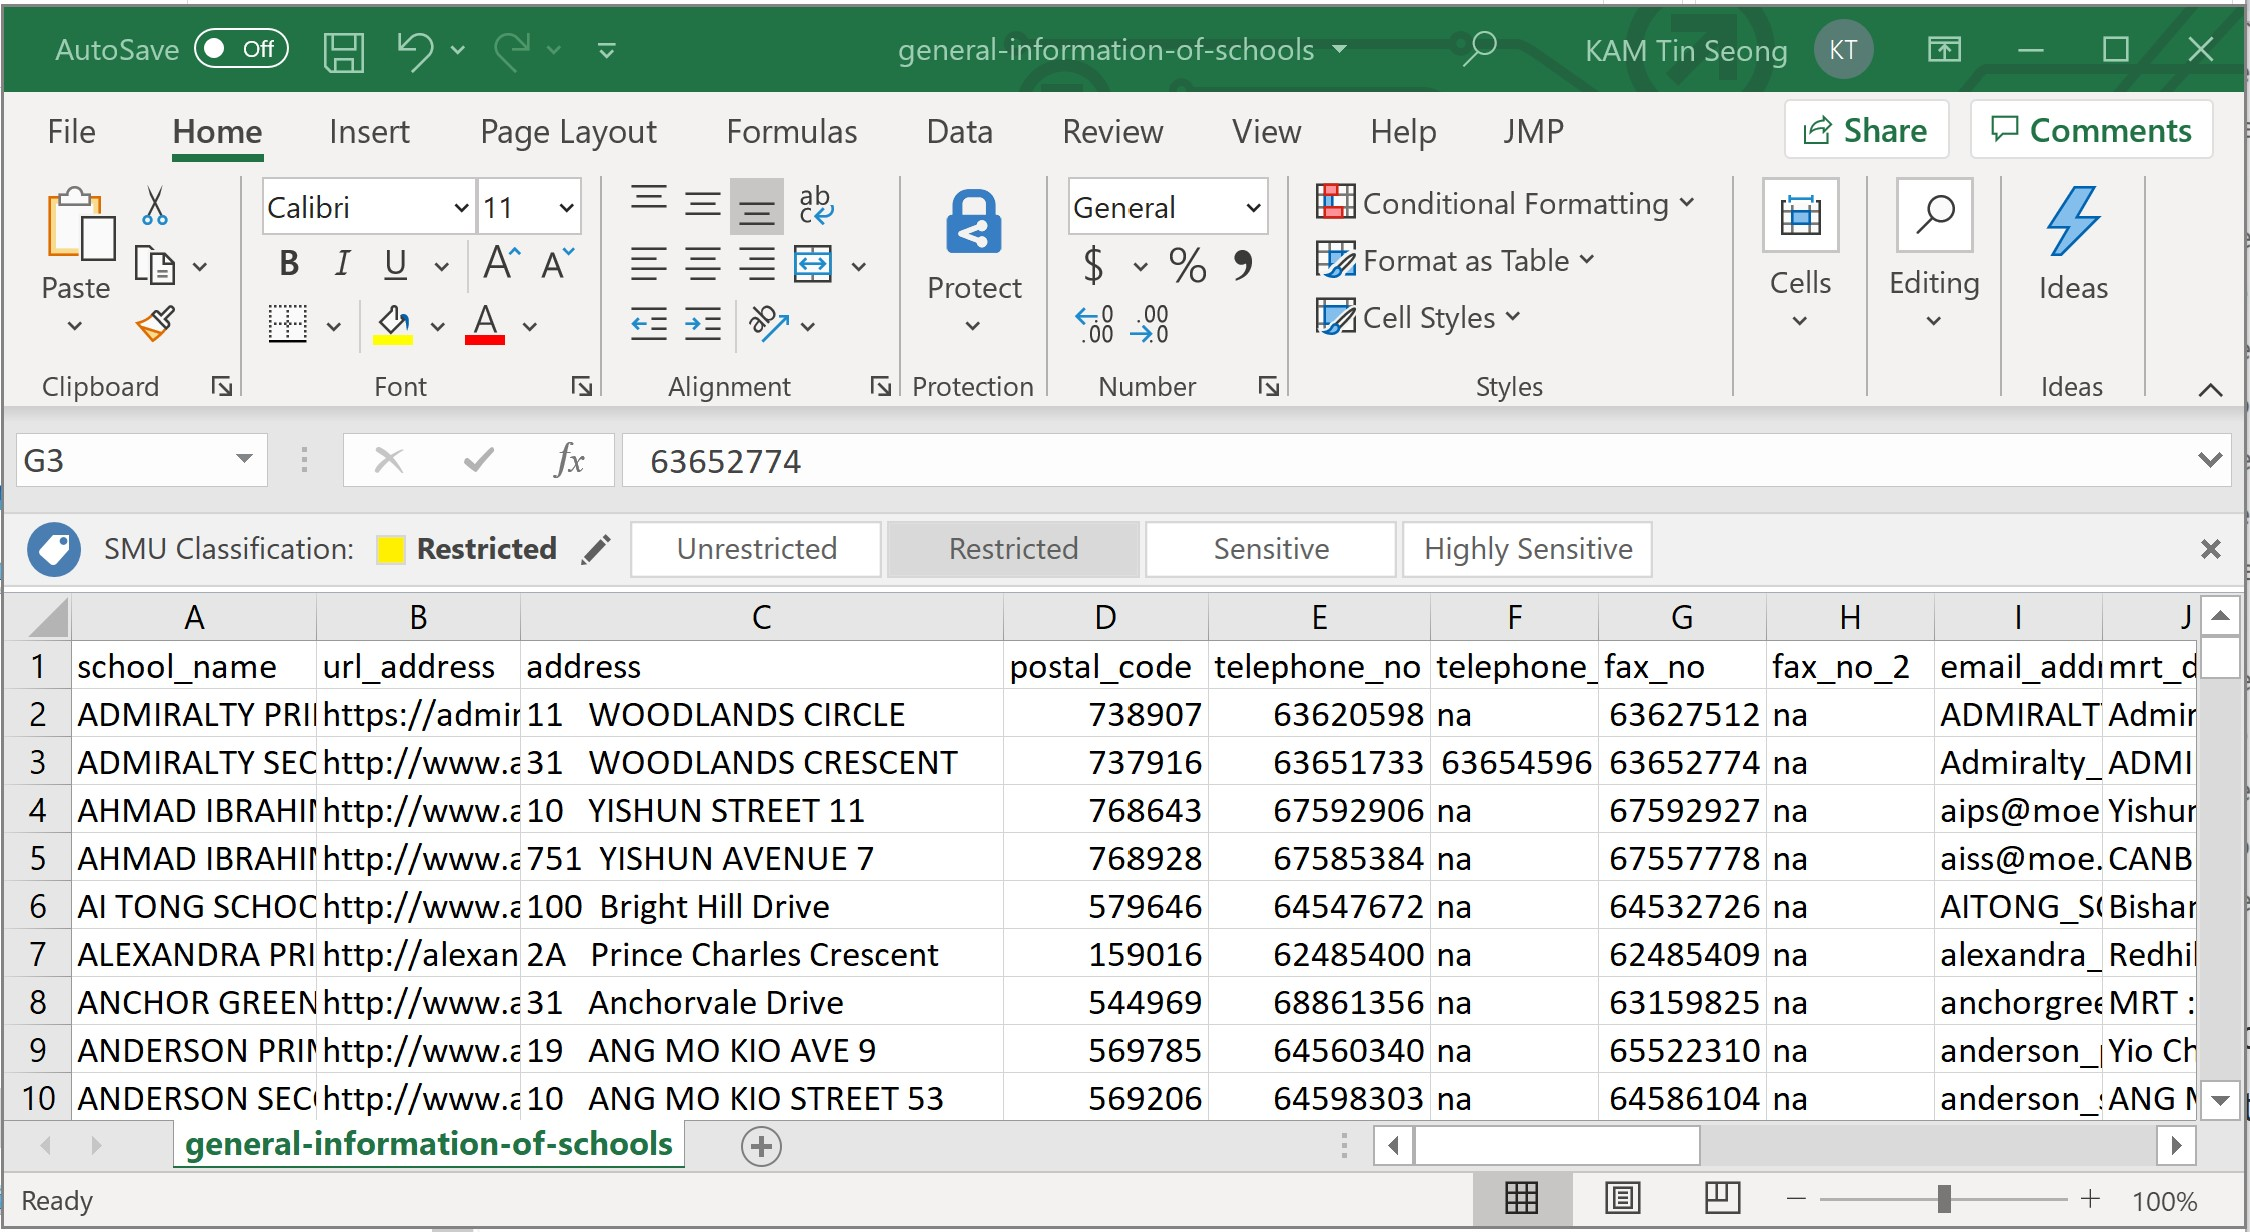
\includegraphics{./img02/image16.jpg}

Notice that \texttt{general-information-of-schools.csv} file consists of
31 fields. However, we only need to retain \texttt{school\_name},
\texttt{address} and \texttt{postal\_code} field.

\begin{itemize}
\tightlist
\item
  Use appropriate Excel function to delete the unwanted fields.
\end{itemize}

Next, we will create two create two new fields. They are:
\texttt{country} and \texttt{city}.

\begin{itemize}
\tightlist
\item
  Use appropriate Excel function to create two new fields. Call them
  \texttt{country} and \texttt{city}.
\item
  Fill in the cell below \texttt{country} and \texttt{city} fields with
  \texttt{Singapore}.
\end{itemize}

The final \texttt{general-information-of-schools.csv} should look
similar to the screenshot below.

\includegraphics{./img02/image17.jpg}

\begin{itemize}
\tightlist
\item
  Use the \emph{Save as} function of Excel to save the tidied csv file
  into Hands-on\_Ex02\data\data.gov\aspatial sub-folder. Name the output
  file \texttt{schools.csv}.
\end{itemize}

\begin{quote}
Note: It is important to ensure that the output file is in csv file
format.
\end{quote}

\hypertarget{install-the-mmqgis-plugin}{%
\subsection{Install the MMQGIS Plugin}\label{install-the-mmqgis-plugin}}

Instead of using the geocoding API of SLA OneMap, in this section you
will use the \emph{Geocode Tools} of
\href{http://michaelminn.com/linux/mmqgis/}{\textbf{MMQGIS}} plugin
developed by Michael Minn.

To install the \textbf{MMQGIS} plugin, you will need to load the QGIS
plugin repository by following the steps below.

\begin{itemize}
\tightlist
\item
  From the menu bar, select \textbf{Plugins} --\textgreater{}
  \textbf{Manage and Install Plugins}.
\end{itemize}

Plugins dialog window appears as shown below.

\includegraphics{./img02/image18.jpg}

Notice that there is a long list of plugins available. We can use the
Search function to locate mmqgis plugin easily.

\begin{itemize}
\tightlist
\item
  At Search, type \emph{mmqgis}.
\end{itemize}

Your screen should look similar to the figure below.

\includegraphics{./img02/image19.jpg}

\begin{quote}
\textbf{Friendly Advice:} It is a good practice to read the
documentation of the plugin (i.e.~More info: homepage) thoroughly before
download or/and using any QGIS plugin.
\end{quote}

\begin{itemize}
\tightlist
\item
  Click on \textbf{Install Plugin} button to run the installer.
\end{itemize}

After installing mmqgis plugin, remember to close the Plugin dialog
window.

\begin{itemize}
\tightlist
\item
  Click on \textbf{Close} button.
\end{itemize}

\hypertarget{geocoding-using-mmqgis-plugin}{%
\subsection{Geocoding using MMQGIS
Plugin}\label{geocoding-using-mmqgis-plugin}}

Now, you are ready geocode \texttt{schools} dataset.

\begin{itemize}
\tightlist
\item
  From the menu bar, select \textbf{MMQGIS} -\textgreater{}
  \textbf{Geocode} -\textgreater{} \textbf{Geocode CSV with Web
  Service}.
\end{itemize}

Web Service Geocode dialog window appears.

\includegraphics{./img02/image20.jpg}

Geocode Tools of MMQGIS plugin imports addresses from a CSV file. The
input CSV file should be encoded in the UTF-8 character set. Although
other 8-bit encodings (like Windoze ISO-8859-x) will work if only ASCII
characters are present, non-ASCII characters may cause unpredictable
behavior.

\begin{itemize}
\tightlist
\item
  From \textbf{Input CSV File (UTF-8)}, click on \textbf{Browse} button.
\end{itemize}

\textbf{Select a file} dialog window appears.

\begin{itemize}
\tightlist
\item
  Navigate to the path where \texttt{schools.csv} reside.
\item
  Click on \texttt{schools.csv}.
\item
  Click on \textbf{Open} button.
\end{itemize}

Your screen should similar to the screenshot below.

\includegraphics{./img02/image21.jpg}

Notice that the \textbf{Address}, \textbf{City} and \textbf{Country}
drop-down lists have been mapped to the corresponding field names in
\texttt{schools.csv}. This explains why the data preparation performed
in previous step was important and necessary.

\textbf{MMQGIS Geocode Tool} supports five geocoding services. They are:
Google, OpenStreetMap/Nomination, US Census Bureau, ESRI Server and
NetToolKit. Except OpenStreetMap/Nomination, the rest of the geocoding
services required you to have an API key.

In this exercise, OpenStreetmap/Nominatim geocoding service will be
used.

\begin{quote}
Warning: To complete this section, you will need internet access to run
the geocoding process.
\end{quote}

\begin{itemize}
\tightlist
\item
  For \emph{Web Service}, select \textbf{OpenStreetMap/Nominatim} from
  the drop-down list.
\end{itemize}

Geocode Tool will generate two output files. They are a point feature
GIS data set along with a \emph{Not Found CSV} file containing all rows
that could not be geocoded (for whatever reason). We need to tell
Geocode Tool where to keep these two output files.

\begin{itemize}
\tightlist
\item
  Use File Explorer to create a new sub-folder called geocoding in
  \Hands-on\_Ex02\data~directory.
\item
  For \textbf{Output File Name}, click on \textbf{Browse} button.
\end{itemize}

\textbf{Create or select a file} dialog window appears.

\begin{itemize}
\tightlist
\item
  Navigate to the newly create \emph{geocoding} sub-folder.
\item
  For \textbf{File name}, type \texttt{geocoded\_sch.shp}.
\item
  Click on \textbf{Save} button.
\end{itemize}

You also need to provide the \textbf{Not Found List Output list} a place
holder.

\begin{itemize}
\tightlist
\item
  For \textbf{Not Found Output list}, click on \textbf{Browse} button.
\end{itemize}

\textbf{Create or select a file} dialog window appears.

\begin{itemize}
\tightlist
\item
  Navigate to the newly create \emph{geocoding} sub-folder.
\item
  For \textbf{File name}, type \texttt{not\_found\_sch.csv}.
\item
  Click on \textbf{Save} button.
\end{itemize}

The completed dialog window should look similar to the screenshot below.

\includegraphics{./img02/image22.jpg}

Now, you are ready to perform the geocoding function.

• At the \textbf{Web Service Geocode} dialog window, click on
\textbf{Apply} button.

When the geocoding function is completed, notice that a new shapefile
layer will be added on QGIS map window. At the same time, the progress
bar will indicate numbers of records that have been geocoded
successfully as shown below.

\includegraphics{./img02/image23.jpg}

The output report shows that out of the 346 schools data records, 325 of
them have been geocoded successfully.

\begin{itemize}
\tightlist
\item
  click on \textbf{Close} button to closed the dialog window.
\end{itemize}

Let us examine the layer properties of the newly created
\texttt{geocoded\_sch} layer.

\begin{itemize}
\tightlist
\item
  Hover your mouse over geocoded\_sch layer, right-click and select
  \textbf{Open Attribute Table} from the context menu.
\end{itemize}

The \textbf{Attribute tabl}e of \texttt{geocoded\_sch} appears.

\includegraphics{./img02/image24.jpg}

Notice that all columns from the input CSV file are added as attributes
in the output shapefile. Six additional fields are added to in the
shapefile. The \textbf{category} and \textbf{type} fields are internal
from OpenStreetMap. They provide useful data classification for the
schools data sets.

\begin{quote}
DIY: Using the steps your had learned in previous section, examine and
transform the coordinate system of \texttt{geocoded\_sch} data set into
SVY21 projected coordinate system.
\end{quote}

\hypertarget{working-with-raster-gis-data}{%
\section{Working with Raster GIS
data}\label{working-with-raster-gis-data}}

Raster data such as those collected by remote sensing satellite or
airplanes are one of the important data sources of a GIS project. By and
large, these data are stored in image file format such as TIF, GeoTIF,
JPG and GeoJPG. In this section, you will learn how to bring a raster
data in GeoTIF file format into QGIS. The raster data is called
Chinatown.tif. It is available in
\Hands-on\_Ex02\data\RasterData sub-folder.

\begin{itemize}
\tightlist
\item
  Start \textbf{File Explorer}.
\item
  Navigate to \Hands-on\_Ex02\data\RasterData sub-folder.
\end{itemize}

You should see the following files in the sub-folders.

\includegraphics{./img02/image25.jpg}

This is an example of images file in GeoTIF format. The geographical
information of the image file (i.e.~Chinatown.TIF) is actually contained
in the Chinatown.XML file.

\begin{itemize}
\tightlist
\item
  Open \texttt{Chinatown.XML} using \textbf{Notepad}.
\end{itemize}

It should look similar to the figure below.

\includegraphics{./img02/image26.jpg}

It provides details information of the image file including georeference
system used, the geographical extent of the data, spectral resolution of
the dataset and spatial resolution of the dataset.

Next, you will important Chinatown raster data into QGIS.

\begin{itemize}
\tightlist
\item
  From \textbf{Browser} panel, navigate to sub-folder as shown in the
  screenshot below.
\end{itemize}

\includegraphics{./img02/image27.jpg}

\begin{itemize}
\tightlist
\item
  Double-click on \texttt{Chinatown.tif}.
\end{itemize}

Notice that a new raster layer called Chinatown has been added on the
\textbf{Layers} panel. However, it is not visible on the View window.
This is because it is block by the massive point features.

In order to view the newly added \texttt{Chinatown} layer, we need to
zoom into the extend of \texttt{Chinatown} layer.

\begin{quote}
DIY: Using the steps you had learned in Hands-on Exercise 1, zoom to the
extend of \texttt{Chinatown} layer.
\end{quote}

Your screen should look similar to the screenshot below.

\includegraphics{./img02/image28.jpg}

\begin{quote}
DIY: Using the steps you had learn in the earlier sections of this
hands-on exercise, examine the properties of \texttt{Chinatown} data
layer.
\end{quote}

\hypertarget{working-with-internet-geospatial-services}{%
\section{Working with Internet Geospatial
Services}\label{working-with-internet-geospatial-services}}

One of the unique feathers of a modern GIS is its capability of
consuming GIS data shared over the internet. These data can be in the
form of WMS, WMS or proprietary format such as Google map, Bing map and
OpenStreetMap format. In this section, you will learn how to consume an
OpenStreetMap (OSM) data using QGIS.

DIY: Before we can use OSM service, let us display the map view by using
the full extent of \texttt{MP14\_SUBZONE\_NO\_SEA\_PL} layer. This is
because we will use the extend of \texttt{MP14\_SUBZONE\_NO\_SEA\_PL} as
the reference to map OSM service in QGIS.

\begin{itemize}
\tightlist
\item
  From \textbf{Browser} panel, click on the triangle in front of
  \textbf{XYZ Tiles}.
\end{itemize}

OpenStreetMap icon appears as shown in the screenshot below.

\includegraphics{./img02/image29.jpg}

\begin{itemize}
\tightlist
\item
  Double-click on \textbf{OpenStreetMap} icon.
\end{itemize}

Your screen should look similar to the figure below.

\includegraphics{./img02/image30.jpg}

\begin{quote}
DIY: Use the skills you had learned from previous sections, 1.
Re-organise the GIS layers so that you can see the polyclinics, and
childcare centres are plotted on top of OpenStreetMap layer. 2. Navigate
around the map areas and look for details.
\end{quote}

\bookmarksetup{startatroot}

\hypertarget{gis-mapping-and-geovisualisation}{%
\chapter{GIS Mapping and
Geovisualisation}\label{gis-mapping-and-geovisualisation}}

In this exercise, you will learn how to prepare qualitative and
quantitative thematic maps using QGIS. You will also learn how to create
a joint table by using the concept of georelational data model of GIS.

\hypertarget{learning-outcome-1}{%
\section{Learning Outcome}\label{learning-outcome-1}}

By the end of this session, you will be able to:

\begin{itemize}
\tightlist
\item
  prepare qualitative maps,
\item
  create proportional symbol map,
\item
  perform georelational join,
\item
  Compute new field from existing fields, and
\item
  prepare choropleth map.
\end{itemize}

\hypertarget{data}{%
\section{Data}\label{data}}

For the purpose of this hands-on exercise, three data sets are provided.
They are:

\begin{itemize}
\tightlist
\item
  \texttt{education} provides general information of public primary
  schools, secondary schools and junior colleges. This data set was
  downloaded from Data.gov.sg and geocoded by using SLA OneMap Api.
\item
  \texttt{sgpools} provides information of SG Pools outlets and stores
  information.
\item
  \texttt{POP2020} provides population by age group as at June 2020. It
  is downloaded from Department of Statistics (DOS), Singapore. The data
  set provides multiple years of population data. For the purpose of
  this exercise, only 2020 data were extracted.
\end{itemize}

These three data sets are in csv file format. They can be found in
\texttt{DataTables} of Hand-on\_Ex03 folder.

Besides the above three data sets, you are required to download the
following geospatial from public web sites:

\begin{itemize}
\tightlist
\item
  \texttt{National\ Map\ Polygon} from Data.gov.sg
\item
  \texttt{Master\ Plan\ 2014\ Subzone\ Boundary\ (No\ Sea)} from
  Data.gov.sg
\item
  \texttt{Road\ Section\ Line} from LTA Data Mall
\end{itemize}

\hypertarget{data-preparation-1}{%
\subsection{Data Preparation}\label{data-preparation-1}}

\begin{quote}
DIY: Using the steps you had learned from the previous hands-on
exercise, convert the education and SGPools data sets in DataTables
folder into geospatial data layer and store them into an integrated
database called \texttt{SG}. The geospatial database must be in
\textbf{GeoPackage} format.
\end{quote}

\begin{quote}
DIY: Using the steps you had learned from the previous hands-on
exercise, convert the geospatial data sets downloaded from Data.gov.sg
and LTA Data Mall into the newly created \texttt{SG} database.
\end{quote}

\hypertarget{getting-started-1}{%
\section{Getting Started}\label{getting-started-1}}

\begin{quote}
DIY: Launch QGIS. Create a new project call \texttt{Hands-on\_Ex03}.
Provide the project with a correct referencing system.
\end{quote}

\begin{quote}
DIY: Using the steps you had learned from the previous hands-on
exercies, import all the geospatial data in \texttt{SG} database into
the newly created QGIS project.
\end{quote}

\begin{quote}
DIY: Using the steps you had learned from the previous hands-on
exercise, add OSM map layer into \texttt{Hands-on\_Ex03} project.
\end{quote}

Your screen should look similar to the figure below.

\includegraphics{./img03/image1.jpg}

\hypertarget{symbolising-qualitative-gis-data-layers}{%
\section{Symbolising Qualitative GIS Data
Layers}\label{symbolising-qualitative-gis-data-layers}}

In this section, you will learn how to symbolise GIS data layers by
using their corresponding qualitative data values.

\hypertarget{symbolising-education-gis-layer}{%
\subsection{Symbolising education GIS
layer}\label{symbolising-education-gis-layer}}

The \texttt{type\_code} field of \texttt{Education} layer provides us
the school type information. In this section, you will learn how to use
this field to symbolise \texttt{education} layer.

\begin{itemize}
\tightlist
\item
  At \textbf{Layers} panel, click on \texttt{Education} layer to make it
  active.
\item
  Right-click on \texttt{Education} and select \textbf{Properties} from
  the context menu.
\end{itemize}

The \textbf{Layer Properties} dialog window appears.

\begin{itemize}
\tightlist
\item
  Click on the \textbf{Symbology} tab.
\end{itemize}

Your screen should look similar to the screenshot below.

\includegraphics{./img03/image2.jpg}

\begin{itemize}
\tightlist
\item
  Select \textbf{Categorized} from the \textbf{Symbol drop-down} list.
\end{itemize}

\includegraphics{./img03/image3.jpg}

\begin{itemize}
\tightlist
\item
  For \textbf{Value}, select \emph{mainlevel\_code} from the drop-down
  list.
\end{itemize}

\includegraphics{./img03/image4.jpg}

\begin{itemize}
\tightlist
\item
  Click on the \textbf{Classify} button.
\end{itemize}

Your screen should look similar to the screenshot below.

\includegraphics{./img03/image5.jpg}

Figure above shows that \texttt{Education} layer has been categorised
into five categories. They are, Junior College, Centralised Institute,
Mixed Levels, Primary and Secondary.

Next, you will learn how to symbolise them by using the svg vector
symbol set.

\begin{itemize}
\tightlist
\item
  Double-click on the marker in front of \emph{JUNIOR COLLEGE}.
\end{itemize}

The \textbf{Symbol selector} dialog window appears.

\includegraphics{./img03/image6.jpg}

\begin{itemize}
\item
  From \textbf{Marker}, click on \textbf{Simple marker}.
\item
  For \textbf{Symbol layer type}, select \textbf{SVG maker} from the
  drop-down list.
\end{itemize}

Scroll down the dialog window until you can see the SVG Browser as shown
below.

\includegraphics{./img03/image7.jpg}

\begin{itemize}
\tightlist
\item
  From the \textbf{SVG Image}, scroll-down and click on
  \includegraphics{./img03/image8.jpg}.
\end{itemize}

\begin{quote}
DIY: Change the size value and fill colour and observe the differences.
\end{quote}

\begin{itemize}
\tightlist
\item
  When you are done, click on the \textbf{OK} button.
\end{itemize}

You will return to \textbf{Layer Properties} dialog window.

\begin{quote}
DIY: Using the step you had learned, change the symbols of the remaining
four categories in \emph{mainlevel\_code} field.
\end{quote}

When you are done.

\begin{itemize}
\tightlist
\item
  At the \textbf{Layer Properties} dialog window, click on
  \textbf{Apply} button to update the changes.
\item
  To close the \textbf{Layer Properties} dialog window, click on OK
  button.
\end{itemize}

Your screen should look similar to the figure below.

\includegraphics{./img03/image9.jpg}

This map is popularly known as Point symbol map among the GIS and
cartography communities. Prior to GIS era, this kind of map took more
than a month to prepare. With GIS, it only needs less than 15 minutes to
prepare. The advantage of GIS-based point symbol map is that the map can
be changed easily with very little effort. GIS-based point symbol map is
also highly interactive. You can navigate around the digital map and
zoom in to view the distribution in greater details.

\begin{quote}
DIY: Use the steps you had learned from the previous section, symbolise
the
\end{quote}

\begin{quote}
Challenge: Using the steps you had learned in the previous section,
symbolise RoadSectionLine layer according to Expressway and Roads.
\end{quote}

\begin{quote}
Challenge: Using the steps you had learned in the previous section,
symbolise National Map Polygon layer to show the outlines only.
\end{quote}

Your screen should look similar to the figure below.

\includegraphics{./img03/image10.jpg}

\hypertarget{creating-proportional-symbol-map}{%
\section{Creating Proportional Symbol
Map}\label{creating-proportional-symbol-map}}

\textbf{Proportional symbol} maps (also known as graduate symbol maps)
are a class of maps that use the visual variable of size to represent
differences in the magnitude of a discrete, abruptly changing
phenomenon, e.g.~counts of people. Like choropleth maps, you can create
classed or unclassed versions of these maps. The classed ones are known
as \textbf{range-graded} or \textbf{graduated symbols}, and the
unclassed are called \textbf{proportional symbols}, where the area of
the symbols are proportional to the values of the attribute being
mapped.

In this section, you will learn how to create a proportional symbol map
showing the numbers of win by Singapore Pools' outlets.

\begin{quote}
DIY: Before we get started, let us switch off \texttt{Education},
\texttt{RoadSectionLine} and \texttt{SGOutline} layers.
\end{quote}

Your screen should look similar to the figure below.

\includegraphics{./img03/image11.jpg}

Before you start to prepare the proportional symbol map, you will take a
look at the attribute table of \texttt{SGPools} layer.

\begin{itemize}
\tightlist
\item
  At the \textbf{Layers} panel, right-click on \texttt{SGPools} layer.
\item
  Select \textbf{Open Attribute Table} from the context menu.
\end{itemize}

Your screen should look similar to the figure below.

\includegraphics{./img03/image12.jpg}

You are going to use the values in the last filed (e.g
\emph{Gp1Gp2Winn}) to create a proportional symbol map.

\begin{itemize}
\tightlist
\item
  Close the table by clicking on the cross icon located at the upper
  right corner of the table.
\end{itemize}

Next, you are going to change the size of the point symbol by mapping
the values in \emph{Gp1Gp2Winn} field.

\begin{itemize}
\tightlist
\item
  At the \textbf{Layers} panel, right-click on \textbf{SGPools} layer.
\item
  Select \textbf{Properties} from the context menu.
\end{itemize}

The \textbf{Layer Properties} dialog window appears.

\begin{itemize}
\item
  Click on the \textbf{Symbology} icon.
\item
  For \textbf{Value}, select \emph{Gp1Gp2Winngs} from the dropdown list.
\item
  For \textbf{Method}, select \textbf{Size} from the drop-down list.
\item
  For \textbf{Size} to, type \emph{10}.
\item
  Click on \textbf{Classify} button.
\end{itemize}

Your screen should look similar to the figure below.

\includegraphics{./img03/image13.jpg}

When you are ready,

\begin{itemize}
\tightlist
\item
  Click on \textbf{Apply} button to update the changes.
\end{itemize}

In order to view the changes, you need to close the dialog window.

\begin{itemize}
\tightlist
\item
  Click on \textbf{OK} to close the \textbf{Layer Properties} dialog
  window.
\end{itemize}

Your screen should look similar to the figure below.

\includegraphics{./img03/image14.jpg}

Notice that there are many proportional symbols were overlapping. Now,
you will learn how to use the layer transparent feature of QGIS to
improve the visualisation.

\begin{quote}
DIY: Using the step you had learned in the earlier section, open the
\textbf{Layer Properties} of \texttt{SGPools}.
\end{quote}

\begin{itemize}
\tightlist
\item
  At the \textbf{Layer Properties} panel, look for \textbf{Layer
  rendering} sub-panel located at the bottom ot the dialog window.
\item
  Click on the little triangle in front of \textbf{Layer rendering}
  sub-panel.
\end{itemize}

The Layer rendering subpanel extended as shown in the figure below.

\includegraphics{./img03/image15.jpg}

\begin{itemize}
\tightlist
\item
  For \textbf{Opacity}, type \emph{80\%}, alternatively, you can use
  slider to slide toward the left until it reaches 80\%.
\end{itemize}

To update the changes,

\begin{itemize}
\tightlist
\item
  Click on \textbf{Apply} button.
\end{itemize}

Lastly,

\begin{itemize}
\tightlist
\item
  Click on \textbf{OK} button to close the dialog window.
\end{itemize}

Your screen should look similar to the figure below.

\includegraphics{./img03/image16.jpg}

• Feel free to explore other configurations. When you are done, click on
the \textbf{OK} button.

\hypertarget{choropleth-map-using-gis}{%
\section{Choropleth map using GIS}\label{choropleth-map-using-gis}}

\textbf{Choropleth mapping} involves the symbolisation of enumeration
units, such as countries, provinces, states, counties or census units,
using area patterns or graduated colors. For example, a social scientist
may need to use a choropleth map to portray the spatial distribution of
aged population of Singapore by Master Plan 2014 Subzone Boundary.

The major concerns of choropleth mapping are the method of data
classification, areal symbolization, and the overall map design. General
rules for choropleth mapping are as follows:

\begin{itemize}
\tightlist
\item
  Use data that are assumed to be uniform throughout an enumeration
  unit.
\item
  Because enumeration units vary in size, do not map totals. Use derived
  values, such as ratios, rates, proportions, or percentages.
\item
  The best classing method depends on the data, the map reader and the
  purpose of the map.
\item
  When classifying data, the full range of data must be included and
  class values should not overlap. No more than six classes are
  recommended.
\item
  Class symbols (i.e.~colors or patterns) must be easily
  distinguishable.
\end{itemize}

In this section of the hands-on exercise, you will learn how to use QGIS
to prepare a choropleth map showing the distribution of population with
age 65 and above in Singapore by URA's Master Plan 2014 subzone. You
will also gain hands-on experience on the various data classification
methods, symbolisation and map layout design techniques offered by QGIS.

\hypertarget{adding-geoadministrative-layer}{%
\subsection{Adding geoadministrative
layer}\label{adding-geoadministrative-layer}}

\begin{quote}
DIY: Using the steps you had learned from the previous section, add
\texttt{Master\ Plan\ 2014\ Subzone\ Area\ Boundary\ (No\ Sea)} layer
into QGIS.
\end{quote}

Your screen should look similar to the figure below.

\includegraphics{./img03/image17.jpg}

\hypertarget{adding-an-attribute-table-in-qgis-project}{%
\subsection{Adding an attribute table in QGIS
project}\label{adding-an-attribute-table-in-qgis-project}}

Now, you will add the POP2020.csv table into the QGIS project. It is
stored in
\texttt{\textbackslash{}Hands-on\_EX04\textbackslash{}DataTables} folder
and is in csv format.

\begin{itemize}
\tightlist
\item
  From the \textbf{Layers} toolbar, click \textbf{Add Layer}
  -\textgreater{} \textbf{Add Delimited Text Layer \ldots{}}.
\end{itemize}

The \textbf{Data Source Manager\textbar Delimited Text} dialog window
appears.

\includegraphics{./img03/image18.jpg}

\begin{itemize}
\tightlist
\item
  At \textbf{File Name}, click on \textbf{Browse} button at the back.
\end{itemize}

The \textbf{Choose a Delimited Text File to Open} dialog window appears.

• Navigate to \Hands-on\_Ex04\DataTables sub folder.

\includegraphics{./img03/image19.jpg}

\begin{itemize}
\tightlist
\item
  Click on \texttt{POP2020}.\\
\item
  Click on the Open button.
\end{itemize}

You will return to \textbf{Data Source Manager\textbar Delimited Text}
dialog window.

\includegraphics{./img03/image20.jpg}

Notice that the dialog window is completed with many information and a
preview table.

\begin{itemize}
\tightlist
\item
  For \textbf{Geometry definition}, click on the radio button in front
  of \textbf{No geometry (attribute only table)}.
\item
  Click on \textbf{Add} button.
\end{itemize}

Notice that a new data layer called \texttt{POP2020} has been added in
the \textbf{Layers} panel.

We will close \textbf{Data Source Manager\textbar Delimited Text} dialog
window.

\begin{itemize}
\tightlist
\item
  Click on \textbf{OK} button.
\end{itemize}

Next, you will examine the structure of the data.

• Right-click on \texttt{POP2020}, select \textbf{Open Attribute Table}.

The Attribute table dialog window appears.

\includegraphics{./img03/image21.jpg}

\hypertarget{creating-relational-join}{%
\subsection{Creating relational join}\label{creating-relational-join}}

Now you are ready to perform relational join between the MP14\_SubZone
GIS layer and the POP2020 attribute layer.

In order to join the attribute table of a geospatial data and an
aspatial attribute table, we need to identify the common key or
popularly known as \textbf{unique identifier} between these two data
sets.

\begin{quote}
DIY: Using the steps you had learned, open the attribute table of
MP14\_SubZone and POP2020.
\end{quote}

\includegraphics{./img03/image22.jpg}

With reference to the tables above, the \emph{SZ} field of
\texttt{POP2020} and \emph{SUBZONE\_N} field of \texttt{MP14\_SUBZONE}
can be used as the unique identifier filed. However, if you examine the
data carefully, there is a problem we should take note of. That is
strings in \emph{SUBZONE\_N} are all uppercase. On the other hand,
strings in \emph{SZ} field are made up of upper- and lowercases.

In view of this problem, we will create a new field to change strings in
\emph{SZ} into uppercase. We will call the output field \emph{SUBZONE}.

\begin{itemize}
\tightlist
\item
  At the \textbf{POP2020 Feature Table}, click on \textbf{Open field
  calculator} icon
  \includegraphics[width=0.05\textwidth,height=\textheight]{./img/image23.jpg}
\end{itemize}

The \textbf{Field Calculator} dialog window appears.

\begin{itemize}
\tightlist
\item
  For \textbf{Output field name}, type \emph{SUBZONE}.
\item
  For \textbf{Output file type}, select \emph{Text(string)} from the
  drop-down list.
\item
  At the Expression panel, type as shown below.
\end{itemize}

\includegraphics{./img03/image24.jpg}

\begin{quote}
Best practice: This is always a good practice to check the preview to
ensure that the result is inline to what you want.
\end{quote}

\begin{itemize}
\tightlist
\item
  Click on \textbf{OK} button when you are ready.
\end{itemize}

Notice that a new field called SUBZONE has been added into POP2020 data
table the strings are all in uppercase.

\includegraphics{./img03/image25.jpg}

You are ready to join both tables now.

\begin{itemize}
\tightlist
\item
  From the \textbf{Layers} panel, double-click on \textbf{MP14\_SubZone}
  vector layer.
\end{itemize}

The \textbf{Layer Properties} dialog window appears.

• From the \textbf{Tab} menu, click on the \textbf{Joins} tab.

Your screen should look similar to the figure below.

\includegraphics{./img03/image26.jpg}

\begin{itemize}
\tightlist
\item
  Click on Add new join icon
  \includegraphics[width=0.05\textwidth,height=\textheight]{./img/image27.jpg}
\end{itemize}

The \textbf{Add Vector Join} dialog window appears.

\begin{itemize}
\tightlist
\item
  For \textbf{Join Layer}, select \texttt{POP2020} from the drop-down
  list.
\item
  For \textbf{Join field}, select \emph{SUBZONE} from the drop-down
  list.
\item
  For \textbf{Target field}, select \textbf{SUBZONE\_N} from the
  drop-down list.
\end{itemize}

\includegraphics{./img03/image28.jpg}

\begin{itemize}
\tightlist
\item
  Click on \textbf{OK} button to perform the relational join.
\end{itemize}

You will return to the \textbf{Layer Properties} dialog window.

Notice that a relational joined between \texttt{POP2020} attribute table
and the attribute table of \texttt{MP14\_SubZone} has been created.

\begin{itemize}
\tightlist
\item
  At the \textbf{Layer Properties} dialog window, click on the OK
  button.
\end{itemize}

Strange, it seems that nothing had happen!

• At the \textbf{Layers} panel, right click on \texttt{MP14\_SubZone}
layer and select \textbf{Open Attribute Table} from the context menu.

You will notice that the table now contains additional fields from
POP2020 attribute layer.

\includegraphics{./img03/image29.jpg}

Remember that this joint is temporary. It is not part of the attribute
table of \texttt{MP14\_SubZone} layer, but is just linked dynamically to
the \texttt{POP2020} attribute layer. If you want to permanently join
the attributes, you must save it as a new layer.

\hypertarget{creating-a-choropleth-map}{%
\subsection{Creating a choropleth map}\label{creating-a-choropleth-map}}

In this section, you will learn how to create a choropleth map showing
the distribution of population age 65 and above by URA's Master Plan
2014 subzone area.

First, you will create a new field called Age65+ and compute its value
by using the calculator function of QGIS.

\begin{itemize}
\tightlist
\item
  From \textbf{Layers} Panel, right-click on \texttt{MP14\_SubZone},
  select \textbf{Open Attribute Table} from the context menu.
\end{itemize}

The \texttt{MP14\_SubZone} attribute table appears.

\begin{itemize}
\tightlist
\item
  Click on \textbf{Open Field Calculator} icon
  \includegraphics{./img03/image23.jpg}.
\end{itemize}

The Field calculator dialog window appears.

\begin{itemize}
\tightlist
\item
  Keep \textbf{Create a new field} box check.
\item
  For \textbf{Output filed name}, type \emph{Age65+}.
\item
  For \textbf{Output field type}, select \emph{Whole number (integer)}
  from the drop-down list.
\item
  At the \textbf{Expression} panel, build a formula as shown below.
\end{itemize}

\includegraphics{./img03/image30.jpg}

\begin{quote}
Gentle reminder: Check the preview to ensure that the result is what you
want.
\end{quote}

To perform the computation,

\begin{itemize}
\tightlist
\item
  Click on the \textbf{OK} button.
\end{itemize}

Notice that a new field called Age65+ has been added into the attribute
table of \texttt{MP14\_SubZone} table.

\includegraphics{./img03/image31.jpg}

Before you end this session, you need to save the results into the
attribute table permanently.

\begin{itemize}
\tightlist
\item
  From the icon bar, click on the Toggle editing mode icon
  \includegraphics{./img03/image32.jpg}.
\end{itemize}

The Stop Editing dialog appears.

\includegraphics{./img03/image33.jpg}

\begin{itemize}
\tightlist
\item
  Click on \textbf{Save} button.
\item
  Close the attribute table of \texttt{MP14\_SubZone} layer.
\end{itemize}

You are ready to prepare the choropleth now.

\begin{itemize}
\tightlist
\item
  From the \textbf{Layers} panel, double-click on \textbf{MP14\_SubZone}
  layer.
\end{itemize}

The \textbf{Layer Properties} dialog window appears.

\begin{itemize}
\tightlist
\item
  Click on \textbf{Symbology} tab.
\item
  At \textbf{Symbol} selection drop-down list, select \textbf{Graduated}
  from the drop-down list.
\item
  For \textbf{Value}, select \emph{Age65+} from the drop-down list.
\item
  For \textbf{Classes}, keep it as \emph{5}.
\item
  For \textbf{Color ramp}, choose \emph{Blues} or any colour of your
  choice from the drop-down list.
\item
  For \textbf{Mode}, choose \textbf{Natural Breaks (Jenks)} from the
  drop-down list. • Click on \textbf{Classify} button.
\end{itemize}

Your screen should look similar to the figure below.

\includegraphics{./img03/image34.jpg}

You can review the statistical distribution of the classification in
histogram.

\begin{itemize}
\tightlist
\item
  Click on the \textbf{Histogram} tab.
\item
  Click on \textbf{Load values} button.
\end{itemize}

Your screen should look similar to the figure below.

\includegraphics{./img03/image35.jpg}

This feature is very useful for casual data analyst because the
histogram helps us to understand the differences of each classification
method.

\begin{itemize}
\tightlist
\item
  Click back \textbf{Classes} tab.
\item
  Click on \textbf{Apply} button.
\item
  Click on the OK button.
\end{itemize}

Your screen should look similar to the figure below.

\includegraphics{./img03/image36.jpg}

\begin{quote}
Challenge: Study the distribution revealed by the choropleth map. Can
you identify planning subzones with high concentration of population
with age 65 and above? Do these subzone tend to clusters together or
randomly distributed?
\end{quote}

\begin{quote}
DIY: Using the steps you had learned from the previous sections, create
a choropleth maps of percentage of population age 65 and above.
\end{quote}

\begin{quote}
Challenge: Compare the two choropleth maps prepared, what conclusion can
you draw from the maps?
\end{quote}

\hypertarget{data-preparation-using-sql}{%
\section{Data Preparation using SQL}\label{data-preparation-using-sql}}

In this section, you will learn how to write SQL to prepare data to meet
our mapping needs. For the purpose of this exercise,
\href{https://www.singstat.gov.sg/-/media/files/find_data/population/statistical_tables/respopagesex2000to2010.ashx}{Singapore
Residents by Planning Area / Subzone, Single Year of Age and Sex, June
2000-2010} will be use. It can be downloaded from this
\href{https://www.singstat.gov.sg/find-data/search-by-theme/population/geographic-distribution/latest-data}{link}
of Department of Statistics, Singapore.

\hypertarget{importing-the-data-into-qgis}{%
\subsection{Importing the data into
QGIS}\label{importing-the-data-into-qgis}}

\begin{itemize}
\tightlist
\item
  From the menu bar, select \textbf{Layer} -\textgreater{} \textbf{All
  Layer} -\textgreater{} \textbf{Add Delimited Text Layer}.
\end{itemize}

\includegraphics{./img03/image37.jpg}

\textbf{Data Source Manager} dialog window appears.

\begin{itemize}
\item
  For \textbf{File name}, navigate to the location where the data is
  reside.
\item
  For \textbf{File Format}, click on the radio button in front of
  \textbf{CSV (comma separated values)}.
\item
  For \textbf{Geometry Definition}, click on the radio button in front
  of \textbf{No geometry (attribute only table)}.
\end{itemize}

Your screen should look similar to the screenshot below.

\includegraphics{./img03/image38.jpg}

\begin{itemize}
\tightlist
\item
  When you are ready, click on \textbf{Add} button.
\end{itemize}

Notice that a new data layer called \emph{respopagesex2000to2010} has
been added into \textbf{Layers} panel.

\includegraphics[width=2.72917in,height=\textheight]{./img03/image39.jpg}

\begin{itemize}
\tightlist
\item
  Before moving on to next step, at \textbf{Data Source Manager} dialog
  window click on \textbf{Close} button to close the dialog window.
\end{itemize}

\hypertarget{examining-the-content-of-the-data}{%
\subsection{Examining the content of the
data}\label{examining-the-content-of-the-data}}

Next, we are going to examine the content of the data table.

\begin{itemize}
\tightlist
\item
  At Layers panel, right-click on \emph{respopagesex2000to2010} and
  select Open Attribute Table from the context menu.
\end{itemize}

The attribute table of \emph{respopagesex2000to2010} appears.

\includegraphics{./img03/image40.jpg}

Notice that there are a total of six columns (or known as fields) and
622986 rows (or known as records).

\hypertarget{deriving-total-population-by-planning-area-and-sub-zone}{%
\subsection{Deriving total population by planning area and
sub-zone}\label{deriving-total-population-by-planning-area-and-sub-zone}}

Next, we are going to derive a data table that aggregating the
population figure for 2000 by planning area (i.e.~PA) and planning
subzone (i.e SZ) by SQL in DB Manager tool of QGIS. Before getting
started, you are encouraged to read this
\href{https://docs.qgis.org/3.22/en/docs/user_manual/plugins/core_plugins/plugins_db_manager.html}{link}.

\begin{itemize}
\item
  From the menu bar, select \textbf{Database} -\textgreater{} \textbf{DB
  Manager}.

  \includegraphics[width=2.28125in,height=\textheight]{./img03/image41.jpg}
\end{itemize}

DB manager dialog window appears.

\begin{itemize}
\tightlist
\item
  From \textbf{Providers} panel, click on \textbf{Virtual Layers}
  -\textgreater{} \textbf{Project layers} -\textgreater{}
  \emph{respopagesex2000to2010.}
\end{itemize}

Your screen should look similar to the screenshot below. If necessary
click on the \textbf{Info} tab.

\includegraphics{./img03/image42.jpg}

Notice that the beauty of DB Manager is that beside GeoPackage, Oracle
Spatial PostGIS and SpatialLite, it is also able to work with Virtual
Layers in the Layer panel.

Next we are going to write the first SQL.

\begin{itemize}
\tightlist
\item
  Click on \textbf{SQL Window} button.
\end{itemize}

\includegraphics[width=3.51042in,height=\textheight]{./img03/image43.jpg}

Notice that Query (Project layers) appears.

\includegraphics{./img03/image44.jpg}

\begin{itemize}
\tightlist
\item
  Type the SQL below onto Query panel.
\end{itemize}

\includegraphics[width=4.29167in,height=\textheight]{./img03/image45.jpg}

Your screen should look similar to the screenshot below.

\includegraphics{./img03/image46.jpg}

\begin{itemize}
\tightlist
\item
  When you are ready, click on \textbf{Execute} button.
\end{itemize}

After a short while, the query results appears as shown below.

\includegraphics{./img03/image47.jpg}

Now you are going to add the query into Layers panel.

\begin{itemize}
\tightlist
\item
  Click on the check-box in front of \textbf{Load as new layer}.
\end{itemize}

Notice that a sub-panel is added onto DB Manager dialog window.

\includegraphics{./img03/image48.jpg}

\begin{itemize}
\item
  By default, the check-box in front of \textbf{Geometry column} is
  checked. Click on the check-box to un-check it. This is because our
  data table has no geometry.
\item
  Lastly, click on \textbf{Load} button.
\end{itemize}

Notice that a QueryLayer has been added into Layers panel.

\includegraphics[width=2.875in,height=\textheight]{./img03/image50.jpg}

Now, we are going to save it into Geopackage.

\begin{itemize}
\tightlist
\item
  From Layers panel, right-click on \emph{QueryLayer} then select
  \textbf{Export} -\textgreater{} \textbf{Save Features As} from the
  context menu.
\end{itemize}

\includegraphics{./img03/image51.jpg}

In general the steps for saving \emph{QeuryLayer} is rather similar to
saving geospatial data into Geopackage except for \textbf{Geometry
type}, \textbf{No Geometry} should be selected from the drop-down list.

\includegraphics[width=3.875in,height=\textheight]{./img03/image52.jpg}

\begin{itemize}
\tightlist
\item
  Lastly, click on \textbf{OK} button to run the process.
\end{itemize}

When the operation completed, a new data layer called TOTPOP2000 will be
added into Layers panel as shown below.

\includegraphics[width=3.23958in,height=\textheight]{./img03/image53.jpg}

\begin{quote}
DIY: Using the steps you had learned, remove QueryLayer from Layer
panel.
\end{quote}

\bookmarksetup{startatroot}

\hypertarget{beyond-mapping-vector-based-gis-analysis-for-urban-applications}{%
\chapter{Beyond Mapping: Vector-based GIS Analysis for Urban
Applications}\label{beyond-mapping-vector-based-gis-analysis-for-urban-applications}}

The true power of a GIS of is its geoprocessing and analysis capability.
In this hands-on exercise, you will learn how to combine geoprocessing
and GIS analysis function of QGIS to meet urban application needs.

By the end of this session, you will be able to:

\begin{itemize}
\item
  extract geospatial data by using appropriate geoprocessing functions
  of QGIS,
\item
  create a GeoPackage database and save the extracted geospatial data
  into GeoPackage data table,
\item
  transform the referencing system of the geospatial data into from
  geographic coordinate system (i.e wgs84) to projected coordinate
  system (i.e svy21). integration using appropriate overlay and
  statistical analysis functions of QGIS,
\item
  derive new field from geospatial properties by using QGIS attribute
  table tools, and
\item
  prepare statistical graphic by using \textbf{Data Plotly} plugin of
  QGIS.
\end{itemize}

\hypertarget{getting-started-2}{%
\section{Getting Started}\label{getting-started-2}}

\hypertarget{the-task}{%
\subsection{The Task}\label{the-task}}

Every fives years, Urban Redevelopment Authority of Singapore will
publish the new Land-Use Master Plan (MP). It is the statutory land use
plan which guides Singapore's development in the medium term over the
next 10 to 15 years. The latest version was published in 2019 and the
digital version is available at data.gov.sg.

In this hands-on exercise we are interested to understand the
distribution of land areas by land-use allocation at the planning
subzone level. The target planning area is Punggol area which comprises
of seven subzones.

Two data sets will be used in this exericse, they are:

\begin{itemize}
\item
  \href{https://data.gov.sg/dataset/master-plan-2019-subzone-boundary-no-sea}{Master
  Plan 2019 Subzone Boundary (No Sea)}
\item
  \href{https://data.gov.sg/dataset/master-plan-2019-land-use-layer}{Master
  Plan 2019 Land Use layer}
\end{itemize}

\hypertarget{creating-the-project-folder}{%
\subsection{Creating the project
folder}\label{creating-the-project-folder}}

\begin{itemize}
\item
  Create a new project folder called \texttt{Hands-on\_Ex04} or any name
  of your choice.
\item
  Create a new sub-folder called \texttt{data.gov} or any name of your
  choice.
\end{itemize}

\hypertarget{downloading-the-data-sets}{%
\subsection{Downloading the data sets}\label{downloading-the-data-sets}}

\begin{quote}
DIY: Perform the following steps by using the steps you had learned from
the previous hands-on exercise:

\begin{enumerate}
\def\labelenumi{(\arabic{enumi})}
\item
  download both data sets,
\item
  place them in the newly created \texttt{data.gov} sub-folder, and
\item
  unzip both data sets.
\end{enumerate}
\end{quote}

\hypertarget{start-a-new-qgis-project}{%
\subsection{Start a new QGIS project}\label{start-a-new-qgis-project}}

\begin{quote}
DIY: Using the steps you had learned from the previous hands-on
exercise:

\begin{itemize}
\item
  Launch QGIS.
\item
  Start a new QGIS project.
\item
  Save the project in \texttt{Hands-on\_Ex04} folder. Name the project
  \texttt{Hands-on\_Ex04} or any other name of your choice.
\end{itemize}
\end{quote}

\hypertarget{working-with-qgis-geoprocessing}{%
\section{Working with QGIS
geoprocessing}\label{working-with-qgis-geoprocessing}}

\hypertarget{geospatial-data-wrangling-with-qgis}{%
\subsection{Geospatial data wrangling with
QGIS}\label{geospatial-data-wrangling-with-qgis}}

Now, we are going to extract planning sub-zones belong to Punggol
planning area from \texttt{URA\_MP19\_SUBZONE\_NO\_SEA\_PL} layer.

\begin{itemize}
\tightlist
\item
  From the Layer pane, right click on
  \texttt{URA\_MP19\_SUBZONE\_NO\_SEA\_PL}
\item
  Select \textbf{Open Attribute Table} from the context menu.
\end{itemize}

The attribute table of \texttt{URA\_MP19\_SUBZONE\_NO\_SEA\_PL} appears.

\begin{itemize}
\tightlist
\item
  From the menu bar of attribute table of
  \texttt{URA\_MP19\_SUBZONE\_NO\_SEA\_PL}, click on \textbf{Select
  Features using an Expression} \includegraphics{./img04/image3.jpg}icon
\end{itemize}

\textbf{Select by Expression} dialog window appears.

\includegraphics{./img04/image4.jpg}

\begin{itemize}
\tightlist
\item
  Click on the black triangle in front of \emph{Fields and Values}.
\end{itemize}

\includegraphics{./img04/image5.jpg}

A list of field names appears.

\begin{itemize}
\tightlist
\item
  Double-click on \texttt{PLN\_AREA\_N} (i.e.~Planning Area Name)
\end{itemize}

The \textbf{Expression} pane should look similar to the screenshot
below.

\includegraphics[width=3.125in,height=\textheight]{./img04/image6.jpg}

\begin{itemize}
\tightlist
\item
  At the bottom of \textbf{Expression} pane, click on
  \includegraphics{./img04/image7.jpg} icon.
\end{itemize}

The \textbf{Expression} pane should look similar to the screenshot
below.

\includegraphics[width=3.125in,height=\textheight]{./img04/image8.jpg}

\begin{itemize}
\tightlist
\item
  From the right of \textbf{Select by Expression} dialog window, click
  on \textbf{All Unique} button.
\end{itemize}

Notice that a complete list of unique value in the \texttt{PLN\_AREA\_N}
appears.

\includegraphics[width=2.08333in,height=\textheight]{./img04/image9.jpg}

\begin{itemize}
\tightlist
\item
  Scroll down the list until you see \texttt{Punggol}. Double click on
  the word \texttt{Punggol}.
\end{itemize}

The \textbf{Expression} pane should look similar to the screenshot
below.

\includegraphics[width=3.125in,height=\textheight]{./img04/image10.jpg}

\begin{itemize}
\tightlist
\item
  Click on
  \includegraphics[width=1.41667in,height=\textheight]{./img04/image11.jpg}
  button located at the right hand corner of the dialog window.
\end{itemize}

Notice that the top bar of the attribute table window indicates that 7
records have been selected.

\includegraphics{./img04/image12.jpg}

\begin{itemize}
\tightlist
\item
  From the \textbf{Select by Expression} dialog window, click on
  \textbf{Close} button located at the lower right corner.
\end{itemize}

To confirm that the records have been selected correctly,

\begin{itemize}
\tightlist
\item
  From the menu bar the the attribute table, click on
  \includegraphics[width=0.17708in,height=\textheight]{./img04/image13.jpg}
\end{itemize}

Notice that the selected records will be populated as shown below.

\includegraphics{./img04/image14.jpg}

You can close the attribute table now.

\begin{itemize}
\tightlist
\item
  Click on the cross icon located at the upper right corner of the
  attribute table.
\end{itemize}

\hypertarget{saving-the-selected-features-into-geopackage-database}{%
\subsection{Saving the selected features into GeoPackage
database}\label{saving-the-selected-features-into-geopackage-database}}

Now we are going to save the selected features into a new data layer in
a GeoPackage database.

\begin{itemize}
\item
  From the \textbf{Layers} panel, right-click on
  \texttt{URA\_MP19\_SUBZONE\_NO\_SEA\_PL}.
\item
  Select \textbf{Export} -\textgreater{} \textbf{Save Selected Features
  as..} from the context menu.
\end{itemize}

\textbf{Save Vector Layer as..} dialog window appears.

\includegraphics[width=3.15625in,height=\textheight]{./img04/image15.jpg}

\begin{itemize}
\item
  For \emph{Format}, select \texttt{GeoPackage} from the drop-down list.
\item
  For \emph{File Name}, click on the button located at the back.
\end{itemize}

\textbf{Save Layer as} dialog window appears

\includegraphics{./img04/image16.jpg}

\begin{itemize}
\item
  Create a sub-folder in the \texttt{Hands-on\_Ex04} folder. Called the
  newly created sub-folder \texttt{GeoPackage}.
\item
  Double-click on \texttt{GeoPackage} sub-folder to navigate into the
  sub-folder.
\item
  For \emph{File name}, type \texttt{Punggol}.
\item
  Click on \textbf{Save} button.
\end{itemize}

Now, you will be back to \textbf{Save Vector Layer as..} dialog window.

\begin{itemize}
\tightlist
\item
  For \emph{Layer name}, type \texttt{MP19\ Subzone}.
\end{itemize}

\begin{quote}
DIY: For \emph{CRS}, using the steps you have learned, change to
\texttt{svy21} projection coordinate system.
\end{quote}

The complete interface should look similar to the screenshot below.

\includegraphics[width=3.28125in,height=\textheight]{./img04/image17.jpg}

\begin{itemize}
\item
  Check to make sure that the check-box in front of \emph{Save on
  selected features} is checked.
\item
  When you are ready, click on \textbf{Ok} button to run the function.
\end{itemize}

Notice that a new GIS layer called
\texttt{Punggol\ -\/-\/-\ MP19\ Subzone} has been add on Layers pane and
display on map view as shaded polygons.

\includegraphics{./img04/image18.jpg}

By referring to \texttt{Hands-on\_Ex04} folder in \textbf{Browser}
panel, you will see that a new GeoPackage called \texttt{Punggol.gpkg}
has been created with a data table called \texttt{MP19\ Subzone}.

\includegraphics{./img04/image19.jpg}

\begin{quote}
DIY: Using the steps you had learned from previous hands-on, examine the
properties of \texttt{MP19\ Subzone} layer.
\end{quote}

Your screen should look similar to the screenshot below.

\includegraphics{./img04/image20.jpg}

Notice that the layer is in svy21 Projected Coordinate System and not in
the original wgs84 Geographic Coordinate System.

\hypertarget{geoprocessing-with-qgis}{%
\section{Geoprocessing with QGIS}\label{geoprocessing-with-qgis}}

\hypertarget{extracting-land-use-features-within-punggol-planning-area}{%
\subsection{Extracting land use features within Punggol planning
area}\label{extracting-land-use-features-within-punggol-planning-area}}

In this section, you will learn how to use the clip operation of
geoprocessing function to extract land use features fall within Punggol
planning area.

\begin{itemize}
\tightlist
\item
  From the menu bar, select \textbf{Vector} -\textgreater{}
  \textbf{Geoprocessing Tool}s -\textgreater{} \textbf{Clip}.
\end{itemize}

\includegraphics{./img04/image21.jpg}

\textbf{Clip} dialog window appears.

\begin{itemize}
\item
  For \emph{Input layer}, select \texttt{G\_MP19\_LAND\_USE\_PL} from
  the drop-down list.
\item
  For \emph{Overlay layer}, select
  \texttt{Punggol\ -\/-\/-\ MP19\ Subzone} from the drop-down list.
\end{itemize}

\textbf{Clip} dialog window should look similar to the screenshot below.

\includegraphics{./img04/image23.jpg}

\begin{itemize}
\tightlist
\item
  When you are ready to run the process, click on \textbf{Run} button.
\end{itemize}

Op! It seems that the process failed to complete due to invalid geometry
issue.

\includegraphics{./img04/image24.jpg}

Less worry, this is very common in geoprocessing operations because of
dirty or untidy data such as slivers. The issue can be addressed by
using the Advanced options tool of QGIS's geoprocessing operations.

\begin{itemize}
\item
  At \textbf{Clip} dialog window, click on \textbf{Parameters} tab.

  \includegraphics[width=2.07292in,height=\textheight]{./img04/image25.jpg}
\item
  Click on \textbf{Advanced options}
  \includegraphics[width=0.28125in,height=\textheight]{./img04/image22.jpg}
  button behind Input layer.
\end{itemize}

\textbf{Clip} dialog window change as shown below.

\includegraphics{./images/paste-21713C8F.png}

\begin{itemize}
\tightlist
\item
  For \emph{Invalid feature filtering}, select \emph{Do not Filter
  (Better Performance)} from the drop-down list.
\end{itemize}

\includegraphics{./img04/image27.jpg}

\begin{quote}
DIY: Repeat the same steps for \emph{Overlay layer} too.
\end{quote}

\begin{itemize}
\tightlist
\item
  When you are ready, click on \textbf{Run} button one more time.
\end{itemize}

Be patient, there are a lot of polygon features to be extracted. If the
process is completed without any error, the Log will look similar to
below.

\includegraphics{./img04/image28.jpg}

\begin{itemize}
\tightlist
\item
  Click on \textbf{Close} button to close the dialog window.
\end{itemize}

When you refer to \textbf{Layers} panel, a new data layer called Clipped
is added. Notice that there is a small marker
\includegraphics[width=0.21875in,height=\textheight]{./img04/image30.jpg}
at the end of the layer name. It indicates that this layer is a virtual
layer. In geoprocessing, it is always a good practice to keep the output
layer a virtual layer first. After checking the correctness of the
output layer, then only we will go ahead and save the layer into
GeoPackage database.

\begin{quote}
DIY: Using the steps you had learned, save the \texttt{Clipped} virtual
layer into GeoPackage, call the data layer \texttt{MP19\ Land\ Use}.
\end{quote}

\begin{quote}
DIY: Using the steps you had learned, remove \texttt{Clipped} virtual
layer, \texttt{URA\_MP19\_SUBZONE\_NO\_SEA\_PL}, and
\texttt{G\_MP19\_LAND\_USE\_PL} layers from the \textbf{Layers} panel.
\end{quote}

You screen should look similar to the screenshot below.

\includegraphics{./img04/image31.jpg}

\begin{quote}
DIY: Using the steps you had learned in previous hands-on, symbolise the
land-use by land-use classes.
\end{quote}

\includegraphics{./img04/image32.jpg}

\hypertarget{data-visualisation-with-data-plotly-plugin}{%
\section{Data visualisation with Data Plotly
plugin}\label{data-visualisation-with-data-plotly-plugin}}

\hypertarget{installing-data-plotly-plugin}{%
\subsection{Installing Data Plotly
plugin}\label{installing-data-plotly-plugin}}

In this section, you will learn how to visualise the distribution of
land-use class by area graphically by using
\href{https://github.com/ghtmtt/DataPlotly}{\textbf{Data Plotly}}
plugin.

\begin{itemize}
\tightlist
\item
  At the menu bar, click on \textbf{Plugins} -\textgreater{}
  \textbf{Manage and Install plugins}.
\end{itemize}

\textbf{Plugins} dialog window appears.

\begin{itemize}
\tightlist
\item
  Search for \textbf{Data Plotly}.
\end{itemize}

\includegraphics{./img04/image33.jpg}

\begin{itemize}
\tightlist
\item
  Click on \textbf{Install Plugin} button to install it.
\end{itemize}

Notice that a new icon will be added on the menu bar. Feel free to move
it around and place it on the icon bar.

\hypertarget{deriving-new-field-by-using-qgis-geometry}{%
\subsection{Deriving new field by using QGIS
geometry}\label{deriving-new-field-by-using-qgis-geometry}}

In order to display the distribution of land-use class by area, we need
to calculate and store the area of each polygon features in the
attribute table.

\begin{itemize}
\item
  From the \textbf{Layers} panel, right-click on
  \texttt{Punggol\ -\/-\/-\ MP19\ LAND\ USE}.
\item
  Select \textbf{Open Attribute Table} from the context menu.
\end{itemize}

The attribute table of \texttt{Punggol\ -\/-\/-\ MP19\ LAND\ USE} layer
appears.

\begin{itemize}
\item
  Click on \textbf{Open Calculate Field}
  \includegraphics[width=0.27083in,height=\textheight]{./img04/image35.jpg}
  icon.
\item
  Keep the box in front of \textbf{Create a new field} checked.
\item
  For \emph{Output field name}, type \texttt{AREA}.
\item
  For \emph{Output field} type, select \emph{Decimal number} from the
  drop-down list.
\end{itemize}

\includegraphics[width=2.71875in,height=\textheight]{./img04/image36.jpg}

\begin{itemize}
\item
  At the \textbf{Expression} pane, click on the black triangle in front
  of \textbf{Geometry}.
\item
  Double click on \textbf{\$area}. (Notice that there are two area
  fields, one is \$area and the other is area).
\end{itemize}

\includegraphics{./img04/image37.jpg}

Notice that the \textbf{Expression} panel is complete with
\texttt{\textbackslash{}\$area}.

\begin{itemize}
\tightlist
\item
  Click on \textbf{Ok} button.
\end{itemize}

When the process is completed, a new field called AREA will be added in
the last column of the attribute table as shown below.

\includegraphics{./img04/image38.jpg}

\begin{itemize}
\tightlist
\item
  Close the attribute table.
\end{itemize}

Next, we will save the newly derived field.

\begin{itemize}
\item
  At the \textbf{Layers} panel, right-click on
  \texttt{Punggol\ -\/-\/-\ MP19\ LAND\ USE} layer.
\item
  From the context menu, select \textbf{Toggle Editing}.
\end{itemize}

\textbf{Toggle Editing} dialog window appears.

\includegraphics[width=1.84375in,height=\textheight]{./img04/image39.jpg}

\begin{itemize}
\tightlist
\item
  Click on \textbf{Save} button.
\end{itemize}

\hypertarget{plotting-a-frequency-bar-chart-using-data-plotly-plugin}{%
\subsection{\texorpdfstring{Plotting a frequency bar chart using
\textbf{Data Plotly}
plugin}{Plotting a frequency bar chart using Data Plotly plugin}}\label{plotting-a-frequency-bar-chart-using-data-plotly-plugin}}

Now, we are ready to create the statistical plot by using Data Plotly
plugin.

\begin{itemize}
\tightlist
\item
  From the icon bar, click on \textbf{Data Plotly} icon.
\end{itemize}

\textbf{Data Plotly} dialog window appears.

\begin{itemize}
\item
  For \emph{Plot type}, select \texttt{Bar\ Plot} from the drop-down
  list.
\item
  For \emph{Layer}, select \texttt{Punggol\ -\/-\ MP19\ LAND\ USE} from
  the drop-down list.
\item
  For \emph{X field}, select \texttt{LU\_DESC} from the drop-down list.
\item
  For \emph{Y field}, select \texttt{AREA} from the drop-down list.
\end{itemize}

\includegraphics{./img04/image40.jpg}

\begin{itemize}
\tightlist
\item
  When you are ready, click on \textbf{Create Plot} button.
\end{itemize}

A bar chart look similar to the screenshot below appears.

\includegraphics{./img04/image41.jpg}

Well done! You have create a bar chart showing the distribution of land
areas by land-use class within Punggol planning area.

\hypertarget{working-with-qgis-print-layout}{%
\section{Working with QGIS Print
Layout}\label{working-with-qgis-print-layout}}

In this section, you will learn how to use QGIS \textbf{Print Layout}
platform to create a land use map for printing or publishing purposes.

\hypertarget{preparing-the-print-windows}{%
\subsection{Preparing the print
windows}\label{preparing-the-print-windows}}

Before we make a map using Print Layout, it is important for us to
ensure that an appropriate coordinate referencing system is used. For
the purpose of this hands-on exercise, let us use SVY21 as the
coordinate referencing system.

\begin{itemize}
\tightlist
\item
  Ensure that EPSG: 3414 is indicated at the lower right corner on
  QGIS's Window.
\end{itemize}

\includegraphics{./img04/image42.jpg}

\begin{itemize}
\tightlist
\item
  Next, reshape QGIS Window until the white spaces in the GIS layer as
  minimum as possibe.
\end{itemize}

\includegraphics{./img04/image43.jpg}

\hypertarget{starts-a-new-qgis-print-layout}{%
\subsection{Starts a new QGIS print
layout}\label{starts-a-new-qgis-print-layout}}

\begin{itemize}
\tightlist
\item
  From the menu bar, select Project -\textgreater{} New Print Layout.
\end{itemize}

Create Print Layout dialog window appears.

\includegraphics[width=3.875in,height=\textheight]{./img04/image44.jpg}

\begin{itemize}
\item
  Provide the layout an appropriate title such as Punggol Land Use.
\item
  Click on OK button when it is ready.
\end{itemize}

A new Print Layout dialog window appears.

\includegraphics{./img04/image45.jpg}

\begin{itemize}
\tightlist
\item
  From the menu bar, click on on Zoom full button
  \includegraphics[width=0.21875in,height=0.26042in]{./img04/image48.jpg}
  to display the full extent of Print Layout window.
\end{itemize}

\hypertarget{adding-a-map-layer}{%
\subsection{Adding a map layer}\label{adding-a-map-layer}}

Next, we will add the Land Use map layer onto the layout.

\begin{itemize}
\tightlist
\item
  From menu bar, select \textbf{Add Item} -\textgreater{} \textbf{Add
  Map}.
\end{itemize}

\includegraphics[width=4.82292in,height=\textheight]{./img04/image46.jpg}

\begin{itemize}
\tightlist
\item
  Once the Add Map mode is active, hold the left mouse button and drag a
  rectangle where you want to insert the map like shown below.
\end{itemize}

\includegraphics{./img04/image47.jpg}

\begin{itemize}
\tightlist
\item
  Release your left finger from the left mouse button.
\end{itemize}

Your screen should look similar to the screenshot below.

\includegraphics{./img04/image49.jpg}

Notice that a new item called Map 1 has been added on the items panel.

\hypertarget{changing-the-main-properties}{%
\subsection{Changing the main
properties}\label{changing-the-main-properties}}

Let us adjust the map scale.

\begin{itemize}
\tightlist
\item
  From the \textbf{Item Properties} panel, look for \textbf{Main
  Properties} then enter \texttt{30000} as \emph{Scale} value. (Note:
  Use other rounding values deem appropriate for your layout)
\end{itemize}

\includegraphics[width=6.07292in,height=\textheight]{./img04/image50.jpg}

In order to prevent the view on the layout changes when we turn on/off
some layers or change their styles, it is important for us to lock the
layers and styles.

\begin{itemize}
\tightlist
\item
  Scroll the Main Properties panel down until Layers appears.
\item
  Click on the check box in front of \emph{Lock layers} and \emph{Lock
  styles for layers}.
\end{itemize}

\includegraphics{./img04/image51.jpg}

\hypertarget{adding-grid-reference}{%
\subsection{Adding grid reference}\label{adding-grid-reference}}

Next, we will add grid reference for the map.

\begin{itemize}
\item
  From the \textbf{Items Properties} panel, scroll down until
  \textbf{Grids} sub-panel appears.
\item
  Click on
  \includegraphics[width=0.88542in,height=0.26042in]{./img04/image52.jpg}
\end{itemize}

A new grid frame called Grid 1 is added as shown below.

\includegraphics{./images/paste-FE1E269B.png}

Next ,we are going to add a 1000m by 1000m grid on the layout.

\begin{itemize}
\item
  Click on \textbf{Modify Grid} button.
\item
  Scroll down until Appearance sub-panel appears.
\item
  For \textbf{X}, enter 1000.
\item
  For \textbf{Y}, enter 1000.
\end{itemize}

\includegraphics[width=6.16667in,height=\textheight]{./img04/image54.jpg}

Next, we will change the line colour to gray.

\begin{itemize}
\tightlist
\item
  Click on the drop-down list behind \textbf{Line style}.
\end{itemize}

\includegraphics{./img04/image55.jpg}

The colour panel appears.

\includegraphics[width=2.32292in,height=\textheight]{./img04/image56.jpg}

\begin{itemize}
\tightlist
\item
  Choose one of the light gray colour from the panel.
\end{itemize}

Notice that a light gray grid frame is added on the layout.

\includegraphics{./img04/image57.jpg}

Next, we are going to turn on the coordinates.

\begin{itemize}
\item
  Scroll down the \textbf{Map Grid Properties} panel until \textbf{Draw
  Coordinates} sub-panel appears.
\item
  Click on the check-box in front of \textbf{Draw Coordinates}.
\end{itemize}

Your screen should look similar to the screenshot below.

\includegraphics{./img04/image58.jpg}

By default the grid reference appears on the four axis of the map
layout. We are going to turn off the grid reference on the right and
bottom of the layout.

\begin{itemize}
\tightlist
\item
  From the \textbf{Right} sub-panel, click on the drop-down list and
  select \emph{Disable}.
\end{itemize}

\includegraphics{./img04/image59.jpg}

Notice that the right grid reference disappeared.

\includegraphics{./img04/image60.jpg}

\begin{quote}
DIY: Repeat the step you learned to turn off the bottom grid reference.
\end{quote}

The map layout should look similar to the screenshot below.

\includegraphics{./img04/image61.jpg}

\hypertarget{adding-map-legend}{%
\subsection{Adding map legend}\label{adding-map-legend}}

Now, we are going to add map legend onto the layout.

\begin{itemize}
\tightlist
\item
  From the menu bar, select \textbf{Add Item} -\textgreater{}
  \textbf{Add Legend}.
\end{itemize}

\includegraphics{./img04/image62.jpg}

\begin{itemize}
\tightlist
\item
  Press on the left mouse button, drag a window on the right hand side
  of the map layout as shown below.
\end{itemize}

\includegraphics{./img04/image63.jpg}

\begin{itemize}
\tightlist
\item
  Release the left mouse button.
\end{itemize}

The map legend will be added onto the layout.

\includegraphics{./img04/image64.jpg}

Since this layout will focus on Land Use Map alone, we are going to
remove other unrelated items from the legend.

\begin{itemize}
\tightlist
\item
  From \textbf{Legend Items} sub-panel, click on the check-box in front
  of \emph{Only show items inside linked map}.
\end{itemize}

\includegraphics{./img04/image65.jpg}

Notice that Punggol-MP19 Subzone disappeared from the legend.

\hypertarget{adding-statistical-graphic}{%
\subsection{Adding statistical
graphic}\label{adding-statistical-graphic}}

One of the nice feature of QGIS layout is it allows statistical graphic
to be added onto the layout.

\begin{itemize}
\tightlist
\item
  From menu bar, select Add Item -\textgreater{} Add Plot Item.
\end{itemize}

\includegraphics{./img04/image66.jpg}

\begin{itemize}
\tightlist
\item
  Press on left mouse button and drag a window at the lower right corner
  of the layout as shown below.
\end{itemize}

\includegraphics{./img04/image67.jpg}

\begin{itemize}
\item
  Release the left mouse button.
\item
  From the Items panel, click on \emph{scatter,} then click on
  \textbf{Setup Selected Plot} button.
\end{itemize}

\includegraphics{./img04/image68.jpg}

\begin{itemize}
\tightlist
\item
  For \textbf{Plot type}, click on the drop-down list and select
  \textbf{Bar Plot}.
\end{itemize}

\includegraphics{./img04/image69.jpg}

\begin{itemize}
\item
  For \emph{X field,} select LU\_DESC from the drop-down list.
\item
  For \emph{Y field}, select AREA from the drop-down list.
\end{itemize}

\includegraphics{./img04/image70.jpg}

\begin{itemize}
\tightlist
\item
  At the \textbf{Properties} sub-panel, click on \textbf{Update Plot}
  button.
\end{itemize}

\includegraphics{./img04/image71.jpg}

Notice that a bar chart showing distribution of Land use class by area
has been added onto the layout.

\includegraphics{./img04/image72.jpg}

\hypertarget{adding-scale-bar}{%
\subsection{Adding scale bar}\label{adding-scale-bar}}

Now we are going to add scale bar onto the layout.

\begin{itemize}
\tightlist
\item
  From the menu bar, select \textbf{Add Item} -\textgreater{}
  \textbf{Add Scale Bar}.
\end{itemize}

\includegraphics{./img04/image73.jpg}

\begin{itemize}
\tightlist
\item
  Press on the left mouse button, drag a window at the lower left corner
  of the layout as shown below.
\end{itemize}

\includegraphics{./img04/image74.jpg}

\begin{itemize}
\tightlist
\item
  Release the left mouse button.
\end{itemize}

Notice that a scale bar has been added onto the lower left corner of the
layout.

\includegraphics{./img04/image75.jpg}

Let us change the scale label to km.

\begin{itemize}
\tightlist
\item
  From \textbf{Unit} sub-panel, click on the drop-down list behind
  \emph{Scalebar units} and select \emph{Kilometers} from the drop-down
  list.
\end{itemize}

\includegraphics{./img04/image76.jpg}

Next, we are going to increase the scale bar segment from 2 to 4.

\begin{itemize}
\tightlist
\item
  From \textbf{Segment} sub-panel, at \emph{right}, type \emph{4}.
\end{itemize}

\includegraphics{./img04/image77.jpg}

Notice that the scale bar at the lower left corner of the layout change
to four segments.

\includegraphics{./img04/image78.jpg}

\hypertarget{adding-north-arrow}{%
\subsection{Adding north arrow}\label{adding-north-arrow}}

Next, we will add a north arrow on top of the scale bar.

\begin{itemize}
\tightlist
\item
  From the menu bar, select \textbf{Add Item} -\textgreater{}
  \textbf{Add North Arrow}.
\end{itemize}

\includegraphics{./img04/image79.jpg}

\begin{itemize}
\tightlist
\item
  Press on the left mouse button and drag a small window onto of the
  scale bar.
\end{itemize}

\includegraphics{./img04/image80.jpg}

\begin{itemize}
\tightlist
\item
  Release the left mouse button.
\end{itemize}

Notice that a north arrow has been added onto the layout.

\includegraphics{./img04/image81.jpg}

\hypertarget{adding-layout-title-and-caption}{%
\subsection{Adding layout title and
caption}\label{adding-layout-title-and-caption}}

Next, we are going to add layout title.

\begin{itemize}
\tightlist
\item
  From the menu bar, select \textbf{Add Item} -\textgreater{}
  \textbf{Add Label}.
\end{itemize}

\includegraphics{./img04/image82.jpg}

\begin{itemize}
\tightlist
\item
  Press on the left mouse button and drag a small but long window at the
  top of the map box.
\end{itemize}

\includegraphics{./img04/image83.jpg}

\begin{itemize}
\tightlist
\item
  At the Main Properties, type the following text.
\end{itemize}

\includegraphics{./img04/image84.jpg}

Next, we are going change to a bigger font size.

\begin{itemize}
\tightlist
\item
  From the appearance sub-panel, click on the drop-down list behind
  Font.
\end{itemize}

\includegraphics{./img04/image85.jpg}

The Font size window appears.

\begin{itemize}
\tightlist
\item
  Change the font size to \emph{24}.
\end{itemize}

\includegraphics[width=2.63542in,height=\textheight]{./img04/image86.jpg}

Next, change the title horizontal alignment to centre and vertical
alignment to middle.

\begin{itemize}
\item
  For \emph{Horizontal alignment}, click on the radio button in front of
  \emph{Center}.
\item
  For \emph{Vertical alignment}, click on the radio button in front of
  \emph{Middle}.
\end{itemize}

\includegraphics{./img04/image87.jpg}

The print layout should look similar to the screenshot below.

\includegraphics{./img04/image88.jpg}

\begin{quote}
DIY: Using the steps you learned, add a caption below the scale bar. The
caption should mention the data source such as ``Source: URA MP2019,
digital version was downloaded from data.gov.sg''
\end{quote}

The final layout should look similar to the screenshot below.

\includegraphics{./img04/image89.jpg}

\begin{itemize}
\tightlist
\item
  Lastly, remember to click on the Save
  \includegraphics[width=0.3125in,height=0.3125in]{./img04/image90.jpg}
  button to save the layout.
\end{itemize}

\hypertarget{exporting-print-layout}{%
\subsection{Exporting print layout}\label{exporting-print-layout}}

In QGIS, the composed map layout can be exported into three formats,
namely: Image, SVG and PDF.

\begin{itemize}
\tightlist
\item
  To export, click on \textbf{File} from the menu bar and select on of
  the format list below.
\end{itemize}

\includegraphics[width=2.54167in,height=\textheight]{./img04/image91.jpg}

\hypertarget{distance-analysis-with-vector-based-gis}{%
\section{Distance Analysis with Vector-based
GIS}\label{distance-analysis-with-vector-based-gis}}

Distance analysis is fundamental to most GIS applications. In its
simplest form, distance is a measure of how far away one thing is from
another. A straight line is the shortest possible measure of the
distance between two locations. In this section, you will learn how to
apply distance analysis function of QGIS to determine the accessibility
to pre-school from residential buildings within Punggol Planning Area.

\hypertarget{the-data}{%
\subsection{The data}\label{the-data}}

For the purpose of this study, beside Punggol Planning Subzone layer,
the following data will be used:

\begin{itemize}
\tightlist
\item
  \href{https://data.gov.sg/dataset/pre-schools-location}{Pre-Schools
  Location} from data.gov.sg.
\item
  Buildings layer of osm from
  \href{https://download.geofabrik.de/asia/malaysia-singapore-brunei.html}{geofabrik}.
\end{itemize}

\hypertarget{preparing-pre-school-location-layer}{%
\subsection{Preparing pre-school location
layer}\label{preparing-pre-school-location-layer}}

\begin{quote}
DIY: Perform the following steps by using the steps you had learned from
the previous hands-on exercise:

- download Pre-school Locations from data.gov.sg,

- place them in the newly created data.gov sub-folder, and

- unzip the data set and import the kml version into QGIS.
\end{quote}

Notice that the pre-school location layer shows all prep-school
locations in Singapore. For the purpose of this study, we are going to
extract pre-schools located within Punggol Planning Area.

\includegraphics[width=9.09375in,height=\textheight]{./img04/image92.jpg}

Instead of using Clip operation of QGIS to extract pre-schools located
with Punggol Planning Area, in this section, you will learn how to work
with Spatial Query operators of QGIS.

\begin{itemize}
\tightlist
\item
  From the menu bar, select \textbf{Vector} -\textgreater{}
  \textbf{Research Tools} -\textgreater{} \textbf{Select by Location}.
\end{itemize}

\includegraphics[width=9.30208in,height=\textheight]{./img04/image93.jpg}

The Select by Location dialog window appears.

\begin{itemize}
\tightlist
\item
  For \emph{Select features from}, select \texttt{PRESCOOLS\_LOCATION}
  from the drop-down list.
\item
  Click on the check-box in front of \emph{Intersect}. Students are
  encouraged to explore other operators.
\item
  For \emph{By comparing to the features from}, select
  \texttt{MP19\ Subzone} from the drop-down list.
\end{itemize}

\includegraphics{./img04/image94.jpg}

\begin{itemize}
\tightlist
\item
  When you are ready, click on \textbf{Run} button.
\end{itemize}

When the spatial query process completed, QGIS indicates that 71
features have been selected and are highlighted on the map view similar
to the screenshot below.

\includegraphics{./img04/image95.jpg}

\begin{itemize}
\tightlist
\item
  Click on the \textbf{Close} button to close the dialog window.
\end{itemize}

\begin{quote}
DIY: Using the steps you had learned in previous section,

\begin{itemize}
\item
  save the selected pre-school location features into
  \texttt{Punggol\ Geopackage}. Name the data layer as
  \texttt{Pre-schools}. Be warn: Check the Coordinates Referencing
  System of the input GIS data, if necessary an appropriate Projected
  Coordinates System.
\item
  remove \texttt{PRESCHOOL\_LOCATIONS} from \textbf{Layers Panel}
\end{itemize}
\end{quote}

Next, let us view the GIS layers in full extend.

\begin{itemize}
\tightlist
\item
  From the icon bar, click on Zoom Full
  \includegraphics[width=0.23958in,height=\textheight]{./img04/image96.jpg}
  icon.
\end{itemize}

Your screen should look similar to the screenshot below.

\includegraphics{./img04/image97.jpg}

\hypertarget{preparing-residential-building-layer}{%
\subsection{Preparing residential building
layer}\label{preparing-residential-building-layer}}

Next, we will extract the residential building layer from the building
data set provided by osm.

\begin{quote}
Using the steps you had learned,

\begin{itemize}
\item
  down, unzip and save the osm shapefiles into a folder called
  \texttt{shapefile} in the project folder.
\item
  import \texttt{gis\_osm\_buildings\_a\_free\_1} shapefile into QGIS.
\end{itemize}
\end{quote}

Your screen should look similar to the screenshot below.

\includegraphics{./img04/image98.jpg}

The downloaded \texttt{gis\_osm\_buildings\_a\_free\_1} layer covers
Singapore, East Malaysia, West Malaysia (both Sabah and Sarawak states)
and Brunei Darussalam. However, we are only interested on residential
buildings located within Punggol Planning Area.

\begin{quote}
DIY:

\begin{itemize}
\item
  Using Spatial Query function of QGIS, select buildings fall within
  Punggol Planning Area,
\item
  Export the selected buildings features into Punggol Geopackage and
  call it \texttt{Buildings}. Be warn: Check the Coordinates Referencing
  System of the input GIS data, if necessary an appropriate Projected
  Coordinates System.
\item
  Remember to remove \texttt{gis\_osm\_buildings\_a\_free\_1} layer from
  QGIS Layers panel.
\end{itemize}
\end{quote}

Next, let us view the GIS layers in full extend.

\begin{itemize}
\tightlist
\item
  From the icon bar, click on Zoom Full
  \includegraphics[width=0.23958in,height=\textheight]{./img04/image96.jpg}
  icon.
\end{itemize}

Your screen should look similar to the screenshot below.

\includegraphics{./img04/image99.jpg}

Now, we are going to use the selection by attribute operator of QGIS to
select buildings belong to \texttt{residential} type.

\begin{itemize}
\tightlist
\item
  From \textbf{Layers} panel, right-click on \texttt{Buildings} layer.
\item
  Select \textbf{Open Attribute Table} from the context menu.
\end{itemize}

The attribute table of \texttt{Buildings} layer appears.

\includegraphics{./img04/image100.jpg}

\begin{itemize}
\tightlist
\item
  From the menu bar of the attribute table, click on \textbf{Select
  features using an expression} icon
  \includegraphics[width=0.23958in,height=0.26042in]{./img04/image101.jpg}.
\end{itemize}

The Select by Expression dialog window appears.

\includegraphics{./img04/image102.jpg}

\begin{itemize}
\item
  Click on the black triangle in front of \textbf{Fields and Values}.
\item
  Double click on \texttt{type}.
\item
  Click on \textbf{=} button.
\item
  Click on \textbf{All Unique} button.
\item
  Scroll the slider until \texttt{residential} appears.
\item
  Double-click on \texttt{residential}.
\end{itemize}

The expression should look similar to the screenshot below.

\includegraphics{./img04/image103.jpg}

When you are ready,

\begin{itemize}
\tightlist
\item
  Click on \textbf{Select features} button to run the operation.
\end{itemize}

If the process completed successfully, QGIS will indicate the number of
features selected at the top of the attribute table and the selected
features' records will be highlighted as shown in the screenshot below.

\includegraphics{./img04/image104.jpg}

\begin{itemize}
\item
  Close the Selection by Expression dialog windows.
\item
  Close the attribute table.
\end{itemize}

Before we continue, it is important to save the selected residential
features into a new data layer in Punggol Geopackage.

\begin{quote}
DIY: Using the steps you had learned, export the selected residential
features into Punggol Geopackage and call it \texttt{Residential}. Be
warn: Check the Coordinates Referencing System of the input GIS data, if
necessary an appropriate Projected Coordinates System.
\end{quote}

\begin{itemize}
\tightlist
\item
  Switch off \texttt{Buildings} layer because they are no longer needed.
\end{itemize}

Your screen should look similar to the screenshot below.

\includegraphics{./img04/image105.jpg}

\hypertarget{deriving-centroids-of-residentail-polygon-features}{%
\subsection{Deriving centroids of residentail polygon
features}\label{deriving-centroids-of-residentail-polygon-features}}

In order to calculate the distance between the residential polygon
features to the pre-school point features, we need to derive the
centroid of the residential polygon features first.

\begin{itemize}
\tightlist
\item
  From the menu bar, select Vector -\textgreater{} Geomtry Tools
  -\textgreater{} Centroids.
\end{itemize}

\includegraphics{./img04/image106.jpg}

The \textbf{Centroids} dialog window appears.

\begin{itemize}
\tightlist
\item
  For \emph{Input layer}, select Residential from the drop-down list.
\end{itemize}

\includegraphics{./img04/image107.jpg}

\begin{itemize}
\tightlist
\item
  When you are ready to run the operation, click on \textbf{Run} button.
\end{itemize}

Before you can blink your eyes the operation has done and a new layer
called has been added onto Layers panel and display on View window as
shown below.

\includegraphics{./img04/image108.jpg}

\begin{itemize}
\tightlist
\item
  Close Centroids dialog window.
\end{itemize}

From the screenshot above, it seems that the residential building
centroids were sucessfully derived. However, if we zoom in closer you
will notice that there are three centroids were located outside of the
footprint of the residential buildings. Obviously, the built in
Centroids function of QGIS failed to derive the centroid properly when
the shape of the polygon is an odd shape.

\includegraphics{./img04/image109.jpg}

The good news is that there is a QGIS plugin called
\textbf{realcentroid} which is able to address the limitation of
\textbf{Centroid} function.

\begin{itemize}
\tightlist
\item
  From menu bar, select \textbf{Plugins} -\textgreater{} \textbf{Manage
  and Install Plugins}.
\end{itemize}

\includegraphics[width=3.1875in,height=\textheight]{./img04/image110.jpg}

\begin{itemize}
\tightlist
\item
  Search for \textbf{realcentroid} then click on \textbf{Install Plugin}
  button.
\end{itemize}

\includegraphics{./img04/image111.jpg}

\begin{itemize}
\tightlist
\item
  After the installation completed, click on Close button to close the
  dialog window.
\end{itemize}

Now we are ready to use realcentroid tool to derive the centroids of
building polygon features.

\begin{itemize}
\tightlist
\item
  From menu bar, select \textbf{Vector} -\textgreater{}
  \textbf{realcentroid} -\textgreater{} \textbf{RealCentroid}.
\end{itemize}

\includegraphics[width=4.0625in,height=\textheight]{./img04/image112.jpg}

The realcentroid dialog window appears.

\begin{itemize}
\tightlist
\item
  For \emph{Polygon layer}, select Residential from the drop-down list.
\end{itemize}

\includegraphics[width=2.8125in,height=\textheight]{./img04/image113.jpg}

\begin{itemize}
\tightlist
\item
  Fro \emph{Output point on surface} layer, click on \textbf{Browse}
  button.
\end{itemize}

The Output shape file dialog window appears.

\begin{itemize}
\item
  Navigate to shapefile folder. If you have yet to create one, then go
  ahead to create the shapefile folder.
\item
  Call the output shapefile \texttt{residential\_centroid}.
\end{itemize}

\includegraphics{./img04/image114.jpg}

\begin{itemize}
\tightlist
\item
  Click on \textbf{Save} button.
\end{itemize}

The dialog window close.

\begin{itemize}
\item
  From the realcentroid dialog window, click on check box in front of
  \textbf{Add to map canvas}. This will add the newly derive layer onto
  Layers panel and View display when the shapefile is ready.
\item
  Click on \textbf{OK} button.
\end{itemize}

After a few second, residential\_centroid will be added on Layer panel
and display on View window.

Notice that all the centroids are located within the residential
footprint as shown below.

\includegraphics{./img04/image115.jpg}

\begin{quote}
DIY: Using the steps you had learned from previous section, save
residentail\_centroid shapefile into GeoPackage. Then remove centroid
and residential\_centroid shapefile from QGIS Layers panel.
\end{quote}

\hypertarget{computing-distance-matrix}{%
\subsection{Computing distance matrix}\label{computing-distance-matrix}}

Now we are ready to compute the distances between residential centroids
and pre-school point features.

\begin{itemize}
\tightlist
\item
  From the menu bar, select \textbf{Vector} -\textgreater{}
  \textbf{Analysis Tools} -\textgreater{} \textbf{Distance Matrix}.
\end{itemize}

\includegraphics{./img04/image116.jpg}

The Distance Matrix dialog window appears.

\begin{itemize}
\item
  For \emph{Input point layer}, select
  \texttt{Punggol\ -\ residential\ centroid} from the drop-down list.
\item
  For \emph{Target point layer}, select \texttt{Pre-school} from the
  drop-down list.
\end{itemize}

\includegraphics{./img04/image117.jpg}

\begin{itemize}
\tightlist
\item
  For \emph{Output matrix type}, select \textbf{Summary distance matrix
  (mean, std. dev., min, max)} from the drop-down list.
\end{itemize}

\includegraphics{./img04/image118.jpg}

\begin{quote}
Note: You are encouraged to explore all the three options so that you
can understand when to change to alternative output.
\end{quote}

\begin{itemize}
\tightlist
\item
  When you are ready to run the operation, click on \textbf{Run} button.
\end{itemize}

After a few second, the process log appears on Distance Matrix indicates
that the operation has completed successfully.

\includegraphics{./img04/image119.jpg}

At the same time a temporarily layer called Distance matrix will be
added on \textbf{Layers} panel and displayed on \textbf{View} window.

\includegraphics{./img04/image120.jpg}

\begin{itemize}
\tightlist
\item
  At the \textbf{Distance Matrix} dialog window, click on \textbf{Close}
  button to close the dialog window.
\end{itemize}

Let us examine the output Distance matrix layer.

\begin{itemize}
\tightlist
\item
  From \textbf{Layers} panel, right-click on \texttt{Distance\ matix}
  and select \textbf{Open Attribute Table} from the context menu.
\end{itemize}

The attribute table of Distance matrix appears.

\includegraphics{./img04/image121.jpg}

The attribute table consists of five columns, namely:

\begin{itemize}
\item
  InputID: the fid of the input layer (i.e.~residential centroid)
\item
  MEAN: mean distance from a residential centroid to the 71 pre-schools.
\item
  STDEV: standard deviation of distances from a residential centroid to
  the 71 pre-schools.
\item
  MIN: minimum of distances from a residential centroid to the 71
  pre-schools.
\item
  MAX: maximum of distances from a residential centroid to the 71
  pre-schools.
\end{itemize}

\begin{quote}
DIY: Using the steps you had learned, save the temporarily
\texttt{Distance\ matrix} into GeoPackage and call it
\texttt{Dismat\ Residential}. Then, remove \texttt{Distance\ matrix}
from Layers panel.
\end{quote}

\hypertarget{symbolosing-distance-values}{%
\subsection{Symbolosing distance
values}\label{symbolosing-distance-values}}

Lastly, we are going to symbolise \texttt{Dismat\ Residential} layer by
using appropriate statistical mapping techniques.

\begin{quote}
DIY: Using the quantitative mapping you had learned in previous hands-on
exercise, symbolising \texttt{Dismat\ Residential} layer by using values
from \emph{MIN} field.
\end{quote}

Your map should look similar to the screenshot below.

\includegraphics{./img04/image122.jpg}

Interesting to note that despite there are four pre-schools located at
the Northshore sub-zone however, there are several residential blocks
have relatively poor accessibility to pre-schools. (Fruit for Thought!)

\bookmarksetup{startatroot}

\hypertarget{trade-area-analysis-with-vector-based-gis}{%
\chapter{Trade Area Analysis with Vector-based
GIS}\label{trade-area-analysis-with-vector-based-gis}}

In this hands-on exercise, you will learn how to perform vector-based
geoprocessing and GIS analysis by using QGIS.

By the end of this session, you will be able to:

\begin{itemize}
\item
  prepare GIS layers by using appropriate geoprocessing functions of
  QGIS,
\item
  delineate trade areas by using appropriate proximity analysis and
  overlay functions of QGIS, and
\item
  analyse trade areas using spatial overlay functions of QGIS.
\end{itemize}

\hypertarget{what-is-trade-area-analysis}{%
\section{What is Trade Area
Analysis}\label{what-is-trade-area-analysis}}

A trade area is the geographic area from which a business draws its
customers. The size of a trade area depends on the variety of goods and
services offered in the community and its proximity to competing retail
markets. In most cases, consumers are willing to travel further to
purchase high order goods, such as automobiles, furniture, recreational
vehicles, and specialty items than they are to purchase lower order
goods, such as clothing, drugs, groceries and gasoline.

Trade area analysis is a methodology, process or technique that provides
a basis for understanding, visualizing and quantifying the extent and
characteristics of known or approximated trade areas. It has been used
by businesses to gain better understanding on the geographic extent and
characteristics of business patronage, to assess business performance
spatially, to perform competitive analysis, to evaluate market
penetration and to identify market gap. Prior to GIS age, trade area
analysis was a very time-consuming process. A simple trade area study
for a retail operation can easily take more than six months or a year to
complete. Today, with appropriate and readily available GIS data and
open source GIS such as QGIS, it is possible to complete a trade area
analysis within a week.

In this exercise, you will learn how to use the GIS analysis functions
such as buffering, overlaying, voronoi diagram to delineate trade areas
of a retail business. You will also learn how to use appropriate GIS
analyse and mapping techniques to analyse and visualize the potential
customers of these trade areas.

\hypertarget{setting-the-scene}{%
\subsection{Setting the Scene}\label{setting-the-scene}}

XBS is a well established local bank. It has a total of 30 branches
scatter around the country. The bank is planning to launch a special low
interest loan programme to help small- and medium-scale enterprises
(SME) to improve the productivity of their workers. Before the scheme is
launched, Richard Lim, the Senior Vice President of XBS Retail Banking
would like to find out the numbers of SMEs located within the trade
areas of XBS branches.

\hypertarget{framing-the-problem-and-collecting-the-data}{%
\subsection{Framing the Problem and Collecting the
Data}\label{framing-the-problem-and-collecting-the-data}}

Three GIS data are available for this study. They are:

\begin{itemize}
\tightlist
\item
  Locations of Banking facilities and their associated information
  (i.e.~Banking)
\item
  Location SME and their associated information (i.e.~SME)
\item
  Outline map of Singapore (i.e.~CoastalOutline)
\end{itemize}

These dataset can be found in the \texttt{Hands-on\_Ex06.zip}. You are
required to download them and save into your local drive. Throughout
this hands-on exercise, we will assume that these GIS data and other
derived GIS data are stored in the
\texttt{\textbackslash{}SMT201\textbackslash{}Hands-on\_Ex06} sub-folder
of your local drive.

\hypertarget{data-preparation-2}{%
\section{Data Preparation}\label{data-preparation-2}}

\hypertarget{loading-the-gis-data}{%
\subsection{Loading the GIS Data}\label{loading-the-gis-data}}

Before you can start to perform any analysis, you need to load all the
appropriate GIS data into QGIS.

\begin{quote}
DIY: Use the skills you learned from last lesson, launch QGIS and load
all the GIS files in the SHPFiles sub-folder into QGIS.
\end{quote}

\hypertarget{using-attribute-query-to-select-a-subset-from-a-master-layer}{%
\subsection{Using Attribute Query to Select a Subset from a Master
layer}\label{using-attribute-query-to-select-a-subset-from-a-master-layer}}

The Banking layer consists of locations of banking facilities such as
ATM, AXM, SAM and branches for several banks. We are only interested on
bank branches belong to XBS. In this section, you will learn how to
extract a subset of dataset from a master dataset using GIS query
function.

Before you can perform attribute query, you need to examine the Banking
layer careful and to identify the appropriate field and object name (s)
to query.

\begin{itemize}
\tightlist
\item
  At \textbf{Browser} pane, right-click on \texttt{Banking}.
\item
  From the context menu, select \textbf{Open Attribute Table}.
\end{itemize}

The Attribute Table window appears.

\includegraphics{./img05/image1.jpg}

Notice that a total of 2908 rows and each row represents a geospatial
point object, in this case a particular banking facility. For example,
the first record represents a SAM machine.

If you scroll downwards, you will find that under the \emph{DESC} field
there are a collection of records with a description of \emph{XBS}. This
is actually the \emph{XBS} branches.

Next, you will extract all the \emph{XBS} branches using the query
function of QGIS.

\begin{itemize}
\tightlist
\item
  At the Attribute Table window click on Select feature using an
  expression icon.
\end{itemize}

\includegraphics{./img05/image2.jpg}

The \textbf{Selection by expression} dialog window appears.

\includegraphics{./img05/image3.jpg}

\begin{itemize}
\tightlist
\item
  At the upper left corner of the window, click on the
  \textbf{Expression} tab.
\item
  For \textbf{Search}, click on \textbf{Fields and Values}.
\item
  Scroll downwards until \emph{DESC} field appears.
\item
  Double click on \emph{DESC} field.
\end{itemize}

Notice that the syntax ``DESC'' has been entered on the Expression pane.

\includegraphics{./img05/image4.jpg}

Now, you are going to enter the expression.

\begin{itemize}
\tightlist
\item
  From the \textbf{Expression} pane, click on \textbf{=} icon.
\end{itemize}

Next, you are going complete the query statement by providing the field
value.

\begin{itemize}
\tightlist
\item
  At the \textbf{Values} pane, click on the all unique button.
\end{itemize}

Your screen should look similar to the figure below.

\includegraphics{./img05/image5.jpg}

\begin{itemize}
\tightlist
\item
  Double-click on \emph{XBS}.
\end{itemize}

The query statement in the Expression pane should look similar to the
figure below.

\includegraphics{./img05/image6.jpg}

Next, you will execute the query.

\begin{itemize}
\tightlist
\item
  Click on \textbf{Select Features} button.
\item
  Click on \textbf{Close} button.
\end{itemize}

You will return to \textbf{Attribute Table} window.

If you scroll downwards now, you will notice that all records with XBS
in DESC field are highlighted as shown in the figure below. This shows
that banking facilities which are XBS branches have been selected.

\includegraphics{./img05/image7.jpg}

Now, you are going to save these selected records including their
corresponding spatial objects into a new GIS data file. This GIS data
will be stored in \textbf{GeoPackage} format.

\begin{quote}
Use the steps you had learned from previous hands-on exercise, save the
output in Geopackage format. Name the newly created GIS layer
\texttt{XBS\_branches}. Symbolising the \texttt{XBS\_branches} using
appropriate maker. Lastly, remove \texttt{Banking} GIS layer from the
\textbf{Browser} pane because you no longer need it anymore.
\end{quote}

Your screen should look similar to the screenshot below after the
customization.

\includegraphics{./img05/image8.jpg}

\hypertarget{using-spatial-query-to-select-a-subset-from-a-master-layer}{%
\subsection{Using Spatial Query to Select a Subset from a Master
Layer}\label{using-spatial-query-to-select-a-subset-from-a-master-layer}}

It is not unusual that the original dataset provided for an analysis are
full of dirty data. It is important for an analyst to review the
datasets carefully and to exclude these data from the analysis. In this
section, you will learn how to use the Spatial Query function of QGIS to
interactive select several dirty data and then delete them from the
\texttt{SME} GIS data layer.

Let us examine the spatial extend of the \texttt{SME} layer.

\begin{itemize}
\tightlist
\item
  At \textbf{Browser} panel, right-click on \texttt{SME}.
\item
  Select \textbf{Zoom to Layer(s)} from the context menu.
\end{itemize}

Notice that there are a collection of points located at the lower left
of the Map View window. Obviously, this is not logical because all the
points representing the locations of the SMEs should fall within the
boundary Singapore island.

\includegraphics{./img05/image9.jpg}

This problem happens mainly because some SMEs were not geocoded
properly.

Next, you will learn how to use the spatial selection function of QGIS
to select all the SMEs fall within the national boundary and save them
in a new GIS data file. Again, keep this data in GeoPackage format.

\begin{itemize}
\tightlist
\item
  From the icon bar, click on the drop-down list next to Selection icon.
\end{itemize}

\includegraphics{./img05/image10.jpg}

\begin{itemize}
\tightlist
\item
  Select \textbf{Select Feature(s)} from the drop-down list.
\item
  At \textbf{Browser} panel, click on SME to make sure that it is the
  active layer.
\item
  Click and drape to form a rectangle to cover all the points fall
  within Singapore island.
\end{itemize}

Your screen should look similar to the screenshot below.

\includegraphics{./img05/image11.jpg}

\begin{itemize}
\tightlist
\item
  Next, release the mouse.
\end{itemize}

Notice that all the selected points will be highlighted.

\includegraphics{./img05/image12.jpg}

\begin{quote}
DIY: Use the steps you had learned from previous section, save the
output in GeoPackage format. Name the newly created GIS layer
\texttt{SMEs}. Symbolising the \texttt{SMEs} using appropriate maker.
Lastly, remove \texttt{SME} layer from the Browser panel because you no
longer need it anymore.
\end{quote}

Your screen should look similar to the screenshot below.

\includegraphics{./img05/image13.jpg}

\hypertarget{trade-area-delineation}{%
\section{Trade Area Delineation}\label{trade-area-delineation}}

\hypertarget{delineating-ring-trade-areas-using-buffering-tool}{%
\subsection{Delineating Ring Trade Areas using Buffering
Tool}\label{delineating-ring-trade-areas-using-buffering-tool}}

The buffer zone method is one of the quickest and simplest procedures
for delineating a catchment area, representing the area by means of one
or more concentric circles with the location at their centre (core,
close and outer area, see Fig. 1).

\includegraphics{./img05/image14.jpg}

In this method, each zone is determined by the radius of the buffer zone
measured `as the crow flies'. Traditionally, delineating trade areas for
a collection retail outlets such as bank branches can be rather
time-consuming. With GIS, trade areas can be delineated using the
buffering tool of QGIS.

In this section, you are going to create a 1km buffer around the XBS
bank branches.

\begin{itemize}
\tightlist
\item
  From the menu bar, select \textbf{Vector} -\textgreater{}
  \textbf{Geoprocessing Tools} -\textgreater{} \textbf{Buffer..} .
\end{itemize}

The \textbf{Buffer} dialog window appears.

\begin{itemize}
\tightlist
\item
  For \textbf{Input layer}, select \texttt{XBS\_branches} from the
  drop-down list.
\item
  For \textbf{Distance}, type \emph{1000}. (Do you know why?)
\item
  For \textbf{Segments}, type \emph{100}. (Do you know why?)
\end{itemize}

Keep the rest of setting as default.

Your screen should look similar to the screenshot below.

\includegraphics{./img05/image15.jpg}

Next, you will run the buffering process.

\begin{itemize}
\tightlist
\item
  Click on \textbf{Run} button.
\end{itemize}

When the geoprocessing process completed, the Buffer dialog window will
be updated with the geoprocessing log as shown in the screenshot below.

\includegraphics{./img05/image16.jpg}

\begin{quote}
Good Practice: Always read the output log carefully before moving to the
next step.
\end{quote}

Since the buffering process is completed without any error, you can
close the Buffer dialog window now.

• From \textbf{Buffer} dialog window, click on \textbf{Close} button.

Notice that a new GIS layer called \texttt{Buffered} has been added into
the Browser panel.

By default, the output is stored in the memory as shown in the
screenshot below.

\includegraphics{./img05/image17.jpg}

In order to avoid losing the analysis result, it is wiser for us to save
buffering output in local drive.

\begin{quote}
DIY: Using the steps you had learned in previous hands-on exercise, save
the output buffering layer into GeoPackage format. Name the newly create
layer \texttt{Overlapping\_buffer\_1km}. Also, don't forget to remove
the temporary output layer!
\end{quote}

Your screen should look similar to the screenshot below.

\includegraphics{./img05/image18.jpg}

A close examination of the screenshot above, we will notice that there
are several overlapping buffers especially at the down-town area.

Next, you will delineate dissolved buffers to overcome the overlapping
buffers problem.

\begin{quote}
DIY: Repeat the steps above to delineate a new set of trade areas using
the buffering tool. Use the configurations similar to the steps above
except check the \textbf{Dissolve results}. Name the output GeoPackage
layer as \texttt{Dissolved\_buffer\_1km}. Also, don't forget to remove
the temporary output layer!
\end{quote}

Your result should look similar to the screenshot below.

\includegraphics{./img05/image19.jpg}

\hypertarget{delineating-trade-areas-using-voronoi-tool}{%
\subsection{Delineating Trade Areas using Voronoi
Tool}\label{delineating-trade-areas-using-voronoi-tool}}

Voronoi polygons, also known as
\href{http://h2g2.com/dna/h2g2/A901937}{Thiessen polygons}, represent
areas of influence around a set of focal points (or retail outlets as in
this study). They can be generated based on a set of points as centroid
for the polygons. Voronoi polygons have been so constructed that each
polygon contains exactly one of the outlets and that any location with a
Voronoi polygon is closer to that point outlet (centroid) than to any
other point outlets.

This polygon structure is constructed by using the perpendicular
bisectors between neighbouring points (in this case, retail outlets) as
the boundaries of the resulting Voronoi polygons.

\includegraphics{./img05/image20.jpg}

\begin{itemize}
\tightlist
\item
  From the menu bar, select \textbf{Vector} -\textgreater{}
  \textbf{Geometric Tools} -\textgreater{} \textbf{Voronoi Polygon}.
\end{itemize}

\textbf{Voronoi Polygons} dialog window appears.

\begin{itemize}
\tightlist
\item
  For \textbf{Input layer}, select \texttt{XBS\_branches} from the
  drop-down list.
\item
  For \textbf{Buffer region}, type 100. (Do you know why?)
\end{itemize}

Your screen should look similar to the screenshot below.

\includegraphics{./img05/image21.jpg}

Next, you will run the geoprocess.

\begin{itemize}
\tightlist
\item
  At \textbf{Voronoi Polygons} dialog window, click on \textbf{Run}
  button.
\end{itemize}

When the voronoi polygon computation process completed, you screen
should look similar to the screenshot below.

\includegraphics{./img05/image22.jpg}

You can close Voronoi Polygons dialog window now.

\begin{itemize}
\tightlist
\item
  From \textbf{Voronoi Polygons} dialog window, click on \textbf{Close}
  button.
\end{itemize}

\begin{quote}
DIY: Using the steps you had learned from previous section, save the
output as GeoPackage layer. Name the output file \texttt{Voronoi\_TAs}.
Remember to remove the temporary layer from Browser pane.
\end{quote}

Your screen should look similar to the screenshot below.

\includegraphics{./img05/image23.jpg}

\hypertarget{overlying-analysis}{%
\section{Overlying Analysis}\label{overlying-analysis}}

In this section, you will learn how to create a composite catchment area
drawing by using topological overlay function. You will use the
Dissolved buffer for bank branch drawing as the input drawing and
Voronoi area for bank branch as the overlay drawing. The topology
overlay operator used will be \textbf{Intersect}.

\hypertarget{creating-a-composite-catchment-areas}{%
\subsection{Creating a composite catchment
areas}\label{creating-a-composite-catchment-areas}}

\begin{itemize}
\tightlist
\item
  From the main menu, select \textbf{Vector} -\textgreater{}
  \textbf{Geoprocessing Tools} -\textgreater{} \textbf{Intersection}.
\end{itemize}

The Intersection dialog window appears.

\begin{itemize}
\tightlist
\item
  For \textbf{Input layer}, select \texttt{Voronoi\_TAs} from the
  drop-down list.
\item
  For \textbf{Intersection} layer, select
  \texttt{Dissolved\_buffer\_1km} from the drop-down list.
\end{itemize}

Your screen should look similar to the screenshot below.

\includegraphics{./img05/image24.jpg}

\begin{itemize}
\tightlist
\item
  Click on \textbf{Run} to perform the overlaying process.
\end{itemize}

After the \textbf{Intersection} computation completed, close the dialog
window.

\begin{itemize}
\tightlist
\item
  From the \textbf{Intersection} dialog window, click on \textbf{Close}
  button.
\end{itemize}

\begin{quote}
DIY: Using the steps you had learned from previous section, save the
newly computed layer as Geopackage layer. Name the output GIS layer as
\texttt{Composite\_TAs}.
\end{quote}

Your screen should look similar to the screenshot below.

\includegraphics{./img05/image25.jpg}

\hypertarget{selecting-smes-within-the-composite-trade-areas}{%
\subsection{Selecting SMEs within the Composite Trade
Areas}\label{selecting-smes-within-the-composite-trade-areas}}

Now you are going to select SMEs fall within the composite catchment
areas of XBS bank branches.

\begin{itemize}
\tightlist
\item
  From the menu bar, select \textbf{Vector} -\textgreater{}
  \textbf{Analysis Tools} -\textgreater{} \emph{Count Points in
  Polygon}.
\end{itemize}

\textbf{Count Points in Polygon} dialog window appears.

\begin{itemize}
\tightlist
\item
  For \textbf{Polygons}, select \emph{Composite\_TAs} from the drop-down
  list.
\item
  For \textbf{Points}, select \textbf{SMEs} from the drop-down list.
\item
  For \textbf{Count field name}, you can either provide your own name or
  keep the default.
\end{itemize}

Your screen should look similar to the screenshot below.

\includegraphics{./img05/image26.jpg}

Wne you are ready to run the process,

\begin{itemize}
\tightlist
\item
  Click on \textbf{Run} button.
\end{itemize}

When the computation completed, the Log report appears.

Notice that a new temporary GIS layer called COUNT has beenn added on
the Browser panel.

\begin{itemize}
\tightlist
\item
  Click on \textbf{Close} button to close the dialog window.
\end{itemize}

\begin{quote}
DIY: Using the steps you had learned from previous section, save the
output as GeoPackage layer. Name the output file
\texttt{Composite\_TAs\_SMEs}. Remember to remove the temporary layer
from Browser panel.
\end{quote}

If you compare \texttt{Composite\_TAs} and \texttt{Composite\_TAs\_SMEs}
layers visually, both of them look very similar. However, if you compare
their attribute tables you will notice that a new column called
NUMPOINTS has been added in the attribute table of
\texttt{Composite\_TAs\_SMEs}.

\includegraphics{./img05/image27.jpg}

The \emph{NUMPOINTS} field is populated with numbers. Actually, these
numbers represent total number of SMEs fall within the trade areas.

\hypertarget{preparing-a-choropleth-map}{%
\section{Preparing a Choropleth map}\label{preparing-a-choropleth-map}}

Choropleth mapping involves the symbolization of enumeration units, such
as countries, provinces, states, counties or census units, using area
patterns or graduated colors. For example, a crime analyst may need to
use a choropleth map to portray the spatial patterns of household income
distribution of Singapore by DGP (Development Guide Plan) Subzone.

The major concerns of choropleth mapping are the method of data
classification, areal symbolization, and the overall map design. General
rules for choropleth mapping are as follows:

\begin{itemize}
\tightlist
\item
  Use data that are assumed to be uniform throughout an enumeration
  unit.
\item
  Because enumeration units vary in size, do not map totals. Use derived
  values, such as ratios, rates, proportions, or percentages.
\item
  The best classing method depends on the data, the map reader and the
  purpose of the map.
\item
  When classifying data, the full range of data must be included and
  class values should not overlap. No more than six classes are
  recommended.
\item
  Class symbols (i.e.~colors or patterns) must be easily
  distinguishable.
\end{itemize}

\begin{quote}
DIY: Use the steps you had learned from previous lesson, prepare a
choropleth map showing the number of SMEs fall within the trade areas of
XBS branches.
\end{quote}

Your screen should look similar to the screenshot below.

\includegraphics{./img05/image28.jpg}

\bookmarksetup{startatroot}

\hypertarget{cartographic-modelling-with-raster-based-gis}{%
\chapter{Cartographic Modelling with Raster-based
GIS}\label{cartographic-modelling-with-raster-based-gis}}

The true power of a GIS is its analytical capability. In this hands-on
exercise, you will learn how to perform raster-based GIS analysis also
popularly known as mapthematics by using QGIS.

By the end of this session, you will be able to:

\begin{itemize}
\item
  create a raster data from a vector GIS layer,
\item
  extract raster layer,
\item
  georeference a raster layer and
\item
  derive proximity layer(s) by using distance function of QGIS.
\end{itemize}

\hypertarget{data-preparation-3}{%
\section{Data Preparation}\label{data-preparation-3}}

Two GIS data are available for the analysis. They are:

\begin{itemize}
\tightlist
\item
  Location of primary, secondary, mixed and JC (i.e.~Education).
\item
  Outline map of Singapore (i.e.~CoastalOutline).
\end{itemize}

\hypertarget{add-the-gis-data-into-qgis-project}{%
\subsection{Add the GIS data into QGIS
Project}\label{add-the-gis-data-into-qgis-project}}

Before you can start to perform any analysis, you need to start a new
QGIS project.

\begin{quote}
DIY: Using the steps you had learned from last lesson, add the Education
and CoastalOutline into the newly created QGIS project.
\end{quote}

\hypertarget{using-attribute-query-to-select-a-subset-from-a-master-layer-1}{%
\subsection{Using attribute query to select a subset from a master
layer}\label{using-attribute-query-to-select-a-subset-from-a-master-layer-1}}

The Education layer consists of locations of education institutions such
as primary schools, secondary school, mixed and JC. We are only
interested on education institutions that belong to primary and
secondary schools.

\begin{quote}
DIY: Using the steps you had learned from last lesson, extract and save
the primary and secondary schools in two separate GIS vector layers.
\end{quote}

Your screen should look similar to the figure below.

\includegraphics{./img06/image1.jpg}

\hypertarget{raster-data-modelling}{%
\section{Raster Data Modelling}\label{raster-data-modelling}}

In this exercise, you will learn how to model raster data. The exercise
focusses on how to rasterise a vector GIS data layer using QGIS
geoprocessing functions.

\hypertarget{editing-attribute-data}{%
\subsection{Editing attribute data}\label{editing-attribute-data}}

In this section, you will create a new field in the attribute table of a
vector GIS data and update values of the newly created field. You will
name the field as POI\_CODE. The data type of this data field is
integer.

\begin{itemize}
\tightlist
\item
  At \textbf{Browser} panel, right-click on the
  \texttt{Primary\ Schools} layer.
\item
  Select \textbf{Open Attribute Table} from the context menu.
\end{itemize}

The Attribute table dialog window of Primary Schools appears.

\includegraphics{./img06/image2.jpg}

\begin{itemize}
\tightlist
\item
  From the icon bar of the Attribute table window, click on the
  \textbf{Open field calculator} icon.
\end{itemize}

The Field calculator dialog window appears.

\begin{itemize}
\tightlist
\item
  For \textbf{Output file} name, type \emph{POI\_CODE}.
\item
  For \textbf{Output filed} type, select \textbf{Whole number (integer)}
  from the drop-down list.
\item
  For \textbf{Output field}, change to \emph{3}.
\item
  At the \textbf{Expression} pane, type \emph{1}.
\end{itemize}

The Field calculator dialog window should look similar to the figure
below now.

\includegraphics[width=3.76042in,height=\textheight]{./img06/image3.jpg}

• Click on the \textbf{OK} button.

Notice that a new field called POI\_CODE has been added into the
Attribute table of Primary School. Also notice that the POI\_CODE values
are 1s.

\includegraphics{./img06/image4.jpg}

You will end the editing process now.

\begin{itemize}
\tightlist
\item
  At the icon menu of Attribute table window, click on the
  \textbf{Toggle editing} mode icon.
\end{itemize}

\includegraphics{./img06/image5.jpg}

The Stop editing dialog window appears.

\includegraphics[width=2.45833in,height=\textheight]{./img06/image6.jpg}

• Click on the \textbf{Save} button.

Now, you will close the Attribute table window of Primary Schools layer.

\begin{itemize}
\tightlist
\item
  At the Attribute table of Primary Schools, click on the \textbf{Close}
  button.
\end{itemize}

\hypertarget{rasterising-a-vector-gis-data-layer}{%
\section{Rasterising a vector GIS data
layer}\label{rasterising-a-vector-gis-data-layer}}

In QGIS, several functions can be used to rasterise a vector GIS layer
into a raster GIS layer such as Rasterize function of GDAL and the Shape
to Grid function of SAGA. In this section, you will learn how to
rasterise the primary school vector GIS layer into a raster GIS layer
using the Shapes to grid function of SAGA because we found that it is
more effective.

\begin{itemize}
\tightlist
\item
  From the menu bar of QGIS, select \textbf{Processing} -\textgreater{}
  \textbf{Toolbox}.
\end{itemize}

The Processing Toolbox pane appears at the right hand side of the Map
View window

\includegraphics[width=3.88542in,height=\textheight]{./img06/image7.jpg}

\begin{itemize}
\tightlist
\item
  From the Geoprocessing Toolbox, click on \textbf{GDAL} -\textgreater{}
  \textbf{Vector conversion} -\textgreater{} \textbf{Rasterize (vector
  to raster)}.
\end{itemize}

\includegraphics[width=3.84375in,height=\textheight]{./img06/image8.jpg}

The \textbf{Rasterize (Vactor to raster)} dialog window appears.

\begin{itemize}
\tightlist
\item
  For \textbf{Input layer}, select \texttt{Primary\ School} from the
  drop-down list.
\item
  For \textbf{Field to use for a burn-in value} {[}optional{]}, select
  \texttt{POI\_CODE} from the drop-down list.
\item
  For \textbf{Output raster size unit}, select \textbf{Georeferenced
  units} from the dropdown list.
\item
  For \textbf{Width/Horizontal resolution}, type \emph{50}.
\item
  For \textbf{Height/Vertical resolution}, type \emph{50}.
\item
  For \textbf{Output extent}, select \textbf{Calculate from layer}
  -\textgreater{} \textbf{CostalOutline} from the drop-down list.
\end{itemize}

\includegraphics[width=4.21875in,height=\textheight]{./img06/image9.jpg}

Your screen should look similar to the figure below.

\includegraphics{./img06/image10.jpg}

\begin{itemize}
\tightlist
\item
  Click on the \textbf{Run} button.
\end{itemize}

After a few seconds, a new raster layer called the Grid will be added
onto the Browser panel.

\includegraphics[width=2.57292in,height=\textheight]{./img06/image11.jpg}

\begin{itemize}
\tightlist
\item
  From \textbf{Rasterize} dialog window, click on \textbf{Close} button
  to close the dialog window.
\end{itemize}

Let us take a good look at this newly created raster layer. According to
the legend, the primary school cells will be coded as 1 and the
remaining grid cells will be coded as no data.

\begin{quote}
DIY: Use the Identify tool of QGIS to validate if the data layer has
been coded correctly.
\end{quote}

\begin{quote}
Quiz: What is the value of the dark cell in Grid layer:
\_\_\_\_\_\_\_\_\_\_\_\_\_\_\_\_\_\_\_
\end{quote}

\begin{quote}
Quiz: What is the value of the white cell in Grid layer:
\_\_\_\_\_\_\_\_\_\_\_\_\_\_\_\_\_\_
\end{quote}

\begin{quote}
DIY: Using the step you learned from previous exercise, save the output
raster into GeoPackage format. Call the layer \texttt{PriSch\_ras}.
\end{quote}

\hypertarget{accessibility-modelling-using-raster-based-gis-analysis}{%
\section{Accessibility Modelling using Raster-based GIS
Analysis}\label{accessibility-modelling-using-raster-based-gis-analysis}}

In this section, you will learn the basic concept of accessibility from
geospatial perspective. You will also learn how to use appropriate
raster GIS analyse function and mapping techniques to analyse and
visualize accessibility maps.

\hypertarget{creating-proximity-layer-using-raster-gis-analysis}{%
\section{Creating proximity layer using raster GIS
analysis}\label{creating-proximity-layer-using-raster-gis-analysis}}

In this section, you will learn how to perform proximity analysis and
derived distance layer using raster GIS analysis function. You will use
the raster version of the primary school layer as the target layer in
the analysis instead of the vector version of the primary schools layer
(Do you know why?)

You will perform the task using the rasterize function of Geospatial
Data Abstraction Library (GDAL), a library for reading and writing
raster geospatial data formats, and is released under the permissive
X/MIT style free software license by the Open Source Geospatial
Foundation. As a library, it presents a single abstract data model to
the calling application for all supported formats. It may also be built
with a variety of useful command-line utilities for data translation and
processing (http://en.wikipedia.org/wiki/GDAL).

\begin{itemize}
\tightlist
\item
  From the \textbf{Processing Toolbox} panel, navigate to \textbf{GDAL
  Analysis} -\textgreater{} \textbf{Proximity (raster distance)}.
\end{itemize}

\includegraphics[width=4.28125in,height=\textheight]{./img06/image12.jpg}

\begin{itemize}
\tightlist
\item
  Double-click on \textbf{Proximity (raster distance)}.
\end{itemize}

The Proximity (raster distance) dialog window appears.

\begin{itemize}
\tightlist
\item
  For \textbf{Input layer}, select Rasterize from the drop-down list.
\item
  For \textbf{A list of pixel values in \ldots\ldots{}}, type \emph{1}.
\end{itemize}

\begin{quote}
Quiz: Explain why value 1 is used?
\end{quote}

\begin{itemize}
\tightlist
\item
  For \textbf{Distance units}, select \textbf{Georeferenced coordinates}
  from the drop-down list.
\item
  For the other three options, keep as default (e.g.~-1).
\item
  For \textbf{Proximity Map}, select \emph{Save to a temporary} file
  from the context menu.
\end{itemize}

The \textbf{Proximity (raster distance)} dialog window should look
similar to the figure below.

\includegraphics{./img06/image13.jpg}

You are ready to run the function.

\begin{itemize}
\tightlist
\item
  Click on the \textbf{Run} button.
\end{itemize}

After a few seconds a new layer called Proximity Map will be added into
the \textbf{Browse} panel and display as a raster layer on the
\textbf{Display} window.

\includegraphics{./img06/image14.jpg}

Before we continue, let us close \textbf{Proximity} dialog window.

\begin{itemize}
\tightlist
\item
  From the \textbf{Proximity} dialog window, click on \textbf{Close}
  button.
\end{itemize}

Let us explore the \textbf{Proximity Map} layer.

\begin{itemize}
\tightlist
\item
  Display the Primary School layer.
\end{itemize}

Your screen should look similar to the figure below.

\includegraphics{./img06/image15.jpg}

\begin{itemize}
\tightlist
\item
  Zoom into a \texttt{Primary\ School} layer.
\end{itemize}

\includegraphics{./img06/image16.jpg}

Your screen should look similar to the figure below.

\includegraphics{./img06/image17.jpg}

In order to visualise the grid values properly, we need to stretch the
cell values.

\begin{itemize}
\tightlist
\item
  From the Layer panel, right-click on Stretch Using Current Extent.
\end{itemize}

\includegraphics[width=4.29167in,height=\textheight]{./img06/image18.jpg}

Now, a clear grid layer appears on the Map View window.

\includegraphics{./img06/image19.jpg}

Now, you will examine the value of the grid.

\begin{itemize}
\tightlist
\item
  Make sure that \texttt{Proximity\ Map} layer is active.
\item
  Hover the mouse over the primary school point.
\item
  Click on the grid.
\end{itemize}

The Identify Results dialog window shows that the value of the selected
grid is 0.

\includegraphics[width=3.94792in,height=\textheight]{./img06/image20.jpg}

Next, you will examine the value of the grid immediately next to the
primary school.

\begin{itemize}
\tightlist
\item
  Hover the mouse over the grid next to the primary school point.
\item
  Click on the grid.
\end{itemize}

The Identify Results window reveals that the value of the selected grid
is 50.

\includegraphics[width=3.88542in,height=\textheight]{./img06/image21.jpg}

\begin{quote}
DIY: Using the skills you had learned from previous section, save the
Proximity Map into Geopackage format.
\end{quote}

\hypertarget{terrain-analysis-and-visualisation}{%
\section{Terrain Analysis and
Visualisation}\label{terrain-analysis-and-visualisation}}

Elevation and related terrain variables are important in most people
lives. Terrain determines the natural availability and location of
surface water, and hence soil moisture and drainage. Terrain also
strongly influences the location and nature of transportation networks,
and the cost and methods of house and road construction. Prior to the
introduction of GIS, the modelling and analysis of terrain data was a
very mathematically demanding process which was usually only performed
by geoscience and mapping science specialists. Today, modern GIS tool
such as QGIS has made terrain modelling, anaysis and mapping relatively
easy to perform by casual data analysts. In this section, you will learn
how to:

\begin{itemize}
\tightlist
\item
  download Digital Elevation Model (DEM) data from online open source
  repository,
\item
  mosaic multiple DEM data into one,
\item
  extract DEM for a study area,
\item
  compute terrain parameters such as slope, aspect, and hillshading, and
\item
  perform visibility analysis.
\end{itemize}

\hypertarget{downloading-dem-data-from-usgs-earth-explorer}{%
\subsection{Downloading DEM data from USGS Earth
Explorer}\label{downloading-dem-data-from-usgs-earth-explorer}}

There are four DEM data can be obtained free of charge. They are:

\begin{itemize}
\tightlist
\item
  \href{https://gisgeography.com/srtm-shuttle-radar-topography-mission/}{Shuttle
  Radar Topography Mission (SRTM)} 30-meter digital elevation model data
  from the \href{https://earthexplorer.usgs.gov/}{USGS Earth Explorer}.
\item
  \href{https://asterweb.jpl.nasa.gov/gdem.asp}{ASTER Global Digital
  Elevation Model (GDEM)} data from from the
  \href{https://earthexplorer.usgs.gov/}{USGS Earth Explorer}.
\item
  JAXA's Global ALOS 3D World the
  \href{https://www.eorc.jaxa.jp/ALOS/en/index_e.htm}{JAXA Global ALOS}
  portal.
\item
  \href{https://www.usgs.gov/faqs/what-lidar-data-and-where-can-i-download-it}{Light
  Detection and Ranging (LiDAR)} by vising the
  \href{https://gisgeography.com/top-6-free-lidar-data-sources/}{link}.
\end{itemize}

For the purpose of this hands-on exercise, you will learn how to
download SRTM 30m DEM from USGS Earth Explorer portal.

\begin{itemize}
\tightlist
\item
  Click on \href{https://earthexplorer.usgs.gov/}{USGS Earth Explorer}.
\end{itemize}

Earth Explorer homepage opens.

\includegraphics{./img06/image22.jpg}

Before you can download any data set from this portal, you need to
register.

\begin{itemize}
\tightlist
\item
  Click on \textbf{Login} button located at the upper-right corner of
  the webpage.
\end{itemize}

The registration page appears.

\includegraphics{./img06/image23.jpg}

\begin{itemize}
\tightlist
\item
  Complete the online registration including verify the registration.
\end{itemize}

Now you are ready to select and download the DEM data sets covering
Singapore.

\begin{itemize}
\tightlist
\item
  Return to USGS EarthExplorer.
\end{itemize}

\hypertarget{setting-the-area-of-interest}{%
\subsubsection{Setting the area of
interest}\label{setting-the-area-of-interest}}

\begin{itemize}
\tightlist
\item
  By combining zooming and panning functions of your mouse, navigate to
  Singapore until your screen look similar to the screenshot below.
\end{itemize}

\includegraphics{./img06/image24.jpg}

\begin{itemize}
\tightlist
\item
  Now, select the \textbf{Use Map} button.
\end{itemize}

\includegraphics{./img06/image25.jpg}

Notice that the Singapore including the outer islands, part of Johore
Bahru and Batam Island are now selected

\includegraphics{./img06/image26.jpg}

\hypertarget{selecting-the-dem-data-to-download}{%
\subsubsection{Selecting the DEM data to
download}\label{selecting-the-dem-data-to-download}}

Next, we will select which data set to download.

\begin{itemize}
\tightlist
\item
  Click on \textbf{Dataset} tab.
\end{itemize}

\includegraphics[width=3.25in,height=\textheight]{./img06/image27.jpg}

\begin{itemize}
\item
  Next, click on the cross in front of \emph{Digital Elevation}.
\item
  Further click on \emph{SRTM}.
\item
  Lastly, click on the check-box in front of \emph{SRTM 1 Arc-Second
  Global}.
\end{itemize}

Your selection should look similar to the screenshot below.

\includegraphics[width=3.94792in,height=\textheight]{./img06/image28.jpg}

\hypertarget{downloading-the-selected-data}{%
\subsubsection{Downloading the selected
data}\label{downloading-the-selected-data}}

Now, we a ready to download the selected data.

\begin{itemize}
\tightlist
\item
  Click on \textbf{Results} tab.
\end{itemize}

\includegraphics[width=3.40625in,height=\textheight]{./img06/image29.jpg}

Notice that two data sets are found and list below.

\includegraphics[width=4.27083in,height=\textheight]{./img06/image30.jpg}

Technically, you can download them at one goal. However, in this
section, let us download them one by one.

\begin{itemize}
\tightlist
\item
  At \emph{SRTM1N00E103V3} pane, click on
  \includegraphics[width=0.17708in,height=0.25in]{./img06/image31.jpg}.
\end{itemize}

The Loading Option popup window appears.

\includegraphics[width=2.97917in,height=\textheight]{./img06/image32.jpg}

Since we are going to perform raster processing on the data, it is
recommended to download the GeoTIFF version, which will be the largest
file size.

\begin{itemize}
\tightlist
\item
  Click on the Download button in front of GeoTIFF 1 Arc-second (24.76
  MiB).
\end{itemize}

\begin{quote}
DIY: Using the steps you had learned, download \emph{SRTM1N00E104V3}
data.
\end{quote}

\begin{itemize}
\item
  Create a new sub-folder called \emph{DEM} in the hands-on exercise
  folder.
\item
  Move both downloaded data onto the newly created \emph{DEM}
  sub-folder.
\end{itemize}

\hypertarget{importing-dem-data-into-qgis}{%
\subsection{Importing DEM data into
QGIS}\label{importing-dem-data-into-qgis}}

Let us import both data into QGIS.

\begin{itemize}
\tightlist
\item
  From the menu bar, select \textbf{Layer} -\textgreater{} \textbf{Add
  Layer} -\textgreater{} \textbf{Add Raster Layer}.
\end{itemize}

\includegraphics{./img06/image33.jpg}

\textbf{Data Source Manager\textbar Raster} dialog window appears.

\includegraphics{./img06/image34.jpg}

\begin{itemize}
\tightlist
\item
  Click on the icon at the back of \emph{Raster dataset(s)}.
\end{itemize}

\textbf{Open GDAL Supported Raster Dataset(s)} dialog window appears.

\includegraphics{./img06/image35.jpg}

\begin{itemize}
\item
  Press on ctrl key and click on both \emph{n01\_e104\_1arc\_v3} and
  \emph{n01\_e103\_1arc\_v3} data sets.
\item
  Click on \textbf{Open} button.
\end{itemize}

You will return to \textbf{Data Source Manager\textbar Raster} dialog
window.

\begin{itemize}
\tightlist
\item
  Click on \textbf{Add} button.
\end{itemize}

Notice that the two DEM layers have been added in QGIS.

\includegraphics{./img06/image36.jpg}

\begin{itemize}
\tightlist
\item
  Click on \textbf{Close} button to close the dialog window.
\end{itemize}

\hypertarget{combining-adjacent-raster-layers-into-one}{%
\subsection{Combining adjacent raster layers into
one}\label{combining-adjacent-raster-layers-into-one}}

Now, we are going to combine both DEM layers into a single DEM layer by
using the \textbf{merge} function of QGIS.

\begin{itemize}
\tightlist
\item
  From the menu bar, select \textbf{Raster} -\textgreater{}
  \textbf{Miscellaneous} -\textgreater{} \textbf{Merge}.
\end{itemize}

\includegraphics[width=4.29167in,height=\textheight]{./img06/image37.jpg}

Merge dialog window appears.

\includegraphics[width=6.05208in,height=\textheight]{./img06/image38.jpg}

\begin{itemize}
\tightlist
\item
  For \emph{Input layers}, click on the icon behind.
\end{itemize}

Merge dialog window appears.

\begin{itemize}
\tightlist
\item
  Click on the checlboxes in front of n01\_e103\_1arc\_v3 and
  n01\_e104\_1arc\_v3
\end{itemize}

\includegraphics{./img06/image39.jpg}

\begin{itemize}
\tightlist
\item
  For \emph{Output data type}, select \emph{Int16} from the drop-down
  list.
\end{itemize}

\includegraphics{./img06/image40.jpg}

\begin{itemize}
\item
  When you are ready to execute the operation, click on \textbf{Run}
  button.
\item
  Click on \textbf{Close} button when \textbf{Merge} dialog window
  prompted that the process finished without any error.
\end{itemize}

\includegraphics{./img06/image41.jpg}

Your screen should look similar to the screenshot below.

\includegraphics{./img06/image42.jpg}

By default, the DEM layer has a poor contrast, as a result, the layer
appears very dark. We can hardly see anything.

\begin{itemize}
\tightlist
\item
  At the lower right corner of the View window, select 1:50000 from the
  drop down list.
\end{itemize}

\includegraphics[width=2.96875in,height=\textheight]{./img06/image43.jpg}

Your screen should look similar to the screenshot below.

\includegraphics{./img06/image44.jpg}

\begin{itemize}
\tightlist
\item
  From the \textbf{Layers} panel, right-click on \emph{Merged}, then
  select \textbf{Stretch Using Current Extent} from the context menu.
\end{itemize}

\includegraphics{./img06/image45.jpg}

Now, you can see \emph{Merged} layer clearly.

\includegraphics{./img06/image46.jpg}

\begin{quote}
DIY: Using the method you had learned, display the view with full
extend.
\end{quote}

Your screen should look similar to the screenshot below.

\includegraphics{./img06/image47.jpg}

\hypertarget{extracting-raster-data-layer}{%
\subsection{Extracting raster data
layer}\label{extracting-raster-data-layer}}

Notice that Merged layer include part of West Malaysia and Batam Island
of Indonesia. Next, you will learn how to extract DEM raster layer with
Singapore.

First, we are going to select area within Singapore mainly from Coastal
Outline layer.

\begin{itemize}
\tightlist
\item
  From the icon bar, click on \textbf{Select Feature(s)} icon.
\end{itemize}

\includegraphics[width=3.67708in,height=\textheight]{./img06/image48.jpg}

\begin{itemize}
\tightlist
\item
  Hover the mouse at the centre of Singapore island then click on the
  left mouse button to select.
\end{itemize}

Your screen should look similar to the screenshot below.

\includegraphics{./img06/image49.jpg}

Next, we are going to use the raster data wrangling tool to extract DEM
layer falls within Singapore main island.

\begin{itemize}
\tightlist
\item
  From the menu bar, select \textbf{Raster} -\textgreater{}
  \textbf{Extraction} -\textgreater{} \textbf{Clip Raster by Mask
  Layer}.
\end{itemize}

\includegraphics[width=4.88542in,height=\textheight]{./img06/image50.jpg}

\textbf{Clip Raster by Mask Layer} dialog window appears.

\begin{itemize}
\item
  For \textbf{Input layer}, select \emph{Merged} from the drop-down
  list.
\item
  For \textbf{Mask layer}, select \emph{CostalOutline} from the
  drop-down list.
\item
  Because we are interested to extract only area falls within Singapore
  main island, it is important to click on the checkbox in front of
  \textbf{Select features only}.
\end{itemize}

\includegraphics{./img06/image51.jpg}

Your screen should look similar to the screenshot below.

\begin{itemize}
\tightlist
\item
  Keep the rest as default, then click on Run button to execute the
  process.
\end{itemize}

\includegraphics[width=4.66667in,height=\textheight]{./img06/image52.jpg}

\begin{itemize}
\tightlist
\item
  Close the dialog window if the process completed without any error.
\end{itemize}

Notice that a new layer called \emph{Clipped} has been added on
\textbf{Layers} panel and display on \textbf{View} window.

\begin{quote}
DIY: Using the steps you had learned, save the \emph{Clipped} layer into
Geopackage database. Call the raster layer DEM.
\end{quote}

\begin{quote}
DIY: Using the steps you had learned, remove the raw DEM layers,
temporaly \emph{Merged} and \emph{Clipped} layers from QGIS.
\end{quote}

\hypertarget{visibility-analysis-with-raster-gis}{%
\subsection{Visibility Analysis with Raster
GIS}\label{visibility-analysis-with-raster-gis}}

Visibility analysis is a widely used function in GIS. It identifies
areas that can or cannot be seen from a single (or a set of)
viewpoint(s). The clearly visible parts of an observer's surrounding
area, as well as hidden parts, may thus be evaluated.\\
Visibility analysis proves useful when selecting the best or optimal
locations in urban studies, e.g., placement of various facilities which
should be made visible (nice, interesting places) or those which should
be rather hidden (e.g.~wind turbines). Apart from architecture,
visibility analysis is useful for tourism purposes, archaeology,
communication engineering, and may be highly serviceable in the
military.

In this section, you will learn how to perform visibility between two
Satellite Earth Stations by using QGIS.

\hypertarget{importing-the-satellite-earth-station-gis-data}{%
\subsubsection{Importing the Satellite Earth Station GIS
data}\label{importing-the-satellite-earth-station-gis-data}}

First, you need to import the Satellite Earth Station shapefile into
QGIS.

\begin{quote}
DIY: Using the steps you had learned, import Satellite\_Earth\_Station
shapefile from shapefile folder into QGIS.
\end{quote}

Your screen should look similar to the screenshot below.

\includegraphics{./img06/image54.jpg}

\hypertarget{installing-visual-analysis-plugin}{%
\subsubsection{Installing Visual Analysis
plugin}\label{installing-visual-analysis-plugin}}

Next, you will install Visibility Analysis plugin.

\begin{itemize}
\tightlist
\item
  From the menu bar, select \textbf{Plugins} -\textgreater{}
  \textbf{Manage and Install Plugin}.
\end{itemize}

\includegraphics[width=3.61458in,height=\textheight]{./img06/image55.jpg}

Plugin dialog window appears.

\includegraphics{./img06/image56.jpg}

\begin{itemize}
\item
  At \textbf{Search} bar, type \emph{Visibilit}y.
\item
  Click on Visibility Analysis then click on Install Plugin button.
\end{itemize}

When the installation completed,

\begin{itemize}
\tightlist
\item
  Click on \textbf{Close} button to close the dialog window.
\end{itemize}

\hypertarget{creating-viewpoint-layer}{%
\subsubsection{Creating viewpoint
layer}\label{creating-viewpoint-layer}}

Before we can perform visibility analysis, a viewpoint layer must be
created.

\begin{itemize}
\tightlist
\item
  From the menu bar, select \textbf{Processing} -\textgreater{}
  \textbf{Toolbox}.
\end{itemize}

\includegraphics{./img06/image57.jpg}

Notice that \textbf{Processing Toolbox} panel is added on the right of
the \textbf{View} window.

\includegraphics{./img06/image58.jpg}

\begin{itemize}
\item
  At the \textbf{Processing Toolbox} panel, click on the black triangle
  in front \textbf{Visibility Analysis} to expand the menu options.
\item
  Then, click on the triangle next to \textbf{Create viewpoints} and
  double-click on \textbf{Create viewpoints} tool.
\end{itemize}

\includegraphics[width=3.19792in,height=\textheight]{./img06/image59.jpg}

\textbf{Create Viewpoints} dialog window appears.

\begin{itemize}
\item
  For \textbf{Observer location(s)}, select
  \emph{Satellite\_Earth\_Station} from the drop-down list.
\item
  For \textbf{Digital elevation model}, select \emph{DEM} from the
  drop-down list.
\item
  For \textbf{Radius of analysis, meters}, type \emph{5000}.
\item
  For \textbf{Observer height, meters}, type \emph{10}.
\end{itemize}

Your screen should look similar to the screenshot below.

\includegraphics{./img06/image60.jpg}

\begin{itemize}
\item
  When you are ready to run the function, click on \textbf{Run} button.
\item
  When the process ended without any error message, click on
  \textbf{Close} button to close the dialog window.
\end{itemize}

Notice that a new temporary layer called \emph{Output} layer has been
added in the Layers panel and display on View window,

\includegraphics{./img06/image61.jpg}

Let us examine the content of the attribute table of this newly derived
GIS layer.

\begin{itemize}
\tightlist
\item
  From the \textbf{Layers} panel, right-click on \emph{Output layer}
  then select \textbf{Open Attribute Table} from the context menu.
\end{itemize}

Attribute table of Output layer appears.

\includegraphics[width=12.86458in,height=\textheight]{./img06/image62.jpg}

Notice that two new fields have been added into the attribute table of
Output layer. They are \emph{observ\_hgt} and \emph{radius}. Also note
that the field name \emph{POI\_ID} has changed to \emph{ID}.

\begin{quote}
DIY: Using the steps you had learned, save Output layer into Geopackage
format. Name the layer \emph{Viewpoints}. Also, remember to remove
\emph{Output layer} from \textbf{Layers} panel.
\end{quote}

Now we are ready to perform visibility analysis by using
\textbf{Viewshed} function of Visibility Analysis plugin.

\begin{itemize}
\tightlist
\item
  From Processing toolbox, click on \textbf{Visibility analysis}
  -\textgreater{} \textbf{Analysis} -\textgreater{} \textbf{Viewshed}.
\end{itemize}

\includegraphics[width=2.8125in,height=\textheight]{./img06/image63.jpg}

Viewshed dialog window appears.

\begin{itemize}
\tightlist
\item
  For \textbf{Analysis type}, select \emph{Binary viewshed} from the
  drop-down list.
\end{itemize}

This option will output a raster with values 0 and 1. 0 indicates not
visible locations and 1 indicates visible locations.

\begin{itemize}
\item
  For \textbf{Observer location(s)}, select \emph{Viewpoints} from the
  drop-down list.
\item
  For \textbf{Digital elevation model}, select \emph{DEM} from the
  drop-down list,
\end{itemize}

\textbf{Be warn:} It is important to ensure that the CRS of both the
Observer location(s) layer and Digital elevation layer are the same.

\begin{itemize}
\tightlist
\item
  For \textbf{Combining multiple outputs}, select \emph{Addition} from
  the drop-down list because multiple viewpoints are used.
\end{itemize}

\includegraphics{./img06/image64.jpg}

\begin{itemize}
\tightlist
\item
  When you are ready to run the function, click on \textbf{Run} button.
\end{itemize}

When the process ended, read the process log to ensure that the process
has been completed without any error.

\begin{itemize}
\tightlist
\item
  Click on Close button to close the dialog window.
\end{itemize}

Notice that a new binary raster layer called \emph{Output file} has been
added into Layers panel and display on View window.

\includegraphics{./img06/image65.jpg}

\begin{quote}
DIY: Using the steps you had learned, save \emph{Output file} temporary
layer into Geopackage format. Name the layer \emph{Visibility layer}.
\end{quote}

\hypertarget{symbolising-raster-layer}{%
\subsubsection{Symbolising raster
layer}\label{symbolising-raster-layer}}

By default Visibility layer is shaded with gray colour. Now, we are
going to symbolise Visibility layer.

\begin{itemize}
\tightlist
\item
  From \textbf{Layers} panel, right-click on \emph{Visibility} and
  select \textbf{Properties} from the context menu.
\end{itemize}

You screen should look similar to the screenshot below.

\includegraphics{./img06/image80.jpg}

\begin{itemize}
\tightlist
\item
  For \textbf{Render type}, select \textbf{Paletted/Unique values} from
  the drop-down list.
\end{itemize}

\includegraphics[width=2.75in,height=\textheight]{./img06/image81.jpg}

\begin{itemize}
\tightlist
\item
  Click on \textbf{Classify} button.
\end{itemize}

\includegraphics{./img06/image82.jpg}

Notice that the colour palette changed.

\includegraphics{./img06/image83.jpg}

\begin{itemize}
\item
  Click on Apply button to update the changes.
\item
  When it is done, click on OK button to close the dialog window.
\end{itemize}

You screen should look similar to the screenshot below.

\includegraphics{./img06/image84.jpg}

The areas shaded in green are location not visible from both Satellite
towers. The areas shaded in red are locations observed by at least one
of the satellite tower. Lastly, areas shaded in purple-blue (with value
2) are locations visible by both satellite towers.

\begin{quote}
DIY: By applying appropriate symbolising methods for raster layer you
had learned, design a cartography quality view look similar to the
screenshot below.
\end{quote}

\includegraphics{./img06/image85.jpg}

\hypertarget{profile-analysis}{%
\subsection{Profile Analysis}\label{profile-analysis}}

Another useful GIS analysis using DEM is calling profile analysis.
Profiles or more appropriately called topographic profiles are
cross-sectional views \textbf{showing elevation along a line}. In other
words, if you could slice the Earth along that line and view it from the
side, that two-dimensional graph displaying height would be a
topographic profile.

Figure below shows a cross-section profile view of Singapore Island
Country Club. The red line on the map is the cross-section line. The
line graph below the map is popularly known as profile graph whereby the
x-axis is distance between the starting point and the end point of the
cross-section line. The y-axis, on-the-other-hand, shows the elevation
heights of the cross-section line. The unit of measurement is in meter.

\includegraphics{./img06/image66.jpg}

Topographic profiles have different terms to describe them -- vertical
profiles, cross-section graphs, or 2D elevation charts. They can help
you assess the difficulty of a trail or evaluate the feasibility of
placing a rail line along a given route.

Profile analysis have different uses in engineering (like fiber optic
cable design), hydrology (slope along a channel with a rise-over-run),
and land use planning (ski slope design).

In this section of the hands-on exercise, you will learn how to perform
profile analysis \textbf{Profile tool} plugin of QGIS.

\hypertarget{installing-profile-tool-plugin}{%
\subsubsection{Installing Profile tool
plugin}\label{installing-profile-tool-plugin}}

First, let us install Profile tool plugin if you have yet to do so.

\begin{itemize}
\tightlist
\item
  From the menu bar, select \textbf{Plugins} -\textgreater{}
  \textbf{Manage and Install Plugin}.
\end{itemize}

\includegraphics[width=3.61458in,height=\textheight]{./img06/image55.jpg}

Plugin dialog window appears.

\begin{itemize}
\tightlist
\item
  At \textbf{Search} bar, type \emph{Profile}.
\end{itemize}

\includegraphics{./img06/image67.jpg}

\begin{itemize}
\tightlist
\item
  Click on \textbf{Profile tool} then click on \textbf{Install Plugin
  b}utton.
\end{itemize}

When the installation completed,

\begin{itemize}
\tightlist
\item
  Click on \textbf{Close} button to close the dialog window.
\end{itemize}

\hypertarget{analysing-and-visualising-profile-of-a-straight-line}{%
\subsubsection{Analysing and visualising profile of a straight
line}\label{analysing-and-visualising-profile-of-a-straight-line}}

Let say we are interested to analyse the topographic profile of
Singapore Island Country Club.

\begin{itemize}
\tightlist
\item
  From \textbf{Browser} panel, click to expand \textbf{XYZ Tiles}.
\end{itemize}

\includegraphics[width=2.95833in,height=\textheight]{./img06/image68.jpg}

\begin{itemize}
\tightlist
\item
  Double click on OSM.
\end{itemize}

Notice that OSM image layer is added on View window.

\begin{itemize}
\tightlist
\item
  Zoom and navigate to Singapore Island Country Club.
\end{itemize}

Your View window should look similar to the screenshot below.

\includegraphics{./img06/image69.jpg}

Next, we will launch \textbf{Profile tool}.

\begin{itemize}
\tightlist
\item
  From menu bar, click on
  \includegraphics[width=0.15625in,height=0.16667in]{./img06/image70.jpg}
  button.
\end{itemize}

Profile dialog window appears.

\includegraphics{./img06/image71.jpg}

Next we are going to draw a straight line across the gulf course as
shown below.

\includegraphics{./img06/image72.jpg}

\begin{itemize}
\item
  Hover over the lower position on the line, then click on the left hand
  mouse once.
\item
  Hover over the upper position of the line, double click to end the
  digitising.
\item
  From the Layers panel, click on DEM to make it active.
\end{itemize}

\includegraphics[width=2.10417in,height=\textheight]{./img06/image73.jpg}

\begin{itemize}
\tightlist
\item
  From \textbf{Profile} dialog window, click on \textbf{Add Layer}
  button.
\end{itemize}

\includegraphics{./img06/image74.jpg}

Notice that DEM is added onto Profile dialog and a Profile plot appears.

\includegraphics{./img06/image75.jpg}

Notice that by default, the profile plot is interactive. When you hover
the mouse on the profile plot as shown below, the corresponding location
will be shown as a little red dot along the line-of-sight on the map
view.

\includegraphics{./img06/image76.jpg}

\hypertarget{analysing-and-visualising-profile-along-a-path}{%
\subsubsection{Analysing and visualising profile along a
path}\label{analysing-and-visualising-profile-along-a-path}}

Another common application of profile analysis is to visualising the
profile along a path such as golfing track in the following use case.

\begin{quote}
DIY: Using the steps you had learned, import OSM\_pathGIS data from
shapefile folder.
\end{quote}

Your screen should look similar to the screenshot below.

\includegraphics{./img06/image77.jpg}

\begin{itemize}
\item
  Next click on Profile tool icon to launch the dialog window if
  necessary.
\item
  From the lower right panel of Profile dialog window, select
  \textbf{Selected polyline} from the drop-down list.
\end{itemize}

\includegraphics[width=4.125in,height=\textheight]{./img06/image78.jpg}

\begin{itemize}
\tightlist
\item
  From \textbf{Layer} panel, click on \texttt{OSM\_path} to make if
  active.
\item
  Hover the mouse over any one of the path and click on the left-hand
  button to select the path.
\end{itemize}

The profile of the path will be plotted as shown in the screenshot
below.

\includegraphics{./img06/image79.jpg}

You can save the profile plot as image file for reporting purpose.

\begin{itemize}
\tightlist
\item
  At the lower right corner of \textbf{Profile} pane, click on
  \textbf{Save as} button.
\end{itemize}

\bookmarksetup{startatroot}

\hypertarget{gis-modelling-for-urban-land-suitability-study}{%
\chapter{GIS Modelling for Urban Land Suitability
Study}\label{gis-modelling-for-urban-land-suitability-study}}

\hypertarget{overview}{%
\section{Overview}\label{overview}}

Urban land suitability analysis is the process and procedures used to
identify places that meet the selection criteria of the stakeholder(s).
By and large, many different geographical factors will be taken into
consideration in the process. GIS with its capability of extracting,
processing, managing, analyzing and presenting geographically referenced
data. GIS allows one to undertake a wide variety of logical and
mathematical analysis and then display the results in either a map or
tabular form.

\hypertarget{the-task-1}{%
\subsection{The Task}\label{the-task-1}}

In this exercise, you are tasked to identify location suitable for
building a national Communicable Disease Quarantine Centre. The selected
site must be located at Gombak planning subzone and it must meet the
followings decision factors:

\begin{itemize}
\tightlist
\item
  Economic factor: The selected site should avoid steep slope. This is
  because construction at steep slope tends to involve a lot of
  cut-and-fill and will lend to relatively higher development cost.
\item
  Accessibility factor: The selected site should be close to existing
  roads i.e.~service roads and tracks. This is to ensure easy
  transportation of building materials during the construction stage.
\item
  Health risk factor: The selected site should be away from population
  i.e.~housing areas and offices in order to avoid disease spreading to
  the nearby population.
\end{itemize}

\hypertarget{the-data-1}{%
\subsection{The Data}\label{the-data-1}}

Three major data sets will be used in this hands-on exercise. They are:

\begin{itemize}
\tightlist
\item
  Master Plan 2014 Subzone Boundary from URA. This data can be
  downloaded from data.gov.sg.
\item
  Roads and buildings data from OpenStreetMap (OSM) data sets. These
  data can be downloaded from
  \href{https://download.geofabrik.de/asia/malaysia-singapore-brunei.html}{Malaysia,
  Singapore, and Brunei} at Geofabrik download server.
\item
  \href{https://gisgeography.com/srtm-shuttle-radar-topography-mission/}{Shuttle
  Radar Topography Mission (SRTM)} 30-meter digital elevation model data
  from the \href{https://earthexplorer.usgs.gov/}{USGS Earth Explorer}.
\end{itemize}

The STRM data set is already provided in the hands-on exercise data
folder. Both Master Plan 2014 and the OSM data sets, on the other hand,
have to be downloaded from their respective sources provided above.

\hypertarget{data-preparation-4}{%
\section{Data Preparation}\label{data-preparation-4}}

In this section, you will revise the steps used to extract GIS data
within the study area. You are encouraged to work out the steps first,
then compare the steps used by you and the steps below.

\hypertarget{extracting-study-area}{%
\subsection{Extracting study area}\label{extracting-study-area}}

Master Plan 2014 Subzone Boundary from URA consists of polygon featuring
all planning subzone data of Singapore. Since the proposed site must be
in Gombak planning subzone, we will extract the polygon feature of
Gombak from this GIS data.

Many approaches can be used to extract Gombak planning subzone from the
GIS data of Master Plan 2014 Subzone Boundary. The example below uses
Select Features by Expression operation of QGIS to perform the task.

\begin{quote}
DIY: Using the steps you had learned in the previous hands-on exercise,
import Master Plan 2014 Subzone Boundary into QGIS project.
\end{quote}

Your screen should look similar to the figure below.

\includegraphics{./img07/image1.jpg}

Note: The projection of the project should be in svy21. If it is not,
you should change the projection of the project by using the steps you
had learned in previous hands-on exercise.

\hypertarget{selecting-features-by-expression}{%
\subsection{Selecting features by
expression}\label{selecting-features-by-expression}}

\begin{itemize}
\tightlist
\item
  From the \textbf{Selection} menu bar, click on \textbf{Select Features
  by Expression}.
\end{itemize}

\includegraphics{./img07/image2.jpg}

The Select by Expression dialog window appears.

\includegraphics{./img07/image3.jpg}

\begin{itemize}
\tightlist
\item
  Since we are going the select \texttt{Gombak} planning subzone, click
  on the \textbf{Field and Values} pane to look for the appropriate
  field.
\item
  Double click on \texttt{SUBZONE\_N}.
\end{itemize}

The \textbf{Select by Expression} dialog window should look similar to
the screen below. Notice that the \texttt{SUNZONE\_N} field has been
entered in the expression panel.

\includegraphics{./img07/image4.jpg}

\begin{itemize}
\tightlist
\item
  Click on the equal marker icon at the expression panel.
\end{itemize}

The expression panel should look similar to the figure below.

\includegraphics[width=0.45\textwidth,height=\textheight]{./img07/image5.jpg}

\begin{itemize}
\tightlist
\item
  Click on \textbf{All Unique} button, then double-click on
  \texttt{GOMBAK}.
\end{itemize}

\includegraphics[width=0.25\textwidth,height=\textheight]{./img07/image6.jpg}

The expression panel should look similar to the figure below.

\includegraphics[width=0.45\textwidth,height=\textheight]{./img07/image7.jpg}

\begin{itemize}
\tightlist
\item
  Click on \textbf{Select Features} icon to execute the selection.
\end{itemize}

QGIS will indicate the number of feature(s) been selected.

\begin{itemize}
\tightlist
\item
  When it is done, click on the \textbf{Close} button.
\end{itemize}

The \textbf{Selection by Expression} dialog window closes.

Your screen should look similar to the figure below.

\includegraphics{./img07/image8.jpg}

Notice that one polygon feature has been selected.

\hypertarget{saving-the-selected-feature-in-geopackage-format}{%
\subsection{Saving the selected feature in Geopackage
format}\label{saving-the-selected-feature-in-geopackage-format}}

Next, we are going to save the selected polygon feature in a new GIS
data in GeoPackage format.

\begin{quote}
DIY: Using the steps you had learned in the previous hands-on exercise,
save the selected Gombak polygon feature into a new GeoPackage call
\texttt{LSA}. Name the GIS layer \texttt{Gombak}.
\end{quote}

Your screen should look similar to the screenshot below.

\includegraphics[width=0.75\textwidth,height=\textheight]{./img07/image9.jpg}

\begin{quote}
DIY: The original planning subzone layer is no longer needed. Using the
steps you had learned in the previous hands-on exercise, remove Master
Plan 2014 Subzone Boundary from the QGIS project.
\end{quote}

\hypertarget{extracting-vector-data}{%
\section{Extracting vector data}\label{extracting-vector-data}}

In this section, you will learn how to extract the buildings and roads
within the study area by using appropriate GIS operations. Before you
get started, however, you are required to import the necessary GIS data
into the QGIS project.

\begin{quote}
DIY: Using the steps you had learned in the previous hands-on exercise,
import \texttt{buildings} and \texttt{roads} shapefiles of osm into QGIS
project.
\end{quote}

Your screen should look similar to the screenshot below.

\includegraphics{./img07/image9a.jpg}

\hypertarget{working-with-selection-by-location-function-of-qgis}{%
\subsection{Working with Selection by Location function of
QGIS}\label{working-with-selection-by-location-function-of-qgis}}

In this sub-section, you will learn how to extract buildings features
fall within Gombak study area by using \textbf{Selection by Location}
function of QGIS.

\begin{itemize}
\tightlist
\item
  From the icon bar, click on \textbf{Select by Location} icon.
\end{itemize}

\includegraphics[width=0.25\textwidth,height=\textheight]{./img07/image10.jpg}

The Selection by Location dialog window appears.

\includegraphics[width=0.75\textwidth,height=\textheight]{./img07/image11.jpg}

\begin{itemize}
\tightlist
\item
  For \textbf{Select features from}, select the feature layer you want
  to select from i.e.~\texttt{buildings} from the drop-down list.
\item
  For \textbf{By comparing to the feature from}, select the feature
  layer you want to use as reference i.e.~\texttt{Gombak} from the
  drop-down list.
\item
  For \textbf{Where the features (geometric predicate)}, check the box
  in front of \textbf{intersect}.
\item
  For \textbf{Modify selection by}, select \textbf{creating new
  selection} from the drop-down list.
\end{itemize}

Your screen should look similar to the screenshot below.

\includegraphics{./img07/image12.jpg}

To run the operation,

\begin{itemize}
\tightlist
\item
  Click on \textbf{Run} button.
\end{itemize}

To close the dialog window,

\begin{itemize}
\tightlist
\item
  Click on \textbf{Close} button
\end{itemize}

Notice that all buildings features fall within Gombak study area are
selected (the lightlighted polygon features) as shown in the figure
below.

\includegraphics{./img07/image13.jpg}

\textbf{Optional}

Before we end this section, you need to save the newly selected
buildings layer into GeoPackage format.

\begin{quote}
DIY: Using the steps you had learned in the previous hands-on exercise,
save the extracted buildings layer in GeoPackage format. Call the layer
\texttt{Buildings}.
\end{quote}

\hypertarget{working-with-clip-operation}{%
\subsection{Working with Clip
operation}\label{working-with-clip-operation}}

In this sub-section, you will learn how to extract buildings features
fall within Gombak study area by using \textbf{Clip} operation of QGIS.

\begin{itemize}
\tightlist
\item
  From the icon bar, click on \textbf{Deselect Features from the Current
  Active Layer}. Note: This is only true if the selected layer is
  \texttt{buildings}.
\end{itemize}

\includegraphics[width=0.55\textwidth,height=\textheight]{./img07/image14.jpg}

\begin{itemize}
\tightlist
\item
  From the menu bar, select \textbf{Vector} -\textgreater{}
  \textbf{Geoprocessing Tools} -\textgreater{} \textbf{Clip}.
\end{itemize}

The \textbf{Clip} dialog window appears.

\begin{itemize}
\tightlist
\item
  For \textbf{Input layer}, select the input layer that you want to clip
  i.e.~\texttt{Buildings}.
\item
  For \textbf{Overlay layer}, select the layer that will be used as the
  reference i.e.~\texttt{Gombak}.
\item
  Keep the \textbf{Clipped} option as default i.e.~\emph{Create
  temporary layer}.
\end{itemize}

The \textbf{Clipped} option is for you to specify how the output should
be generated. You can either save the output as a physical data layer or
keep the output as temporary layer. It is always a good practice to keep
the output as a temporary layer so that we can examine the result. After
we have confirmed the result is correct, we can then save it into the
database.

Your screen should look similar to the screenshot below.

\includegraphics[width=0.85\textwidth,height=\textheight]{./img07/image15.jpg}

You are ready to run the operation now.

\begin{itemize}
\tightlist
\item
  Click on \textbf{Run} button.
\end{itemize}

When the geoprocessing is done, the dialog window will look similar to
the screenshot below.

\includegraphics{./img07/image16.jpg}

Do note that it is a good practice to read the details that appear on
the dialog window. This is particularly true when the operation failed.
The dialog window will display the possible causes of the failed
operations.

\begin{itemize}
\tightlist
\item
  Click on \textbf{Close} button.
\end{itemize}

The dialog window closes.

Notice that a temporary layer called \texttt{Clipped} is added into
\textbf{Layers} panel and displayed as an active layer.

\hypertarget{saving-the-output-layer-into-geopackage-format}{%
\subsection{Saving the output layer into GeoPackage
format}\label{saving-the-output-layer-into-geopackage-format}}

Before we end this section, you need to save the newly extracted
buildings layer into GeoPackage format.

\begin{quote}
DIY: Using the steps you had learned in the previous hands-on exercise,
save the extracted buildings layer in GeoPackage format. Call the layer
\texttt{Buildings}. Next, remove the original buildings and temporary
buildings layers from QGIS project.
\end{quote}

\hypertarget{extracting-roads-layer}{%
\subsection{Extracting roads layer}\label{extracting-roads-layer}}

\begin{quote}
DIY: Using the steps you had learned in the previous hands-on exercise,
extracting the roads features fall within Gombak planning subzone from
the original OSM GIS data layers. Compare which operations is more
appropriate and explain why it is more appropriate. Remember to save the
extracted roads layer into GeoPackage and name it as \texttt{Roads}.
\end{quote}

Your screen should look similar to the screenshot below.

\includegraphics{./img07/image17.jpg}

\hypertarget{extracting-raster-data}{%
\section{Extracting raster data}\label{extracting-raster-data}}

In this section, you will learn how to extract the Digital Elevation
Model (DEM) data fall within Gombak planning subzone by using
appropriate raster-based GIS operations. Before we get started, we will
important the DEM provided into QGIS project.

\hypertarget{importing-raster-gis-data-layer}{%
\subsection{Importing raster GIS data
layer}\label{importing-raster-gis-data-layer}}

\begin{itemize}
\tightlist
\item
  From \textbf{Browser} panel, navigate to SRTM sub-folder
\item
  Drag and drop \texttt{DEM.tif} into \textbf{Layers} panel.
\end{itemize}

\includegraphics[width=0.35\textwidth,height=\textheight]{./img07/image18.jpg}

Your screen should look similar to the figure below.

\includegraphics{./img07/image19.jpg}

\hypertarget{working-with-raster-clip-operation}{%
\subsection{Working with raster clip
operation}\label{working-with-raster-clip-operation}}

QGIS provides two operators to perform raster clipping, namely:
\textbf{Clip Raster by Extent} and \textbf{Clip Raster by Layer}. In
this sub-section, \textbf{Clip Raster by Extent} function will be used.

\begin{itemize}
\tightlist
\item
  From the menu bar, select \textbf{Raster} \textless-
  \textbf{Extraction} \textless- \textbf{Clip Raster by Extent}.
\end{itemize}

The Clip Raster by Extent dialog window appears.

\begin{itemize}
\tightlist
\item
  For \textbf{Input layer}, select \emph{DEM} from the drop-down list.
\item
  For \textbf{Clipping extent}, click on the icon at the end of the
  option then select \textbf{Calculate from Layer}.
\item
  Select \texttt{Gombak} from the drop-down list.
\end{itemize}

\includegraphics[width=0.5\textwidth,height=\textheight]{./img07/image20.jpg}

Your screen should look similar to the screenshot below.

\includegraphics[width=0.65\textwidth,height=\textheight]{./img07/image21.jpg}

\begin{itemize}
\tightlist
\item
  When you are ready, click on Run button.
\item
  When the process completed, read the process log to ensure that there
  is no error.
\item
  Click on Close button to close the dialog window.
\end{itemize}

Notice that a new raster layer called \texttt{Clipped\ (extend)} is
added into \textbf{Layers} panel and displayed on the \textbf{View} as
shown in the screenshot below.

\includegraphics{./img07/image22.jpg}

\hypertarget{saving-the-newly-clipped-raster-layer-into-geopackage-format}{%
\subsection{Saving the newly clipped raster layer into GeoPackage
format}\label{saving-the-newly-clipped-raster-layer-into-geopackage-format}}

\begin{quote}
DIY: Using the steps you had learned from previous hands-on, save the
clipped layer of DEM into GeoPackage format and call it \texttt{DEM}.
\end{quote}

\begin{quote}
DIY: Using the steps you had learned in previous section, remove Clipped
(extend) layer from QGIS project.
\end{quote}

\hypertarget{computing-factor-data}{%
\section{Computing Factor Data}\label{computing-factor-data}}

In this section, you will learn how to use raster GIS operation to
derive analytical layers from the original geographic layers.

\hypertarget{computing-proximity-to-roads}{%
\subsection{Computing proximity to
roads}\label{computing-proximity-to-roads}}

In this section, you will learn how to create a proximity to roads layer
by using the \emph{Proximity (Raster Distance)} operation of QGIS.
However, before we can perform the computation, we need to rasterise the
roads layer. This is because the \textbf{Proximity (Raster Distance)}
requires the input GIS layer in raster format.

\hypertarget{creating-attribute-field-for-rasterising}{%
\subsection{Creating attribute field for
rasterising}\label{creating-attribute-field-for-rasterising}}

Before we can rasterise the roads layer, we need to add a control
attribute field in the roads layer.

\begin{itemize}
\tightlist
\item
  At the \textbf{Layers} panel, click on \textbf{Roads} layer to make it
  active.
\item
  From the icon bar, click on \textbf{Open Attribute Table} icon .
\end{itemize}

The attribute table of roads layer appears.

\begin{itemize}
\tightlist
\item
  From the menu bar of roads layer attribute table, click on
  \textbf{Open field calculator} icon.
\end{itemize}

The \textbf{Field Calculator} dialog window appears.

\begin{itemize}
\tightlist
\item
  Keep \textbf{Create a new field} option checks.
\item
  For \textbf{Output field} name, type \texttt{POI\_CODE}.
\item
  At the \textbf{Expression} pane, type \emph{1}.
\end{itemize}

Your screen should look similar to the figure below.

\includegraphics[width=0.45\textwidth,height=\textheight]{./img07/image23.jpg}

\begin{itemize}
\tightlist
\item
  Click on \textbf{OK} button to run the function.
\end{itemize}

Notice that a new field called \texttt{POI\_CODE} has been added into
the attribute table of roads GIS layer. Also note that all the records
are indicated with \texttt{POI\_CODE} values equals to \emph{1}.

\includegraphics{./img07/image24.jpg}

You are now ready to rasterise the roads layer.

\begin{quote}
DIY: Before moving to the next section, remember to stop and save the
editing.
\end{quote}

\hypertarget{rasterising-roads-layer}{%
\subsection{Rasterising roads layer}\label{rasterising-roads-layer}}

\begin{itemize}
\tightlist
\item
  From the menu bar, select \textbf{Raster} -\textgreater{}
  \textbf{Conversion} -\textgreater{} \textbf{Rasterise (Vector to
  Raster)}.
\end{itemize}

The \textbf{Raster (Vector to Raster)} dialog window appears.

\begin{itemize}
\tightlist
\item
  For \textbf{Input layer}, select \texttt{Roads} from the drop-down
  list.
\item
  For \textbf{Field to use for a burn-in value}, select
  \texttt{POI\_CODE} from the drop-down list.
\item
  For \textbf{Output raster size units}, select \emph{Georeferenced
  units}.
\item
  Keep both horizontal and vertical resolutions at 5 (meaning 5m by 5m
  resolution).
\item
  For \textbf{Output extent}, click on \textbf{Calculate from Layer}.
\item
  Select \textbf{DEM} from the drop-down list.
\end{itemize}

When you are ready,

\begin{itemize}
\tightlist
\item
  Click on \textbf{Run} button.
\end{itemize}

When the operation ended, the dialog window will display the operation
log.

\begin{itemize}
\tightlist
\item
  Read the output display to ensure that the process has completed
  without any error.
\end{itemize}

After confirming that there is no error. You can close the dialog
window.

\begin{itemize}
\tightlist
\item
  Click on \textbf{Close} button.
\end{itemize}

Notice that a temporary layer called \texttt{Rasterized} has been added
in QGIS project.

\includegraphics{./img07/image25.jpg}

\begin{quote}
DIY: Using the steps you have learned in previous section, save the
temporary layer into GeoPackage format. Call the newly exported layer
\texttt{raster\_roads}. Next, remove the temporary layer from QGIS.
\end{quote}

\hypertarget{working-with-proximity-function-of-qgis}{%
\subsection{Working with Proximity function of
QGIS}\label{working-with-proximity-function-of-qgis}}

Now, the \textbf{Proximity} operation of QGIS will be used to compute
the proximity to roads layer.

\begin{itemize}
\tightlist
\item
  For the menu bar, select \textbf{Raster} -\textgreater{}
  \textbf{Analysis} \textless- \textbf{Proximity (Raster Distance)}.
\end{itemize}

The Proximity (Raster Distance) dialog window appears.

\begin{itemize}
\tightlist
\item
  For \textbf{Input layer}, select \texttt{raster\_roads} from the
  drop-down list.
\item
  For \textbf{Distance units}, select \textbf{Georeferenced coordinates}
  from the drop-down list.
\item
  For \textbf{Output data type}, select \emph{Float32} from the
  drop-down list.
\end{itemize}

Your screen should look similar to the screenshot below.

\includegraphics[width=0.75\textwidth,height=\textheight]{./img07/image26.jpg}

\begin{itemize}
\tightlist
\item
  Click on \textbf{Run} button.
\end{itemize}

Your screen should look similar to the figure below.

\includegraphics{./img07/image27.jpg}

A temporary layer called \texttt{Proximity\ map} is created and added in
QGIS project. The legend of Proximity map layer indicates that the
furthest distance from the roads is 708 metres.

\begin{quote}
DIY: Using the steps you had learned, save the newly computed proximity
map into GeoPackage format with a resolution of 5m x 5m. Call the layer
\texttt{prox\_roads}. Next, remove the Proximity map layer from QGIS.
\end{quote}

\hypertarget{computing-proximity-to-buildings}{%
\subsection{Computing proximity to
buildings}\label{computing-proximity-to-buildings}}

\begin{quote}
DIY: Using the steps you had learned, create the proximity layer to
buildings. Save the output into GeoPackage format with 5m x 5m
resolution. Called the output layer \texttt{prox\_buildings}.
\end{quote}

The \texttt{prox\_buildings} layer should look similar to the figure
below. The grid values indicate distance away from existing building in
metres.

\includegraphics{./img07/image28.jpg}

\hypertarget{computing-slope}{%
\subsection{Computing slope}\label{computing-slope}}

In this section, you will learn how to compute a slope layer from DEM
layer by using the \textbf{Slope} operation of QGIS.

\begin{itemize}
\tightlist
\item
  From the menu bar, select \textbf{Raster} -\textgreater{}
  \textbf{Analysis} -\textgreater{} \textbf{Slope}.
\end{itemize}

Slope dialog window appears.

\begin{itemize}
\tightlist
\item
  For \textbf{Input layer}, select \texttt{DEM} from the drop-down list.
\end{itemize}

Keep the rest of the setting as default.

\begin{itemize}
\tightlist
\item
  Click on \textbf{Run} button.
\end{itemize}

When the computation completed, a temporary layer called \texttt{Slope}
will be added in QGIS project.

\includegraphics{./img07/image29.jpg}

The legend of Slope layer shows that the minimum and maximum values of
the slope values are 0 and 36.8795 degrees respectively. The grids with
darker grey indicate locations with relatively gentle slope. On the
other hand, the light grey grids indicate locations with steeper slope.

\begin{itemize}
\tightlist
\item
  Click on \textbf{Close} button to close \textbf{Slope} function dialog
  window.
\end{itemize}

\begin{quote}
DIY: Using the steps you had learned, save the newly computed
\texttt{Slope} temporary layer into GeoPackage format. Called the output
layer \texttt{Slope}.
\end{quote}

\includegraphics{./img07/image29.jpg}

\hypertarget{binary-model}{%
\section{Binary Model}\label{binary-model}}

A binary land suitability model is the simplest GIS modelling approach
analogous to the manual procedures for map analysis popularized in the
classic landscape planning book entitled \textbf{Design with Nature} by
Ian L, Mcharg (1969).

\hypertarget{deriving-binary-layers}{%
\subsection{Deriving binary layers}\label{deriving-binary-layers}}

Before we generate the land suitability map, we will first derive a
preference layer for each factor layer under consideration. These
preference layers will be encoded in binary form whereby 1 denotes
suitable and 0 denotes not suitable.

For this land suitability analysis, the followings have been suggested:

\begin{itemize}
\tightlist
\item
  Economic factor: \textless{} =15deg slope
\item
  Accessibility factor: \textless= 200m from roads.
\item
  Health risk factor: \textgreater= 250m away from population
  i.e.~housing areas and offices.
\end{itemize}

\hypertarget{deriving-slop-preference-layer}{%
\subsection{Deriving slop preference
layer}\label{deriving-slop-preference-layer}}

To derive the preference layer for slope, the \textbf{Reclassify}
operation of QGIS will be used. In QGIS there are two sets of
\textbf{Reclassify} operators. One set is provided natively by QGIS
under the Raster analysis family in Processing Toolbox. The second set
of Reclassify operators is from SAGA
(http://www.saga-gis.org/en/index.html). For the purpose of our
analysis, the Reclassify by table function of QGIS will be used.

\begin{itemize}
\tightlist
\item
  From the menu bar, click on \emph{Processing} -\textgreater{}
  \emph{Toolbox}.
\end{itemize}

By default, Processing Toolbox will appear on the right-hand side of the
QGIS project window as shown in the screenshot below.

\includegraphics{./img07/image30.jpg}

There are more than 600 hundred functions provided by QGIS processing
toolbox. The easier way to look for a function is by using the search
function. For example, by type the word reclassify in the search,
Processing Toolbox lists the reclassify functions available as shown in
the screenshot below.

\includegraphics[width=0.35\textwidth,height=\textheight]{./img07/image31.jpg}

\begin{itemize}
\tightlist
\item
  Double click on \textbf{Reclassify by Table} function.
\end{itemize}

The \textbf{Reclassify by Table} dialog window appears.

\begin{itemize}
\tightlist
\item
  For \textbf{Raster layer}, select the target raster layer you want to
  process i.e.~\texttt{Slope} from the drop-down list.
\item
  Click on the button at the end of \textbf{Reclassification table}.
\end{itemize}

The Fixed table dialog window appears.

\includegraphics[width=0.65\textwidth,height=\textheight]{./img07/image32.jpg}

\begin{itemize}
\tightlist
\item
  Click on the \emph{Add Row} button.
\end{itemize}

Your screen should look similar to the screenshot below.

\includegraphics[width=0.65\textwidth,height=\textheight]{./img07/image33.jpg}

\begin{itemize}
\tightlist
\item
  Type in the values as shown in the screenshoot below.
\end{itemize}

\includegraphics[width=0.65\textwidth,height=\textheight]{./img07/image34.jpg}

Basically, the value ranges above recode all cell values into either 0
or 1 by using 15 as the cut-off value.

\begin{itemize}
\tightlist
\item
  Click on \emph{OK} button to close the dialog window.
\item
  From the \textbf{Range boundaries}, select \emph{min \textless{} value
  \textless= max} from the drop-down list.
\end{itemize}

\includegraphics[width=0.25\textwidth,height=\textheight]{./img07/image35.jpg}

\begin{quote}
\textbf{Caution:} Select the appropriate range defination in order the
ensure the output values are mutually exclusive and truly reflect the
cut-off value(s).
\end{quote}

\begin{itemize}
\tightlist
\item
  For \textbf{Output data type}, select \emph{Float32} from the
  drop-down list.
\end{itemize}

When you are ready,

\begin{itemize}
\tightlist
\item
  Click on \textbf{Run} button.
\end{itemize}

When to process completed, the processing log appears.

\includegraphics{./img07/image36.jpg}

It is a best practice to read the report carefully, special attention
should be given to the section of \textbf{Using classes}.

\begin{itemize}
\tightlist
\item
  Click on \textbf{Close} button to close the dialog window.
\end{itemize}

A temporary layer called \texttt{Reclassified\ raster} will be added in
QGIS project as shown in the screenshot below.

\includegraphics{./img07/image37.jpg}

According to the legend, the black grids indicate locations with slope
value greater than 15 degrees and white grids indicate locations with
slope value less than or equal to 15 degrees.

\begin{quote}
DIY: Using the steps you had learned in previous section, save the
temporary output layer into GeoPackage format. Call the data layer as
\texttt{binary\_slope}.
\end{quote}

\begin{quote}
DIY: Repeat the steps above to derive the preference layers for
accessibility and health risk factors. Save the temporary output layers
into GeoPackage format and name the data layers as
\texttt{binary\_roads} and \texttt{binary\_buildings} respectively.
\end{quote}

The \texttt{binary\_road} should look similar to the screenshot below.

\includegraphics{./img07/image38.jpg}

The \texttt{binary\_road} should look similar to the screenshot below.

\includegraphics{./img07/image39.jpg}

\hypertarget{computing-composite-binary-suitability-layer}{%
\subsection{Computing composite binary suitability
layer}\label{computing-composite-binary-suitability-layer}}

Now, it is time for us to put the Humpty Dumpty together. The task will
be accomplished performed by map algebra operation of GIS. Map algebra
is a set-based algebra for manipulating geographic data, proposed by
Dr.~Dana Tomlin in the early 1980s. It is a set of primitive operations
in a geographic information system (GIS) which allows two or more raster
layers (``maps'') of similar dimensions to produce a new raster layer
(map) using algebraic operations such as addition, multiplication etc
(https://en.wikipedia.org/wiki/Map\_algebra). In this section, you will
perform map algebra computation by using Raster Calculator function of
QGIS.

\begin{itemize}
\tightlist
\item
  At the \textbf{Search} pane of \textbf{Geoprocessing Toolbox} panel,
  type \emph{raster calculator}.
\end{itemize}

Your screen should look similar to the screenshot below.

\includegraphics[width=0.4\textwidth,height=\textheight]{./img07/image40.jpg}

The search result shows that there are three raster calculator functions
are available in QGIS. For this task, the \textbf{Raster calculator of
Raster analysis} will be used.

\begin{itemize}
\tightlist
\item
  Double-click on \textbf{Raster calculator} of \textbf{Raster
  analysis}.
\end{itemize}

The dialog window of \textbf{Raster Calculator} appears.

\begin{itemize}
\tightlist
\item
  At the \textbf{Layers} panel of \textbf{Raster Calculator} dialog
  window, double-click on \texttt{binary\_buildings} layer.
\end{itemize}

Notice that the \textbf{Expression} pane of \textbf{Raster Calculator}
dialog window will be updated as shown below.

\includegraphics[width=0.75\textwidth,height=\textheight]{./img07/image41.jpg}

\begin{itemize}
\tightlist
\item
  Next, click on the \emph{multiplication} icon.
\item
  Next, double-click on \texttt{binary\_roads} layer.
\item
  Next, click on the \emph{multiplication} icon.
\item
  Next, double-click on \texttt{binary\_slope} layer.
\end{itemize}

The final expression should look similar to the screenshot below.

\includegraphics[width=0.65\textwidth,height=\textheight]{./img07/image42.jpg}

\begin{quote}
My two cents worth: As a beginner, it is advisible not to type the
syntax by hand in order to avoid unnecessary typo error.
\end{quote}

Next, you need define the output layer format. \textbf{Raster
Calculator} provides two ways to define the output layer format.

Firstly by using the \textbf{Reference layers(s) interface}.

\begin{itemize}
\tightlist
\item
  Click on the icon located at the end of the interface.
\end{itemize}

The \textbf{Multiple selection} dialog window appears.

\begin{itemize}
\tightlist
\item
  Click on the check-box in front of the raster layer(s) you want to use
  as the reference layer(s) i.e.~\texttt{binary\_buildings}.
\end{itemize}

\includegraphics[width=0.7\textwidth,height=\textheight]{./img07/image43.jpg}

\begin{itemize}
\tightlist
\item
  Click on \textbf{OK} button to close the dialog window.
\end{itemize}

Alternatively, you can provide the output layer specification using the
individual interfaces as shown in the screenshot below.

\includegraphics[width=0.65\textwidth,height=\textheight]{./img07/image44.jpg}

\begin{itemize}
\tightlist
\item
  For \textbf{Output}, keep the default.
\item
  Finally, click on \textbf{Run} button to run the operation.
\end{itemize}

When the processing completed, refer to the process log to ensure that
there is no error.

\includegraphics{./img07/image45.jpg}

\begin{itemize}
\tightlist
\item
  Click on \textbf{Close} button to close the \textbf{Raster Calculator}
  dialog window.
\end{itemize}

Notice that a temporary raster layer called \texttt{Output} is added in
QGIS project.

\includegraphics{./img07/image46.jpg}

With reference to the Output raster layer, the white grids indicate
location suitable for the proposed land development. The black grids, on
the other hand, indicate location not suitable for the proposed land
developmnet.

\begin{quote}
DIY: Using the steps you had learned in previous section, save
\texttt{Output} layer in GeoPackage format. Call the data layer
\texttt{binary\_model}. Then, remove the temporary \texttt{Output}
raster layer from QGIS project.
\end{quote}

\bookmarksetup{startatroot}

\hypertarget{gis-based-multicriteria-decision-analysis-mcda-for-land-suitability-study}{%
\chapter{GIS-based Multicriteria Decision Analysis (MCDA) for Land
Suitability
Study}\label{gis-based-multicriteria-decision-analysis-mcda-for-land-suitability-study}}

This hands-on exercise is a continuation of previous exercise. In this
hands-on exercise, you will learn how to perform urban land suitability
analysis by using ranking method and Multi-criteria Decision Analysis
(MCDA) approach.

\hypertarget{ranking-model}{%
\section{Ranking Model}\label{ranking-model}}

The ranking modelling is the second most popular method used in
GIS-based land suitability analysis. This method comprises of two major
steps, they are:

\begin{itemize}
\tightlist
\item
  Deriving preference data layers by scoring the input data layers with
  ordinal scales of choices i.e.~3-scale (3-suitable, 2-average, 1-not
  suitable), 5-scale (5-very suitable, 4-suitable, 3-average, 2-not
  suitable, 1-very not suitable)
\item
  Combining preference data layers by using map algebra operations.
\end{itemize}

\hypertarget{deriving-ranked-scores}{%
\subsection{Deriving ranked scores}\label{deriving-ranked-scores}}

In this section, you will learn how to derive the preference layers from
the three factor layers by using the following criteria:

\begin{itemize}
\tightlist
\item
  Economic factor: \textless=5\textsuperscript{o} slope = 5,
  5\textsuperscript{o}-10\textsuperscript{o} = 4,
  10\textsuperscript{o}-20\textsuperscript{o} = 3,
  20\textsuperscript{o}-30\textsuperscript{o} = 2,
  \textgreater30\textsuperscript{o} = 1.
\item
  Accessibility factor: \textless=100m = 5, 100-200m = 4, 200-300m = 3,
  300-500m = 2, \textgreater500m = 1 from roads.
\item
  Health risk factor: \textless=100m = 1, 100-200m = 2, 200-300m = 3,
  300-500m = 4, \textgreater500m = 5 away from population i.e.~housing
  areas and offices.
\end{itemize}

\hypertarget{deriving-economic-factor-preference-layer}{%
\subsection{Deriving economic factor preference
layer}\label{deriving-economic-factor-preference-layer}}

In order to derive the economic factor preference layer from the slope
layer, the reclassifying operation of raster GIS will be used. In QGIS,
raster reclassifying can be performed by using Reclassify by Table
function.

\begin{itemize}
\tightlist
\item
  From \textbf{Processing Toolbox}, search for \textbf{Reclassify by
  Table}, double-click on it.
\end{itemize}

\includegraphics[width=0.55\textwidth,height=\textheight]{./img08/image1.jpg}

The dialog window of Reclassify by Table appears.

\begin{itemize}
\tightlist
\item
  For \textbf{Raster Layer}, select \texttt{slope} from the drop-down
  list.
\item
  For \textbf{Reclassification table}, click on the icon.
\end{itemize}

The dialog window of \textbf{Fixed table} appears.

\begin{itemize}
\tightlist
\item
  Enter the value similar to the screenshot below.
\end{itemize}

\includegraphics[width=0.65\textwidth,height=\textheight]{./img08/image2.jpg}

Reminder: Click on \textbf{Add Row} button when you want to add a new
row.

\begin{itemize}
\tightlist
\item
  Click on \textbf{OK} button when you have completed the entry.
\end{itemize}

You will back to the dialog window of \textbf{Reclassify by Table}.

\begin{itemize}
\tightlist
\item
  For \textbf{Range boundaries}, select the option similar to the
  screenshot below.
\end{itemize}

\includegraphics[width=0.65\textwidth,height=\textheight]{./img08/image3.jpg}

\begin{itemize}
\tightlist
\item
  For \textbf{Output data type}, select \emph{Float32} from the
  drop-down list.
\item
  Lastly, click on \textbf{Run} button to run the process.
\end{itemize}

Note: Pay attention to the Using classes section of the report log. This
is the actual reclassification scheme defined using Fixed table and
Range boundaries functions of Reclassify by Table of QGIS.

\includegraphics[width=0.75\textwidth,height=\textheight]{./img08/image4.jpg}

\begin{itemize}
\tightlist
\item
  When you are done with reviewing the report log, click on
  \textbf{Close} button to close the dialog window of Reclassify by
  Table.
\end{itemize}

Notice that a new temporary raster layer will be added on the view
window of QGIS as shown in the screenshot below.

\includegraphics{./img08/image5.jpg}

\begin{quote}
DIY: Using the steps you had learned in the earlier section, save the
temporary raster layer into Geopackage format. Name the data layer as
\texttt{rank\_ecofac}. Then, remove the temporary raster layer from
QGIS.
\end{quote}

\begin{quote}
DIY: Using the steps you had learned in earlier sections, derive the
rank scores layers for accessibility and health risk factors
respectively. Save the temporary raster layer into Geopackage format.
Name the data layers as \texttt{rank\_accfac} and \texttt{rank\_heafac}.
Then, remove the temporary raster layers from QGIS.
\end{quote}

Screenshot below shows the rank-scores layer of economic factor
(i.e.~\texttt{rank\_ecofac}).

\includegraphics{./img08/image6.jpg}

With reference to the legend, the darkest orange grids are locations
rank the best in terms of economic factor because, by-and-large, they
are the locations relatively flat (i.e.~\textless=5\textsuperscript{o}).
The lightest orange grids, on-the-other hand, are location rank the
least preferred locations in terms of economic factor because they are
locations with relatively steep slopes
(i.e.~\textgreater30\textsuperscript{o}).

Screenshot below shows the rank-scores layer of health risk factor.

With reference to the legend, the darkest orange grids are locations
rank the best in terms of health risk factor because they are the
furthest away from existing buildings. The lightest orange grids,
on-the-other hand, are location rank the least preferred locations in
terms of health risk because they are closest to the existing buildings.

\includegraphics{./img08/image7.jpg}

Screenshot below shows the rank-scores layer of accessibility factor.

\includegraphics{./img08/image8.jpg}

With reference to the legend, the darkest orange grids are locations
rank the best in terms of accessibility because they are the nearest
from existing roads. The lightest orange grids, on-the-other hand, are
location rank the least preferred locations in terms of accessibility
consideration because they are furthest away from existing roads.

\hypertarget{computing-composite-rank-scores-suitability-layer}{%
\subsection{Computing composite rank scores suitability
layer}\label{computing-composite-rank-scores-suitability-layer}}

Now, it is time for us to put the Humpty Dumpty together. The task will
be performed by using \textbf{Raster Calculator} of QGIS. However,
different from computing composite binary suitability layer, this time
the additive operation will be used.

\begin{quote}
DIY: Using the steps you had learned from previous hands-on exercise,
launch \textbf{Raster Calculator} from \textbf{Raster Analysis}.
\end{quote}

The dialog window of \textbf{Raster calculator} appears.

\begin{quote}
DIY: Using the steps you had learned in previous hands-on exercise,
build a map algebra equation similar to the screenshot below.
\end{quote}

\includegraphics[width=0.65\textwidth,height=\textheight]{./img08/image9.jpg}

\begin{quote}
DIY: Using the steps you had learned in previous hands-on exercise,
complete the Reference layer(s) inputs.
\end{quote}

\begin{itemize}
\tightlist
\item
  When you are ready to run the process, click on \textbf{Run} button.
\end{itemize}

\begin{quote}
Suggestion: When the processing completed, refer to the process log to
ensure that there is no computational error.
\end{quote}

When you have read the processing log,

\begin{itemize}
\tightlist
\item
  Click on \textbf{Close} button to close the dialog window of Raster
  calculator.
\end{itemize}

Notice that a new temporary layer called \texttt{Output} has been added
on the map view window of QGIS as shown in the screenshot below.

The legend of Output layer indicates that the minimum composite score
value is 7 and the maximum score value is 15.

\includegraphics{./img08/image10.jpg}

\begin{quote}
DIY: Using the steps you had learned in previous section, save Output in
Geopackage format. Name the newly created data layer as
\texttt{rank\_suitability}.
\end{quote}

According to the recommendation of a senior planner, the selected site
should have at least a composite scores of \emph{12} (i.e.~at least 4
and above for each factor). We will take his advise to prepare the final
suitability site layer.

\begin{quote}
DIY: Using the steps you had learned from previous section, reclass
\texttt{rank\_suitability}. Save the output into GeoPackage format and
name the layer as \texttt{rank\_model}.
\end{quote}

The \texttt{rank\_model} should look similar to the screenshot below.

\includegraphics{./img08/image12.jpg}

\hypertarget{raster-based-gis-multiplecriteria-decision-analysis-gis-mcda}{%
\section{Raster-based GIS Multiple‐Criteria Decision Analysis
(GIS-MCDA)}\label{raster-based-gis-multiplecriteria-decision-analysis-gis-mcda}}

Integrating Analytical Hierarchical Process (AHP) and raster-based GIS
modelling is one of the advanced and popular approach in land
suitability analysis. The advantage of this approach is it provides
information and tools to aid in understanding the inherent tradeoffs
bewteen the decision criteria. It also requires mechanisms for
incorporating and documenting the value judgements of interest groups
and decision makers.

In this section, you will learn how to perform GIS-MCDA using

\hypertarget{standardising-the-factor-scores}{%
\subsection{Standardising the factor
scores}\label{standardising-the-factor-scores}}

Because of the difference scales upon which criteria are measured, it is
necessary that factors be standardized before combination using the
formulas below:

\includegraphics[width=0.6\textwidth,height=\textheight]{./img08/image13.jpg}

\begin{quote}
DIY: Using the steps you had learned from previous sections, derive the
factor scores layers for prox\_buildings, prox\_roads and Slope layers.
Name the output layers factor\_health, factor\_acc and factor\_eco
respectively.
\end{quote}

Your results should look similar to the figures below.

\hypertarget{factor_health}{%
\subsubsection{factor\_health}\label{factor_health}}

\includegraphics{./img08/image14.jpg}

Notice that locations further away from existing buildings will have
factor scores closer to 1. On the other hand, locations closer to
existing buildings will have factor scores closer to 0.

\hypertarget{factor_acc}{%
\subsubsection{factor\_acc}\label{factor_acc}}

\includegraphics{./img08/image15.jpg}

Notice that locations further away from existing roads will have factor
scores closer to 0. On the other hand, locations closer to existing
roads will have factor scores closer to 1.

\hypertarget{factor_eco}{%
\subsubsection{factor\_eco}\label{factor_eco}}

\includegraphics{./img08/image16.jpg}

Notice that locations with gentle slope will have factor scores closer
to 1. On the other hand, locations with steep slope will have factor
scores closer to 0.

\hypertarget{performing-ahp-analysis}{%
\subsection{Performing AHP Analysis}\label{performing-ahp-analysis}}

Although SAGA provides Analytical Hierarchical Process function. But the
function does not provide detail report. In view of this, students are
encouraged to use Excel-based AHP library such as the
\href{https://www.scbuk.com/ahp.html}{AHP Template} provided by SCB
Associates.

\begin{quote}
DIY: Use the link provided above, download the AHP template. Run the
Excel template and perform AHP analysis by following the instruction
provided.
\end{quote}

Your AHP will look similar to the figure below.

\includegraphics[width=0.8\textwidth,height=\textheight]{./img08/image17.jpg}

With the AHP scores as shown below.

\includegraphics[width=0.75\textwidth,height=\textheight]{./img08/image18.jpg}

From the above results, health risk factor poses the most critical
factor and economic factor being the least weighted factor in
determining the suitable location for CDQC.

The consistency check of 3\% is below 10\% and the inconsistency is
acceptable.

\hypertarget{computing-the-suitability-layer}{%
\subsection{Computing the Suitability
Layer}\label{computing-the-suitability-layer}}

Now, you will compute the Land Suitability Layer by using the factor
scores derived above.

\begin{quote}
DIY: Using the steps you had learned from previous sections, compute the
land suitability layer by using \textbf{Raster Calculator} of QGIS. Save
the output layer into GeoPackage format and name the layer
\texttt{AHP\_suitability}.
\end{quote}

The AHP-suitability layer should look similar to the screenshot below.

\includegraphics{./img08/image19.jpg}

Notice that locations (grids) with values closer to 1 are more suitable
than locations with values closer to 0.

\hypertarget{identifying-suitable-sites}{%
\section{Identifying Suitable Sites}\label{identifying-suitable-sites}}

According to the recommendation of a senior planner, the selected site
should have at least a composite factor scores of \emph{0.5}. We will
take his advise to prepare the final suitability site layer.

\begin{quote}
DIY: Using the steps you had learned from previous section, reclass
\texttt{factor\_suitability}. Save the output into GeoPackage format and
name the layer as \texttt{MCDA\_model}.
\end{quote}

The \texttt{MCDA\_model} should look similar to the screenshot below.

\includegraphics{./img08/image20.jpg}

\hypertarget{vectorise-suitable-sites}{%
\subsection{Vectorise suitable sites}\label{vectorise-suitable-sites}}

Next, we will convert the suitable site identified above from raster
into vector. The process is called vectorisation.

\begin{itemize}
\tightlist
\item
  From the menu bar, select \textbf{Raster} -\textgreater{}
  \textbf{Conversion} -\textgreater{} \textbf{Polygonize(Raster to
  Vector)}
\end{itemize}

The \textbf{Polygonize (Raster to Vector)} dialog window appears.

\begin{itemize}
\tightlist
\item
  For Input Layer, select \texttt{AHP\_suitability} fro mthe drop-down
  list.
\item
  For Name of the field to create, type \emph{Sites}.
\item
  Keep the checkbox in front of \textbf{Use 8-connectedness} uncheck.
\end{itemize}

\includegraphics[width=0.35\textwidth,height=\textheight]{./img08/image21.jpg}

\begin{itemize}
\tightlist
\item
  When you are ready, click on \textbf{Run} button.
\end{itemize}

When the computation completed, a new temporary layer called Vectorized
will be added on the Layers panel and display on the view window.

\begin{quote}
DIY: Use the steps your had learned in previous sections, delete away
all the non suitable sites. Save the final layer into GeoPackage format.
Call the newly created layer \texttt{Potential\_sites}.
\end{quote}

Your screen should look similar to the screenshot below.

\includegraphics{./img08/image22.jpg}

\bookmarksetup{startatroot}

\hypertarget{shortest-path-analysis-qgis-methods}{%
\chapter{Shortest Path Analysis: QGIS
methods}\label{shortest-path-analysis-qgis-methods}}

Calculating the shortest distance between two points is a very common
spatial problem that appears in our daily life quite often. In this
hands-on exercise, you will learn how to use QGIS tool as a solution for
finding the shortest path distance or time by calculating cumulative
cost between two points in a network.

By the end of this hands-on exercise, you will be able to:

\begin{itemize}
\tightlist
\item
  extract, clean and process network data from roads layer of OSM data,
  and
\item
  performing shortest path analysis using QGIS build in network analysis
  tools
\end{itemize}

\hypertarget{setting-the-scene-1}{%
\section{Setting the scene}\label{setting-the-scene-1}}

\hypertarget{the-task-2}{%
\subsection{The Task}\label{the-task-2}}

In this hands-on exercise, you are tasked to derive an accessibility to
eldercare centre map of Singapore.

\hypertarget{the-data-2}{%
\subsection{The Data}\label{the-data-2}}

Three major data sets will be used in this hands-on exercise. They are:

\begin{itemize}
\tightlist
\item
  Master Plan 2014 Subzone Boundary from URA. This data can be
  downloaded from data.gov.sg.
\item
  Eldercare services from Ministry of Social and Family Development.
  This data can be downloaded from data.gov.sg.
\item
  Roads data from OpenStreetMap (OSM) data sets. OSM data sets can be
  downloaded from Geofabrik's free download
  \href{https://download.geofabrik.de/}{server}.
\end{itemize}

\textbf{Note:} I recommend this download site instead of
\href{https://www.bbbike.org/}{bbbike} because I found out that the
quality of the data provided by Geofabrik is better than bbbike.

\hypertarget{data-preparation-5}{%
\section{Data Preparation}\label{data-preparation-5}}

\hypertarget{start-a-new-qgis-project-1}{%
\subsection{Start a new QGIS Project}\label{start-a-new-qgis-project-1}}

\begin{quote}
DIY: Using the steps you had learned in previous hands-on exercise,
start a new QGIS project. Save the project and give it a name
(i.e.~Hands-on\_Ex10).
\end{quote}

\textbf{Reminder:} Ensure that svy21 projection system is used.

\hypertarget{preparing-base-layer-for-the-study-area}{%
\subsection{Preparing base layer for the study
area}\label{preparing-base-layer-for-the-study-area}}

\begin{quote}
DIY: Download Master Plan 2014 Subzone Boundary from data.gov.sg and
import it into QGIS. Then, save the GIS layer into GeoPackage format.
Name the output layer as \texttt{mpsz2014}.
\end{quote}

\hypertarget{preparing-eldercare-layer}{%
\subsection{Preparing eldercare layer}\label{preparing-eldercare-layer}}

\begin{quote}
DIY: Download eldercare services data from data.gov.sg and import it
into QGIS (Ideally, the shapefile version should be used). Then, save
the GIS layer into GeoPackage format. Name the output layer as
\texttt{eldercare}.
\end{quote}

\hypertarget{extracting-and-preparing-road-network-layer}{%
\subsection{Extracting and preparing road network
layer}\label{extracting-and-preparing-road-network-layer}}

\hypertarget{selecting-all-road-network-with-the-study-area}{%
\subsubsection{Selecting all road network with the study
area}\label{selecting-all-road-network-with-the-study-area}}

\begin{quote}
DIY: Using appropriate QGIS function(s) you had learned from previous
hands-on exercise, clip the road network with Singapore mainland
(excluding outer insland, Pulau Tekong and Pulau Ubi). Save the GIS
layer into GeoPackage format. Call the layer \texttt{all\_roads}.
\end{quote}

\hypertarget{extracting-motor-vehicle-road-network}{%
\subsection{Extracting motor vehicle road
network}\label{extracting-motor-vehicle-road-network}}

\begin{quote}
DIY: Using appropriate QGIS function(s) you had learned from previous
hands-on Exercise, extract motor vechicle road network (i.e.~motorway,
motorway\_link, primary, primary\_link, secondary, secondary\_link,
tertiary, tertiary\_link, residential, trunk and trunk\_link) from the
all\_roads layer. Save the GIS layer into GeoPackage format. Name the
layer \texttt{roads}.
\end{quote}

\textbf{Be warn:} The original data is in \textbf{wgs84}. For the
purpose of network analysis, all network should be in projected
coordinates system.

\textbf{Reminder:} Remove all the source data from QGIS project before
continue to the next section.

\hypertarget{shortest-path-analysis}{%
\section{Shortest Path Analysis}\label{shortest-path-analysis}}

In this section, you will perform the following tasks:

\begin{itemize}
\tightlist
\item
  Identifying useful attribute(s) from the \texttt{roads} layer by using
  QGIS Identify Features tool,
\item
  Visualising topological properties of \texttt{roads} layer by using
  styling methods of QGIS, and
\item
  Determining shortest path from a demand point (ie. HDB block) to a
  supply point (i.e.~eldercare centre).
\end{itemize}

\hypertarget{working-with-identify-features-tool-1}{%
\subsection{Working with Identify Features
tool}\label{working-with-identify-features-tool-1}}

In this section, you will explore the attribute information of
\texttt{road} layer by using QGIS.

\begin{quote}
DIY: Zoom to Punggol area as shown in the screenshot below.
\end{quote}

\includegraphics{./img09/image6.jpg}

\begin{itemize}
\item
  Switch off all other layers except \texttt{roads} and
  \texttt{eldercare}.
\item
  At \textbf{Layers} panel, click on \texttt{roads} layer to make it
  active.
\item
  From the menu bar, click on \textbf{Identify Features} icon.
\item
  Hover the mouse over a road segment and click on it.
\end{itemize}

The \textbf{Identify Results} dialog window appears.

Your screen should look similar to the screenshot below.

\includegraphics{./img09/image7.jpg}

There are many information can be derived from the dialog window. For
the time being, let us focus on \emph{oneway} field. It specifies
whether the road segment is two-way or one-way. If it is one-way, the
flow direction will be given.

There are three different values. \emph{B} for two-way. \emph{F} means
that only driving in direction of the line string is allowed. \emph{T}
means that only the opposite direction is allowed.

\begin{itemize}
\tightlist
\item
  Close the Identify Results dialog window.
\end{itemize}

\hypertarget{working-with-qgiss-styling-methods}{%
\subsection{Working with QGIS's Styling
methods}\label{working-with-qgiss-styling-methods}}

Now, we will use the information in oneway field to display an arrow on
one-way streets

\begin{itemize}
\tightlist
\item
  From the \textbf{Layers} panel, click on \textbf{Open the Layer
  Styling Panel} button.
\end{itemize}

The \textbf{Layer Styling} panel appears on the right as shown below.

\includegraphics{./img09/image8.jpg}

\begin{itemize}
\tightlist
\item
  Select \emph{Rule-based} from the drop-down menu.
\end{itemize}

\includegraphics[width=0.45\textwidth,height=\textheight]{./img09/image9.jpg}

We will create a new style with a filter for only the one-way roads.

\begin{itemize}
\tightlist
\item
  Click on the \emph{Add rule +} button.
\end{itemize}

\includegraphics[width=0.45\textwidth,height=\textheight]{./img09/image10.jpg}

\begin{itemize}
\tightlist
\item
  From the \textbf{Edit rule} dialog, click on \textbf{Expression}
  button.
\end{itemize}

\includegraphics[width=0.45\textwidth,height=\textheight]{./img09/image11.jpg}

The \textbf{Expression String Builder} dialog window appears.

We are going to build an expression that select all one-way streets.

\begin{itemize}
\tightlist
\item
  Click on the black triangle in front of \textbf{Fields and Values} to
  expand the section.
\end{itemize}

\includegraphics[width=0.55\textwidth,height=\textheight]{./img09/image12.jpg}

\begin{itemize}
\item
  Double-click on \texttt{oneway} field.
\item
  Click on \emph{=} button.
\item
  At the \textbf{Expression} pane, complete the expression as shown
  below.
\end{itemize}

\includegraphics[width=0.35\textwidth,height=\textheight]{./img09/image13.jpg}

\begin{itemize}
\tightlist
\item
  Click on \textbf{Ok} button.
\end{itemize}

Notice that \textbf{Filter} option has been updated.

\includegraphics[width=0.55\textwidth,height=\textheight]{./img09/image14.jpg}

Next, we are going to change the Symbol layer type to \emph{Market
line}.

\includegraphics[width=0.55\textwidth,height=\textheight]{./img09/image15.jpg}

Notice that the road lines are marked with red markers now.

\includegraphics{./img09/image16.jpg}

\begin{itemize}
\tightlist
\item
  At the \textbf{Marker placement} pane, click on the radio button in
  front of \texttt{on\ center\ point}.
\end{itemize}

Notice that the markers are placed at the centre of each line segment.

\includegraphics{./img09/image18.jpg}

\begin{itemize}
\tightlist
\item
  At the \textbf{Symbol} pane, click on \texttt{Simple\ marker}.
\end{itemize}

\includegraphics[width=0.55\textwidth,height=\textheight]{./img09/image19.jpg}

\begin{itemize}
\tightlist
\item
  Scroll down and select \emph{filled\_arrowhead} marker.
\end{itemize}

\includegraphics[width=0.35\textwidth,height=\textheight]{./img09/image20.jpg}

Notice that arrow-like symbol now appears on the one-way streets as
shown below.

\includegraphics{./img09/image21.jpg}

You can close \textbf{Layer Styling} dialog window now.

\begin{itemize}
\tightlist
\item
  At the \textbf{Layer Styling} panel, click on the cross located at the
  upper right of the panel.
\end{itemize}

\hypertarget{working-with-build-in-shortest-path-tool}{%
\subsection{Working with build in shortest path
tool}\label{working-with-build-in-shortest-path-tool}}

Now, we are going to determine the shortest path from Block 619B to
eldercare centre located at Block 211B (lower left corner of the view
window)

\begin{itemize}
\item
  From the menu bar, click on \textbf{Processing} -\textgreater{}
  \textbf{Toolbar}.
\item
  At the \textbf{Toolbox} search pane, type \textbf{Shortest path}.
\end{itemize}

Your screen should look similar to the screenshot below.

\includegraphics[width=0.45\textwidth,height=\textheight]{./img09/image22.jpg}

\begin{itemize}
\tightlist
\item
  Double-click on \textbf{Shortest path (point to point)} of
  \textbf{Network analysis}.
\end{itemize}

\textbf{Shortest Path (Point to Point)} dialog window appears.

\begin{itemize}
\item
  For \textbf{Vector layer representing network}, select \texttt{roads}
  from the drop-down list.
\item
  For \textbf{Path type to calculate}, select \emph{Shortest} from the
  drop-down list.
\item
  For \textbf{Start point}, manually click on the \emph{Block 619B}.
\item
  For \textbf{End point}, manually click on \emph{Block 211B}.
\item
  For \textbf{Direction field {[}optional{]}}, select \texttt{oneway}
  from the drop-down list.
\item
  For \textbf{Value for forward direction {[}optional{]}}, type
  \emph{F}.
\item
  For \textbf{Value for backward direction {[}optional{]}}, type
  \emph{T}.
\end{itemize}

The \textbf{Shortest Path (Point to Point)} dialog window looks similar
to the screenshot below.

\includegraphics{./img09/image23.jpg}

We will keep the rest of the selection as default for the time being.

When you are ready,

\begin{itemize}
\tightlist
\item
  click on \textbf{Run} button.
\end{itemize}

\textbf{Reminder}: Read the log before closing the dialog window.

\begin{itemize}
\tightlist
\item
  Click on the \textbf{Close} button to close the dialog window.
\end{itemize}

Notice that a temporary layer called \texttt{Shortest\ Path} is added on
Layers panel and is display on the map view.

The default line thickness of \texttt{Shortest\ Path} is too thin to
view.

\begin{quote}
DIY: Using the steps you had learned in previous hands-on exercise,
increase the thickness of the line symbol.
\end{quote}

You screen should look similar to the screenshot below.

\includegraphics{./img09/image24.jpg}

\begin{quote}
DIY: Using the steps you had learned from previous hands-on exercise,
save the temporary Shortest Path layer into GeoPackage format. Name the
layer \texttt{Shortest\_path} and add it onto the map view.
\end{quote}

\begin{quote}
DIY: Remove the temparory layer from the Layers panel.
\end{quote}

\bookmarksetup{startatroot}

\hypertarget{geography-of-accessibility-qgis-methods}{%
\chapter{Geography of Accessibility: QGIS
methods}\label{geography-of-accessibility-qgis-methods}}

\textbf{Accessibility} is the measure of the capacity of a location to
be reached from, or to be reached by, different locations. It is a key
element in urban planning and management since it is a direct expression
of mobility either in terms of people, freight, or information within a
city or between cities.

Well-developed and efficient urban transport systems offer high
accessibility levels, while less-developed ones have lower levels of
accessibility. Thus, accessibility is linked with an array of economic
and social opportunities.

All locations are not equal because some are more accessible than
others, which implies \textbf{inequalities}. Thus, accessibility is a
proxy for \textbf{spatial inequalities}.

In this hands-on exercise, you will gain hands-on experience on using
both build in and plug-in network analysis functions of QGIS to derive
accessibility indexes. By the end of this hands-on exercise, you will be
able to:

\begin{itemize}
\tightlist
\item
  derive hexagon layer,
\item
  extract, clean and process network data from roads layer of OSM data,
  and
\item
  performing network accessibility by using network analysis tools of
  QNEAT plug-in.
\end{itemize}

\hypertarget{setting-the-scene-2}{%
\section{Setting the scene}\label{setting-the-scene-2}}

\hypertarget{the-task-3}{%
\subsection{The Task}\label{the-task-3}}

In this hands-on exercise, you are tasked to derive an accessibility to
eldercare centre map of Singapore.

\hypertarget{the-data-3}{%
\subsection{The Data}\label{the-data-3}}

Three major data sets will be used in this hands-on exercise. They are:

\begin{itemize}
\tightlist
\item
  Master Plan 2014 Subzone Boundary from URA. This data can be
  downloaded from data.gov.sg.
\item
  Eldercare services from Ministry of Social and Family Development.
  This data can be downloaded from data.gov.sg.
\item
  Roads data from OpenStreetMap (OSM) data sets. OSM data sets can be
  downloaded from Geofabrik's free download
  \href{https://download.geofabrik.de/}{server}.
\end{itemize}

\textbf{Note:} I recommend this download site instead of
\href{https://www.bbbike.org/}{bbbike} because I found out that the
quality of the data provided by Geofabrik is better than bbbike.

\hypertarget{data-preparation-6}{%
\section{Data Preparation}\label{data-preparation-6}}

\hypertarget{start-a-new-qgis-project-2}{%
\subsection{Start a new QGIS Project}\label{start-a-new-qgis-project-2}}

\begin{quote}
DIY: Using the steps you had learned in previous hands-on exercise,
start a new QGIS project. Save the project and give it a name
(i.e.~Hands-on\_Ex10).
\end{quote}

\textbf{Reminder:} Ensure that svy21 projection system is used.

\hypertarget{preparing-base-layer-for-the-study-area-1}{%
\subsection{Preparing base layer for the study
area}\label{preparing-base-layer-for-the-study-area-1}}

\begin{quote}
DIY: Download Master Plan 2014 Subzone Boundary from data.gov.sg and
import it into QGIS. Then, save the GIS layer into GeoPackage format.
Name the output layer as \texttt{mpsz2014}.
\end{quote}

\hypertarget{preparing-eldercare-layer-1}{%
\subsection{Preparing eldercare
layer}\label{preparing-eldercare-layer-1}}

\begin{quote}
DIY: Download eldercare services data from data.gov.sg and import it
into QGIS (Ideally, the shapefile version should be used). Then, save
the GIS layer into GeoPackage format. Name the output layer as
\texttt{eldercare}.
\end{quote}

\hypertarget{extracting-and-preparing-road-network-layer-1}{%
\subsection{Extracting and preparing road network
layer}\label{extracting-and-preparing-road-network-layer-1}}

\hypertarget{selecting-all-road-network-with-the-study-area-1}{%
\subsubsection{Selecting all road network with the study
area}\label{selecting-all-road-network-with-the-study-area-1}}

\begin{quote}
DIY: Using appropriate QGIS function(s) you had learned from previous
hands-on exercise, clip the road network with Singapore mainland
(excluding outer insland, Pulau Tekong and Pulau Ubi). Save the GIS
layer into GeoPackage format. Call the layer \texttt{all\_roads}.
\end{quote}

\hypertarget{extracting-motor-vehicle-road-network-1}{%
\subsection{Extracting motor vehicle road
network}\label{extracting-motor-vehicle-road-network-1}}

\begin{quote}
DIY: Using appropriate QGIS function(s) you had learned from previous
hands-on Exercise, extract motor vechicle road network (i.e.~motorway,
motorway\_link, primary, primary\_link, secondary, secondary\_link,
tertiary, tertiary\_link, residential, trunk and trunk\_link) from the
all\_roads layer. Save the GIS layer into GeoPackage format. Name the
layer \texttt{roads}.
\end{quote}

\textbf{Be warn:} The original data is in \textbf{wgs84}. For the
purpose of network analysis, all network should be in projected
coordinates system.

\textbf{Reminder:} Remove all the source data from QGIS project before
continue to the next section.

\hypertarget{analytical-hexagon}{%
\section{Analytical Hexagon}\label{analytical-hexagon}}

In GIS analysis, regularly shaped grids is used for many reasons such as
normalizing geography for mapping or to mitigate the issues of using
irregularly shaped polygons created arbitrarily (such as county
boundaries or block groups that have been created from a political
process). Regularly shaped grids can only be comprised of equilateral
triangles, squares, or hexagons, as these three polygon shapes are the
only three that can tessellate (repeating the same shape over and over
again, edge to edge, to cover an area without gaps or overlaps) to
create an evenly spaced grid.

\includegraphics{./img09/image1.png}

Though the square (fishnet) grid is the predominantly used shape type in
GIS analysis and thematic mapping, there are ways in which hexagons may
be better suited for your analysis based on the nature of your question.

Hexagons reduce sampling bias due to edge effects of the grid shape,
this is related to the low perimeter-to-area ratio of the shape of the
hexagon. A circle has the lowest ratio but cannot tessellate to form a
continuous grid. Hexagons are the most circular-shaped polygon that can
tessellate to form an evenly spaced grid.

\includegraphics[width=0.55\textwidth,height=\textheight]{./img09/image2.png}

\hypertarget{creating-hexagon-layer}{%
\subsection{Creating hexagon layer}\label{creating-hexagon-layer}}

Now, we are going to create a hexagon layer by using \texttt{mpsz} layer
as the based. The hexagon distance is 250m.

\begin{itemize}
\tightlist
\item
  From the menu bar, select \textbf{Vector} -\textgreater{}
  \textbf{Research Tools} -\textgreater{} \textbf{Create Grids}.
\end{itemize}

\textbf{Create Grids} dialog window appears.

\begin{itemize}
\tightlist
\item
  For \textbf{Grid type:} select \emph{Hexagon (Polygon)} from the drop
  down list.
\end{itemize}

\includegraphics[width=0.35\textwidth,height=\textheight]{./img09/image1.jpg}

\begin{itemize}
\tightlist
\item
  For \textbf{Grid extend:}, select \emph{Calculate from Layer}
  -\textgreater{} \texttt{mpsz}
\end{itemize}

\includegraphics[width=0.55\textwidth,height=\textheight]{./img09/image2.jpg}

\begin{itemize}
\tightlist
\item
  For \textbf{Horizontal spacing}, type \emph{500}.
\item
  For \textbf{Vertical spacing}, type \emph{500}.
\end{itemize}

\begin{quote}
Question: Do you know why 500 is used?
\end{quote}

\begin{itemize}
\tightlist
\item
  For \textbf{Grid CRS}, make sure that \emph{EPSG 3414} is used.
\end{itemize}

When you are ready to run the process,

\begin{itemize}
\tightlist
\item
  Click on \textbf{Run} button.
\end{itemize}

\textbf{Reminder:} Read the Log before closing the dialog window.

\begin{itemize}
\tightlist
\item
  Click on \textbf{Close} button.
\end{itemize}

Notice that a new temporary layer called \texttt{Grid} is added on the
Layer pane and display on Map window.

\includegraphics{./img09/image3.jpg}

\hypertarget{editing-the-hexagon-layer}{%
\subsection{Editing the hexagon layer}\label{editing-the-hexagon-layer}}

\begin{quote}
DIY: Using appropriate QGIS functions, edit the temporary \texttt{Grid}
layer until it looks similar to the screenshot below.
\end{quote}

\includegraphics{./img09/image4.jpg}

\hypertarget{saving-the-hexagon-layer}{%
\subsection{Saving the hexagon layer}\label{saving-the-hexagon-layer}}

\begin{quote}
DIY: Using the steps you had learned in previous hands-on exercise, save
the edited \texttt{Grid} layer into GeoPackage format. Give the layer a
name (i.e.~\texttt{hexagon})
\end{quote}

Before you move on to the next section, remember to remove the temporary
\texttt{Grid} layer.

\hypertarget{computing-hexagon-centroid}{%
\subsection{Computing hexagon
centroid}\label{computing-hexagon-centroid}}

In general, network analysis required the demand in a point feature.
Hexagon, on the other hand, is a polygon feature. In order to meet the
analysis need, we will compute the centroids of the hexagons.

\begin{itemize}
\tightlist
\item
  From the menu bar, select \textbf{Vector} -\textgreater{}
  \textbf{Geometry Tools} -\textgreater{} \textbf{Centroids}.
\end{itemize}

\textbf{Centroids} dialog window appears.

\begin{itemize}
\tightlist
\item
  For \textbf{Input layer}, select \emph{hexagon} from the drop-down
  list.
\end{itemize}

When you are ready to run the process,

\begin{itemize}
\tightlist
\item
  Click on \textbf{Run} button.
\end{itemize}

\textbf{Reminder:} Read the log before closing.

\begin{itemize}
\tightlist
\item
  Click on \textbf{Close} button.
\end{itemize}

Notice that a new temporary layer called Centroid is added onto Layers
panel and display on Map view.

\includegraphics{./img09/image5.jpg}

\hypertarget{saving-the-centroid-layer}{%
\subsection{Saving the centroid layer}\label{saving-the-centroid-layer}}

\begin{quote}
DIY: Using the steps you had learned in previous hands-on exercise, save
the temporary \texttt{Centroids} layer into GepPackage format. Name the
newly created layer \texttt{hex\_centroid}.
\end{quote}

Before you move on to the next section, remember to remove the temporary
\texttt{Centroids} layer.

\hypertarget{network-accessibility-analysis-with-neat3-plugin}{%
\section{Network Accessibility Analysis with NEAT3
Plugin}\label{network-accessibility-analysis-with-neat3-plugin}}

In this section, you will learn how to perform network accessibility
analysis by using QGIS Network Analysis Toolbox (QNEAT3) plugin.

\hypertarget{installing-qneat3-plugin.}{%
\subsection{Installing QNEAT3 plugin.}\label{installing-qneat3-plugin.}}

Before getting started, you need to install QNEAT3 plugin.

\begin{itemize}
\tightlist
\item
  From the menu bar, select \textbf{Plugins} -\textgreater{}
  \textbf{Manage and Install plugins}.
\end{itemize}

Plugins dialog window appears.

\begin{itemize}
\tightlist
\item
  At the query, type \textbf{QNEAT3}.
\end{itemize}

Notice that QNEAT3 appears on the search output list.

\begin{itemize}
\item
  Click on \textbf{QNEAT3}.
\item
  Click on \textbf{Install Plugin} button.
\end{itemize}

When the installation is completed, close the dialog box by

\begin{itemize}
\tightlist
\item
  click on \textbf{Close} button.
\end{itemize}

\hypertarget{working-with-od-matrix-tool}{%
\subsection{Working with OD Matrix
tool}\label{working-with-od-matrix-tool}}

Next, we will use the Origin-Destination Matrix (OD Matrix) tool of
QNEAT3 plugin to calculate the distances between hexagon centrois (as
the demand points) and eldercare centres (as the supply points).

\begin{itemize}
\item
  From the menu bar, click on \textbf{Processing} -\textgreater{}
  \textbf{Toolbox}
\item
  At the \textbf{Search} pane, type \texttt{OD\ Matrix}.
\end{itemize}

You screen should look similar to the screenshot below.

\includegraphics[width=0.45\textwidth,height=\textheight]{./img09/image26.jpg}

\begin{itemize}
\tightlist
\item
  Click on \textbf{OD Matrix Layers as Table (m:n)}.
\end{itemize}

\textbf{OD Matrix Layers as Table (m:n)} dialog window appears.

\begin{itemize}
\item
  For \textbf{Network Layer}, select \texttt{roads} from the drop-down
  list.
\item
  For \textbf{From-Point Layer}, select \texttt{hex\_centroid} from the
  drop-down list.
\item
  For \textbf{Unique Point ID Field}, select \texttt{fid} from the
  drop-down list.
\item
  For \textbf{To-Point Layer}, select \texttt{eldercare} fro mthe
  drop-down list.
\item
  For \textbf{Unique Point ID Field}, select \texttt{fid} from the
  drop-down list.
\item
  For \textbf{Optimization Criterion}, select
  \texttt{Shortest\ Path\ (distance\ optimization)} from the drop-down
  list.
\item
  For \textbf{Entry Cost calculation method}, select
  \texttt{Ellipsoidal} from the drop-down list.
\item
  For \textbf{Direction field}, select \texttt{oneway} from the
  drop-down list.
\item
  For \textbf{Value for forward direction}, type \texttt{F}.
\item
  For \textbf{Value for backward direction}, type \texttt{T}.
\item
  For \textbf{Value for both direction}, type \texttt{B}.
\item
  For Topology tolerance, type \emph{0.5} (i.e.~0.5 m).
\end{itemize}

The completed dialog widnow should look similar to the screenshot below.

\includegraphics{./img09/image27.jpg}

When you are ready to run the process.

\begin{itemize}
\tightlist
\item
  At the \textbf{OD Matrix} dialog window, click on \textbf{Run} button.
\end{itemize}

Be patient, the process is computationally intensive.

\textbf{Reminder:} Read the log before closing it.

When you are ready to close the dialog window.

\begin{itemize}
\tightlist
\item
  Click on \textbf{Close} button.
\end{itemize}

Notice that a new temporary table called \texttt{Output\ OD\ Matrix} is
added onto Layers panel.

\includegraphics[width=0.35\textwidth,height=\textheight]{./img09/image28.jpg}

\begin{itemize}
\tightlist
\item
  At the Layers panel, right-click on \texttt{Output\ OD\ Matrix} and
  select \textbf{Open Attribute Table} from the context menu.
\end{itemize}

A data table look similar to the screenshot below appears.

\includegraphics{./img09/image29.jpg}

\begin{quote}
Question: Do you know what are the values of these fields?
\end{quote}

\begin{quote}
DIY: Using the steps you had learned, save the temporary Output OD
Matrix table as GeoPackage format. Name the layer
\texttt{OD\_eldercare}.
\end{quote}

\hypertarget{extracting-shortest-distance-pairs}{%
\subsection{Extracting shortest distance
pairs}\label{extracting-shortest-distance-pairs}}

Next, we will use the SQL tool of QGIS to select destination points with
the shortest distance.

\begin{itemize}
\tightlist
\item
  At the \textbf{Search} pane of \textbf{Processing Toolbox}, type
  \texttt{SQL}.
\end{itemize}

\textbf{SQL} function appears on the list.

\includegraphics[width=0.45\textwidth,height=\textheight]{./img09/image30.jpg}

\begin{itemize}
\tightlist
\item
  Double-click on \textbf{Execute SQL} of \textbf{Vector general}.
\end{itemize}

\textbf{Execute SQL} dialog window appears.

\begin{itemize}
\item
  For \textbf{Additional input datasources}, select on the button at the
  right end.
\item
  Click on the checkbox \textbf{Output OD Matrix}.
\end{itemize}

\includegraphics[width=0.65\textwidth,height=\textheight]{./img09/image31.jpg}

\begin{itemize}
\item
  Click on \textbf{OK} button.
\item
  At SQL query panel, type the following SQL
\end{itemize}

\includegraphics[width=0.55\textwidth,height=\textheight]{./img09/image32.jpg}

\begin{itemize}
\tightlist
\item
  For \emph{Geometry type}, select \texttt{No\ Geometry} from the
  drop-down list.
\end{itemize}

\includegraphics[width=0.45\textwidth,height=\textheight]{./img09/image33.jpg}

Notice that a temporary table called \texttt{SQL\ Output} is added onto
\textbf{Layers} panel. It consists of four fields. The values in
\texttt{shortest\_distance} field are shortest distance between demand
points and its nearest eldercare centre.

\includegraphics[width=0.65\textwidth,height=\textheight]{./img09/image34.jpg}

\begin{quote}
DIY: Using the steps you had learned, save the temporary
\texttt{SQL\ Output} table as GeoPackage format. Name the layer
\texttt{acc\_eldercare}.
\end{quote}

\hypertarget{mapping-accessibility-values}{%
\subsection{Mapping Accessibility
Values}\label{mapping-accessibility-values}}

In this section, we are going to use mapping function of QGIS to show
the distribution of accessibility to eldercare

\hypertarget{creating-a-duplicate-layer}{%
\subsubsection{Creating a duplicate
layer}\label{creating-a-duplicate-layer}}

Before we getting started, let us create a duplicate copy of
\texttt{hexagon} layer

\begin{itemize}
\tightlist
\item
  At the Layers panel, right-click on \texttt{hexagon} layer and select
  \textbf{Duplicate Layer} from the context menu.
\end{itemize}

A new layer called \texttt{hexagon} copy is added onto Layers panel.

\begin{itemize}
\tightlist
\item
  Rename the layer to \texttt{Accesibility\ to\ eldercare}.
\end{itemize}

\hypertarget{performing-relational-join.}{%
\subsubsection{Performing relational
join.}\label{performing-relational-join.}}

Before we can prepare the choropleth map, we need to join
\texttt{acc\_eldercare} data table to the newly created
\texttt{Accesibility\ to\ eldercare} by using \emph{fid} of
\texttt{acc\_eldercare} data table and \emph{fid} of
\texttt{Accessibility\ to\ eldercare} attribute table as unique join
fields.

\begin{itemize}
\tightlist
\item
  At the Layer panel, right-click on
  \texttt{Accesibility\ to\ eldercare} layer and select
  \textbf{Properties} from the context menu.
\end{itemize}

The Properties dialog window appears.

\begin{itemize}
\item
  At the option panel, click on \textbf{Joins}.
\item
  Click on \textbf{+} button to add a join.
\end{itemize}

The \textbf{Add Vector Join} dialog window appears.

\begin{itemize}
\item
  For \textbf{Join layer}, select \texttt{acc\_eldercare} from th
  drop-down list.
\item
  For \textbf{Join field}, select \texttt{fid} from the drop-down list.
\item
  For \textbf{Target field}, select \texttt{fid} from the drop-down
  lsit.
\item
  Keep the checkbox in front of \textbf{Cache join layer in memory}
  checked.
\end{itemize}

\includegraphics[width=0.45\textwidth,height=\textheight]{./img09/image36.jpg}

\begin{itemize}
\tightlist
\item
  When you are ready, click on \textbf{OK} button.
\end{itemize}

\hypertarget{preparing-choropleth-map}{%
\subsubsection{Preparing choropleth
map}\label{preparing-choropleth-map}}

\begin{quote}
DIY: Using the steps you had learned, prepare a choropleth map showing
the distribution of accessibility to eldercare centres.
\end{quote}

Your choropleth map should look similar to the screenshot below.

\includegraphics{./img09/image35.jpg}

\bookmarksetup{startatroot}

\hypertarget{delineating-network-service-areas-qgis-methods}{%
\chapter{Delineating Network Service Areas: QGIS
methods}\label{delineating-network-service-areas-qgis-methods}}

A network service area is a region that encompasses all accessible
streets (that is, streets that are within a specified impedance). For
instance, the 5-minute service area for a point on a network includes
all the streets that can be reached within five minutes from that point.

\includegraphics{./img11/image1.jpg}

Network service areas also help evaluate accessibility. Concentric
service areas show how accessibility varies with impedance. Once service
areas are created, you can use them to identify how much land, how many
people, or how much of anything else is within the neighborhood or
region. Depend on the applications, some time the term network catchment
areas or network trade areas are used.

In this hands-on exercise, you will gain hands-on experience on using
QNeat3 plugin of QGIS to delineate service areas of fire stations in
Singapore. By the end of this hands-on exercise, you will be able to:

\begin{itemize}
\tightlist
\item
  extract, clean and process network data from roads layer of OSM data,
  and
\item
  delineating service areas by using iso-areas functions of QNEAT3
  plug-in.
\end{itemize}

\hypertarget{setting-the-scene-3}{%
\section{Setting the scene}\label{setting-the-scene-3}}

\hypertarget{the-task-4}{%
\subsection{The Task}\label{the-task-4}}

In this hands-on exercise, you are tasked to derive service areas of
fire stations of Singapore.

\hypertarget{the-data-4}{%
\subsection{The Data}\label{the-data-4}}

Three major data sets will be used in this hands-on exercise. They are:

\begin{itemize}
\tightlist
\item
  Master Plan 2014 Subzone Boundary from URA. This data can be
  downloaded from data.gov.sg.
\item
  Fire stations from Singapore Civil Defence Force, Ministry of Home
  Affairs. This data can be downloaded from data.gov.sg.
\item
  Roads data from OpenStreetMap (OSM) data sets. OSM data sets can be
  downloaded from Geofabrik's free download
  \href{https://download.geofabrik.de/}{server}.
\end{itemize}

\textbf{Note:} I recommend this download site instead of
\href{https://www.bbbike.org/}{bbbike} because I found out that the
quality of the data provided by Geofabrik is better than bbbike.

\hypertarget{installing-qneat3-plugin.-1}{%
\section{Installing QNEAT3 plugin.}\label{installing-qneat3-plugin.-1}}

Before getting started, you need to install QNEAT3 plugin.

\begin{itemize}
\tightlist
\item
  From the menu bar, select \textbf{Plugins} -\textgreater{}
  \textbf{Manage and Install plugins}.
\end{itemize}

Plugins dialog window appears.

\begin{itemize}
\tightlist
\item
  At the query, type \textbf{QNEAT3}.
\end{itemize}

Notice that QNEAT3 appears on the search output list.

\begin{itemize}
\item
  Click on \textbf{QNEAT3}.
\item
  Click on \textbf{Install Plugin} button.
\end{itemize}

When the installation is completed, close the dialog box by

\begin{itemize}
\tightlist
\item
  click on \textbf{Close} button.
\end{itemize}

In order to activate the Iso-Area as Polygon/Contour algorithms you have
to add the \textbf{matplotlib} library to your QGIS-Python installation.
Depending on your operating system you may install matplotlib manually
using the following options:

\hypertarget{windows}{%
\subsection{Windows:}\label{windows}}

Open the OSGeo4W shell that has been installed alongside QGIS.

\begin{itemize}
\item
  Click Start then type OSGeo4W Shell, and hit Enter key.
\item
  At the OSGeo4W Shell, type the command below.
\end{itemize}

\begin{quote}
python-qgis -m pip install matplotlib
\end{quote}

\begin{itemize}
\tightlist
\item
  Press Enter key.
\item
  When the installation is completed, restart QGIS3
\end{itemize}

\hypertarget{macos}{%
\subsection{macOS}\label{macos}}

\begin{itemize}
\item
  Open a terminal.
\item
  Type the following command:
\end{itemize}

\begin{quote}
/Library/Frameworks/Python.framework/Versions/3.x/bin/pip3.x install
matplotlib
\end{quote}

Note: Replace the version number x according to your installation) into
the terminal,

\begin{itemize}
\item
  Press Enter and confirm installation with `yes' when prompted
\item
  Restart QGIS3
\end{itemize}

After this installation, you are ready to use all QNEAT3 Algorithms.

\hypertarget{data-preparation-7}{%
\section{Data Preparation}\label{data-preparation-7}}

\hypertarget{start-a-new-qgis-project-3}{%
\subsection{Start a new QGIS Project}\label{start-a-new-qgis-project-3}}

\begin{quote}
DIY: Using the steps you had learned in previous hands-on exercise,
start a new QGIS project. Save the project and give it a name
(i.e.~Hands-on\_Ex11).
\end{quote}

\textbf{Reminder:} Ensure that svy21 projection system is used.

\hypertarget{preparing-base-layer-for-the-study-area-2}{%
\subsection{Preparing base layer for the study
area}\label{preparing-base-layer-for-the-study-area-2}}

\begin{quote}
DIY: Download Master Plan 2014 Subzone Boundary from data.gov.sg and
import it into QGIS. Then, save the GIS layer into GeoPackage format.
Name the output layer as \texttt{mpsz2014}.
\end{quote}

\hypertarget{preparing-fire-stations-layer}{%
\subsection{Preparing fire stations
layer}\label{preparing-fire-stations-layer}}

\begin{quote}
DIY: Download fire stations data from data.gov.sg and import it into
QGIS (Ideally, the shapefile version should be used). Then, save the GIS
layer into GeoPackage format. Name the output layer as
\texttt{firestations}.
\end{quote}

\hypertarget{extracting-and-preparing-road-network-layer-2}{%
\subsection{Extracting and preparing road network
layer}\label{extracting-and-preparing-road-network-layer-2}}

\hypertarget{selecting-all-road-network-with-the-study-area-2}{%
\subsubsection{Selecting all road network with the study
area}\label{selecting-all-road-network-with-the-study-area-2}}

\begin{quote}
DIY: Using appropriate QGIS function(s) you had learned from previous
hands-on exercise, clip the road network with Singapore mainland
(excluding outer insland, Pulau Tekong and Pulau Ubi). Save the GIS
layer into GeoPackage format. Call the layer \texttt{all\_roads}.
\end{quote}

\hypertarget{extracting-motor-vehicle-road-network-2}{%
\subsection{Extracting motor vehicle road
network}\label{extracting-motor-vehicle-road-network-2}}

\begin{quote}
DIY: Using appropriate QGIS function(s) you had learned from previous
hands-on exercise, extract motor vechicle road network (i.e.~motorway,
motorway\_link, primary, primary\_link, secondary, secondary\_link,
tertiary, tertiary\_link, residential, trunk and trunk\_link) from the
all\_roads layer. Save the GIS layer into GeoPackage format. Name the
layer \texttt{roads}.
\end{quote}

\textbf{Be warn:} The original data is in \textbf{wgs84}. For the
purpose of network analysis, all network should be in projected
coordinates system.

\textbf{Reminder:} Remove all the source data from QGIS project before
continue to the next section.

\hypertarget{delineating-network-service-areas-with-neat3-plugin}{%
\section{Delineating Network Service Areas with NEAT3
Plugin}\label{delineating-network-service-areas-with-neat3-plugin}}

In this section, you will learn how to delineating network service
areasby using QGIS Network Analysis Toolbox (QNEAT3) plugin.

\bookmarksetup{startatroot}

\hypertarget{summary}{%
\chapter{Summary}\label{summary}}

I sincerely hope that you have fun working with QGIS so far and had gain
useful hands-on experiences on how to use QGIS to meet urban planning
task.

\bookmarksetup{startatroot}

\hypertarget{references}{%
\chapter*{References}\label{references}}
\addcontentsline{toc}{chapter}{References}

\hypertarget{refs}{}
\begin{CSLReferences}{0}{0}
\end{CSLReferences}



\end{document}
